\chapter{磁体,场,力}
\section{引言}
本章我们研究与磁体、磁场、力相关的关键问题。涉及到的磁体包括:1)单螺管磁体和多螺管磁体;2)Helmhotz线圈和高均匀场磁体;3)理想双极磁体;4)理想四极磁体;5)跑道线圈;6)理想环形磁体。两种用于产生高场的重要螺管磁体——Bitter磁体和混合磁体——也将会论及。其他问题,如负载线、最小体积磁体、叠加技术等将在专题中研究。

如今,场与力通常都由软件计算。给定磁体的配置,软件就能得到任意位置的精确数值解。这些软件也能计算线圈的自感与互感,以及施加于其上的Lorentz力。本章推导的分析表达式虽然仅限于给出特点位置
(如中心)的场值,但这些表达式展现了场、力、磁体参数的相互关系。

我们首先 研究Biot-Savart定律,本定律是无磁性材料存在时计算由电流产生的磁场的基础。接下来是些扩展性的问题:1)场分析;2)环形薄螺管的轴向力;3)螺管内的应力应变;4)自感和互感。

\section{Biot-Savart定律}
位于O点的电流源$Id\vec{s}$在距离其$r$远处的P点产生的磁场$d\vec{H}$为:
\begin{equation}\label{eqn:bs law}
  d\vec{H}=\frac{(Id\vec{s}\times \vec{r})}{4\pi r^3}
\end{equation}
方程\ref{eqn:bs law}即是Biot-Savart定律(又称Laplace第一定律)。方程表明,任意位置的$d\vec{H}$的幅值反比于该位置到电流元的距离平方:$|d\vec{H}|\propto 1/r^2$。对于给定的半径,$|d\vec{H}|$随
$\sin\theta$变化,$\theta$是矢量$\vec{s}$和$\vec{r}$的夹角。下面,我们推导位于$z=0$处的载流为I的
闭合线圈在$(z)$轴上的磁场的表达式,如图3.1所示。回路的对称轴为$z$轴,$\theta$从$z=0$平面起。$\phi$(图中未给出)是方位角的方向。

可知,$\vec{H}$的r分量,$H_r$在$z$轴上的任何位置都是抵消的,仅剩下z分量,$dH_z=|d\vec{H}|\cos\theta$。在这个特例下,方程\ref{eqn:bs law}中的右侧部分可简化为
$(Id\vec{s}\times \vec{r})=(Id\vec{s}\times \vec{r})_z=Iar\cos\theta d\phi$,于是
\begin{equation}\label{eqn:bs law z1}
  H_z=\int_{0}^{2\pi}\frac{Iar\cos\theta}{4\pi r^3}d\phi=\frac{Ia\cos\theta}{2\r^2}
\end{equation}
%%
\begin{figure}[htbp]
  \centering
 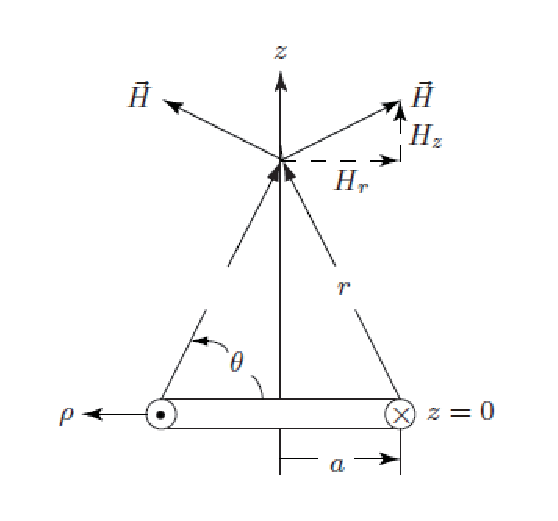
\includegraphics[scale=0.7]{chpt3/figs/fig3.1.eps}
  \caption{半径为a的闭合回路通过电流I}
\end{figure}

式中,$\cos\theta=a/r$,$r^2=a^2+z^2$,于是$H_z(z,\rho)$在z轴上($\rho=0$)成为:
\begin{eqnarray}\label{eqn:bs law z2}
H_z(z,0)&=&\frac{a^2I}{2r^3}=\frac{a^2I}{2(a^2+z^2)^{3/2}} \nonumber \\
H_z(z,0)&=&\frac{H_z(0,0)}{(1+(z/z)^2)^{3/2}} \mbox{(\quad 以中心处磁场$H_z(0,0)$表示)}
\end{eqnarray}
专题1将以实例进行进一步的讨论。

\section{Lorentz力和磁压}
在有磁感应强度$\vec{B}$存在时,以速度$v$运动的电荷$q$会受到力$\vec{F}_L$,此力称为Lorentz力:
$\vec{F}_L=q\vec{v}\times \vec{B}$。对于一个电流密度为$J$的导体,在磁场$\vec{B}$中,所受Lorentz力密度为
\begin{equation}\label{eqn:lorentz force}
  \vec{f}_L=\vec{J}\times \vec{B}
\end{equation}
方程\ref{eqn:lorentz force}是磁体中电磁力和应力的基本表达式。如第一章开始提到的,不管是以超导运行于1.8-80K,还是以有阻态运行于室温,产生相同磁场的磁体所需要处理的应力水平基本是一样的。磁体
的极限磁场为结构部件和载流导体的强度所限。这样看,一个50T的超导磁体——如果可能的话——和一个
50T有电阻磁体都必须承受巨大的Lorentz应力。下文将说明,一个50T磁体的等效磁压约为
1GPa(10000atm)。

考虑一个无限长的薄壁螺线管,半径为$2a$,通以均匀分布的电流(为了简化为面电流密度
$K_\theta [A/m]$计算)。$(0,0)$处的磁感应强度的z分量为
\begin{equation}\label{eqn:inf solenoid}
  B_z=\frac{\mu_0 a^2 K_\theta}{2}\int_{-\infty}^{\infty}\frac{dz}{(a^2+z^2)^{3/2}=\mu_0 K_\theta}\equiv B_0
\end{equation}
由于电流环的分布是从$z=-\inf$到$z=\inf$的,积分包括整个z轴。应用Ampere定律,可知对于无限长
螺管,螺管外($r>a$)的$\vec{B}$为零;螺管内在z和r两个方向都是均匀的$B_0$。也就是说,无限长螺管的室温孔内的磁场时完全均匀的,并且仅在z向。

绕组内部的$B_z$是$B_0$,外部是0,在管壁厚度$\delta$方向线性正比于$r$衰减。所以,平均磁感应强度$\bar{H}_z$是$B_0/2$。因而,r方向施于线圈上的平均Lorentz力密度为
\begin{equation}\label{eqn:inf solenoid fl}
  f_{L_r}\vec{i}_r=\frac{K_\theta}{\delta}B_z \vec{i}_r=\frac{K_\theta B_0}{2\delta}\vec{i}_r
\end{equation}

\begin{figure}[htbp]
  \centering
 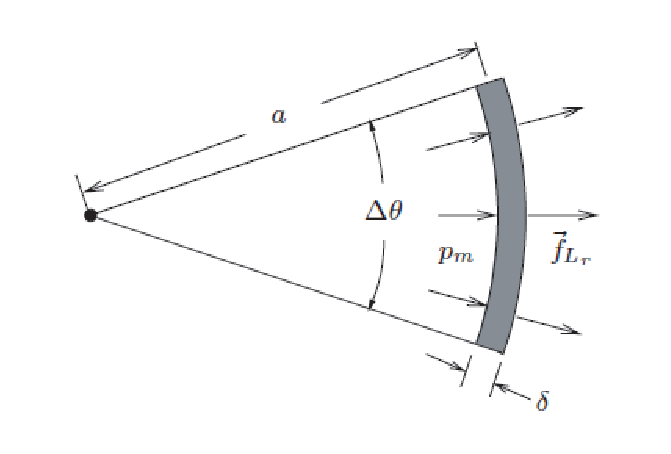
\includegraphics[scale=0.6]{chpt3/figs/fig3.2.eps}
  \caption{平均直径为2a的薄壁螺管(壁厚$\delta$)的微元的轴向视角}
\end{figure}
作用于线圈体积元上的r向的Lorentz力$F_{L_r}\vec{i}_r$等价于作用于线圈表面元上的磁压$p_m\vec{i}_r$。
于是
\begin{equation}\label{eqn:inf solenoid fl2}
  F_{L_r}\vec{i}_i =f_{L_r}[(a\Delta \theta)\delta \Delta z]\vec{i}_r=p_m[(a\Delta \theta)\Delta z]\vec{i}_r
\end{equation}
联立上式,可得
\begin{equation}\label{eqn:mag press}
  p_m=\frac{B_0^2}{2\mu_0}
\end{equation}
也即,磁压等于磁能密度。如果磁感应强度$B_0=1 T$ ,可算得磁压为$3.98\times 10^5 Pa$或者
$~4 atm$。容易算出如果$B_0=50 T$,磁压将达到$~1 GPa$。

\section{螺管线圈的场分析}
本节,我们将推导出对分析高空间场均匀性的MRI和NMR磁体有用的闭式场表达式以及简单线圈(“长”、“薄”)的表达式。
在螺管线圈设计的开始阶段,可以用这些表达式来对场的均匀性“找找感觉”。

图3.3给出的是一个内径、外径和长度分别为$2a_1, 2a_2, 2b$的螺管线圈的剖面图。从磁力线可以看出,线圈产生的磁场在室温孔内
主要是轴向的,除了线圈的对称轴和轴平面上的径向,磁力线都是发散的,室温孔外尤甚。用于螺管线圈磁场分析的两个无量纲常数为:
$\alpha\equiv 2a_2/2a_1=a_2/a_1$和$\beta\equiv 2b/2a_1=b/a_1$。外径和长度都规范化为内径了。
\begin{figure}[htbp]
	\centering
	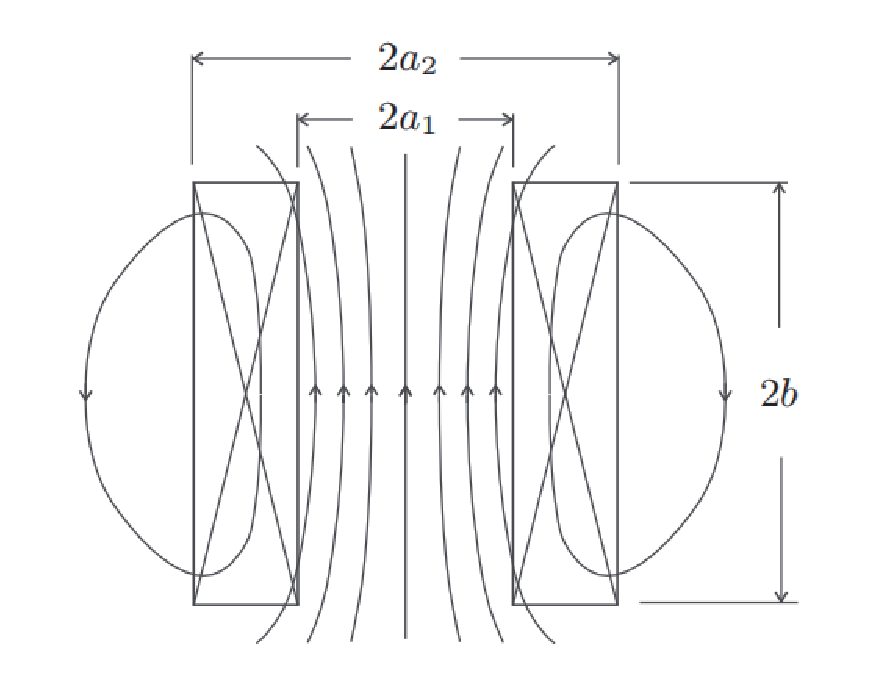
\includegraphics[scale=0.5]{chpt3/figs/fig3.3.eps}
	\caption{螺管线圈的截面视图}
\end{figure}

在球坐标系$(r,\theta,\phi)$下,任何电流体系和/或磁性材料产生的z向磁场$H_z(r,\theta,\phi)$在除源以外空间可以写为:
\begin{equation}\label{eqn:solenoid coil hz}
  H_z (r,\theta,\phi)=\Sigma_{n=0}^\infty \Sigma_{m=0}^n r^n (n+m+1) P_n^m(u)(A_n^m\cos m\phi+B_n^m\sin m\phi)
\end{equation}
式中,$P$是Legendre多项式。

$A_n^m$和$B_n^m$是常数,通常除了$A_0^0$和$B_0^0$都是要被最小化的,因为它们是引起不均匀性的项。$A_n^m$和$B_n^m$
可以通过调节磁体中每一个线圈的参数来最小化。这些参数包括线圈内径、外径、长度、中平面相对于磁中心的位置、总体电流密度等。
简单说,所有与磁场的空间分布有关的参数都仅仅是无量纲参数$\alpha, \beta$的函数。
\begin{figure}[htbp]
	\centering
	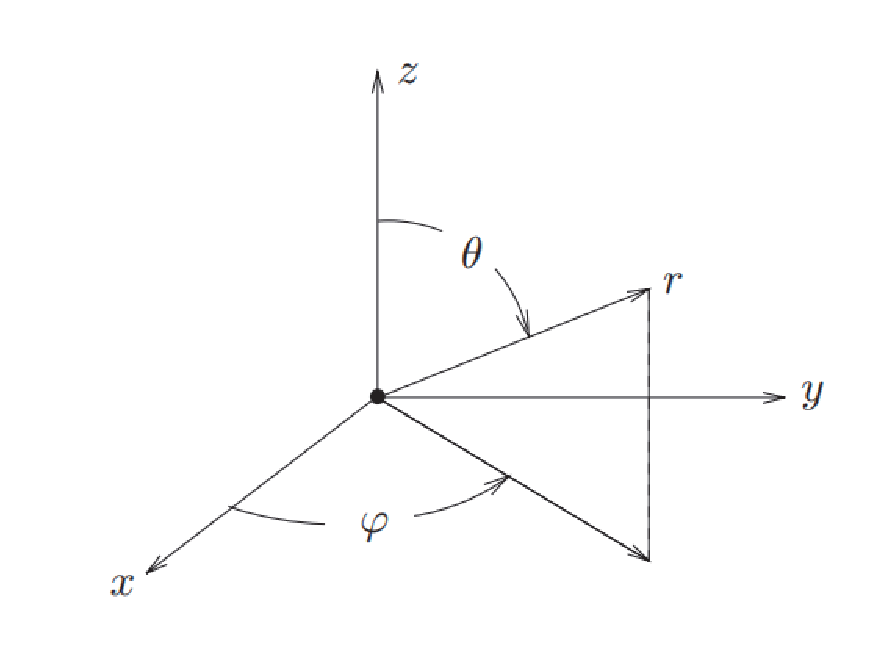
\includegraphics[scale=0.5]{chpt3/figs/fig3.4.eps}
	\caption{圆柱坐标}
\end{figure}

螺管系统中,所有的电流密度与$\phi$无关,即存在轴对称性。此时,仅$m=0$的项保留。沿着z轴($r=z,\theta=0$)和沿着中平面上的
x(或y)轴($x,\theta=90^\circ$),磁场化简:
\begin{eqnarray}\label{eqn:solenoid coil hz1}
H_z(z)&=&\Sigma_{n=0}^\infty z^n(n+1)A_n^0 \nonumber \\
H_z(x)&=&\Sigma_{n=0}^\infty \Sigma_{m=0}^n x^n(n+m+1)P_n^m(0)A_n^m\
\end{eqnarray}
上式第一式不含Legendre函数,因为$P_n^0(1)=P_n(1)=1$。第二式中,注意到当n=偶数且m=奇数时,$ P_n^m(0)=0$。代入n和m的0,2,4三个值,
我们可以写出笛卡尔坐标系下的$H_z(x)$
\begin{eqnarray}\label{eqn:solenoid coil hz2}
H_z(z)&=&A_0^0+3A_2^0z^2+5A_4^0z^4+\cdots \nonumber \\
H_z(x)&=&A_0^0-(3/2A_2^0-15A_2^2)x^2+(15/8 A_4^0-105/2 A_4^2\nonumber\\
&& +945A_4^4)x^4+\cdots
\end{eqnarray}
式中,$A_0^0$是磁体中心$(0,0,0)$的场:$A_0^0\equiv H_)$。理想螺管中,对于$m>0$时,系数为0:$A_0^0=0$。对于$n>0, m=0$时,$A_n^0$
是线圈参数$\alpha, \beta$的函数。引入$h_z(\zeta)\equiv H_z(z)/H_0$,此处$\zeta \equiv z/a_1, h_z(\xi)\equiv H_z(x)/H_0, \xi\equiv x/a_1$,我们
得到
\begin{eqnarray}\label{eqn:solenoid coil hz2}
h_z(\zeta)&=&1+E_2(\alpha,\beta)\xi^2+E_4(\alpha,\beta)\zeta^4+E_6(\alpha,\beta)\zeta^6+\cdots \nonumber \\
h_z(\xi) &=&1-\frac{1}{2}E_2(\alpha,\beta)\xi^2+\frac{3}{8}E_4(\alpha,\beta)\xi^4-\frac{5}{16}E_6(\alpha,\beta)\xi^6+\cdots
\end{eqnarray}
注意到$\xi^2$的系数仅为$\zeta^2$系数异号的一半,$\xi^4$的系数为$\zeta^4$同号的$\frac{3}{8}$。实际上,平面方向的任何系数在数值上都小于z向。
所以,x和y方向的场的不均匀性要比z向小。

中心场$H_0(\equiv A_0^0)$由下式给出:
\begin{eqnarray}\label{eqn:h0}
  H_0&=&\lambda J a_1 F(\alpha,\beta)=\lambda J a_1 \beta \ln [\frac{\alpha+\sqrt{\alpha^2+\beta^2}}{1+\sqrt{1+\beta^2}}]  \nonumber \\
  F(\alpha,\beta)&=&\beta \ln [\frac{\alpha+\sqrt{\alpha^2+\beta^2}}{1+\sqrt{1+\beta^2}}]
\end{eqnarray}
式中,$F(\alpha,\beta)$是均匀电流密度线圈的”磁场因子“。上式的衍生问题在专题3.1进行讨论。$E_n (\alpha,\beta)$在$n=2,4,6,8,10$时的表达式
在下面以$F(\alpha,\beta)$和$E_n(\alpha,\beta)$的乘积的形式给出:
\begin{eqnarray}
 F(\alpha,\beta) E_2(\alpha,\beta)&=& \frac{1}{2\beta}[\frac{1}{(1+\beta^2)^{1.5}} - \frac{\alpha^3}{(\alpha^2+\beta^2)^{1.5}}]
\end{eqnarray}
\begin{eqnarray}
 F(\alpha,\beta) E_4(\alpha,\beta)&=& -\frac{r^3}{24\beta^3}[\frac{2+7\beta^2+20\beta^4}{(1+\beta^2)^{3.5}} - \frac{2\alpha^7+7\alpha^5 \beta^2+20\alpha^3\beta^4}{(\alpha^2+\beta^2)^{3.5}}] \nonumber
\end{eqnarray}
上式还可写为更简洁的形式:
$$F(\alpha,\beta) E_4(\alpha,\beta)=-\frac{r^3}{24\beta^3}\left[\frac{2r^4+7r^2\beta^2+20\beta^4}{(\alpha^2+\beta^2)^{3.5}}\right]|_{r=1}^{r=\alpha}$$

以下分别为6阶、8阶的形式:
$$F(\alpha,\beta) E_6(\alpha,\beta)=-\frac{r^3}{240\beta^5}\left[\frac{8r^8+44 r^6\beta^2+99 r^4\beta^4+28 r^2 \beta^6+280 \beta^8}{(\alpha^2+\beta^2)^{5.5}}\right]_{r=1}^{r=\alpha}$$
$$F(\alpha,\beta) E_8(\alpha,\beta)=-\frac{r^3}{896\beta^7}\left[\frac{16 r^{12}+120 r^{10}\beta^2+390..+715..+1080..-1008..+1344..}{(\alpha^2+\beta^2)^{7.5}}\right]_{r=1}^{r=\alpha}$$


$F(\alpha,\beta) E_{n}(\alpha,\beta)$是一个递归式,第$n$阶项可以写为:
\begin{equation}
  F(\alpha,\beta) E_{n}(\alpha,\beta)=\frac{1}{n} \frac{\partial}{\partial \beta}\left[F(\alpha=1,\beta)E_{n-1}(\alpha=1,\beta)-F(\alpha,\beta)E_{n-1}(\alpha,\beta)\right]
\end{equation}
或者写为
$$ F(\alpha,\beta) E_{n}(\alpha,\beta)=\frac{1}{M_n \beta^{n-1}}\left[\frac{f_n(\alpha=1,\beta)}{(1+\beta^2)^{n-0.5}}-\frac{\alpha^3 f_n(\alpha,\beta)}{(\alpha^2+\beta^2)^{n-0.5}}\right]$$
式中,$M_n$是一个常数。附录给出了$n=2,3,4,...20$时的$M_n$和$f_n(\alpha,\beta)$的值。20之下的偶数$f_n$用来求解磁场问题。

一般来说(但也不全是),z轴向磁场$H_z(z)$的均匀性要比z轴法平面上的均匀性更好。故,我们仅考虑z轴向磁场
$$\frac{\partial^2 h_z(\zeta)}{\partial \zeta^2}=[2 E_2(\alpha,\beta)+(4)(3)E_4(\alpha,\beta)\zeta^2+...]=\Sigma_{n=1}^{\infty} (2n)(2n-1)E_{2n}(\alpha,\beta)\zeta^{2(n-1)}$$

一般有,
\begin{equation}
 \frac{\partial^{2k} h_z(\zeta)}{\partial \zeta^{2k}}=\Sigma_{n=k}^{\infty} (2n)(2n-1)(\cdots)(2n-2k+1)E_{2n}(\alpha,\beta)\zeta^{2(n-k)}
\end{equation}

在原点处,$\zeta=0$。上两式由于仅第一项非零,可以化为更简单的形式
$$\frac{\partial^2 h_z(\zeta)}{\partial \zeta^2}|_{0}=2 E_{2}(\alpha,\beta)$$
\begin{equation}
 \frac{\partial^{2k} h_z(\zeta)}{\partial \zeta^{2k}}|_{0}=(2k)! E_{2k}(\alpha,\beta)
 \end{equation}

\textbf{嵌套线圈磁体}

由$\ell$个线圈同心同轴嵌套的磁体,3.12a式仅给出$\zeta^2$项,对每一组$\lambda J, a_1, \alpha, \beta$,有通用表达式
\begin{equation}
  h_z(\zeta)=1+\frac{\Sigma_{j=1}^{\ell} (\lambda J)_l a_{1_j}F(\alpha_j,\beta_j)E_2(\alpha_j,\beta_j)}{\Sigma_{j=1}^{\ell}(\lambda J)_j a_{1_j} F(\alpha_j,\beta_j)}\zeta^2+\cdots
\end{equation}

\subsection{简单线圈}
本节我们推导“简单”线圈的$E_n(\alpha,\beta)$和$h_z(\zeta)$在10阶以下的表达式。各$h_z(\zeta)$的表达式可以给设计者在不依赖于磁场分析专家时,对考虑线圈尺寸(即$\alpha, \beta$)的线圈的场
的均匀性有一个“感觉”。
\subsubsection{“短”线圈}
短线圈($\beta\rightarrow 0 $),如饼式线圈,其$F(\alpha,\beta)$简化为
\begin{equation}
  F(\alpha,\beta\rightarrow 0)=\beta \ln\alpha
\end{equation}

通过枯燥的推导,从3.14可以得出$E_2,\cdots,E_{10}$。在$\beta\rightarrow 0$极限下,$f_n(\alpha,\beta)$分母$(1+\beta^2)^{n-0.5}$可以展开
为$\beta^{2k}$的级数,取前n项。整数k取遍1至n/2.
\begin{equation}
 \frac{1}{(1+\beta^2)^{n-0.5}}=1+...+(-1)^k (n-0.5)\cdots(n+k-1.5)\frac{\beta^{2k}}{k!}
\end{equation}

在$\beta\rightarrow 0$极限下,上式右侧高于$\beta^n$的项为高阶小,可以忽略。同时,所有小于$\beta^n$的项都被约掉,仅剩下$\beta^n$项。
\begin{eqnarray}
% \nonumber % Remove numbering (before each equation)
  E_2(\alpha,0) &=& -\frac{3}{2^2}\frac{(\alpha^2-1)}{\alpha^2 \ln \alpha}=-\frac{3(\alpha^2-1)}{4\alpha^2 \ln \alpha} \\ \nonumber
  E_4(\alpha,0) &=& \frac{15(\alpha^4-1)}{32\alpha^4 \ln \alpha} \\ \nonumber
  E_6(\alpha,0) &=& -\frac{35(\alpha^6-1)}{96\alpha^6\ln \alpha} \\ \nonumber
  E_8(\alpha,0) &=& \frac{315(\alpha^8-1)}{1024\alpha^8 \ln \alpha} \\ \nonumber
    E_{10}(\alpha,0) &=& -\frac{693(\alpha^{10}-1)}{2560\alpha^{10} \ln \alpha}
\end{eqnarray}

3.12a于是成为
\begin{equation}
  h_z(\zeta)=1-\frac{3(\alpha^2-1)}{4\alpha^2 \ln \alpha}+\frac{15(\alpha^4-1)}{32\alpha^4 \ln \alpha} -\frac{35(\alpha^6-1)}{96\alpha^6\ln \alpha}+\cdots
\end{equation}

\subsubsection{“薄壁”线圈}
对于薄壁线圈($\alpha=1$),$F(\alpha,\beta)$成为
\begin{equation}
  \lim_{\alpha\rightarrow 1} F(\alpha,\beta)=\beta\frac{\epsilon}{\sqrt{1+\beta^2}}=\frac{\beta(\alpha-1)}{\sqrt{1+\beta^2}}
\end{equation}

联立3.13和上式,得到:
\begin{eqnarray}
% \nonumber % Remove numbering (before each equation)
  E_2(1,\beta) &=& -\frac{3}{2(1+\beta^2)^2} \\ \nonumber
  E_4(1,\beta) &=& \frac{5(3-4\beta^2)}{2^3(1+\beta^2)^4} \\ \nonumber
    E_6(1,\beta) &=& -\frac{7(5-20\beta^2+8\beta^4)}{2^4 (1+\beta^2)^6} \\ \nonumber
      E_8(1,\beta) &=& \frac{9(35-280\beta^2+336\beta^4-64\beta^6)}{2^7(1+\beta^2)^8} \\ \nonumber
        E_{10}(1,\beta) &=& -\frac{11(63-840\beta^2+2016\beta^4-1152\beta^6+128\beta^8)}{2^8(1+\beta^2)^{10}}
\end{eqnarray}

于是,对于薄壁线圈,我们有:
\begin{equation}
  h_z(\zeta)=1-\frac{3}{2(1+\beta^2)^2} +\frac{5(3-4\beta^2)}{2^3(1+\beta^2)^4}+\cdots
\end{equation}

\subsubsection{“薄壁且长”线圈}
对于“薄壁且长”线圈($\alpha=1,\beta\rightarrow \infty$),3.25式简化为
\begin{equation}
  h_z(\zeta)=1-\frac{1.5}{\beta^4}\zeta^2-\frac{2.5}{\beta^6}\zeta^4-\frac{3.5}{\beta^8}\zeta^6-\cdots-\frac{n+1}{2\beta^{n+2}}\zeta^{n}
\end{equation}

从上式可以得出,在$\beta\rightarrow \infty$极限下,$E_n(1,\beta)=-(n+1)/2\beta^{(n+2)}$。正如我们所预期的,随线圈长度增加,均匀度提高。

\subsubsection{“环”线圈}
对环形线圈($\alpha=1,\beta=0$),$E_n(\alpha,\beta)$可由3.21在极限$\alpha=1$以及3.25在极限$\beta=0$下推出。在3.21中,
\begin{equation}
  \lim_{\alpha\rightarrow 1}\frac{\alpha^n-1}{\alpha^n \ln\alpha}=n
\end{equation}

联立3.21和上式,或者简单的在3.24式中令$\beta=0$,可以得到同样的结果:
\begin{eqnarray}
% \nonumber % Remove numbering (before each equation)
  E_2(1,0) &=& -\frac{3}{2}=-1.5 \\ \nonumber
  E_4(1,0) &=& \frac{3\cdot 5}{2^3}=1.875 \\ \nonumber
    E_6(1,0) &=& -\frac{3\cdot 5 \cdot 7}{2\cdot 4\cdot 6}\simeq-2.188 \\ \nonumber
      E_8(1,0) &=&\frac{3\cdot 5 \cdot 7\cdot 9}{2\cdot 4\cdot 6\cdot 8}\simeq 2.461 \\ \nonumber
        E_{10}(1,0) &=-&\frac{3\cdot 5 \cdot 7\cdot 9\cdot 11}{2\cdot 4\cdot 6\cdot 8\cdot 10}\simeq -2.707
\end{eqnarray}

于是
\begin{equation}
  h_z(\zeta)=1-1.5\zeta^2+1.875\zeta^4-2.188\zeta^6+\cdots
\end{equation}

\subsection{失谐—嵌套双线圈磁体}
方程3.12表明,$h_z(\zeta)$和$h_z(\xi)$(其中,$h_z(\zeta)\equiv H_z/H_0,\zeta\equiv z/a_1,\xi\equiv x/a_1$)都仅与$\zeta$或$\xi$的偶次幂有关。也即,两个方程都表达了“理想”螺线管或者此种“理想”嵌套螺管的轴向场的空间变化。在这里,“理想”指的是空间对称性、均匀性以及电流密度的不变性。

哪怕对一个单螺管,现实也是很不同的:线圈形状的瑕疵;导体尺寸和形状;导体的放置导致不仅与偶次幂有关。如果一个磁体是由嵌套线圈组成的,可能的瑕疵就更多了,会出现很多“不希望”的项。下面,我们将展示嵌套双线圈磁体失谐的起源。

考虑一个双螺管线圈嵌套磁体,参数为$[2a_1]_1,\alpha_1,\beta_1,[\lambda J]_1$的螺管线圈1嵌入参数为$[2a_1]_2,\alpha_2,\beta_2,[\lambda J]_2$的螺管线圈2内。如果两个线圈在轴向和径向都对齐的话,有:
\begin{equation}
H_z(z)=[H_z(z)]_1+[H_z(z)]_2
\end{equation}
式中,$[H_z(z)]_1$和$[H_z(z)]_2$由下式给出:
\begin{eqnarray}
  [H_z(z)]_1 &=& [A_0^0]_1 +3[A_2^0]_1 z^2+5[A_4^0]_1 z^4+... \\ \nonumber
  [H_z(z)]_2 &=& [A_0^0]_2 +3[A_2^0]_2 z^2+5[A_4^0]_2 z^4+...
\end{eqnarray}

注意到,中心的总轴向场有:$H_z(0)=[A_0^0]_1+[A_0^0]_2\equiv H_0$

\subsubsection{线圈轴向失配}
如果线圈1和线圈2在径向是对齐的,即同轴。但是两个线圈的中心面未对齐,分别在$z=0$和$z=\delta_z$。这样,3.31中的$H_z(z)$成为:
\begin{equation}
  H_z(z)=H_0+3\{ [A_2^0]_1 z^2+[A_2^0]_2(Z-\delta_z)^2\}+5\{[A_4^0]_1 z^4+[A_4^0]_2(z-\delta)^4\}+\cdots
\end{equation}

展开上式中的乘方项,有:
$$H_z(z)=\{H_0+3[A_2^0]_2 \delta_z^2+5[A_4^0]_2\delta_z^4+\cdots\}-\{6[A_2^0]_2\delta_z+20[A_4^0]_2\delta_z^3+\cdots\}+\cdots$$

从上式可以看出,线圈1和线圈2的轴向失配$\delta_z$不仅影响了各含$z$项的系数,更重要的,还增加了z的奇次幂项,这导致$H_z(z)$在轴向不在对称。

在实际由许多线圈嵌套组成的NMR磁体中,轴向失配是不可避免的。例如,含$z$项要么扩大NMR谱线,要么引起谱线中各峰值的“下沉”。$z^3$项同样扩大了谱线,不过主要是在偏离中心频率的地方。

\subsubsection{轴向补偿线圈}
那些“不希望”的项可以经由超导磁体内部增加的补偿/校正线圈最小化。甚至,补偿线圈还可以布置在探测器和低温容器室温孔之间的径向间隙中。

最小化z的偶次幂项的补偿线圈本质上是“Helmholtz”线圈,其基本问题我们将在问题3.3中研究。最小化z的奇次幂的补偿线圈同样是Helmholtz类型的,但是它的一个线圈是反极性的,以产生轴向反对称场。

\subsubsection{线圈径向失配}
为了研究径向失配的嵌套双线圈磁体的磁场的空间变化,我们首先在笛卡尔坐标系中写出单个螺线管的$H_z(x,y,z)$。从方程3.11和Legendre函数表的$n=0,n=2,n=4$条,我们有:
\begin{equation}
  H_z(x,y,z)=A_0^0+3A_2^0[z^2-\frac{1}{2}(x^2+y^2)]+5A_4^0\{z^4-3(x^2+y^2)[z^2-\frac{1}{8}(x^2+y^2)]\}
\end{equation}

当线圈2相对于线圈1在径向失配,在x方向失配$\delta_x$,在y方向失配$\delta_y$。我们将上式中的x和y分别用$x-\delta_x$和$y-\delta_y$替换,有:
$$
H_z(x,y,z)=H_0+3()+5()+[A_4^0]_2()
$$

上面的展开式包含很多项,包括$x,x^2,x^3,x^4,y,y^2,y^3,y^4,xy,xy^2,z^2,z^2x...$等等。

一个x向补偿线圈通常由一对薄的(一层或几层导体厚)成型为“鞍状”以适应磁体的外圆柱表面并且其轴向沿$\phi=0(x)$方向布置的长方形线圈构成。它产生一个随x增大的z向磁场,在z轴($x=0$)处为0。类似的,y向补偿线圈和xy补偿线圈分别是沿着$\phi=90^\circ$和$\phi=45^\circ$成对布置的。每个线圈产生一个z向磁场,随z轴增大。

\subsubsection{线圈轴向、径向均失配}
当嵌套线圈在轴向和径向均失配的时候——实际NMR中不可避免的结果——xz,yz,xyz及其他更多的失调会产生。

\section{轴向力}
本节给出轴向对齐环形线圈、薄壁螺管线圈等的轴向力$F_z$的解析表达式。这些表达式都是从Garrett [3.5]给出的公式推导出来的。极限情况下(比如相距很远的线圈)的近似表达式有助于快速的数值检查;另一些公式或许可以用于为写自己的计算代码做基础。所有的案例中,电流都是同向流动的,任一个电流的反向都将导致力的反向。

\subsection{两个“环”线圈间的轴向力}
图3.5给出了距离为$\rho$、轴向分立的两个“环”线圈($\alpha=1,\beta=0$)。线圈A和线圈B的直径分别为$2a_A$和$2a_B$,总的安匝数分别为$N_A I_A$和$N_B I_B$。每个线圈产生的轴向场都指向同一方向。线圈B施于线圈A的轴向力$F_{zA}(\rho)$为:
\begin{figure}[htbp]
	\centering
	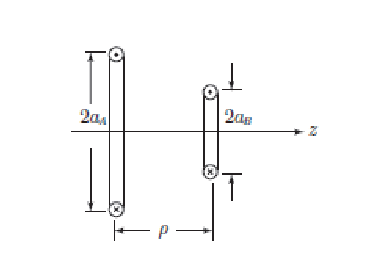
\includegraphics[scale=1]{chpt3/figs/fig3.5.eps}
	\caption{“环”线圈A和B同轴对齐,距离上相距$\rho$}
\end{figure}

\begin{equation}
  F_{ZA}(\rho)=\frac{\mu_0}{2}(N_A I_A)(N_B I_B)\frac{\rho\sqrt{(a_A+a_B)^2+\rho^2}}{(a_A-a_B)^2+\rho^2}\times\{k^2 K(k)+(k^2-2)[K(k)-E(k)]\}
\end{equation}

$F_{zA}(\rho)$是+z向或者说是指向线圈B的;也即,$F_{zA}(\rho)$是吸引力。如果两个电流的方向相反,符号变为-,力变成斥力。上式中,$K(k)$和$E(k)$分别是第一类和第二类完全椭圆积分,定义为:
\begin{eqnarray}
% \nonumber % Remove numbering (before each equation)
  K(k) &=& \int_{0}^{\pi/2} \frac{d\theta}{\sqrt{1-k^2\sin^2\theta}} \\ \nonumber
  E(k)&=& \int_{0}^{\pi/2}\sqrt{1-k^2 \sin^2\theta}d\theta
\end{eqnarray}
本系统椭圆积分的模量k由下式决定:
\begin{equation}
  k^2=\frac{4a_A a_B}{(a_A+a_B)^2+\rho^2}
\end{equation}



%%%%%%%%表格3.1
\begin{table}
\centering
\caption{第一类和第二类椭圆积分参数值}
\label{my-label}
\begin{tabular}{|c|c|c|c|c|c|c|c|}
\hline
$k^2$    & $k$  & $K(k)$ &$E(k)$  &$k^2$  & $k$ &$K(k)$  &$E(k)$  \\ \hline
0   & 0 &$pi/2$  & $pi/2$ &0.7&0.8367  &2.0754  & 1.2417 \\ \hline
0.1 & 0.3162  & 1.6124 &1.5308  &0.8& 0.8944 & 2.2572 & 1.1785 \\ \hline
0.2 & 0.4472  & 1.6596 &1.4890  &0.9&0.9487  & 2.5781 & 1.1048 \\ \hline
0.3 & 0.5477  & 1.7139 & 1.4454 &0.95&0.9747  &2.9083  & 1.0605 \\ \hline
0.4 & 0.6325  & 1.7775 &1.3994  &0.98& 0.9899 & 3.3541 & 1.0286 \\ \hline
0.5 & 0.7071  & 1.8541 &1.3506  & 0.99& 0.9950 &3.6956  & 1.0160 \\ \hline
0.6 & 0.7746  & 1.9496 &1.2984  &1  &1  &$\infty$  &  1\\ \hline
\end{tabular}
\end{table}

表3.1给出了部分$k$和$k^2$值下的$K(k)$和$E(k)$。注意到,$K(0)=E(0)=\pi/2$;还注意到,$K(1)=\infty$以及$E(1)=1$,也即$K(k)$是随k增加而增加的,$E(k)$随k增加而减小。
$K(k)$和$E(k)$可以展开为$k^2$的级数:
\begin{eqnarray}
% \nonumber % Remove numbering (before each equation)
  K(k) &=& \frac{\pi}{2}[1+(\frac{1}{2})^2 k^2+(\frac{1\cdot 3}{2\cdot 4})^2 k^4+(\frac{1\cdot 3\cdot 5}{2\cdot 4\cdot 6})^2 k^6+\cdots] \\ \nonumber
  E(k) &=& \frac{\pi}{2}[1-(\frac{1}{2})^2 k^2-(\frac{1\cdot 3}{2\cdot 4})^2 \frac{k^4}{3}-(\frac{1\cdot 3\cdot 5}{2\cdot 4\cdot 6})^2 \frac{k^6}{5}-\cdots]
  \end{eqnarray}

在$k^2\ll 1$时,两个积分和他们的差可以近似为
\begin{eqnarray}
% \nonumber % Remove numbering (before each equation)
  K(k) &\simeq&  \frac{\pi}{2}(1+\frac{1}{4}k^2+\frac{9}{64}k^4+\frac{25}{256}k^6+\frac{1225}{16384}k^8)\\ \nonumber
  E(k) &\simeq&  \frac{\pi}{2}(1-\frac{1}{4}k^2-\frac{3}{64}k^4-\frac{5}{256}k^6-\frac{175}{16384}k^8)\\ \nonumber
  K(k)-E(k) &\simeq& \frac{\pi}{4}(k^2+\frac{3}{8}k^4+\frac{15}{64}k^6+\frac{175}{1024}k^8) 
\end{eqnarray}

\subsubsection{特例1:两个远离的“环”线圈}
当两个线圈相距足够远,也即$\rho^2 \gg (a_A+a_B)^2$时,有$k^2\ll 1$。此时,可以用方程3.38化简3.34。方程3.34首先被简化为:
$$
  F_{zA}(\rho)\simeq \frac{\mu_0}{2}(N_A I_A)(N_B I_B)\{ k^2K(k)+(k^2-2)[K(k)-E(k)]\}
\eqno{(3.39a)}$$

应用3.38第一式和第三式,仅考虑$k^4$及以下项。尽管$k^2\ll 1$,我们展开$K(k)-E(k)$时必须将$k^4$项包括进来,因为它的系数还有一个$-2$:
$$
F_{zA}(\rho)\simeq \frac{\mu_0}{2}(N_A I_A)(N_B I_B)(\frac{3\pi}{16}k^4) \eqno{(3.39b)}
$$

在第二步近似时,$k^6$项被略去了。最后,我们得到了极限$\rho^2 \gg (a_A+a_B)^2$时的一个简单表达式:
$$F_{zA}(\rho)= \frac{3\mu_0}{2\pi}(\frac{\pi a_A^2 N_A I_A}{\rho^2})(\frac{\pi a_B^2 N_B I_B}{\rho^2}) \eqno{(3.39c)}$$

\subsubsection{特例2:两个紧邻的相同直径的“环”线圈}
如果两个环线圈的直径相同并相互紧邻放置,即$a_A=a_B=a$以及$\rho\ll 2a$。此时,$k^2\mapsto 1,K(k)\mapsto\infty,E(k)\mapsto 1$。方程3.34可以简化为:
$$F_{zA}(\rho)\simeq \mu_0(N_A I_A)(N_B I_B)(\frac{a}{\rho})\eqno{(3.39d)}$$

我们可以将上式表示为“环”A直径($2\pi a$),“环”A安匝($N_A I_A$)和轴向相距$\rho$处的“环”B在“环”A上的场的径向分量($B_r$,由于$rho\ll a$,可简史表示为$\mu_0 N_B I_B/(2\pi\rho)$)的乘积。于是:
$$F_{zA}(\rho)\simeq (2\pi a)\times(N_A I_A)\times(\frac{\mu_0 N_B I_B}{2\pi\rho})=\mu_0(N_A I_A)(N_B I_B)(\frac{a}{\rho})$$

\subsection{“薄壁”螺管内的轴向力}
考虑一个直径为$2a$,长度为$2b$,中平面位于$z=0$,通过均匀表面电流$NI/2b$的薄壁($\alpha=1$)螺管线圈。对于这个螺管线圈,距离中平面$z\ge 0$处的轴向力可以表示为:
\begin{equation}
F_z(z)=-\frac{\mu_0}{2}(\frac{NI}{2b})^2\{(b-z)\sqrt{4a^2+(b-z)^2}[K(k_{b_-})-E(k_{b_-})]+(b+z)\sqrt{4a^2+(b+z)^2}[K(k_{b_+})-E(k_{b_+})]-2b\sqrt{4a^2+4b^2}[K(k_{2b})-E(k_{2b})]\}
\end{equation}
椭圆积分模量分别为:
$$k_{b_-}^2=\frac{4a^2}{4a^2+(b-z)^2} ; k_{b_+}^2=\frac{4a^2}{4a^2+(b+z)^2} ;k_{2b}^2=\frac{4a^2}{4a^2+4 b^2}$$

\subsubsection{特例3:端部力}
在$z=b$处,因为有$k_{b_+}=k_{2b}$,所以有$F_z(b)=0$。也即,正如我们所预料到的,一个孤立螺线管端部的轴向力是零。

\subsubsection{特例4:中平面的力}
将$z=0$代入3.40式,我们可以得到中平面($z=0$)处的轴向力$F_z(0)$:
\begin{equation}
  F_z(0)=-\frac{\mu_0}{2}(\frac{NI}{2b})^2\{2b\sqrt{4a^2+b^2}[K(k_{b})-E(k_{b})]-2b\sqrt{4a^2+4b^2}[K(k_{2b})-E(k_{2b})]\}
\end{equation}
式中,$k_{2b}$由下式给出:
$$k_{b}^2=\frac{4a^2}{4a^2+b^2}$$

孤立螺线管在$z$向的轴向压缩力从$0$到$z=b$是逐渐变大,至中平面处取得最大值。

\subsubsection{特例5:长薄壁螺管的中平面的力}
对于一个“长”($\beta\gg 1$或者$k^2\ll 1$)的薄壁螺线管,利用方程3.38,可以将方程3.41a简化为:
$$F_z(0)\simeq-\frac{\mu_0}{2}(\frac{NI}{2b})\pi a^2$$
上式表明,$F_z(0)$在给定表面电流密度值$NI/2b$后,与线圈长度无关。因为长螺管的轴向中心场(问题3.1)有$NI/2b=H_z(0,0)$,我们可以得到:
$$F_z(0)\simeq -\frac{1}{2}\mu_0 H_z^2(0,0)\times\pi a^2$$

这样,$F_z(0)$就等于磁压乘上线圈室温孔的面积。实际上,下面我们将看到,每一个轴向力的表达式都有一个磁压项($\mu_0(NI/2b)^2$)或其等价形式。

\subsection{薄壁螺管和环形线圈间的轴向力}
图3.6给出了一个薄壁螺线管($2a_s,2b_s,N_s I_s/2b_s$)与一个环线圈($2a_R,N_R I_R$)同轴放置的情况。螺管右侧距离环线圈距离$\rho$。各线圈产生的轴向场指向同一方向。螺线管受到的轴向力可以表示为:
\begin{equation}
F_{zS}(\rho)=-\frac{\mu_0}{2}(N_R I_R)(\frac{N_S I_S}{2b_s})\times\\
\left(\sqrt{(a_R+a_S)^2+(\rho+2b_s)^2}\{2[K(k_s)-E(k_s)]-k_s^2K(k_s)\}\\
-\sqrt{(a_R+a_s)^2+\rho^2}\{2[K(k_R)-E(k_R)-k_R^2K(k_R)]\}\right)
\end{equation}
式中,模量为:
$$k_{S}^2=\frac{4a_S a_R}{(a_S+a_R)^2+(2b_S+\rho)^2} ; k_{R}^2=\frac{4a_S a_R}{(a_S+a_R)^2+\rho^2} $$

在方程3.42的等号右侧项中,第二项大于第三项,所以$F_{zS}(\rho)$是正值,也即轴向作用力是吸引力。
\begin{figure}[htbp]
	\centering
	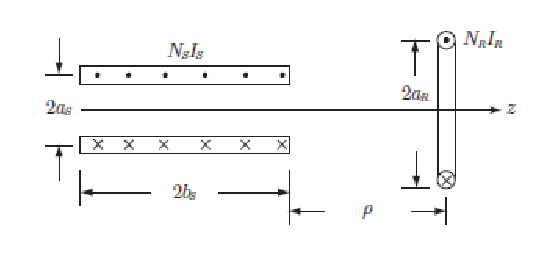
\includegraphics[scale=0.9]{chpt3/figs/fig3.6.eps}
	\caption{薄壁螺管和环形线圈同轴对齐,相距$\rho$}
\end{figure}

\subsubsection{特例6:相距很远的薄壁螺管和环形线圈}
当两个线圈相距很远,也即$k_s^2\ll 1$和$k_R^2\ll 1$时,可以得到:
\begin{equation}
F_{zS}(\rho)=\frac{\mu_0}{2\pi}(\pi a_R^2N_R I_R)(\frac{\pi a_S^2 N_S I_S}{2 b_s})[\frac{1}{\rho^3}-\frac{1}{(\rho+2b_S)^3}]
\end{equation}
按照上述处理方式,我们可以看到力是向着+z方向的,正比于两个线圈磁矩的乘积。

\subsubsection{特例7:相距极远的薄壁螺管和环形线圈}
当两个线圈的相距足够远,以至于$\rho \gg 2b_s$时,方程3.43a中的大括号中的第二项可以展开后略去高次项,有:
\begin{equation}
F_{zS}(\rho)=\frac{\mu_0}{2\pi}(\pi a_R^2 N_R I_R)(\frac{\pi a_S^2 N_S I_S}{2 b_s})\frac{6b_s}{\rho^4}
\end{equation}

正如我们所料,3.43b和3.39c是等价的。
\subsection{两个薄壁螺管间的轴向力}
本节,我们推导两个薄壁螺管之间的轴向力方程。方程是基于Garrett [3.5]的方程推导出来的。
这个方程将成为一般的非薄壁螺线圈的轴向力的基础(3.5.5节)。
考虑两个同轴的薄壁线圈,A($2a_A; 2b_A; N_A I_A/2b_A$)和B ($2a_B; 2b_B;
N_B I_B/2b_B$)。如图3.7所示,螺管A的右端距离螺管B的左端距离为$\rho$。各螺管产生的轴向场是指向同一个方向的。
\subsubsection{螺管B施于螺管A的轴向力}
螺管B施加给螺管A的轴向力可以写为:
\begin{equation}
\begin{split}
F_{zAB}(\rho)=&\frac{\mu_0}{2}(\frac{N_A I_A}{2b_A})(\frac{N_B I_B}{2b_B})\times \\
&(\frac{2b_A+\rho}{\sqrt{a_T^2+(2B_a+\rho)^2}} \{[a_T^2+(2b_A+\rho)^2][K(k_{A})-E(k_{A})]-\Upsilon(c^2,k_A)\}\\
&+\frac{2b_B+\rho}{\sqrt{a_T^2+(2B_B+\rho)^2}} \{[a_T^2+(2b_B+\rho)^2][K(k_{B})-E(k_{B})]-\Upsilon(c^2,k_B) \}\\
&-\frac{2b_T+\rho}{\sqrt{a_T^2+(2B_T+\rho)^2}} \{[a_T^2+(2b_T+\rho)^2][K(k_{T})-E(k_{T})]-\Upsilon(c^2,k_T) \}\\
&-\frac{\rho}{\sqrt{a_T^2+\rho^2}}\{(a_T^2+\rho^2)[K(k_\rho)-E(k_\rho)]-\Upsilon(c^2,k_\rho)\})
\end{split}
\end{equation}
式中,$a_T=a_A+a_B$,$b_T=b_A+b_B$,模量分别为:
$$k_{A}^2=\frac{4a_A a_B}{a_T^2+(2b_A+\rho)^2} ; k_{B}^2=\frac{4a_A a_B}{a_T^2+(2b_B+\rho)^2} $$
$$k_{T}^2=\frac{4a_A a_B}{a_T^2+(2b_T+\rho)^2} ; k_{\rho}^2=\frac{4a_A a_B}{a_T^2+\rho^2} $$

\begin{figure}[htbp]
  \centering
 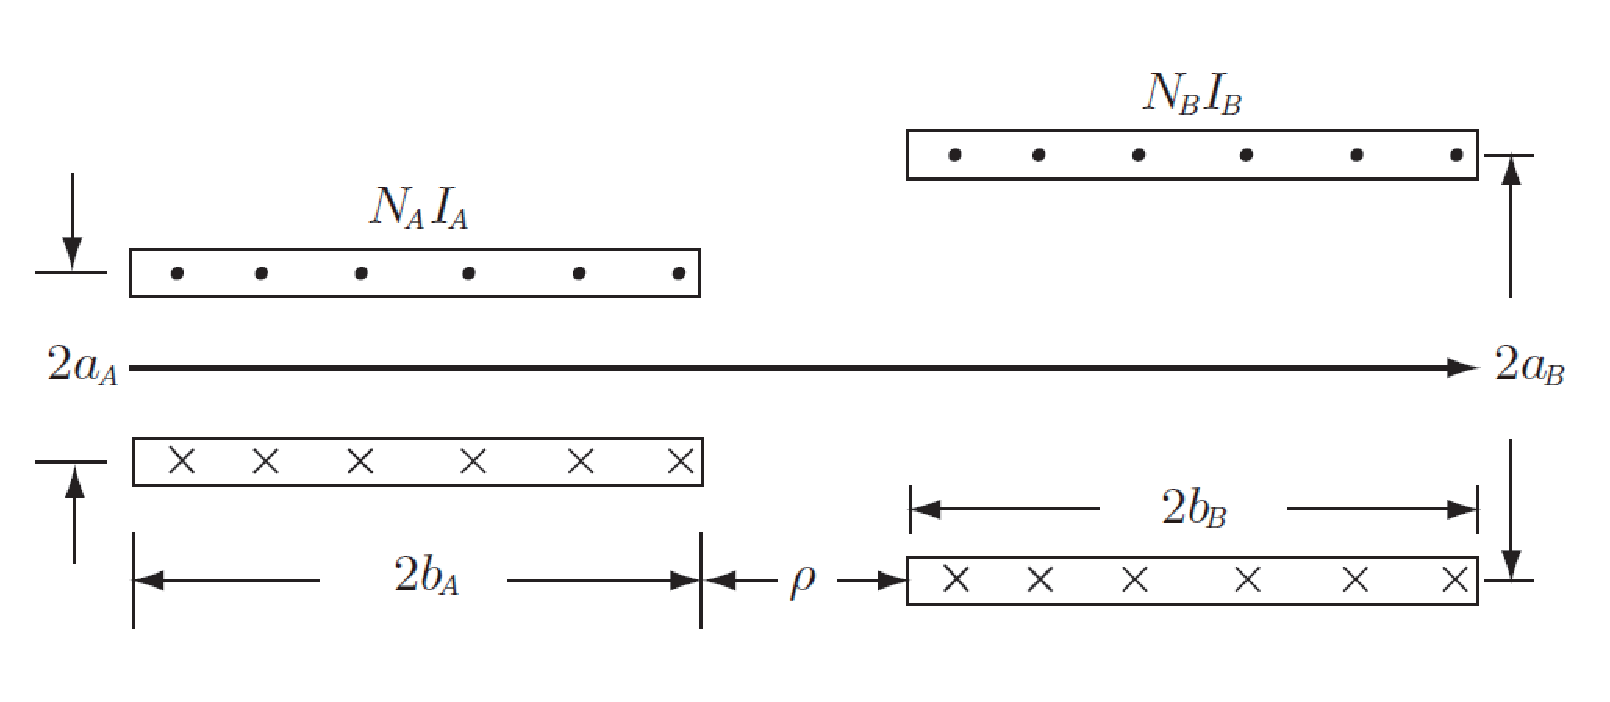
\includegraphics[scale=0.4]{chpt3/figs/fig3.7.eps}
  \caption{薄壁螺管A和B,相距$\rho$}
\end{figure}

上式中,$\Upsilon(c^2,k)$定义为
\begin{equation}
  \Upsilon(c^2,k)\equiv(a_A-a_B)^2[\prod(c^2,k)-K(k)]
\end{equation}
其中,$\prod(c^2,k)$是第三类完全椭圆积分,定义为
\begin{equation}
\prod(c^2,k)=\int_{0}^{\pi/2}\frac{d\theta}{(1-c^2\sin^2\theta)\sqrt{1-k^2\sin^2\theta}}
\end{equation}
从上式明显可以看出,该积分有两个模量:$c^2\le 1$和$k\le 1$。模量$c^2$由下式给出
\begin{equation}
c^2=\frac{4a_A a_B}{a_T^2}=\frac{4a_A a_B}{(a_A+a_B)^2}
\end{equation}
$\prod(0,k)=K(k)$,$\prod(1,k)=\infty$。$\prod(c^2,k)$可用$c^2$和$k^2$的级数表示:
\begin{equation}
\prod(c^2,k)=\frac{\pi}{2}\Sigma_{m=0}^{\infty} \Sigma_{j=0}^{m} \frac{(2m)!(2j)!k^{2j}c^{2(m-j)}}{4^m 4^j (m!)^2(j!)^2}
\end{equation}
低阶项为:
\begin{eqnarray}
% \nonumber % Remove numbering (before each equation)
  \prod(c^2,k) &=& \frac{\pi}{2}(...) \\ \nonumber
  \prod(c^2,0) &=& \frac{\pi}{2}(....)
\end{eqnarray}

注意到,当$c^2=0$时,3.49a退化为3.38a,因为$\prod(0,k)=K(k)$。不过,对于大部分问题,$c^2$通常是接近于1的,这种条件下,由于快速收敛要求$c^2\ll 1$,3.49的任一种展开都不好使。后面,在讨论互感的时候,我们将使用3.49b。表3.2给出了一些$c^2$和$k^2$下的$\prod(c^2,k)$。可以使用Mathcad等软件计算$K(k),E(k),\prod(c^2,k)$。

\subsubsection{特例8:施于A的中平面合力}
我们首先考虑两个螺管A和螺管B具有相同的长度($2b$)、相同的表面电流密度($NI/2b$),但具有不同的直径的情况。对3.44做代换$2b_A = 2b_B = 2b, N_A I_A/2b_A = N_B I_B/2b_B = N I/2b,\rho=0$(线圈相邻端之间无间隙),我们得到线圈A的中平面上的总受力的表达式。这个表达式对于我们探讨非薄壁线圈很有用。
\begin{equation}
\begin{split}
F_{zA}(0)=&\frac{\mu_0}{2}(\frac{NI}{2b})^2\times(  \\
&\frac{4b}{\sqrt{a_T^2+4b^2}} \{[a_T^2+4b^2][K(k_{2b})-E(k_{2b})]-\Upsilon(c^2,k_{2b}) \}\\
&-\frac{4b}{\sqrt{a_T^2+16b^2}} \{[a_T^2+16b^2][K(k_{4b})-E(k_{4b})]-\Upsilon(c^2,k_{4b}) \} )
\end{split}
\end{equation}
式中,$a_T=a_A+a_B$,模量表示为:
$$k_{2b}^2=\frac{4a_A a_B}{a_T^2+4b^2} ; k_{4b}^2=\frac{4a_A a_B}{a_T^2+16b^2} $$

尽管$c^2<1$总是成立的,但$c^2\simeq 1$。对于我们感兴趣的大部分问题,方程3.50不能近似为长螺管线圈($\beta\gg 1$)。

如果我们令线圈A和线圈B直径和表面电流密度一致,但长度减半。当$\rho=0$时这两个螺管线圈就变成了一个长度为$2b$的线圈。接下来,对3.44进行如下替换$2a_A=2a_B=
2a, N_A I_A/2b_A = N_B I_B/2b_B = NI/2b,2b_A = 2b_B = b$,代换后的方程变成3.50.

\subsection{“厚壁”螺管——中平面轴向力}
当一个螺管不能视为薄壁时,可以将之视为在径向上很多薄壁线圈的集合。这里,我们考虑对$\alpha>1$螺管线圈的最简单的处理方法:螺管被分为两个薄壁子螺管A(内)和B(外),两个线圈的长度均为$2b$,直径分别为$2a_A,2a_B$,且有$2a_B >2a_A$。单位长度电流为$1/2(NI/2b)$。一半子线圈A上的总的轴向力由两部分组成:一半来自与它自己的另一半,$F_{zAA}(0)$,可由3.41a给出;一半来自螺管线圈B,$F_{zAB}(0)$。图3.8给出了两个子线圈的放置情况,借此可以推导出自螺管A的中平面上的轴向力表达式。
比较图3.7和图3.8,我们发现方程3.44经代换$2b_A = b; 2b_B = 2b; \rho = −2b$可以应用。使用这些参数以及3.47给出的$c^2$,方程3.44成为:
\begin{equation}
\begin{split}
F_{zAB}(0)=&-\frac{\mu_0}{2}(\frac{N_A I_A}{4b})\times \\
&( \frac{2b}{\sqrt{a_T^2+b^2}} \{[a_T^2+b^2][K(k_{b})-E(k_{b})]-\Upsilon(c^2,k_b)\}\\
&-\frac{2b}{\sqrt{a_T^2+4b^2}} \{[a_T^2+4b^2][K(k_{2b})-E(k_{2b})]-\Upsilon(c^2,k_{2b}) \})
\end{split}
\end{equation}
式中,$a_T=a_A+a_B$,模量写为
$$k_{b}^2=\frac{4a_A a_B}{a_T^2+b^2} ; k_{2b}^2=\frac{4a_A a_B}{a_T^2+4b^2} $$

子螺管A施加在自身的中平面轴向力$F_{zAA}(0)$已由方程3.41a给出,需要用$NI/4b$代替$NI/2b$。类似的,子螺管B受到的总中平面力$F_{zB}(0)$由$F_{zBB}(0)$和$F_{zBA}(0)$组成:
\begin{eqnarray}
% \nonumber % Remove numbering (before each equation)
  F_{zA}(0) &=& F_{zAA}(0)+F_{zAB}(0) \\ \nonumber
  F_{zB}(0) &=& F_{zBB}(0)+F_{zBA}(0)
\end{eqnarray}

\begin{figure}[htbp]
  \centering
 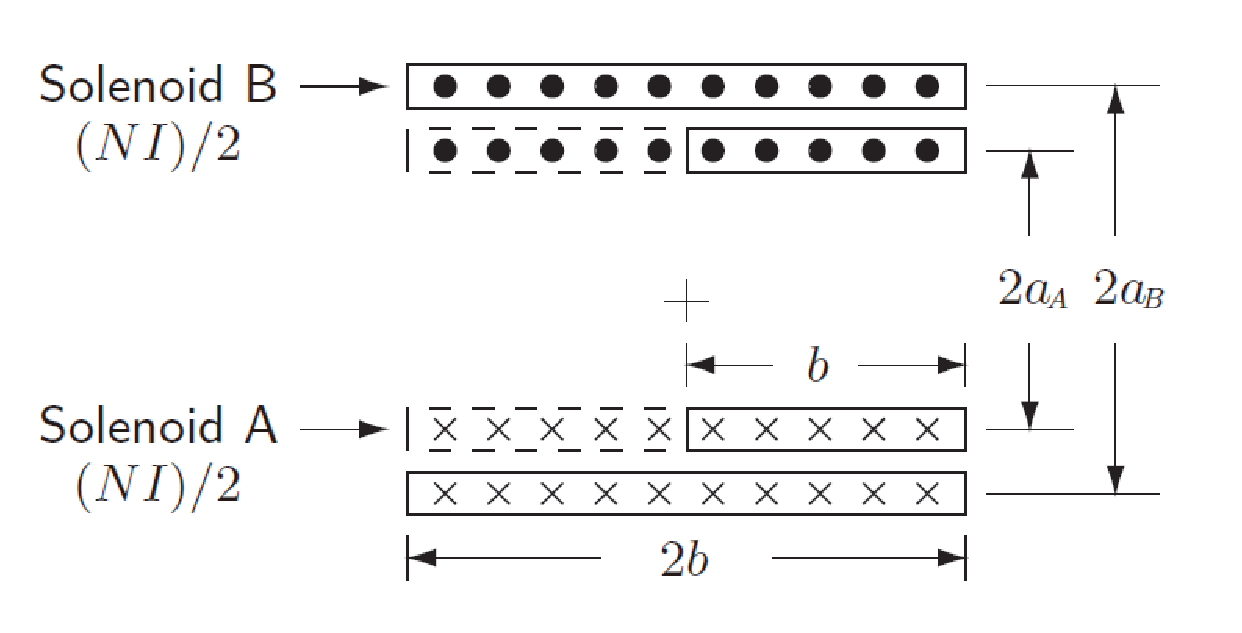
\includegraphics[scale=0.4]{chpt3/figs/fig3.8.eps}
  \caption{螺管线圈A和B的布置,用以计算线圈A上的中心面轴向力}
\end{figure}

于是,
\begin{equation}
\begin{split}
F_{zA}(0)=&-\frac{\mu_0}{2}(\frac{N I}{4b})\times \\
&( \{2b\sqrt{4a_A^2+b^2}[K(k_{b_A})-E(k_{b_A})]-2b\sqrt{4a_A^2+4b^2}[K(k_{2b_A})-E(k_{2b_A})]\}\\
&+\frac{2b}{\sqrt{a_T^2+b^2}} \{[a_T^2+b^2][K(k_{b})-E(k_{b})]-\Upsilon(c^2,k_b)\}\\
&-\frac{2b}{\sqrt{a_T^2+4b^2}} \{[a_T^2+4b^2][K(k_{2b})-E(k_{2b})]-\Upsilon(c^2,k_{2b}) \})
\end{split}
\end{equation}
其中,$c^2$已在3.47给出,模量为:
$$k_{b_A}^2=\frac{4a_A^2}{4a_A^2+b^2} ; k_{2b_A}^2=\frac{4a^2_A}{4a_A^2+4b^2} $$
$$k_{b_B}^2=\frac{4a_B^2}{4a_B^2+b^2} ; k_{2b_B}^2=\frac{4a^2_B}{4a_B^2+4b^2} $$

本例中,由于$2b_A=2b_B=2b$,$N_A I_A=N_B I_B$以及$F_{zAB}(0)=F_{zBA}(0)$,于是有:
\begin{equation*}
\begin{split}
F_{zB}(0)=&-\frac{\mu_0}{2}(\frac{N I}{4b})\times \\
&( \{2b\sqrt{4a_B^2+b^2}[K(k_{b_B})-E(k_{b_B})]-2b\sqrt{4a_B^2+4b^2}[K(k_{2b_B})-E(k_{2b_B})]\}\\
&+\frac{2b}{\sqrt{a_T^2+b^2}} \{[a_T^2+b^2][K(k_{b})-E(k_{b})]-\Upsilon(c^2,k_b)\}\\
&-\frac{2b}{\sqrt{a_T^2+4b^2}} \{[a_T^2+4b^2][K(k_{2b})-E(k_{2b})]-\Upsilon(c^2,k_{2b}) \})
\end{split}
\end{equation*}

螺管的总的中平面轴向力$F_{zT}(0)$分为两个薄壁线圈的各自受力$F_{zA}(0)$和$F_{zB}(0)$之和。于是我们得到:
\begin{equation}
\begin{split}
F_{zT}(0)=&-\frac{\mu_0}{2}(\frac{N I}{4b})\times \\
&( 2b\sqrt{4a_A^2+b^2}[K(k_{b_A})-E(k_{b_A})]-2b\sqrt{4a_A^2+4b^2}[K(k_{2b_A})-E(k_{2b_A})]\\
&+2b\sqrt{4a_B^2+b^2}[K(k_{b_B})-E(k_{b_B})]-2b\sqrt{4a_B^2+4b^2}[K(k_{2b_B})-E(k_{2b_B})]\\
&+\frac{4b}{\sqrt{a_T^2+b^2}} \{[a_T^2+b^2][K(k_{b})-E(k_{b})]-\Upsilon(c^2,k_b)\}\\
&-\frac{4b}{\sqrt{a_T^2+4b^2}} \{[a_T^2+4b^2][K(k_{2b})-E(k_{2b})]-\Upsilon(c^2,k_{2b}) \})
\end{split}
\end{equation}

当一个螺线圈被分为2个薄壁子螺管时,为获得$F_{zT}(0)$,要计算方程3.54中的4项;当一个螺线圈被分为$m>2$个薄壁螺管时,则要求计算$2(m!)/[(m−2)!]$项。比如$m=3$时,$F_{zT}(0)$的表达式中有12项,有18个模量,手算是很繁琐的。

为了编制可用来精确计算“实际”螺管线圈(“厚”壁)中平面轴向力的计算机代码,我们不得不按照m个薄壁线圈展开3.54。为了确保每一个子线圈是薄壁的,m可能是10或者更大。

注意到,多数情况下$c^2$是接近于1的,甚至对“长”螺管($\beta\gg 1$)也不可能近似$\prod(c^2,k)$项。

\subsubsection{特例9:长厚壁螺管的中平面力}
因为在大多数应用中,$c^2\simeq 1$,3.54中含$\prod{(c^2,k)}$项不能由其前几项近似表示。不过,3.54中的剩余项可以在$\beta \gg 1$时展开,正如特例5中所作的那样。于是,我们有:
\begin{equation}
\begin{split}
F_{zT}(0)\simeq& -\mu_0 (\frac{N I}{4b})^2\{ \pi(a_A^2+a_B^2)-(a_A^2-a_B^2)^2[2\prod(c^2,k_b)-\prod(c^2,k_{2b})]\}  \\
\simeq& -\mu_0 (\frac{N I}{4b})^2 \pi(a_A^2+a_B^2) \{ 1-\frac{(a_A^2-a_B^2)^2}{\pi(a_A^2+a_B^2)}[2\prod(c^2,k_b)-\prod(c^2,k_{2b})]\}
\end{split}
\end{equation}
可知,上式当$a_A=a_B$时,约化为3.41b式。在上式的第二行的形式中,大括号内的项可以视为修正项。

\subsection{嵌套双线圈磁体的轴向力}
在一个由多个轴向对齐的嵌套螺线管组成的磁体中,通常计算各个螺管的中平面轴向压缩力是很重要的;对于一个大型的嵌套螺管磁体,如MRI磁体,则更为重要。这里我们考虑最简单的仅有两个薄壁螺线管A和B组成的嵌套磁体,如图3.9所示。螺线管A(内)的参数为$2a_A,2b_A,N_A I_A/2b_A$;螺线管B(外)的参数为$2a_B, 2b_B, N_B I_B/2b_B$。
\subsubsection{施于A的中平面轴向力}
施于螺线管A右半部分的总中平面轴向力$F_{zA}(0)$是$F_{zAA}(0)$和$F_{zAB}(0)$之和。$F_{zAA}(0)$是其自身左半部分的中平面轴向力;$F_{zAB}(0)$来自螺线管B。$F_{zAA}(0)$可由方程3.41a替换下标A给出。 $F_{zAB}(0)$可由方程3.44采取如下替代得到: $b_A$替$2b_A$,$−(b_A+b_B)$替$\rho$,$2b_B$不变,$c^2$仍由3.47给出。
\begin{equation}
\begin{split}
F_{zA}(0)=&\frac{\mu_0}{2}[(\frac{N_A I_A}{2b_A})^2\times \\
&\{{2b_A\sqrt{4a_A^2+b_A^2}[K(k_{bA})-E(k_{bA})}]\\
&-2b_A\sqrt{4a_A^2+4b_A^2}[K(k_{2bA}-E(k_{2bA}]\}\\
&+(\frac{N_AI_A}{2b_A})(\frac{N_BI_B}{2b_B})(\frac{2b_B}{\sqrt{a_T^2+b_B^2}}\{[a_T^2+b_B^2][K(k_B)-E(k_{B})]-\Upsilon(c^2,k_B)\}\\
&-\frac{b_D}{\sqrt{a_T^2+b_D^2}}\{{[a_T^2+b_D^2][K(k_D)-E(k_D)]-\Upsilon(c^2,k_D)}\}\\
&-\frac{b_T}{\sqrt{a_T^2+b_T^2}}\{[a_T^2+b_T^2][K(k_T)-E(k_T)]-\Upsilon(c^2,k_T^2)\})]
\end{split}
\end{equation}

由$a_T=a_A+a_B$,$b_D=b_B-b_A$以及$b_T=b_A+b_B$,给出$k_{b_A}, k_{2b_A}, k_A,k_B, k_{AB}$:
$$ k_{bA}^2=\frac{4a_A^2}{4a_A^2+b_A^2}; k_{2bA}^2=\frac{4a_A^2}{4a_A^2+4b_A^2}; k_B^2=\frac{4a_Aa_B}{a_T^2+b_B^2};$$
$$k_D^2=\frac{4a_Aa_B}{a_T^2+b_D^2}; k_T^2=\frac{4a_Aa_b}{a_T^2+b_T^2}$$

\begin{figure}[htbp]
  \centering
 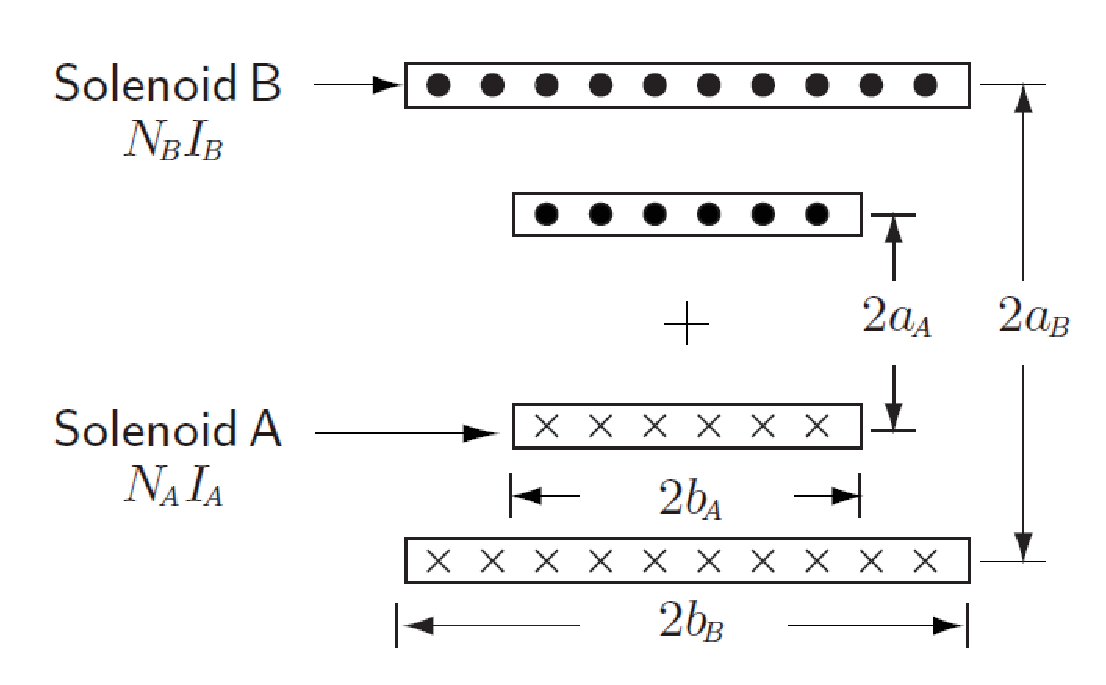
\includegraphics[scale=0.4]{chpt3/figs/fig3.9.eps}
  \caption{有螺管A和B组成的嵌套磁体}
\end{figure}

\subsubsection{特例10:长螺管的施于A的中平面力}
当两个螺线管都是“长”($b_A^2\gg 4a_A^2;b_B^2\gg a_T^2$)的,并且长度不一样,从而$b_D^2\gg a_T^2$,方程3.56可以简化为:
\begin{equation}
\begin{split}
F_{zA}(0)\simeq& -\frac{\mu_0}{2}\{(\frac{N_AI_A}{2b_A})^2\pi a_A^2+(\frac{N_AI_A}{2b_A})(\frac{N_BI_B}{2b_{B}})\times\\
&(a_A-a_B)^2[\Pi(c^2,k_D)+\Pi(c^2,k_T)-2\Pi(c^2,k_B)]]\}
\end{split}
\end{equation}

方程3.57a等号右侧的第二项代表$F_{zAB}$。物理上,这是由于螺线管B的磁场在螺线管A的接近螺线管B末端的轴向位置上的径向分量$B_r$引起的。注意到,当$b_A\rightarrow \infty$以及 $b_B\rightarrow \infty$时,第二项趋于。
\subsubsection{特例11:施于A的中平面轴向力——A和B均“长”但B比A更长}
当两个螺线管都如特例10中一样是“长”的,且B比A更长一些,也即$b_D\rightarrow b_B$以及$b_T\rightarrow b_B$时,方程3.57a可进一步化简为:
\begin{equation}
F_{zA}(0)\simeq F_{zAA}(0)\simeq -\frac{\mu_0}{2}(\frac{N_AI_A}{2b_A})^2\pi a_A^2
\end{equation}

物理上很容易理解,当$b_A/b_B\rightarrow 0$时有$F_{zAB}(0)\rightarrow 0$,因为螺管B比螺管A更长。作为$F_{zAB}(0)$中关键要素的螺管B的$B_r$在其室温孔内是0,而此处正式螺管A放置的位置。

\subsubsection{施于B上的中平面轴向力}
螺线管B的中平面上的轴向力的表达式与螺管A非常相似。我们可以通过变量替换的方式,直接从前几部分的方程得到。螺管B的中平面总轴向力$F_{zB}(0)$是$F_{zBB}(0)$与$F_{zBA}(0)$之和。其中,$F_{zBB}(0)$是由其自身左半部分产生的中平面轴向力,$F_{zBA}(0)$是螺线管A产生的。
\begin{equation}
\begin{split}
F_{zB}(0)=&-\frac{\mu_0}{2}[(\frac{N_BI_B}{2b_B})^2\times\\
&\{2b_B\sqrt{4a_B^2+b_B^2}[K(k_{bB})-E(k_{bB})]-2b_B\sqrt{4a_B^2+4b_B^2}[K(K_{2bB})-E(k_{2bB})]\}\\
&+(\frac{N_BI_B}{2b_B})(\frac{N_AI_A}{2b_A})(\frac{2b_A}{\sqrt{a_T^2+b_A^2}}\{[a_T^2+b_A^2][K(k_A)-E(k_A)]-\Upsilon(c^2,k_A)\}\\
&+\frac{b_D}{\sqrt{a_T^2+b_D^2}}\{[a_T^2+b_D^2][K(k_D)-E(k_D)]-\Upsilon(c^2,k_D)\}\\
&-\frac{b_T}{\sqrt{a_T^2+b_T^2}}\{[a_T^2+b_T^2][K(k_T)-E(k_T)]-\Upsilon(c^2,k_T)\})]
\end{split}
\end{equation}
式中的$c^2$同样有方程3.47给出,模量$k_{2b_B},k_A$如下给出:
\begin{equation}
k_{2bB}^2=\frac{a_B^2}{4a_B^2+4b_B^2};\quad \quad k_A^2=\frac{4a_Aa_B}{a_T^2+b_A^2}
\end{equation}
其他模量与方程3.56相同。

\subsubsection{特例12:施于B的中平面轴向力——A和B均“长”但B比A更长}
如特例11所述时,我们有:
\begin{equation}
\begin{split}
F_{zB}(0)\simeq&-\frac{\mu_0}{2}\{(\frac{N_BI_B}{2b_B})^2\pi a_B^2+(\frac {N_BI_B}{2b_B})(\frac{N_AI_A}{2b_A})[\pi(a_A^2+a_B^2)\\
&-(a_A-a_B)^2[2\Pi(c^2,k_A)+\Pi(c^2,k_D)-\Pi(c^2,k_T)]]\}
\end{split}
\end{equation}
如特例11中,方程3.59a中的第二项表示的$F_{zBA}$是可以忽略的,这是由于螺管A的$B_r$影响螺管A两端附近位置轴线上的螺管B。

\subsubsection{特例13:施于B的中平面轴向力——A和B均“长”但B比A短很多}
当两个螺管都是“长”的,但螺管B比螺管A短很多($b_D^2\rightarrow b_A^2\gg a_T^2$)时,方程3.58简化为:
\begin{equation}
F_{zB}(0)\simeq-\frac{\mu_0}{2}(\frac{N_BI_B}{2b_B})^2\pi a_B^2
\end{equation}

方程3.59b可以类比为特例11中的3.57b。也可以用相同的物理原因解释这个结果。

\subsection{轴向偏心螺管的轴向恢复力}
当每一个螺管的轴向场都是指向同一个方向并且螺管A和螺管B的轴中心失配距离为$\rho$时,将产生一个轴向恢复力$F_{zR}(\rho)$以对齐轴中心。$F_{zR}(\rho)$可以写为:
\begin{equation}
\begin{split}
F_{zR}(\rho)=&-\frac{\mu_0}{2}(\frac{N_AI_A}{2b_A})(\frac{N_BI_B}{2b_B})\times\\
&(\frac{b_T-\rho}{\sqrt{a_T^2+(b_T-\rho)^2}}\{[a_T^2+(b_T-\rho)^2][K(k_{T-})-E(k_{T-})]-\Upsilon(c^2,k_{T-})\}\\
&+\frac{b_D+\rho}{\sqrt{a_T^2+(b_T+\rho)^2}}\{[a_T^2+(b_D+\rho)^2][K(k_{D+})-E(k_{D+})]-\Upsilon(c^2,k_{D+})\}\\
&-\frac{b_T+\rho}{\sqrt{a_T^2+(b_T+\rho)^2}}\{[a_T^2+(b_T+\rho)^2][K(k_{T+})-E(k_{T+})]-\Upsilon(c^2,k_{T+})\}\\
&-\frac{b_D-\rho}{\sqrt{a_T^2+(b_D-\rho)^2}}\{[a_T^2+(b_D-\rho)^2][K(k_{D-})-E(k_{D-})]-\Upsilon(c^2,k_{D-})\})
\end{split}
\end{equation}
式中,$a_T=a_A+a_B, b_T=b_A+b_B, b_D=b_A−b_B$。模量:
\begin{eqnarray}
k_{T+}^2&=&\frac{4a_Aa_B}{a_T^2+(b_T+\rho)^2}; k_{T-}^2=\frac{4a_Aa_B}{a_T^2+(b_T-\rho)^2}\\ \nonumber
k_{D+}^2&=&\frac{4a_Aa_B}{a_T^2+(b_D+\rho)^2};  k_{D-}^2=\frac{4a_Aa_B}{a_T^2+(b_D-\rho)^2}
\end{eqnarray}

\subsubsection{特例14:不存在轴向失配}
当$\rho=0, k_{T+}^2=k_{T-}^2, k_{D+}^2=k_{D-}^2$时,有$F_{zR}(\rho)=0$。这和物理上的预期是一致的。

\subsubsection{特例15:微小的轴向失配}
对于很小的失配,规定为$\rho\ll \sqrt{a_T^2+b_D^2}$,$F_{ZR}(\rho)$正比于$\rho$:
\begin{equation}
F_{zR}(\rho)\propto-(\frac{N_AI_A}{2b_A})(\frac{N_BI_B}{2b_B})\rho
\end{equation}

方程3.61后面将用来推导小失配距离线圈A和B之间的互感表达式$M_{AB}(\rho)$。

\subsubsection{特例16:某一螺管是“长”的}
如果螺管A或螺管B之一是“长”的,这个更长的螺管的轴向场将成为均匀的,其$B_r$就很小了,哪怕两个线圈之间存在可观的失配,长螺管在短线圈上也只产生很小的轴向力。方程3.60在$b^2_T\gg a_T^2,b_D^2\gg a_T^2$时前两个+项和后两个-项抵消,有$F_{zR}(\rho)\rightarrow 0$。

\section{螺管在磁力下的应力应变}
此处研究超导体在(主要是)洛伦兹力的应力和应变。本节的磁应力的分析解和图表都是在简单场分布下的应用绕组材料的简单性质而得到的。

\subsection{应力应变方程}
处于由轴向磁场$B_z(r,z)$和电流$\lambda J$相互作用产生的磁场力下的螺管绕组的应力(径向$\sigma_r(r,z)$,环向$\sigma_\theta(r,z)$,轴向$\sigma_z(r,z)$,剪切$\tau_{rz}(r,z)$)满足以下平衡方程:
\begin{eqnarray}
\frac{\partial\sigma_{r}}{\partial_r}+\frac{\sigma_{r}-\sigma_{\theta}}{r}+\frac{\partial \tau_{rz}}{\partial z}&=&-\lambda JB_z(r,z)\\
\frac{\partial \tau_{rz}}{\partial r}-\frac{\tau_{rz}}{r}+\frac{\partial \sigma_z}{\partial_z}&=&-\lambda JB_r(r,z)
\end{eqnarray}

边界条件为:$\sigma_r(r=a_1,z);\sigma_r(r=a_2,z);\sigma_z(r,z=\pm b)=0;\tau_{rz}(r=a_1,z)=0;\tau_{rz}(r=a_2,z)=0;\tau_{rz}(r,z=\pm b)=0$。
注意到剪切力是方程3.62a和3.62b中唯一的变量。大多数复合超导体,包括LTS和HTS,都可以视为正交各向异性:可以应用Hooke定律。正交各向异性材料具有以下机械性质:Young模量,Poisson比。它们在三个正交方向不同,但都关于正交方向对称。应变$\epsilon_r,\epsilon_\theta,\epsilon_z$分别为$r,\theta,z$向,剪切应变$\gamma_{rz}$位于$r-z$平面。应变关系:
\begin{eqnarray}
\epsilon_r&=&\frac{1}{E_r}\sigma_r-\frac{\nu_{\theta r}}{E_{\theta}}\sigma_{\theta}-\frac{\nu_{zr}}{E_z}\sigma_z+\epsilon_{Tz}\\
\epsilon_\theta&=&-\frac{\nu_{r\theta}}{E_r}\sigma_r+\frac{1}{E_{\theta}}\sigma_{\theta}-\frac{\nu_{z\theta}}{E_z}\sigma_z+\epsilon_{T\theta}\\
\epsilon_z&=&-\frac{\nu_{rz}}{E_r}\sigma_r-\frac{\nu_{\theta z}}{E_{\theta}}\sigma_{\theta}+\frac{1}{E_z}\sigma_z+\epsilon_{Tz}\\
\gamma_{rz}&=&\frac{1}{G_{{rz}}}\tau_{rz}
\end{eqnarray}

$E_r, E_\theta, E_z$分别是各向的Young模量。$\mu_{12}\equiv -\epsilon_2/\epsilon_1$,当材料应力加在1方向时($\sigma_1;\sigma_2=\sigma_3=0$)两个正交方向的横向应变的Poisson比。$G_{rz}$是剪切模量。 
$\epsilon_{Tr},\epsilon_{T\theta},\epsilon_{Tz}$分别为从室温$300\ \mathrm{K}$到运行温度$T_{op}$的热膨胀积分系数。
\begin{eqnarray}
\epsilon_{T_r}&=&\int_{300K}^{T_{op}}\alpha_{Tr}(T)dT;\\ \nonumber
\epsilon_{T_\theta}&=&\int_{300K}^{T_{op}}\alpha_{T_\theta}(T)dT;\\ \nonumber
 \epsilon_{T_Z}&=&\int_{300k}^{T_{op}}\alpha_{Tz}(T)dT
\end{eqnarray}

$\alpha_{Tr}(T),\alpha_{T\theta}(T),\alpha_{Tz}(T)$分别为平行于各自主轴的热膨胀系数,与温度有关。
注意到这些系数是正的,并且因为是从$300\ \mathrm{K}$到度$T_{op}<300\ \mathrm{K}$积分,方程3.63a-3.63c中的热应变是负的,也即压缩力。

应用下列$\nu$和$E$的关系:
\begin{equation}
\frac{\nu_{r\theta}}{E_\theta}=\frac{\nu_{\theta r}}{E_r};\quad \frac{\nu_{\theta z}}{E_z}=\frac{\nu_{z\theta}}{E_\theta};\quad \frac{\nu_{zr}}{E_r}=\frac{\nu_{rz}}{E_z}
\end{equation}

在轴对称体情况下,例如理想螺线管,在r和z方向的应变$u_r$和位移$u_z$分别为:
\begin{equation}
\epsilon_r=\frac{\partial_{u_r}}{\partial_r};\quad \epsilon_\theta=\frac{u_r}{r};\quad \epsilon_z=\frac{\partial_{u_z}}{\partial_z};\quad \gamma_{rz}=\frac{\partial_{u_r}}{\partial_z}+\frac{\partial_{u_z}}{\partial_r}
\end{equation}

由于轴对称,方程3.62中的所有变量都与$\theta$无关,且有$u_\theta=0$。一般的,不同时存在$\sigma_r$和$\sigma_z$的闭式解。在一个“长”螺管中,例如多用于空间高磁场均匀性NMR磁体的螺管中,$B_z(r, z)$在z方向至少是在螺管以中平面为起点的很大长度内的变化都是很小的。剪切应力$\tau_{rz}$是由$B_z(r,z)$在线圈上产生的径向载荷的变化导致的。因此,在一个长螺管中,我们可以假设所有变量不依赖于z(包括$u_r$,有$\partial u_r/\partial z=0$)来化简3.62a。因为在高磁场均匀性磁体中有$\partial B_r(r,z).\partial z\simeq 0$,我们可以放心的假设在磁体轴向的大部分长度上有$\partial u_r/\partial z=0$成立。加上$\partial u_z/\partial r=0$,我们发现$\gamma_{rz}=\tau_{rz}=0$。反过来,这个结果 有会解耦3.62a和3.62b。

联立方程3.62和3.63,假设$\tau_{rz}=0$,用$u_r$解出$\sigma_r$和$\sigma_{\theta}$,我们得到以下微分方程:
\begin{equation}
\frac{d^2u_r}{d_r^2}+\frac{1}{r}\frac{du_r}{dr}-\zeta^2\frac{u_r}{r^2}=-\frac{1-\nu_{r\theta}\nu_{\theta r}}{E_r}\lambda JB_z(r)+\frac{F}{r}
\end{equation}

式中,
\begin{equation}
\zeta=\sqrt{\frac{E_\theta}{E_r}};\quad F=
-(\zeta^2-\nu_{r \theta})\epsilon_{T_\theta}+(1-\nu_{\theta r}\zeta^2)\epsilon_{Tr}
\end{equation}

方程3.64a的解的一般形式:
\begin{equation}
u_r=C_1r^\zeta+\frac{C_2}{r^\zeta}+u_r^L+u_r^T
\end{equation}

式中,$C_1,C_2$是由$r = a_1, r = a_2$边界条件确定的常数。
$u^L_r$和$u^T_r$ (上标L和T分别代表Lorentz和thermal) 依赖于方程3.64a等式右侧源项的特解。
热学项$u^T_r$为:
\begin{equation}
u_r^T=\frac{Fr}{1-\zeta^2}
\end{equation}

对各向同性材料($E_\theta =E_r,\zeta =1$),$u_r^T$为:
\begin{equation}
u_r^T(\zeta=1)=\frac{1}{2}Fr \ln r
\end{equation}

一般的,$B_z(r)$可以用幂级数给出:
\begin{equation}
B_z(r)=\sum_{k=0}^{n}b_kr^k
\end{equation}

于是,Lorentz项可以表示为:
\begin{equation}
u_r^T=\frac{1-\nu_{r\theta}\nu_{\theta r}}{E_r}\lambda J\sum_{k=0}^{n}\frac{b_k r^{k+2}}{\zeta^2-(k+2)^2}
\end{equation}

\subsection{各向同性螺管的应力应变方程}
本节我们推导具有绕组电流密度$\lambda J$的各向同性螺线管径向和方位角方向的应力。
绕组中的轴向场从$B_z(r = a_1)\equiv B_1$到$B_z(r = a_2)\equiv B_2$随r线性变化。
注意到在嵌套线圈磁体中,$B_1,B_2$都可能包括由位于外部的“长”线圈产生的不均匀背景场。
我们定义两个无量纲参数:$\kappa\equiv B_2/B_1,\rho = r/a_1$。在一个高场NMR磁体中,最内部的线圈$\kappa$会超过0.9;对一个孤立的线圈,大概是-0.1;对于无限长孤立线圈,有$\kappa=0$。于是,方程3.62a可以修正为:
\begin{equation}
\frac{d\sigma_{\rho}}{d\rho}+\frac{\sigma_\rho-\sigma_\theta}{\rho}=-\frac{\lambda JB_1a_1}{\alpha-1}[\alpha-\kappa-(1-\kappa)\rho]
\end{equation}

对于各向同性材料,考虑热应变$\epsilon_T$的应变为:
\begin{eqnarray}
\epsilon_\rho&=&\frac{1}{E}(\sigma_\rho-\nu\sigma_\theta)+\epsilon_T\\
\epsilon_\theta&=&\frac{1}{E}(\sigma_\theta-\nu\sigma_\rho)+\epsilon_T
\end{eqnarray}

从上式中解出$\sigma_\rho,\sigma_{\theta}$:
\begin{eqnarray}
\sigma_\rho&=&\frac{E}{1-\nu^2}[\epsilon_\rho+\nu\epsilon_\theta-(1+\nu)\epsilon_T]\\
\sigma_\theta&=&\frac{E}{1-\nu^2}[\epsilon_\theta+\nu\epsilon_\rho-(1+\nu)\epsilon_T]
\end{eqnarray}

应变是和位移$u$有关的:
\begin{equation}
\epsilon_\rho=\frac{1}{a_1}\frac{du}{d\rho};\quad \epsilon_\theta=\frac{1}{a_1}\frac{u}{\rho}
\end{equation}

联立3.72a-3.72c,我们得到:
\begin{eqnarray}
\sigma_\rho&=&\frac{E}{(1-\nu^2)a_1}[\frac{du}{d\rho}+\nu\frac{u}{\rho}-a_1(1+\nu)\epsilon_T]\\
\sigma_\theta&=&\frac{E}{(1-\nu^2)a_1}[\frac{u}{\rho}+\nu\frac{du}{d\rho}-a_1(1+\nu)\epsilon_T]
\end{eqnarray}

联立3.70和方程3.92d,3.72e,得到:
\begin{equation}
\frac{d^2u}{d\rho^2}+\frac{1}{\rho}\frac{du}{d\rho}-\frac{u}{\rho^2}=-(\frac{1-\nu^2}{E})(\frac{\lambda JB_1a_1^2}{\alpha-1})[\alpha-\kappa-(1-\kappa)\rho] %(3.73)
\end{equation}

方程3.73的通解为:
\begin{equation}
u=C_1\rho+\frac{C_2}{\rho}-(\frac{1-\nu^2}{E})(\frac{\lambda JB_1a_1^2}{\alpha-1})[\frac{(\alpha-\kappa)\rho^2}{3}-\frac{(1-\kappa)\rho^3}{8}]%\(3.74)
\end{equation}

式中,$C_1,C_2$是由$\rho=1$和$\rho=\alpha$处的边界条件确定的常数;最后一项是特解。联立3.74,3.72d和3.72e,我们得到:
\begin{eqnarray}
\sigma_\rho&=&\frac{E}{(1-\nu^2)a_1}\left[(1+\nu)C_1-(1-\nu)\frac{C_2}{\rho^2}\right] \\ \nonumber
&-&\left\{\frac{\lambda JB_1a_1}{\alpha-1}[\frac{2+\nu}{3}(\alpha-\kappa)\rho-\frac{3+\nu}{8}(1-\kappa)\rho^2]\right\}-\frac{E\epsilon_T}{1-\nu}\\
\sigma_\theta&=&\frac{E}{(1-\nu^2)a_1}\left[(1+\nu)C_1+(1-\nu)\frac{C_2}{\rho^2}\right]\\ \nonumber
&-&\left\{\frac{\lambda JB_1\alpha_1}{\alpha-1}[\frac{1+2\nu}{3}(\alpha-\kappa)\rho-\frac{1+3\nu}{8}(1-\kappa)\rho^2]\right\}-\frac{E\epsilon_T}{1-\nu}
\end{eqnarray}

代入$\sigma_{\rho}(1)=0$和$\sigma_{\rho}(\alpha)=0$,我们得到$C_1,C_2$的表达式:
\begin{eqnarray}
{[(1+\nu)C_1-(1-\nu)C_2]}&=&\frac{1-\nu^2}{E}(\frac{\lambda JB_1a_1^2}{\alpha-1})  \\ \nonumber
&\times&\left[\frac{2+\nu}{3}(\alpha-\kappa)-\frac{3+\nu}{8}(1-\kappa)\right]+a_1(1+\nu)\epsilon_T\\
{[(1+\nu)C_1-(1-\nu)\frac{C_2}{\alpha^2}]}&=&\frac{1-\nu^2}{E}(\frac{\lambda JB_1a_1^2}{\alpha-1})  \\ \nonumber
&\times&\left[\frac{2+\nu}{3}(\alpha-\kappa)\alpha-\frac{3+\nu}{8}(1-\kappa)\alpha^2\right] +a_1(1+\nu)\epsilon_T %3.76a 3.76b
\end{eqnarray}

解出$C_1,C_2$:
\begin{eqnarray}
C_1&=&\frac{1-\nu}{E}(\frac{\lambda JB_1a_1^2}{\alpha^2-1}) \\ \nonumber
&\times&\left[\frac{2+\nu}{3}(\alpha-\kappa)(\alpha^2+\alpha+1)-\frac{3+\nu}{8}(1-\kappa)(\alpha+1)(\alpha^2+1)\right] +a_1\epsilon_T\\
C_2&=&\frac{1+\nu}{E}(\frac{\lambda JB_1a_1\alpha^2}{\alpha^2-1})\\ \nonumber
&\times &\left[\frac{2+\nu}{3}(\alpha-\kappa)-\frac{3+\nu}{8}(1-\kappa)(\alpha+1)\right]
\end{eqnarray}

将方程3.76c和3.76d代入3.75,我们可以得到:
\begin{eqnarray}
\sigma_\rho&=&\frac{\lambda JB_1a_1}{\alpha-1}[\frac{2+\nu}{3}(\alpha-\kappa)(\frac{\alpha^2+\alpha+1-\frac{\alpha^2}{\rho^2}}{\alpha+1}-\rho) \\ \nonumber
&-&\frac{3+\nu}{8}(1+\kappa)(\alpha^2+1-\frac{\alpha^2}{\rho^2}-\rho^2)]\\
\sigma_\theta&=&\frac{\lambda JB_1a_1}{\alpha-1}\{(\alpha-\kappa)[\frac{2+\nu}{3}(\frac{\alpha^2+\alpha+1+{\frac{\alpha^2}{\rho^2}}}{\alpha+1})-\frac{1+2\nu}{3}\rho] \\ \nonumber
&-&(1-\kappa)[\frac{3+\nu}{8}(\alpha^2+1+\frac{\alpha^2}{\rho^2})-\frac{1+3\nu}{8}\rho^2]\}
\end{eqnarray}

\subsubsection{薄壁线圈}
图3.10a和3.10b分别画出了薄壁线圈(这里$\alpha=1.2$)的归一化方位角向应力($\varsigma_\theta\equiv \sigma_{\theta}/(\lambda J B_1 a_1)$)和径向应力($\varsigma_r\equiv \sigma_{\rho}/(\lambda J B_1 a_1)$)与归一化径向距离($\rho\equiv r/a_1$ )在几个特定的“场比率”($\kappa\equiv B_2/B_1$)下的关系。
我们发现,$\kappa=-0.1$对应孤立螺管;$\kappa=0$对应无限长线圈;$\kappa>0$对应处于均匀背景场中的线圈。
\begin{figure}
  \centering
 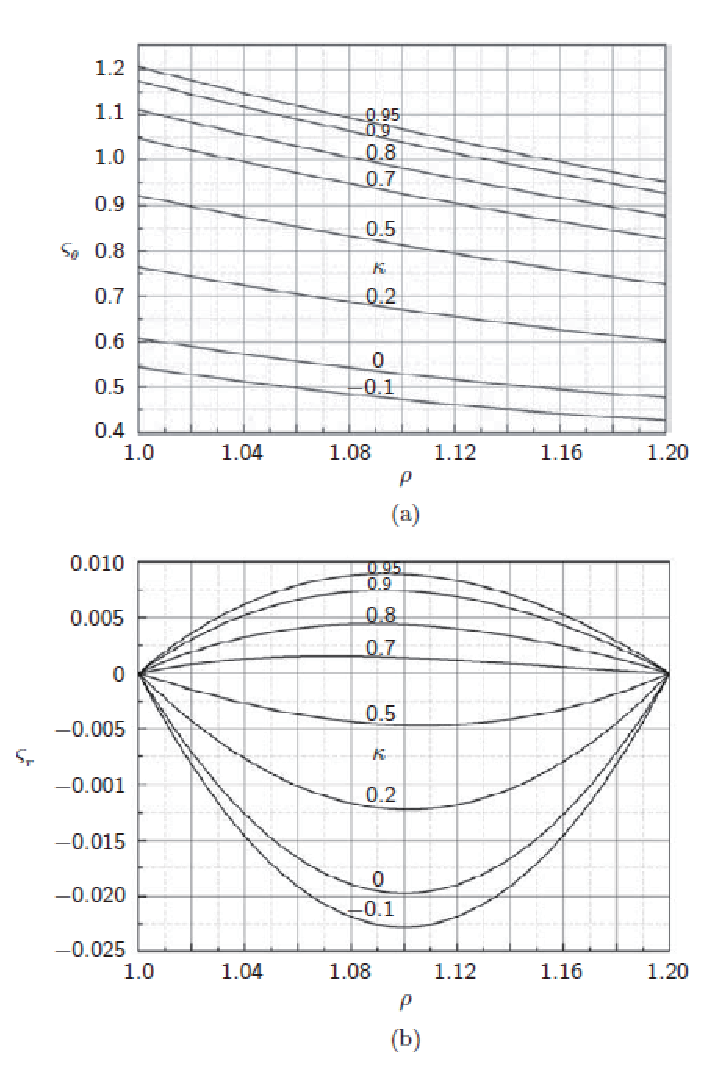
\includegraphics[scale=0.8]{chpt3/figs/fig3.10.eps}
  \caption{几个$\kappa\equiv B_2/B_1$值下的薄壁线圈($\alpha=1.2$)的特性图:a)归一化切应力$\varsigma_\theta\equiv \sigma_\theta/(\lambda J B_A a_1)$ vs. 归一化径向距离$\rho\equiv r/a_1$;
  b)归一化径向应力$\varsigma_r \equiv \sigma_\rho/(\lambda J B_A a_1)$ vs. $\rho$。各图中,$\kappa$的取值均为-0.1(最下);0;0.2;0.5;0.7;0.8;0.9;0.95(最顶) }
\end{figure}

对于$\kappa>0.5$,绕组总体上有一个正的径向应力,倾向于将各匝分开。这种情况一般是要避免的。

\subsubsection{中等厚度线圈}
图3.11给出了“中等厚度”线圈($\alpha=1.8$)的类似于图3.10的特性。这里,$\alpha=1.8$。
在这个中等厚度线圈中,在$\kappa\simeq 0.2$时有$\varsigma>0$;在$\kappa> 0.8$时$\varsigma$超过0.1。也即,一个内插入高场背景场磁体室温孔中的线圈应当是薄壁的,不然,它应当被切分为多个薄壁的。

\begin{figure}
  \centering
 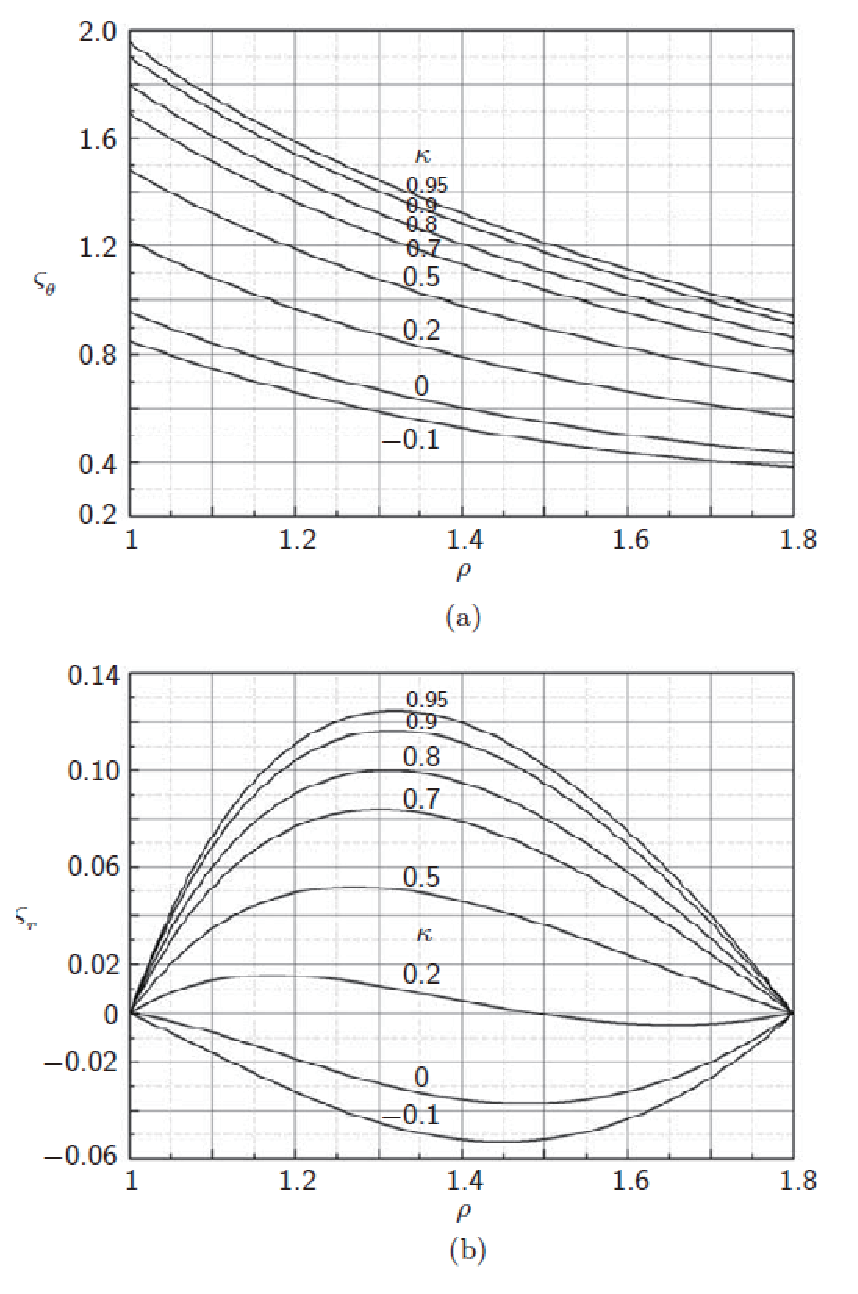
\includegraphics[scale=0.7]{chpt3/figs/fig3.11.eps}
  \caption{几个$\kappa\equiv B_2/B_1$值下的中等厚度线圈($\alpha=1.8$)的特性图:a)$\varsigma_\theta\equiv \sigma_\theta/(\lambda J B_A a_1)$ vs.$\rho$;
  b)$\varsigma_r \equiv \sigma_\rho/(\lambda J B_A a_1)$ vs. $\rho$。各图中,$\kappa$的取值均为-0.1(最下);0;0.2;0.5;0.7;0.8;0.9;0.95(最顶) }
\end{figure}

\subsubsection{厚壁线圈}
类似的,图3.12给出了厚壁线圈($\alpha=3.6$)的特性图,这里$\alpha=3.6$。注意到,$\varsigma_\theta$大致是中等厚度线圈的2倍。最显著的是,厚壁线圈的归一化径向应力只在$\kappa$明显小于0时才为正值。
有两种实用方法可以令$\sigma_{r}$接近0或者成为负值:1) 预应力绕制线圈;2)在最外层用绑线或高弹性模量材料绑扎。同时,将线圈分割为更薄的线圈不仅降低$\sigma_{r}$还降低$\sigma_{\theta}$。
\begin{figure}
  \centering
 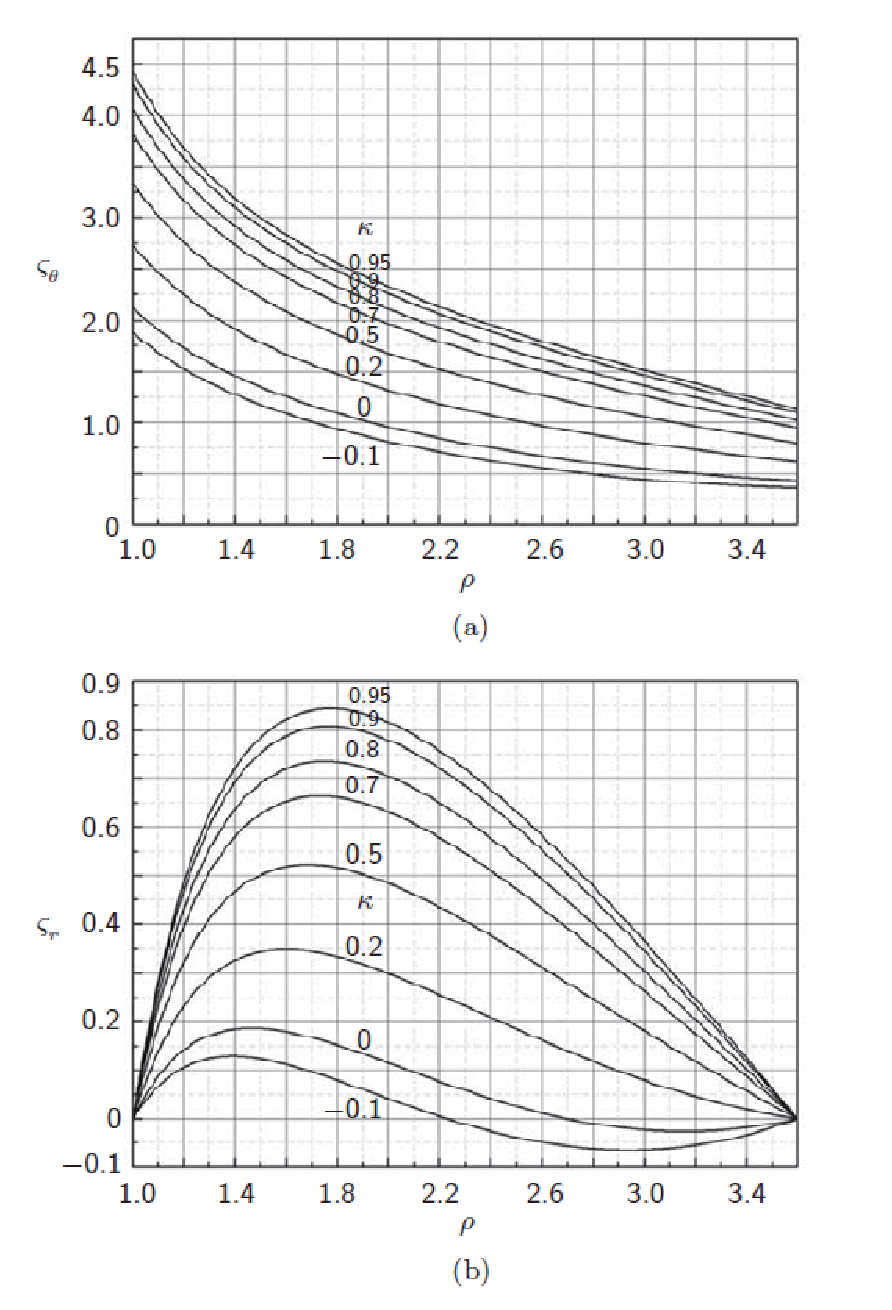
\includegraphics[scale=0.7]{chpt3/figs/fig3.12.eps}
  \caption{几个$\kappa\equiv B_2/B_1$值下的中厚壁线圈($\alpha=3.6$)的特性图:a)$\varsigma_\theta\equiv \sigma_\theta/(\lambda J B_A a_1)$ vs.$\rho$;
  b)$\varsigma_r \equiv \sigma_\rho/(\lambda J B_A a_1)$ vs. $\rho$。各图中,$\kappa$的取值均为-0.1(最下);0;0.2;0.5;0.7;0.8;0.9;0.95(最顶) }
\end{figure}


\subsection{减小径向应力的绕制张力}
这里用一个例子演示绕组张力对减小径向应力$\sigma_{r}$的好处。如上文所述,$\sigma_{r}$在绕组中应当保持负值以保证各层不再径向分离。简单来说,当线圈是由预张力导体绕成时,张力产生径向的向内应力,减少了绕组内部的径向应力。尽管绕组张力在绕制过程中维持恒定,张力效应在绕组内的径向变化也很难写出为磁力的近似表达式。由于绕组张力的存在,绕向角向和径向的应力计算必须通过数值分析得到。

考虑一个放置于高场背景磁体室温孔内的线圈。插入线圈的参数为内径$2a_1=87 mm$,外径$2a_2=156.6 mm$,即$\alpha = 1.8$:这是一个中等厚度磁体。我们假设线圈是“长”的。插入线圈的其他参数包括:
$B_z(r=a_1)\equiv B_1 =28.1 T; B_z(r=a_2)\equiv B_2 =24.3 T;\kappa\equiv B_2/B_1 = 0.865; \lambda J =8.26×10^7 A/m^2$。从图3.11的$\varsigma_r(\rho)$在$\alpha=1.8$时的曲线,我们找到归一化径向应力的最大值时0.11,在$\rho=r/a_1=1.3$时取得。于是,最大径向应力为:
\begin{equation}
  [\sigma_r]_{mx}=0.11\lambda JB_1\alpha_1  =0.11(8.26\times 10^7 A/m^2)(28.1T)(43.5\times10^{-3}m)=11.1MPa%page105
\end{equation}

11.1MPa的径向应力在内插线圈内是难以承受的。图3.13给出了在几个给定绕制张力下(从0到最大$200 N\simeq 20 kg$)的$\sigma_{r}$和r的关系。本图说明,绕制张力至少要求160 N才能保证$\sigma_{r}$为0或为负值。
实践中,可能应用大到200N的张力来绕线圈。对于这个特别的内插磁体,绕制张力80N时,最大应力减小至大约5MPa。当线圈是用环氧浸渍时,正的径向5MPa应力是可以承受的。
\begin{figure}[htbp]
  \centering
 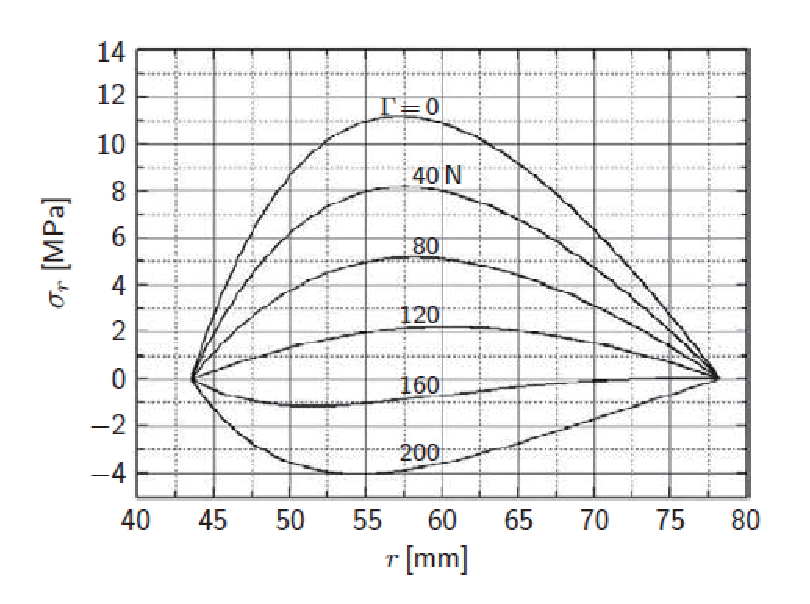
\includegraphics[scale=0.7]{chpt3/figs/fig3.13.eps}
  \caption{$\alpha=1.8$的螺管线圈在不同张力$\Gamma$下的$\sigma_r$ vs. r。$\Gamma=0$时,$\sigma$取得峰值,在$r\simeq 57.5 mm$处约为11.1MPa。
  当张力大于160N($\simeq 16 kg$)后,处处$\sigma_r\le 0 $。}
\end{figure}




%%%%%%%%%%%%%%%%%% 第3.7节%%%%%%%%%%%%%%%%%%%%%%
\section{自感}
线圈的总磁链$\Phi$正比于通过线圈的电流$I$:
\begin{equation}
 \Phi=LI %page106
\end{equation}

比例系数$L$是线圈的自感。注意到$\Phi$是一个“场”量概念,而$I$是一个“路”量概念:$L$将这两个概念连接起来。
因为“场”的概念必然涉及体积,故$L$是一个与几何有关的量。$L$还与线圈中存储的磁能$E_m$有关:
\begin{equation}
 E_m=\frac{1}{2}LI^2 %page106
\end{equation}
对于不含有磁性材料的系统,$E_m$可通过在整个空间积分$(1/2)\mu_0 H^2$计算。可见,$E_m$是另一个“场”量概念;$L$通过方程3.79将$E_m$和$I$连接在一起。

\subsection{圆形闭合回路的自感}
一根半径为$a$、磁导率为$\mu$的导线围成的半径为$R$的圆环的$L$公式可由Maxwell方程导出:
\begin{eqnarray}
L&=&\mu_0R[ln(\frac{8R}{a}-2)]+\frac{1}{4}\mu R \\
&\simeq & \mu_0R[ln(\frac{R}{a})+0.079]+\frac{1}{4}\mu R%page106
\end{eqnarray}

上述方程的等号右侧,第一项是由圆环内部区域$(0\le r \le R-a)$磁通贡献的自感;第二项由是$2\pi R$长的导线内部贡献的自感圆环自感(问题3.18)。因为导线外部的磁链与频率无关,第一项对所有频率都成立,而第二项是频率相关的。$(1/4)\mu R$仅对低频成立;第二项在高频时趋向于零。第一项的推导是非常复杂的,涉及到椭圆积分等高等数学。

\subsection{螺管线圈的自感}
对于一个不含有铁磁材料,由绕组内径$a_1,\alpha,\beta$以及总匝数$N$确定的螺管线圈的自感$L$可以写为:
\begin{equation}
L=\mu_0a_1N^2L(\alpha,\beta)%page107
\end{equation}

式中,$L(\alpha,\beta)$是一个无量纲电感参数,仅与由$\alpha,\beta$表示的线圈形状有关。图3.14画出了我们感兴趣的$\alpha=1$至$\alpha=5$,$\beta=0.04$至$\beta=10$范围内的$L(\alpha,\beta)$。
$\beta>1$涵盖了大部分螺管线圈,但“环”和“饼”是重要的例外。如图中所示,$L(\alpha,\beta)$大致上正比于$\alpha$。事实上,当一个粗略的("ball-park")$L$值足够时,例如在“first-cut”设计阶段,我们可以使用:
\begin{eqnarray}
\mathcal{L}(\alpha,\beta)&\sim&\frac{\pi\alpha}{2(\beta+0.5)} (for \beta\rightarrow 1 from \beta>1)\\ %\text{(for\rightarrow1 from\beta>1)}\\%page107
\mathcal{L}(\alpha,\beta)&\sim&\frac{\pi\alpha}{2\beta} (for \beta\rightarrow \infty)%\text{(for\beta\rightarrow\infty)}%page107
\end{eqnarray}

\begin{figure}[htbp]
  \centering
 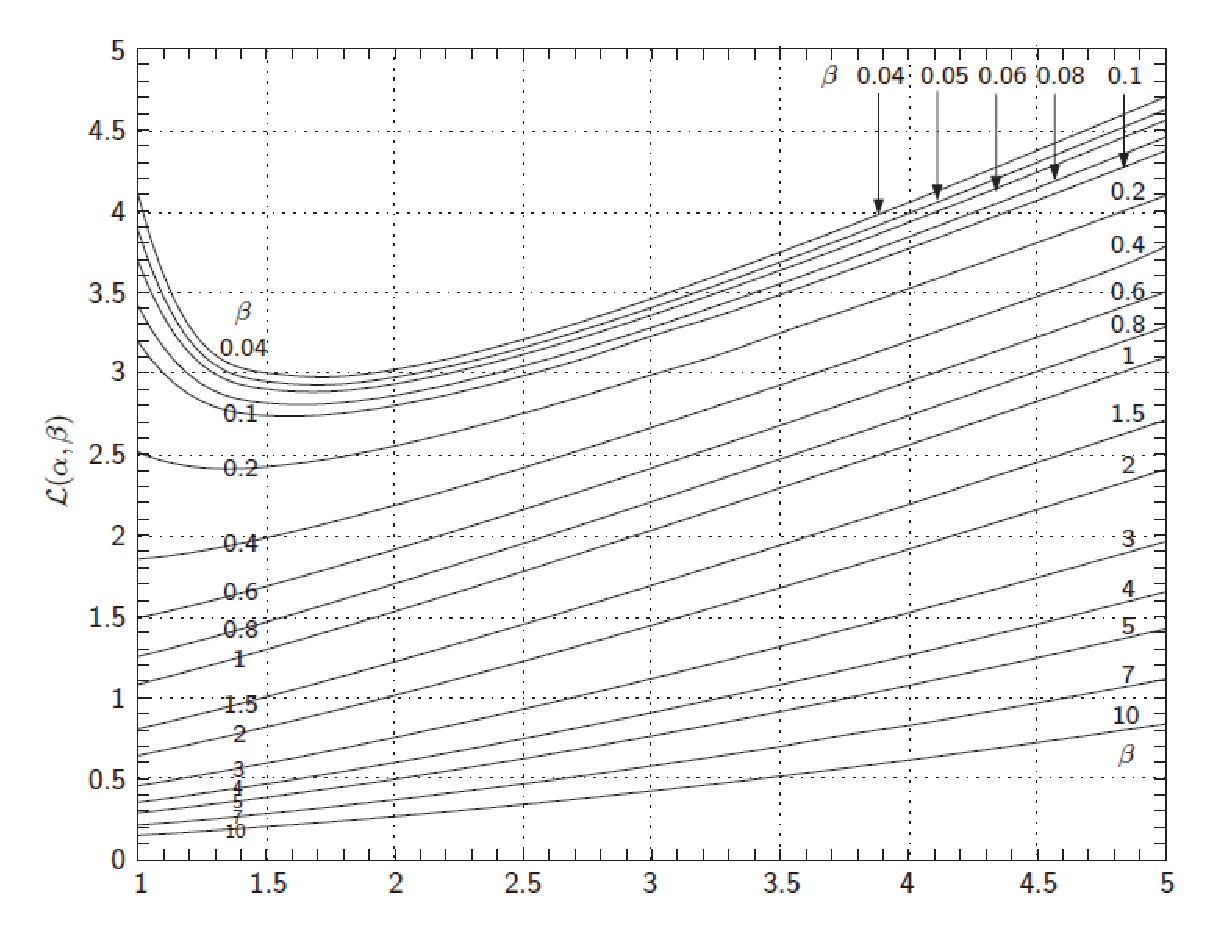
\includegraphics[scale=0.5]{chpt3/figs/fig3.14.eps}
  \caption{参数$\alpha,\beta$下的$\mathcal{L}(\alpha,\beta)$}
\end{figure}

对于一个“薄壁”螺管,即$\alpha\simeq 1,\beta\rightarrow \infty$,3.82b简化为$\pi/2\beta$(问题3.18)。

\subsection{实用电感公式}
本节给出非磁性材料($\mu=\mu_0$)线圈的电感公式。一些公式的推导,在问题3.18中会再次涉及。

尽管过去——电感计算程序大量使用之前——推导出了“厚”线圈的解析表达式并写入工程参考书中,这些公式一般来说是很难用的。图3.14,甚至方程3.82,对大多数应用,特别是早期设计的电感计算足够了。


\textbf{导线}  
  
  半径为$a$的导线单位长度电感$L[H/m]$为:
  \begin{equation}
         L=\frac{\mu_0}{8\pi}%page108
  \end{equation}
  
\textbf{“长”线圈} 
  
  a. 一个“长”$(β>0.75)$、“薄”($2a_1$)、$N$匝的线圈:
  \begin{equation}
  L=\mu_0a_1N^2[\frac{\pi(1+\alpha)^2}{8\beta}][1-\frac{2}{3\pi\beta}+\frac{(1+\alpha)^2}{32\beta^2}...]%page108
\end{equation}

在$(\alpha−1)/(\alpha+1)\ll 1$时,化简为:
\begin{equation}
  L=\mu_0a_1N^2(\frac{\pi}{2\beta})[1-\frac{2}{3\pi\beta}+\frac{1}{8\beta^2}...]%page108
\end{equation}

b.一个“很长”($\beta\gg 1$)、“薄”($\alpha \simeq 1$),方程3.84b成为:
\begin{equation}
  L=\mu_0a_1N^2(\frac{\pi}{2\beta})%page108
\end{equation}

可见,对一个非常长且薄壁的线圈,有$L(\alpha,\beta)=\pi/2\beta$。

\textbf{“短”线圈}

 一个“短”$(\beta<0.75)$、“薄”($2a_1,\alpha\simeq 1$) 、N匝的线圈:
  \begin{equation}
  \begin{split}
L\simeq&\mu_0a_1N^2(\frac{\alpha+1}{2})(ln\{[\frac{2(\alpha+1)}{\beta}][1+\frac{\beta^2}{2(1+\alpha^2)}]\}\\
&-\frac{1}{2}[1+\frac{\beta^2}{4(1+\alpha^2)}])%page108
  \end{split}
  \end{equation}
  
  如果$\beta \ll 1$,变为:
  \begin{equation}
L\simeq\mu_0a_1N^2(\frac{\alpha+1}{2})\{ln[\frac{2(\alpha+1)}{\beta}]-0.5\}%page108
\end{equation}

\textbf{饼式线圈}

  一个内径$2a_1$、饼式(扁平)($\beta\ll 1$)、N匝线圈:
  \begin{equation}
  \begin{split}
L\simeq & \mu_0a_1N^2(\frac{\alpha+1}{2})\{ln[\frac{4(\alpha+1)}{\alpha-1}][1+\frac{1}{24}\frac{(\alpha-1)^2}{(\alpha+1)^2}]\\
&-\frac{1}{2}[1-\frac{43}{144}\frac{(\alpha-1)^2}{(\alpha+1)^2}]\}%page10
  \end{split}
\end{equation}

对于$(\alpha-1)/(\alpha+1)\ll 1$,上式进一步简化为:
\begin{equation}
L\simeq\mu_0a_1N^2(\frac{\alpha+1}{2})\{ln[\frac{4(\alpha+1)}{\alpha-1}]-0.5\}%page109
\end{equation}

注意到,对于一个“环”($N=1$),有$a_1(\alpha+1)=2R,2a_1\beta=2a,a_1(\alpha-1)=2a$,方程3.85b和3.86b都将简化为:
\begin{equation}
L\simeq\mu_0R[ln(\frac{4R}{\alpha})-0.5]=\mu_0R[ln(\frac{R}{a})+0.886]%page109
\end{equation}

方程3.86c应用于具有长方形横截面的环,而3.80a用于圆形截面的环。对一个实际很平($\alpha\gg 1$)的饼,3.86a进一步可以简化为:
\begin{eqnarray}
% \nonumber % Remove numbering (before each equation)
L & \simeq & 0.5\mu_0a_1\alpha N^2\{ln(\frac{25}{6})-\frac{101}{288}\}=0.538\mu_0a_1\alpha N^2\\%page109
L & \approx &0.5\mu_0a_2N^2%page109
\end{eqnarray}

注意到,3.86d中出现的是$a_2$而不是通常出现的$a_1$。

\textbf{理想偶极磁体}

  “理想”偶极磁体——无限长、零绕组厚度、N匝——的单位长度电感$L\mathrm{[H/m]}$:
  \begin{equation}
L_l=\frac{1}{8}\mu_0\pi N^2%page109
\end{equation}

\textbf{理想四极磁体}

  “理想”四极磁体——无限长、零绕组厚度、N匝——的单位长度长度电感$L\mathrm{[H/m]}$:
  \begin{equation}
L_l=\frac{1}{16}\mu_0\pi N^2%page109
\end{equation}

注意到,一个理想偶极子和理想四极子磁体,电感与绕组半径无关,但与长度成正比。

\textbf{理想圆截面的环形磁体}

  “理想”环形磁体——零绕组厚度、主半径$R$,圆截面半径$a$,匝数N:
  \begin{equation}
 L=\mu_0RN^2[1-\sqrt{1-(\frac{a}{R})^2}]%page110
\end{equation}

在极限$a\ll R$下,$L$近似为:
\begin{equation}
 L=\mu_0aN^2(\frac{a}{2R})[1+\frac{1}{4}(\frac{a}{R})^2+\frac{1}{8}(\frac{a}{R})^4+...]\simeq\mu_0aN^2(\frac{a}{2R})%page110
\end{equation}

\textbf{“理想”矩形截面的环形磁体体}

“理想”环形磁体——零绕组厚度、主半径$R$,矩形截面r轴宽$2a$、z轴高$2b$,匝数N:
  \begin{equation}
L=\mu_0bN^2[\frac{1}{\pi}ln(\frac{R+a}{R-a})]%page110
\end{equation}

在极限$a\ll R$下,$L$近似为:
\begin{equation}
L=\mu_0bN^2(\frac{2a}{\pi R})[1+\frac{1}{3}(\frac{a}{R})^2+\frac{1}{5}(\frac{a}{R})^4+...]\simeq\mu_0bN^2(\frac{2a}{\pi R})%page110
\end{equation}



%%%%第3.8节
\section{互感}
当线圈1和线圈2相互靠近时,他们通常会存在感应相互作用。他们的耦合可以量化为互感$M_{12},M_{21}$。显然有$M_{12}=M_{21}$。我们有:
\begin{equation}
M_{12}\equiv N_1\frac{\Phi_{12}}{I_2}=M_{21}\equiv N_2\frac{\Phi_{21}}{I_1}%page111
\end{equation}

$\Phi_{12}$是当线圈2通过电流$I_2$产生的磁通与线圈1的$N_1$匝的交链;
$\Phi_{21}$是当线圈1通过电流$I_1$产生的磁通与线圈2的$N_2$匝的交链;
在一个两线圈耦合系统的总磁能$E_m$为:
\begin{equation}
\begin{split}
E_m&=\frac{1}{2}L_1I_1^2+\frac{1}{2}L_2I_2^2+\frac{1}{2}M_{12}I_1I_2+\frac{1}{2}M_{21}I_1I_2\\
&= \frac{1}{2}L_1I_1^2+\frac{1}{2}L_2I_2^2+M_{12}I_1I_2%page111
\end{split}
\end{equation}

和自感公式类似,对于一些系统是存在互感公式的。我们感兴趣的,比如耦合同轴螺管组,能计算线圈自感的代码通常也能一个多线圈系统的电感矩阵。

\textbf{串联线圈} 
  
  两个自感为$L_1,L_2$互感为$M_{12}$的两线圈串联系统的有效自感$L_s$为:
  \begin{equation}
   L_s=L_1+L_2 \pm 2M_{12}%page111
  \end{equation}

如果磁场是叠加的,$M_{12}$取+号;反之,取−号。

\textbf{并联线圈} 

两个自感为$L_1,L_2$互感为$M_{12}$的两线圈并联系统的有效自感$L_s$为:
  \begin{equation}
L_p=\frac{L_1 L_2-M_{12}^2}{L_1+L_2 \mp 2M_{12}}%page111
\end{equation}

\textbf{互感系数} 

  与$L_1,L_2$有关的互感系数$M_{12}$为:
\begin{eqnarray}
M_{12}&=&k\sqrt{L_1L_2}\\%page111
k&=&\frac{M_{12}}{\sqrt{L_1L_2}}%page111
\end{eqnarray}

其中,$k$称为耦合系数.$k=0$表示线圈之间是无耦合的,$k=1$表示全耦合。对于一个紧密嵌入的螺管对,即一个线圈同轴、同心位于另一个线圈的室温孔内,$k$一般在$0.3-0.6$。当他们的$\alpha$和$\beta$相近时,趋向于0.6;否则,趋向于0.3。


\subsection{互感——几个可解析表达的情况}
因为线圈之间的力和互感是紧密相连的,前面给出的线圈A和线圈B之间的轴向力解析表达式可以用于导出互感公式。
根据$\vec{F}=I_A I_B \nabla M$,显然M的表达式要比轴向力的表达式更复杂。因此,下面仅讨论几个简单的例子。

\textbf{两个环线圈之间的互感} 

两个轴对齐的“环”线圈A($2a_A,N_A$)和线圈B($2a_B,N_B$)相距$\rho$,互感$M_{AB}(\rho)$:
  \begin{equation}
M_{AB}=\frac{\mu_0}{2}(N_AN_B)\sqrt{(a_A+a_B)^2+\rho^2}\{2[K(k)-E(k)]-k^2K(k)\}%page112
\end{equation}

式中,……where the modulus, k2 for this system is given by
  \begin{equation}
k^2=\frac{4a_Aa_B}{(a_A+a_B)^2+\rho^2}%page112
\end{equation}

\textbf{特例1:相距很远的两个环形线圈} 

  当两个环线圈相距很远时,即$\rho^2\gg(a_A+a_B)^2$或$k^2\ll 1$时,方程3.38c和3.38a可用来简化方程3.96:
 \begin{equation}
M_{AB}\simeq\frac{\mu_0}{2\pi}[\frac{(\pi a_A^2N_A)(\pi a_B^2N_B)}{\rho^3}]\\%page112
\end{equation}

上式表明,互感近似正比于两个线圈的总绕组面积$\pi a_A^2 N_A$和$\pi a_B^2 N_B$之积。

\textbf{薄壁螺管和环形线圈间的互感} 

  此处,我们考虑一个“薄壁”螺管($2a_S$;均匀匝密度$N_S/2b_S$)和一个环线圈($2a_R,N_R$)在轴向对齐。
  环线圈位于螺管右端的右侧$\rho$处,如图3.6所示。螺管线圈和环线圈之间的互感$M_{RS}$为:
  \begin{equation}
  \begin{split}
M_{RS}(\rho&)=-\frac{\mu_0}{2}(\frac{N_RN_S}{2b_S})\times\\
&(\frac{\rho}{\sqrt{(a_R^2+a_S^2)^2+\rho^2}}\{[(a_R+a_S)^2+\rho^2][K(k_R)-E(k_R)]-\gamma(c^2,k_R)\}\\
&-\frac{2b_S+\rho}{\sqrt{(a-R+a_S)^2+(2b_S+\rho)^2}}\times\\
&\{[(a_R+a_S)^2+(2b_S+\rho)^2][K(k_S)-E(k_S)]-\gamma(c^2,k_S)\})%page112
  \end{split}
\end{equation}

式中的参数为:
\begin{eqnarray}
k_R^2&=&\frac{4a_Ra_S}{(a_R+a_S)^2+\rho^2};\\
k_S^2&=&\frac{4a_Ra_S}{(a_R+a_S)^2+(2b_S+\rho)^2};\\
c^2&=&\frac{4a_Ra_S}{(a_R+a_S)^2}%page112
\end{eqnarray}

\textbf{特例2:相距很远的薄壁线圈和环线圈} 

  当两个线圈很远,至于$k_R^2 \ll 1, k_S^2\ll 1,\rho > b_S$时,方程3.98可以简化为:
  \begin{equation}
  \begin{split}
M_{RS}=&\frac{\mu_0}{2}(\frac{N_RN_S}{2b_S})\{\frac{2\pi(a_Ra_S)^2b_S}{\rho^3}(1+\frac{b_S}{\rho})\\
&-(a_R-a_S)^2[\Pi(c^2,k_S)-\Pi(c^2,k_S)]\}%page113
  \end{split}
  \end{equation}
  
尽管$\rho$比$a_R,a_S$长不少,但仍能远大于$b_S$。于是,修正项$b_S/\rho$和$\prod(c^2, k)s$在方程3.99中必须保留。

\textbf{特例3:相距极远的薄壁线圈和环线圈} 

  当两个线圈足够远,至于$\rho \gg b_S$以及$k_R\rightarrow 0,k_S\rightarrow 0$都满足时,方程3.99进一步可以简化为:
 \begin{equation}
\begin{split}
M_{RS}&=\frac{\mu_0}{2}(\frac{N_RN_S}{2b_S})\frac{2\pi(a_Ra_S)^2b_S}{\rho^3}\\
&=\frac{\mu_o}{2\pi}(\pi a_R^2N_R)(\frac{\pi a_S^2N_S}{2b_S})\frac{2b_S}{\rho^3}%page113
\end{split}
\end{equation}

\textbf{环线圈在薄壁螺管的中部} 
\begin{figure}[htbp]
	\centering
	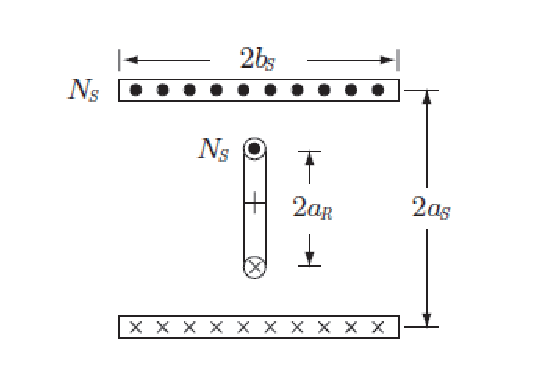
\includegraphics[scale=0.7]{chpt3/figs/fig3.15.eps}
	\caption{环形线圈置于薄壁线圈的中平面处}
\end{figure}

图3.15给出了两个线圈的安置示意图,图中环线圈位于薄壁螺管线圈的中平面上。在这个安置中,$\rho=-b_S$。这样,在方程3.98中插入$\rho=-b_S$,我们得到下面的简化表达式:
  \begin{equation}
  \begin{split}
M_{RS}(\rho=&-b_S)\simeq\frac{\mu_0}{2}(\frac{N_R N_S}{2b_S})\times\frac{2b_S}{\sqrt{(a_R+a_S)^2+b_S^2}}\times\\
&\{[(a_R+a_S)^2+b_S^2][K(\kappa)-E(\kappa)]-\Upsilon(c^2,k)\}%page113
\end{split}
\end{equation}

  式中,$k$为:
  \begin{equation}
\kappa^2=\frac{4a_Ra_S}{(4a_R+a_S)^2+b_S}%page113
\end{equation}

\textbf{特例4:长薄壁螺管和环线圈} 

当薄壁线圈是“长”的,特别是当$b_S\gg a_R$满足时,环线圈和螺管线圈的相对位置不再重要。对于一个满足$k^2\simeq 4a_R a_S/b_S^2$的长螺管,方程3.101变为:
\begin{equation}
\begin{split}
M_{RS}&\simeq\frac{\mu_0}{2}(\frac{N_RN_S}{2b_S})(2)\{b_S^2[K(\kappa)-E(\kappa)]-\Upsilon(c^2,\kappa)\}\\
&\simeq\frac{\mu_0}{2}(\frac{N_RN_S}{2b_S})\pi(a_R^2+a_S^2)[1-\frac{2(a_R-a_s)^2}{\pi(a_R^2+a_S^2)}\Pi(c^2,\kappa)]\\%page114
\end{split}
\end{equation}

大括号内的第二项可以视为修正项,在极限$ a_R\gg a_S$或$a_R\ll a_S$时可以忽略。

\textbf{特例5:与螺管直径相差很大的环线圈} 

当环线圈的直径与螺管线圈直径相差很大时,条件$c^2\rightarrow 0$满足,$\prod(c^2,0)$可由依$c^2$展开的级数的前几项表示。在方程3.102取极限$k^2\rightarrow 0(b_S\gg a_R,b_S\gg a_S),\prod(c^2,k)\rightarrow \prod(c^2,0)$时,使用3.49b,我们有:
  \begin{equation}
\begin{split}
M_{RS}&\simeq\frac{\mu_0}{2}(\frac{N_RN_S}{2b_S})\pi(a_R^2+a_S^2)[1-\frac{(a_R-a_s)^2}{(a_R^2+a_S^2)}(1+\frac{1}{2}c^2+\frac{3}{8}c^4+\frac{5}{16}c^6)]\\
&\simeq\frac{\mu_0}{2}(\frac{N_RN_S}{2b_S})\pi(a_R^2+a_S^2)\times \\
&\{1-\frac{(a_R-a_s)^2}{(a_R^2+a_S^2)}[1+\frac{2a_Ra_S}{(a_R^2+a_S^2)^2}+\frac{6(a_Ra_S)^2}{(a_R^2+a_S^2)^4}+\frac{20(a_Ra_S)^3}{(a_R^2+a_S^2)^6}]\}%page114
\end{split}
\end{equation}

\subsection{互感和相互作用力}
使用3.5.7节导出的轴向偏离中心线圈受到的轴向恢复力表达式,我们可以导出两个轴向依赖线圈的互感表达式。两个螺管A、B间的净磁力$F_{AB}$与存储在两个线圈中的总磁能有关:
\begin{equation}
\overrightarrow{F}_{AB}=\nabla E_{AB}%page114
\end{equation}

将方程3.92中的下标替换为方程3.104a中的A和B,注意到z向的$F_{AB}$是$F_{ZR}(\rho)$,我们有:
\begin{equation}
F_{zR}(\rho)=\frac{\partial E_{AB}}{\partial \rho}=I_AI_B\frac{\partial M_{AB}(\rho)}{\partial \rho}%pagr114
\end{equation}

对于小距离$\rho$($\rho\ll \sqrt{a_T^2+b_D^2}$),我们可以对$F_{ZR}(\rho)$积分,有:
\begin{equation}
M_{AB}(\rho)-M_{AB}(0)\propto-\rho^2%page114
\end{equation}

可见,对于小距离$\rho$,$M_{AB}(\rho)$随偏离中心距离的平方$\rho^2$减小。 


\textbf{磁场强度$H$和磁感应强度$B$}

除非特别指明,专题中的磁体都是空心的。此时,磁感应强度B和磁场强度H存在简单关系:$B=\mu_0 H$。式中,$\mu_0$是空气磁导率,此时等于真空磁导率。
通常,特别是工程师,常用特斯拉[T]作磁感应强度单位,用安培每米[A/m]作磁场强度的单位。

……cgs电磁单位制……

\newpage
\section{专题}
\subsection{讨论3.1:均匀电流密度螺管}

这里,我们首先讨论均匀电流密度螺管线圈的一些基本问题。绕组的内直径是$i.d.=2a_1$,外直径是$o.d.=2a_2$,总长度是$2b$。
图3.16定义了绕组截面——因为我们处理的是轴对称螺管,可以仅考虑z和r轴。由位于$(r,z)$处的微分截面载流环$dA \mathrm{[A/m^2]}$在中心点处产生的微分磁感性强度$dB_z(0, 0)$[T]为:
\begin{equation}
dB_z(0,0)=\frac{\mu_0r^2\lambda JdA}{2(r^2+z^2)^\frac{3}{2}}%page115
\end{equation}

式中,$\lambda J\mathrm{[A/m^2]}$是微分截面内部的总电流密度。无量纲数$\lambda$称为空间因子,这刻画了绕组截面并非完全由载流导体占据这一事实。注意到在这个模型中,$\lambda J$在整个绕组截面上是均匀的,且有:
\begin{equation}
\begin{split}
\lambda J&=\frac{NI}{2b(a_2-a_1)}\\
&=\frac{NI}{2a_1^2\beta(\alpha-1)}%page115
\end{split}
\end{equation}

式中,$\alpha=a_2/a_1,\beta=b/a_1$。$N$是总匝数,$NI$称为总安匝数。
\begin{figure}[htbp]
  \centering
 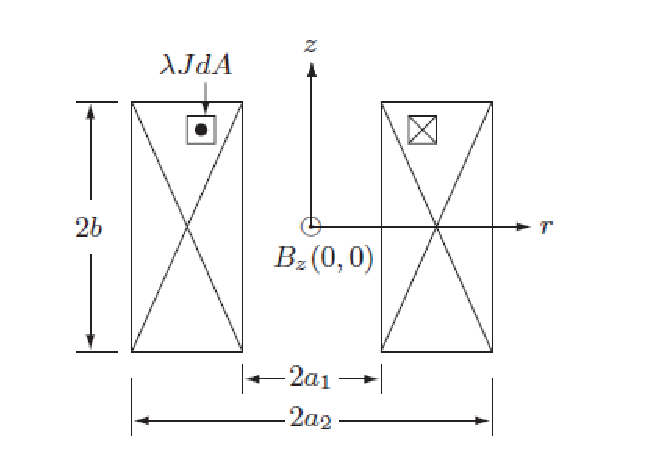
\includegraphics[scale=0.7]{chpt3/figs/fig3.16.eps}
  \caption{均匀电流密度螺管的截面}
\end{figure}

对3.107式从$r=a_1$到$r=a_2$以及$z=-b$到$z=b$积分,
我们得到螺管的$B_z(0,0)$和$F(\alpha,\beta)$的表达式:
\begin{eqnarray}
B_z(0,0)=\mu_0\lambda J_{a_1}F(\alpha,\beta)\\ %page116
F(\alpha,\beta)=\beta \ln\left(\frac{\alpha+\sqrt{\alpha^2+\beta^2}}{1+\sqrt{1+\beta^2}}\right)
\end{eqnarray}

前面已经提及,$F(\alpha,\beta)$是均匀电流密度线圈的“场因子”。和电感参数$L(\alpha,\beta)$类似,它也是仅依赖于螺管线圈的截面形状的。图3.17给出了三组关系:3.17a给出的是在$\beta$为常数时,$F(\alpha,\beta)$与$\alpha$的关系;3.17b给出的是在$\alpha$为常数时,$F(\alpha,\beta)$与$\beta$的关系;3.17a给出的是在$F(\alpha,\beta)$为常数时,$\beta$与$\alpha$的关系。

与$F(\alpha,\beta)$类似,螺管总体积$V_{cd}=\lambda 2\pi a_1^3(\alpha^2-1)\beta$在给定的$\lambda,a_1$条件下仅依赖于$\alpha,\beta$:每一幅图中的实线上的点都是给定$F(\alpha,\beta)$下的最小体积。$F(\alpha,\beta)$与某些特殊线圈相关的显著特征将在问题3.1中论及。

%%% 3个图自动编号????
%\begin{figure}
%  \centering
% 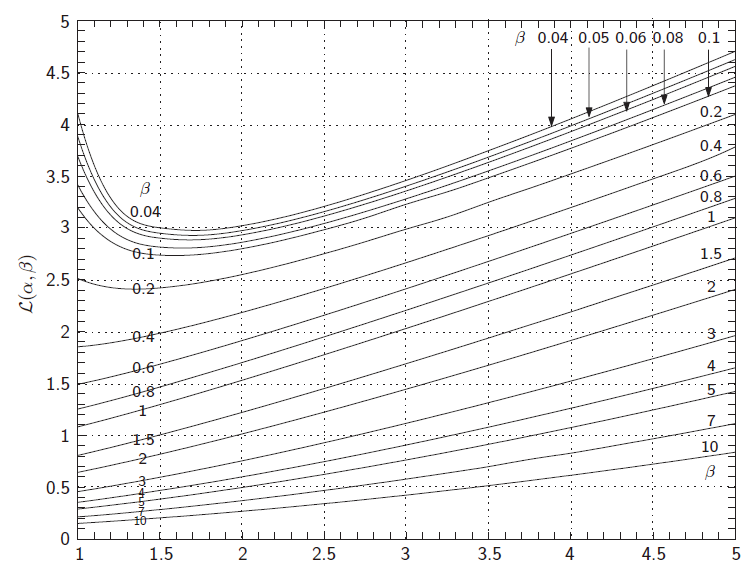
\includegraphics[scale=0.7]{figures/fig.3.14.png}
%  \caption{参数$\alpha,\beta$下的$\mathcal{L}(\alpha,\beta)$}
%\end{figure}
\begin{figure}
	\centering
	\subfigure[在$\beta$为常数时,$F(\alpha,\beta)$与$\alpha$的关系(虚线)。实线表示给定$F(\alpha,\beta)$下的最小导体体积。]
	{
		\label{fig:subfig:a} %% label for first subfigure
		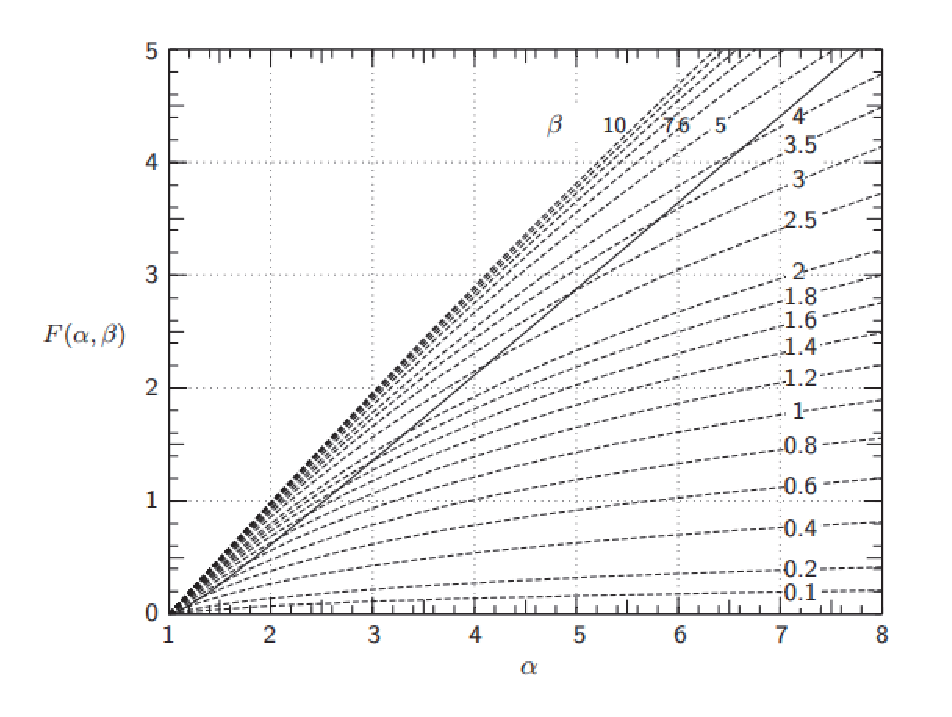
\includegraphics[scale=0.5]{chpt3/figs/fig3.17a.eps}}

	\subfigure[在$\alpha$为常数时,$F(\alpha,\beta)$与$\beta$的关系(虚线)。实线表示给定$F(\alpha,\beta)$下的最小导体体积。]
	{
		\label{fig:subfig:b} %% label for second subfigure
		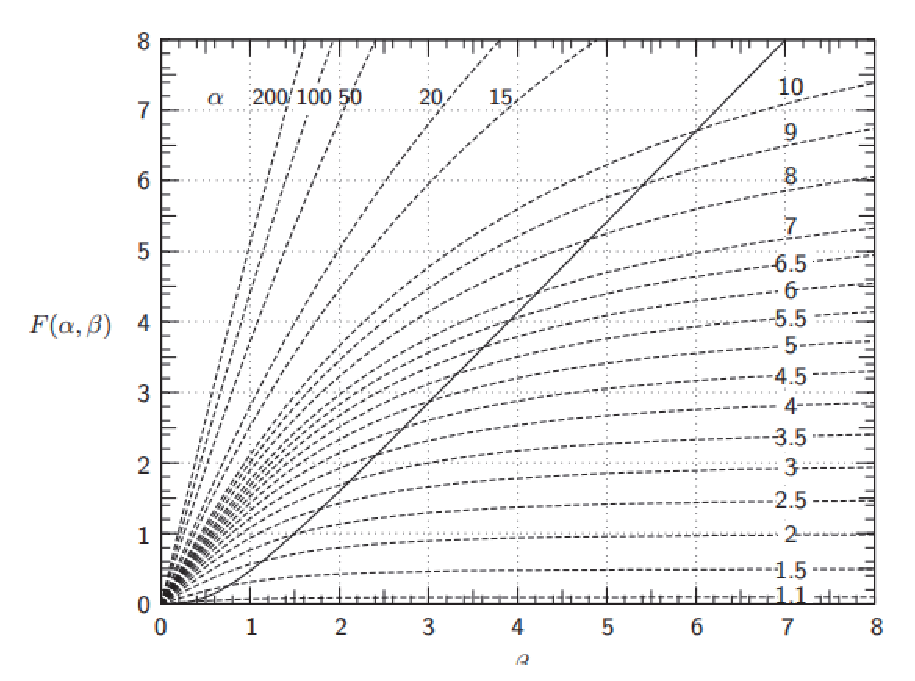
\includegraphics[scale=0.5]{chpt3/figs/fig3.17b.eps}}
	\subfigure[在$F(\alpha,\beta)$为常数时,$\beta$与$\alpha$的关系(虚线)。实线表示给定$F(\alpha,\beta)$下的最小导体体积。]
	{
		\label{fig:subfig:c} %% label for second subfigure
		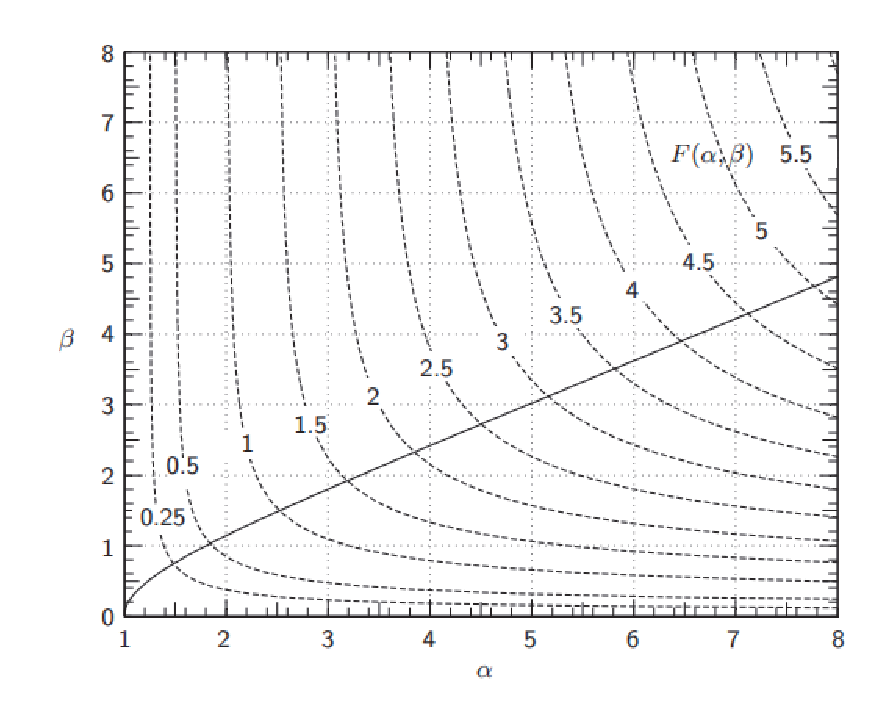
\includegraphics[scale=0.5]{chpt3/figs/fig3.17c.eps}}
	
	\caption{$F(\alpha,\beta)$、$\beta$、$\alpha$之关系}
	\label{fig:subfig} %% label for entire figure
\end{figure}

\subsection{问题3.1:“简单”螺管}
a)从3.107开始,推导得到3.109和3.13b。

b)通过联立3.108b和3.109,可以得到$B_z(0,0)$:
\begin{equation}
B_z(0,0)=\frac{\mu_0NI}{2a_1(\alpha-1)}\ln\left(\frac{\alpha+\sqrt{\alpha^2+\beta^2}}{1+\sqrt{1+\beta^2}}\right)\\%page118
\end{equation}
\begin{description}
  \item[“环”线圈] 化简上式为一个半径$a_1$、载流$NI$的环线圈($\alpha=1$),得到:
  \begin{equation}
    B_z(0,0)=\frac{\mu_0NI}{2a_1}%page118
  \end{equation}
 \item[“薄壁”螺管] 对于薄壁螺管($\alpha \rightarrow 1$),可以简化为:
 \begin{eqnarray}
   B_z(0,0)&=&\frac{\mu_0NI}{2a_1}\left(\frac{1}{\sqrt{1+\beta^2}}\right)\\ %page118
   B_z(0,0)&=&\mu_0 \lambda Ja_1(\alpha-1)\frac{\beta}{\sqrt{1+\beta^2}}%page118
 \end{eqnarray}
  \item[“长”螺管] 对于长度远大于外直径的螺管($\beta \gg \alpha$),可以简化为:
\begin{equation}
B_z(0,0)=\frac{\mu_0NI}{2b}%page118
\end{equation}
考虑到$NI/2b=K_\theta$,上式等价于3.5,于是
\begin{equation}
B_z(0,0)=\mu_0\lambda Ja_1(\alpha-1)%page118
\end{equation}
  \item[“饼式”线圈] 对于长度比外直径小很多的饼式线圈,简化为:
  \begin{equation}1
B_z(0,0)=\frac{\mu_0NI}{2a_1}(\frac{\ln\alpha}{\alpha-1})%page118
  \end{equation}
\end{description}

c)\textbf{场 vs. 能量}:证明电阻性螺管(比如铜螺管)线圈的中心场表达$B_z(0,0)$与其所需功率$P$的关系为:
\begin{eqnarray}
B_z(0,0)&=&\mu_0G(\alpha,\beta)\sqrt{\frac{\lambda P}{\rho_{cd}a_1}}\\ %page118
G(\alpha,\beta)&=&\sqrt{\frac{\beta}{2\pi(\alpha^2-1)}}\ln(\frac{\alpha+\sqrt{\alpha^2+\beta^2}}{1+\sqrt{1+\beta^2}})%page118
\end{eqnarray}
式中,$\rho_{cd}$是导体电导率。$G(\alpha,\beta)$被称为均匀电流密度线圈的“G因子”。

\subsubsection{问题3.1之解}

a)对3.107在$z$和$r$的合适区间积分,得到:
\begin{equation}
B_z(0,0)=\frac{\mu_0\lambda J}{2}\int_{a_1}^{a_2}\int_{-b}^{b}\frac{r^2dzdr}{\sqrt[3]{r^2+z^2}}=\mu_0\lambda J\int_{a_1}^{a_2}\int_{0}^{b}\frac{r^2dzdr}{\sqrt[3]{r^2+z^2}}%page119
\end{equation}

查积分表,得到:
\begin{equation}
\int_{0}^{b}\frac{dz}{\sqrt[3]{r^2+z^2}}=\left[\frac{z}{r^2\sqrt{r^2+z^2}}\right]_{0}^{b}=\frac{b}{r^2\sqrt{r^2+b^2}}%page119
\end{equation}

于是:
\begin{equation}
\begin{split}
B_z(0,0)&=\mu_0\lambda J\int_{a_1}^{a_2}\frac{r^2bdr}{r^2\sqrt{r^2+b^2}}=\mu_0\lambda Jb[\ln({r+\sqrt{r^2+b^2}})]_{a_1}^{a_2}\\
&=\mu_0\lambda Jb[\ln(a_2+\sqrt{a_2^2+b^2})-\ln(a_1+\sqrt{a_1^2+b^2})]\\
&=\mu_0\lambda Ja_1\left(\frac{b}{a_1}\right)\ln\left[\frac{\frac{a_2}{a_1}+\sqrt{(\frac{a_2}{a_1})^2+(\frac{b}{a_1})^2}}{(\frac{a_1}{a_2})+\sqrt{(\frac{a_1}{a_1})^2+(\frac{b}{a_1})^2}}\right]\\%page119
\end{split}
\end{equation}

考虑到$a_2/a_1=\alpha$和$b/a_1=\beta$,上式变为:
\begin{equation}
B_z(0,0)=\mu_0\lambda J\alpha_1\beta\ln\left[\frac{\alpha+\sqrt{\alpha^2+\beta^2}}{1+\sqrt{1+\beta^2}}\right]%page119
\end{equation}

于是:
\begin{eqnarray}
% \nonumber % Remove numbering (before each equation)
B_z(0,0)&=&\mu_0\lambda J_{a_1}F(\alpha,\beta)\\ %page119
F(\alpha,\beta)&=&\beta \ln\left(\frac{\alpha+\sqrt{\alpha^2+\beta^2}}{1+\sqrt{1+\beta^2}}\right)%page119
\end{eqnarray}

b)\textbf{“环”线圈}。对于环线圈($\alpha\rightarrow 1; \beta\rightarrow 0$),3.110中右侧的对数项成为:
\begin{equation}
\lim_{\beta\rightarrow 0}\ln\frac{\alpha+\sqrt{\alpha^2+\beta^2}}{1+\sqrt{1+\beta^2}}=\ln\alpha%page119
\end{equation}

因为当$|\epsilon|\ll 1$时,$\ln (1+\epsilon)\simeq \epsilon$。故有$\alpha\rightarrow 1$时,$\ln \alpha\rightarrow \alpha-1$。于是:
\begin{equation}
B_z(0,0)=\frac{\mu_0NI}{2a_1(\alpha-1)}(\alpha-1)=\frac{\mu_0NI}{2a_1}%page119
\end{equation}
注意到,方程3.111a和方程3.3a的关系。

\textbf{薄壁螺管。}对于薄壁螺管($\alpha\rightarrow 1$),通过联立3.13b和3.23b,可得:
\begin{equation}
\lim_{\alpha\rightarrow 1}\ln\frac{\alpha+\sqrt{\alpha^2+\beta^2}}{1+\sqrt{1+\beta^2}}=\frac{\alpha-1}{\sqrt{1+\beta^2}}%page120
\end{equation}

联立3.110和S1.3,我们得到3.111b。从方程3.109,3.13b和S1.3,我们得到3.111c:
\begin{eqnarray}
B_z(0,0)&=&\frac{\mu_0 NI}{2a_1}(\frac{1}{1+\beta^2})\\ %page120
B_z(0,0)&=&\mu_0 \lambda Ja_1(\alpha-1)\frac{\beta}{\sqrt{1+\beta^2}}%page120
\end{eqnarray}

注意到,对于长螺管$\beta\gg 1$,3.111c变成3.111e。

\textbf{长螺管。}对于$\beta\gg \alpha$,有:
\begin{equation}
\lim_{\beta\gg\alpha}\ln\left(\frac{\alpha+\sqrt{\alpha^2+\beta^2}}{1+\sqrt{1+\beta^2}}\right)=\ln\left(\frac{\alpha+\beta}{1+\beta}\right)=\ln\left(\frac{\frac{\alpha}{\beta}+1}{\frac{1}{\beta}+1}\right)%page120
\end{equation}

使用“环”线圈中相同的近似方法,得到:
\begin{equation}
\lim_{\beta\gg\alpha}\ln\left(\frac{\frac{\alpha}{\beta}+1}{\frac{1}{\beta}+1}\right)\simeq\frac{\alpha}{\beta}-\frac{1}{\beta}=\frac{\alpha-1}{\beta}%page120
\end{equation}

于是在极限$\beta\gg\alpha$下,我们得到:
\begin{equation}
B_z(0,0)=\frac{\mu_0NI}{2b}%page120
\end{equation}

上文已经提及,$NI/2b$可以视为表面电流密度。从式3.108中,有$NI/(2b)=\lambda J (a_2-a_1)$。于是上式又可以写为:
\begin{equation}
B_z(0,0)=\mu_0\lambda Ja_1(\alpha-1)%page120
\end{equation}

对于一个长螺管,它的中心场和它的长度是无关的。$B_z(0,0)$独立性在大$\beta(>\sim 3)$和中等$\alpha(<\beta)$情况下是明显的(图3.17b)。
同样,$B_z(0,0)$在大$\beta(>\sim 3)$和中等$\alpha(<\beta)$情况下正比于线圈的$a_2-a_1$。这是因为该值越大,对应的单位长度总安匝数越大(图3.17a)。

\textbf{饼式线圈。}对于饼式线圈,近似极限是$\beta\rightarrow 0$:
\begin{eqnarray}
\lim_{\beta\rightarrow 0}\ln\frac{\alpha+\sqrt{\alpha^2+\beta^2}}{1+\sqrt{1+\beta^2}}=\ln\left(\frac{2\alpha}{2}\right)=\ln\alpha\\%page120
B_z(0,0)=\frac{\mu_0NI}{2a_1}\left(\frac{\ln\alpha}{\alpha-1}\right)%page120
\end{eqnarray}

注意到,饼式线圈的中心场等于环线圈的中心场乘一个系数$\ln \alpha/(\alpha-1)$。在$\alpha\rightarrow 1$时,上式退化为环线圈的表达式。

c)全部导体体积等于$\lambda\times$<绕组体积(winding volume, wv)>:
\begin{equation}
<wv>=2b\pi(a_2^2-a_1^2)=a_1^32\pi\beta(\alpha^2-1)%page121
\end{equation}

于是:
\begin{equation}
P=\rho_{cd}J^2\lambda a_1^32\pi\beta(\alpha^2-1)%page121
\end{equation}

这里,$J$仅是导体中的电流密度。从3.112中,我们用$P$和其他参数解出$J$:
\begin{equation}
J=\sqrt{\frac{P}{\rho_{cd}\lambda a_1}}\left[\frac{1}{a_1\sqrt{2\pi\beta(\alpha^2-1)}}\right]%page121
\end{equation}

联立S1.2和S1.4,得到:
\begin{equation}
\begin{split}
B_z(0,0)&=\mu_0\lambda\sqrt{\frac{P}{\rho_{cd}\lambda a_1}}\left[\frac{1}{a_1\sqrt{2\pi\beta(\alpha^2-1)}}\right]a_1\beta\ln(\frac{\alpha+\sqrt{\alpha^2+\beta^2}}{1+\sqrt{1+\beta^2}})\\
&=\mu_0\sqrt{\frac{\lambda P}{\rho_{cd}a_1}}\sqrt{\frac{\beta}{2\pi(\alpha^2-1)}}\ln\left(\frac{\alpha+\sqrt{\alpha^2+\beta^2}}{1+\sqrt{1+\beta^2}}\right)%page121
\end{split}
\end{equation}

于是:
\begin{eqnarray}
B_z(0,0)&=&\mu_0G(\alpha,\beta)\sqrt{\frac{\lambda P}{\rho_{cd}a_1}}\\ %page121
G(\alpha,\beta)&=&\sqrt{\frac{\beta}{2\pi(\alpha^2-1)}}\ln\left(\frac{\alpha+\sqrt{\alpha^2+\beta^2}}{1+\sqrt{1+\beta^2}}\right)%page121
\end{eqnarray}

上式表明,对给定参数$\alpha$和$\beta$的电阻性螺管线圈所需的功率P和它的中心场是平方关系:
\begin{equation}
P=\frac{\rho_{cu}a_1B_z^2(0,0)}{\mu_0^2\lambda G^2(\alpha,\beta)}%page121
\end{equation}

\newpage
\subsection{讨论3.2:Bitter磁体}
尽管本书主要研究超导磁体,这里我们讨论一下无铁芯、水冷磁体。我们称这种直流高场水冷磁体为“Bitter磁体”,以纪念于1930s最早提出该设计的MIT科学家Francis Bitter。
Bitter的工作奠定了现代磁体技术的基础。
我们从Bitter的《磁体》一书摘录一段,描述高场磁体的技术挑战和解决方案。


Bitter的设计采用了堆叠的环形板导体。每一个板有一个缝,用薄绝缘片隔开。缝允许裸露部分在压力下与相邻板的裸露部分连接,从而电流可以在板间以类似螺旋的形式流动。
每一个Bitter板都打了数百个冷却孔。为了产生高场,通入几千安培的电流,小号几兆瓦的电能,转换为金属板的热量。迫流水以高速($\sim 20\ \mathrm{m/s}$)流过孔,带走热量。
1990s国家高场实验室开发的Florida-Bitter磁体如图3.18所示。板上的径向缝清晰可见。同时也注意到,水控并不是像Bitter板是圆形的。这种在电流方向拉长的形状处理最早是由
MIT的Weggel在1970s提出的。这里的外板直径是$148\ \mathrm{mm}$;板直径尺寸早已超过$400\ \mathrm{mm}$。16个大孔是用于板的轴向固定的。Bitter磁体制造的关键特征是模块化,即由
许多相似的板组成。为了优化磁体性能,板的厚度、机械性质和电气性质在轴向可以定制。

由3.110式可知,在给定安匝数$NI$下,绕组内径$a_1$越小,中心场$B_z(0,0)$越大。又,从3.113a式可知,在相同功耗下,安匝越靠近磁体室温孔越高效。
Bitter的设计($J\propto 1/r$)是一个近似实现上述目标的有效方法。

%%%%图3.18 
\begin{figure}[htbp]
  \centering
 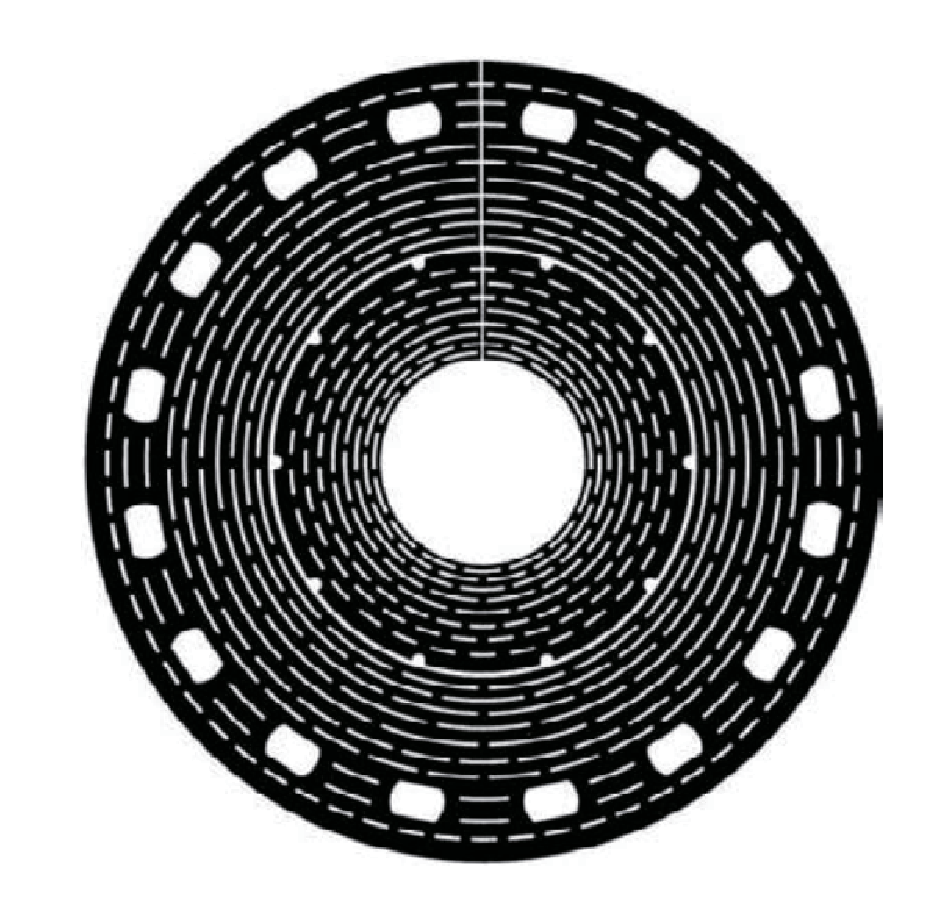
\includegraphics[scale=0.5]{chpt3/figs/fig3.18.eps}
  \caption{国家高场实验室的两个嵌入式Florida-Bitter轮廓,外盘直径140\ mm,位于“水”磁体内}
\end{figure}

\textbf{A. 电流密度、场、能量}

本节,我们推导出Bitter磁体的以下表达式:电流密度$J_\theta (r)$,中心场$B_z(0,0)$,场因数$F(\alpha,\beta)$,G因数$G(\alpha,\beta)$。

\textbf{电流密度分布}

考虑一个单盘,电流在$\theta$向流动。电场E给出的电压V正比于$\theta$。因为$\vec{E}$仅有$\theta$分量,且在给定r处为常亮,$E_\theta 2\pi r=V$。
所以,$E_\theta$按照$1/r$变化。由于$\vec{J}=\vec{E}/\rho_{Cu}$,我们有:
\begin{equation}
{[J_\theta(r)]}_B=\frac{E_{\theta}}{\rho_{cu}}=\frac{V}{2\pi\rho_{cu}r}=J_0\frac{a_1}{r}%page123
\end{equation}

式中,$J_0=[J_\theta(a_1)]_B=V/(2\pi \rho_{Cu} a_1)$。上式表明,Bitter磁体中的电流密度按照$1/r$减小,且在$r=a_1$处取得最大值。

\textbf{场}

我们用上式给出的$J_\theta$替换3.107式中的$\lambda J$。选择合适的上下限,积分得:
\begin{equation}
\begin{split}
{[B_z(0,0)]}_B&=\mu_0\lambda_B J_0a_1\int_{a_1}^{a_2}\int_{0}^{b}\frac{r dr dz}{\sqrt[3]{r^2+z^2}}\\
&=\mu_0\lambda_B J_0 a_1\int_{1}^{\alpha}\int_{0}^{\beta}\frac{\eta d\eta d\zeta}{\sqrt[3]{\eta^2+\zeta^2}}%page123
\end{split}
\end{equation}

式中,$r/a_1=\eta$,$z/a_1=\zeta$,查积分表,得到:
\begin{equation}
\int_{0}^{\beta}\frac{d\zeta}{\sqrt[3]{\eta^2+\zeta^2}}=\left[\frac{\zeta}{\eta^2\sqrt{\eta^2+\zeta^2}}\right]_0^{\beta}=\frac{\beta}{\eta^2\sqrt{\eta^2+\beta^2}}%page123
\end{equation}

联立上面两式,得到:
\begin{equation}
\begin{split}
{[B_z(0,0)]}_B&=\mu_0\lambda_B J_0a_1\beta\int_{1}^{\alpha}\frac{\eta d\eta}{\eta^2\sqrt{\eta^2+\beta^2}}\\
&=\mu_0\lambda_B J_0a_1\beta\left[-\frac{1}{\beta}\ln(\frac{\beta+\sqrt{\beta^2+\eta^2}}{\eta})\right]_1^{\alpha}\\ %page123
&=\mu_0\lambda_B J_0a_1\ln\left(\alpha\frac{\beta+\sqrt{1+\beta^2}}{\beta+\sqrt{\alpha^2+\beta^2}}\right)%page123
\end{split}
\end{equation}

上面的表达式可以写为:
\begin{eqnarray}
% \nonumber % Remove numbering (before each equation)
{[B_z(0,0)]}_B&=&\mu_0\lambda_B J_0a_1[F(\alpha,\beta)]_B\\ %page123
{[F(\alpha,\beta)]}_B&=&\ln\left(\alpha\frac{\beta+\sqrt{1+\beta^2}}{\beta+\sqrt{\alpha^2+\beta^2}}\right)%page123
\end{eqnarray}

注意3.115b和3.15b两式的区别。

\textbf{场和能量}

我们通过在整个线圈区域内积分功率密度$\rho_{Cu} [J_\theta]_B^2(r)$推导出$[H_z(0,0)]_B$和Bitter磁体总功率$P_B$的关系式。这里继续采用无量纲参数,有:
\begin{equation}
P_B=a_1^3\int_{1}^{\alpha}\int_{-\beta}^{\beta}\rho_{cu}\lambda_B\left(\frac{J_0}{\eta}\right)^2 2\pi\eta d\zeta d\eta=J_0^2\rho_{cu}\lambda_B a_1^3(4\pi\beta\ln\alpha)%page124
\end{equation}

通过上面的表达式,我们将$J_0$和$P_B$联系起来:
\begin{equation}
J_0=\frac{1}{a_1\sqrt{4\pi\beta\ln\alpha}}\sqrt{\frac{P_B}{\rho_{cu}\lambda_B a_1}}%page124
\end{equation}

上式和3.115联立,得到:
\begin{equation}
{[B_z(0,0)]}_B=\mu_0[G(\alpha,\beta)]_B\sqrt{\frac{\lambda_B P_B}{\rho_{cu}a_1}}%page124
\end{equation}

式中,
\begin{equation}
{[G(\alpha,\beta)]}_B=\frac{1}{\sqrt{4\pi\beta\ln\alpha}}[F(\alpha,\beta)]_B%page124
\end{equation}

在均匀电流密度螺管线圈中,$[B_z(0,0)]_B$按$P_B$的平方根增加;$P_B$是磁场的二次函数。
$[G(\alpha,\beta)]_B$在$\alpha\simeq 6.42$和$\beta\simeq 2.5$时取得最大值,此时$[G(\alpha,\beta)]_B\simeq 0.166$。在$5\leq \alpha \leq 9$和$1.8\leq\beta\leq 2.6$范围内,$[G(\alpha,\beta)]_B$的值
至少是其峰值的99\%。也就是说,在这个$\alpha$和$\beta$范围内,在给定场下,$P_B$变动在2\%以内。
不过,给定$a_1$时,场的均匀性随$2b/\beta$增大而改善。故大多数Bitter磁体的$\beta>2.5$。

\textbf{实例}

我们用上面的关系式计算一个Bitter磁体。磁体参数$2a_1=6\ \mathrm{cm}, 2a_2=40\ \mathrm{cm}, 2b=22 \ \mathrm{cm},\lambda_B=0.8, \rho_{Cu}=2\times10^{-6}\ \mathrm{\Omega cm}$,产生的磁场$[B_z(0,0)]_B=20\ \mathrm{T}$。
此时,$\alpha=40/6=6.67;\beta=22/6=3.67$。
\begin{equation}
\begin{split}
{[G(6.67,3.67)]}_B&=\frac{1}{\sqrt{4\pi3.67\ln(6.67)}}\ln\left[6.67\frac{3.67+\sqrt{1+(3.67)^2}}{3.67+\sqrt{(6,67)^2+(3.67)^2}}\right]\\
&\simeq 0.159 %page124
\end{split}
\end{equation}

类似的,
\begin{equation}
\begin{split}
P_B&=\frac{\rho_{cu}a_1[B_z(0.0)]_B^2}{\mu_0^2\lambda_B[G(\alpha,\beta)]_B^2}\\
&=\frac{(2\times 10^{-8}\ \Omega m)(3\times 10^{-2}\ \mathrm{m})(20\ \mathrm{T})^2}{(4\pi\times 10^{-7}\ \mathrm{\frac{H}{m}})^2(0.8)(0.159)^2}\\
&\simeq 7.5\ \mathrm{MW}%page124
\end{split}
\end{equation}

这个功率是运行于Francis Bitter国家磁体实验室$20\ \mathrm{T}$ Bitter磁体的典型值。

\textbf{B. 非“Bitter”电流密度分布}

水冷磁体的一个重要参数是磁场效率,定义为$[B_z(0,0)]_B^2/\mu_0^2 P_B$。作为一种均匀电流密度磁体,Bitter磁体的场效率正比于$\lambda_B$和$[G(\alpha,\beta)]_B^2$,反比于
$a_1$和$\rho_{Cu}$。

我们到目前讨论了两种电流分布:1)均匀电流分布,$J(r,z)=J_0$。这时,J与r和z无关;2)Bitter分布,即$J\propto 1/r$。
由graded超导材料绕的超导磁体的$J(r)$随r离散阶梯变化。由多个嵌套线圈组成的磁体,每一个线圈由不同的超导带绕成,同样有$J(r)$随r阶梯变化。此处,我们介绍另外三种水冷磁体的电流分布。

\textbf{Kelvin线圈}

给出最高磁场效率的电流密度分布被称为Kelvin分布:
\begin{equation}
J_K(r,z)\propto\frac{r}{(r^2+z^2)^\frac{3}{2}}%page125
\end{equation}

Kelvin线圈的独有性质是每一个部分的单位功率都产生相同的磁场。
作为对比,总功率相同的均匀电流密度线圈的中心场仅为Kelvin线圈的66\%;Bitter线圈的这个比值是77\%。不过,制成具有Kelvin电流分布的线圈并不具可行性。

\textbf{Gaume}

Gaume分布同样给出很好的磁场效率:
\begin{equation}
J_G(r,z)\propto\frac{1}{r}\left(\frac{1}{\sqrt{a_1^2+z^2}}-\frac{1}{\sqrt{a_2^2+z^2}}\right)%page125
\end{equation}

Gaume线圈的每一匝在单位功率下产生相同的磁场。Gaume线圈的磁场是Kelvin的85\%。Bitter线圈的电流分布在某种程度上是近似于Gaume线圈的。这可以通过以下方法实现:
更厚的Bitter板,轴向远离中心平面。$J_b(r,z)\propto 1/r\delta(z)$,此处$\delta(z)$是依赖于z的板的厚度。

\textbf{Polyhelix}

多螺旋线圈由多个嵌套的单层线圈组成,每一层的电流密度被调整以最大化磁场效率和/或匹配每一层的与其导体强度匹配的应力:
\begin{equation}
J_P(r,z)\propto f(r)%page125
\end{equation}

最高效率的多螺旋线圈,其$J_P(r,z)\propto 1/r^2$,可以产生92\%的Kelvin磁场。实践中,由于两端需要多个电极,多螺旋线圈被认为比Bitter线圈更难于制造。
\newpage


\subsection{问题3.2:螺管中的最大场}
虽然磁体中心的轴向场是磁体用户通常要确认的参数,但对磁体设计者来说同等重要的一个参数
是磁体暴露的最大场。在但螺管磁体中,如方程3.12b给出的,中平面轴向场$H_z(r,
\theta)$在室温孔内随远离轴而快速增长。
实际上,轴向的最大场出现在中平面的绕组半径最内点:$H_m=H_z(a_1,0)$。
在由多个嵌套线圈组成的多线圈磁体中,最大场反而不再最内线圈上。这是由于其余线圈产生的场
通常并非轴向,是偏移$(a_1,0)$点的。
再次说明,对这个话题的处理只是为了增强读者对简单螺管线圈场分布的理解。在实际的多线圈磁体中,
必须依靠程序代码来计算最大场及其所处的位置。

a)使用3.4节中的表达式,证明对“薄壁”线圈($\alpha=1$),有关系式$H_z(r,0)/H_z(0,0)=h_z(\xi)$,其中$\xi=r/a_1$:
\begin{equation}
\begin{split}
h_z(\xi)&=1+\frac{3}{4(1+\beta^2)^2}\xi^2+\frac{15(3-4\beta^2)}{64(1+\beta^2)^4}\xi^4+\frac{35(5-20\beta^2+8\beta^4)}{256(1+\beta^2)^6}\xi^6\\
&+\frac{315(35-280\beta^2+336\beta^4-64\beta^6)}{16384(1+\beta^2)^8}\xi^8\\
&+\frac{693(63-840\beta^2+2016\beta^4-1152\beta^6+128\beta^8)}{65536(1+\beta^2)^{10}}\xi^{10}%page126
\end{split}
\end{equation}

b)此外,证明对“短”线圈($\beta=0$),$h_z(\xi)$的表达式为:
\begin{equation}
\begin{split}
h_z(\xi)&=1+\frac{3(\alpha^2-1)}{8\alpha^2\ln\alpha^2}\xi^2+\frac{45(\alpha^4-1)}{256\alpha^4\ln\alpha}\xi^4+\frac{175(\alpha^6-1)}{1536\alpha^6\ln\alpha}\xi^6\\
&+\frac{11025(\alpha^8-1)}{131027\alpha^8\ln\alpha}\xi^8+\frac{43659(\alpha^10-1)}{655360\alpha\ln\alpha}\xi^{10}\cdots%page126
\end{split}
\end{equation}

c)类似的,证明对“薄壁且长”线圈,$h_z(\xi)$为:
\begin{equation}
h_z(\xi)\propto1+\frac{3}{4\beta^4}\xi^2-\frac{15}{16\beta^6}\xi^4+\frac{35}{32\beta^8}\xi^6-\frac{315}{256\beta^{10}}\xi^8+\cdots%page126
\end{equation}

d)对“薄壁”线圈($\alpha=1$)和相对“短”线圈($\beta=0.4$)计算$H_m/H_z(0, 0)\equiv h_m$的近似值。

e)计算饼式线圈($\alpha=2,\beta\simeq 0$)的$h_m$。

f)确定“薄壁”且“长”线圈($\alpha=1,\beta=2$)的$h_m$。 

\subsubsection{问题3.2之解}
a) 考虑到$H_z(r,\theta)$在中平面上与$H_z(x, 0)$或$H_z(y, 0)$等价,我们使用方程3.12b,其中$\xi = x/a_1$,$\xi = y/a_1$或$\xi = r/a_1$。对于“薄壁”螺管线圈,我们可以通过联立方程3.12b和3.25得到方程3.117a。

b) 类似的,方程3.117b可以通过联立方程3.12b和3.21得到。

c) 我们通过联立3.12b和3.26得到方程3.117c。不像方程3.117b的高阶项的符号都是正的,
3.117c中的项是正负交替的。 

d) 将$\beta=0.4,\xi=1$代入方程3.117a,我们得到:
$$h_m=1 + 0.5574 + 0.3055 + 0.1125 − 0.0086 − 0.0585 = 1.9082$$

e) 将$\alpha=2,\xi=1$代入方程3.117b,我们得到:
$$ h_m=1 + 0.4058 + 0.2378 + 0.1618 + 0.1209 + 0.0960 = 2.0222$$

f) 将$\beta=2,\xi=1$代入方程3.117a,我们得到:
$$ h_m=1 + 0.03 − 0.0049 + 0.0005 + 0.0000 − 0.0000 = 1.0256 $$

一个更快但稍不精确的解可以从方程3.117c中得到,该方程事实上只对$\beta\gg 1$成立:
$$h_m \simeq 1 + 0.0469 − 0.0146 + 0.0043 − 0.0012 + 0.0003 = 1.0356$$

\newpage

\subsection{讨论3.3:负荷线}
\textbf{A. 用“各向同性”超导体绕成的螺管线圈磁体}

图3.19给出了各向同性超导体在给定温度$T_0$下临界电流$I_c$与$B$的关系曲以及超导螺管磁体的两组“负荷线”。
这里,$I_c(B,T_0)$是各向同性的,也即$I_c(B,T_0)$与场方向无关,这和圆截面超导体的特性是吻合的。

实线和虚线负荷线,从对应“自场”的$B_z(0,0)$开始:实线对应轴向场$B_z(0,0)$,虚线代表绕组内的最大场$B_{mx}$——对简单螺管磁体,$B_{mx}$出线在绕组内半径($r=a_1$)和轴向中平面($z=0$)处,$B_{mx}=B_z(a_1,0)$。
$I_c(B,T_0)$和虚线负载线交点是磁体可以保持超导态的可获得最大运行电流,$I_{op}(B_{mx},T_0)$。

当磁体置于另一个磁体的室温孔中,背景场磁体产生的场必将加到内侧磁体的负载线上,
所谓的“内插”——在一个组合系统中,两个磁体一般是同轴且中平面重合的。
从B轴上$B_{b}$开始的实线对应组合系统中心场,虚线对应最大内插场——注意到虚线起点略高于$B_{b}$,因为那里的背景场更大;$I_c(B,T_0)$和虚线的交点给出了这个组合磁体系统的最大运行电流,$I_{op}(B_{mxb},T_0)$。

出于各种原因,后面各章节讨论的超导磁体,不论是孤立的还是组合的系统,一般设计运行电流
为其最大可能电流的50–70\%。

\begin{figure}[htbp]
	\centering
	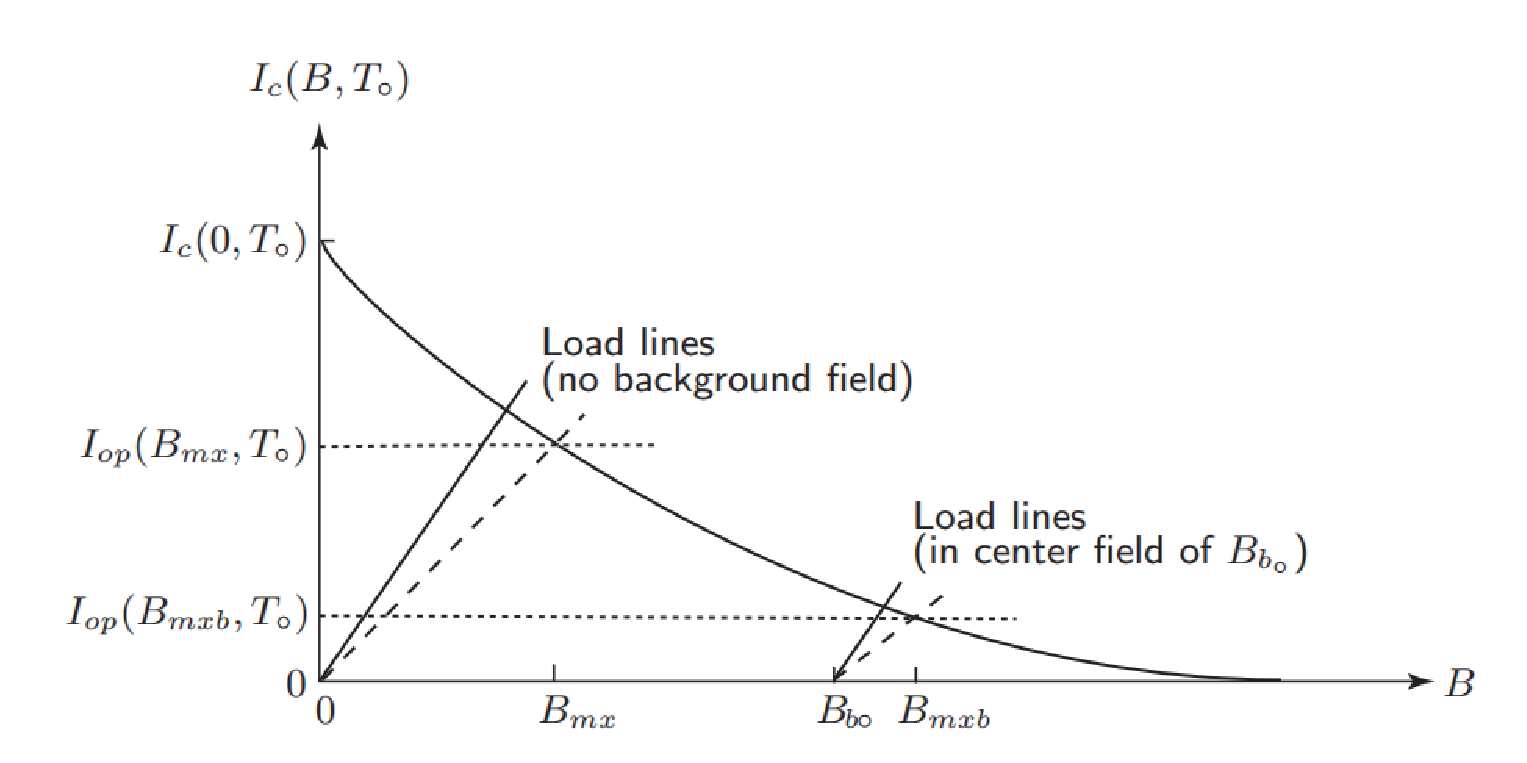
\includegraphics[scale=0.4]{chpt3/figs/fig3.19.eps}
	\caption{各向同性超导体在给定温度$T_0$下临界电流$I_c$与$B$的关系曲线;螺管磁体的两组“负荷线”——自场以及置于另一个产生背景中心场$B_{b0}$的螺管磁体室温孔中两种情况}
\end{figure}

\textbf{B. 用各向异性超导体绕制的螺管磁体}

对于一个非圆截面超导体,$I_c(B,T_0)$通常是“各向异性”的,即$I_c(B,T_0)$依赖于磁场相对于截面的方向。
非圆截面超导体的典型例子就是高温超导体Bi2223和YBCO,这两种导体都是“带”式的。

附录V中给出了Bi2223和YBCO的$I_c(B, T)/I_c(sf,77\ \mathrm{K})$图——$I_c(B, T)$数据归一化为$I_c(sf,77\ \mathrm{K})$数据。所谓sf,代表“自场”(self field),即传导电流自身产生的磁场。对每一种超导体,给出了两组数据,一组是外部施加平行垂直电流“宽”面的磁场$B_{\parallel}$,一组是外部施加垂直于“宽”面的磁场$B_{\perp}$。 
Bi2223和YBCO的$I_c(B,T_0)$都是在$B_{\perp}$下下降更快。
另一个值得注意的是,两种导体的临界电流在两种方向的磁场下,都是磁场越大下降越快。

可以从图3.3所示的螺管磁体的场线可以推断出,径向分量$B_r$在螺管轴向中平面($z=0$)严格为零,
在$\pm b$和$r$方向增长,在$z=\pm b,a_1 < r < a_2$存在最大径向场$[B_r(\alpha,\beta)]_{pk}$。
不存在$[B_r(\alpha,\beta)]_{pk}$的闭式解析解。
不过,对于大多数但螺管线圈($1\le \alpha \le 3.6 , 0.1\le \beta \le 10$),在基于带材的磁体初设阶段,例如双饼线圈堆叠磁体(讨论3.6),方程3.118给出的$[B_{r}(\alpha,\beta)]_{pk}$与程序代码计算的结果相差$\pm 30\%$:
\begin{equation}
 \frac{[B_{r}(\alpha,\beta)]_{pk}}{B_{z}(0,0)}\simeq\frac{0.3}{\alpha^{2}\beta}+\frac{0.6}{\alpha}\\%(3.118)
\end{equation}

注意到,对一个“薄壁”或“中等厚壁” ($\alpha \le 1.8$) 且“短” ($\beta < 1$) 的螺管线圈,
$[B_r(\alpha,\beta)]_{pk}$ 可能超过$B_z(0, 0)$,例如$[B_r(\alpha=1.1,\beta=0.1)]_{pk}\approx 3B_z(0,0)$!

从而,由带材绕制的磁体中,负荷线交点对应最大垂直场$B_{\perp}$,即$[B_r(\alpha,\beta)]_{pk}$。
限制带材运行电流的是带材的$I_c(B_{\perp},T_0)$曲线而不是对应$I_c(B, T_0)$的最大$B(=B_z)$负荷线。
同时,由于$B_{\perp}$随绕组中带材的高度(带材宽度)而变化,
这个变化在计算最大运行电流的时候也必须包括进来。
Voccio最近给出了确定Bi2223和YBCO带材绕制的“饼式线圈”的最大运行电流的解析方法[3.10]。

\newpage

\subsection{讨论3.4:叠加技术}
解场问题应用的Biot-Savart定律从根本上阐明了螺管上某点的磁场是螺管上所有电流源产生的磁场的矢量和叠加。
这里,我们在整个螺管上应用叠加技术以计算螺管轴线上任一点的磁场。这个技术,虽仅限于轴线上的磁场,但亦能
增进读者对螺管磁场的一般理解。

\textbf{A. 末端磁场}

轴对称螺管的轴线末端处磁场是一个同样组成但两倍长度的螺管的中心场的一半。
我们可以形象化的理解这个问题,考虑一个有两个完全相同部分组成的轴对称螺管,每个螺管长$2b$(图3.20)。
新螺管的轴向中心场是由两个部分螺管产生的两个等量场之和:
\begin{equation}
H(b)=H(\alpha,\beta)|_{z=b}=\frac{1}{2}H(\alpha,2\beta)|_{z=0}=\frac{1}{2}\lambda Ja_{1}[F(\alpha,2\beta)]\\%(3.119)
\end{equation}

由于$F(\alpha, 2\beta)>F(\alpha,\beta)$ (图3.17b),自然有$H(z=b)>0.5H(0)$。
也即,螺管的轴线末端场总是略大于中心场的一半。
注意到,在极限$\beta\rightarrow\infty$下,有$H(z=b)\rightarrow 0.5H(0)$。

\textbf{B. 非中心轴向场}

叠加技术还可以用于计算螺管轴线上任一点的轴向场。
这里考虑两个非中心轴向场的实例:1)$0<z<b$,即位于螺管室温孔内;2) $z > b$,即位于螺管室温孔外。
图3.21给出了各实例应用叠加技术的过程。
于是,我们有:
\begin{equation}
(case\ 1:z<b)\quad H(z)=\frac{1}{2}\lambda J\alpha_{1}[F(\alpha,\beta=\frac{b+z}{a_{1}})+F(\alpha,\beta=\frac{b-z}{a_{1}})]%(3.120a)
\end{equation}

\begin{equation}
(case\ 2:z<b)\quad H(z)=\frac{1}{2}\lambda Ja_{1}[F(\alpha,\beta=\frac{b+z}{a_{1}})-F(\alpha,\beta=\frac{z-b}{a_{1}})]%(3.120b)
\end{equation}

\begin{figure}
	\centering
	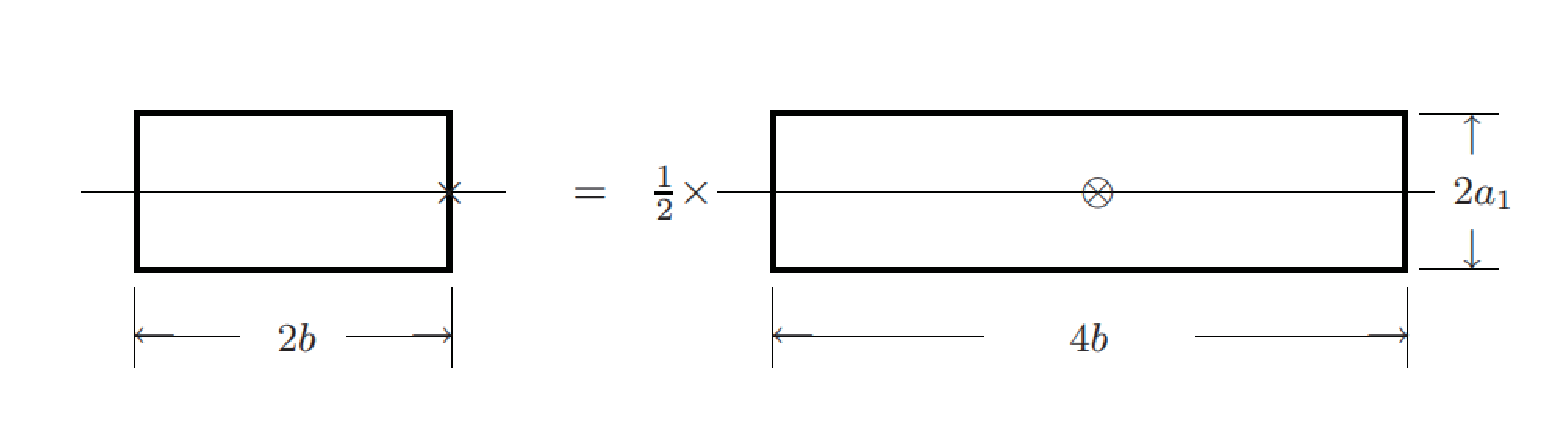
\includegraphics[scale=0.4]{chpt3/figs/fig3.20.eps}
	\caption{采用叠加技术,一个长度为$2b$的轴对称螺管末端磁场可以按照同样尺寸但长度$4b$的螺管的中心场的一半计算。}
\end{figure}

\begin{figure}
	\centering
	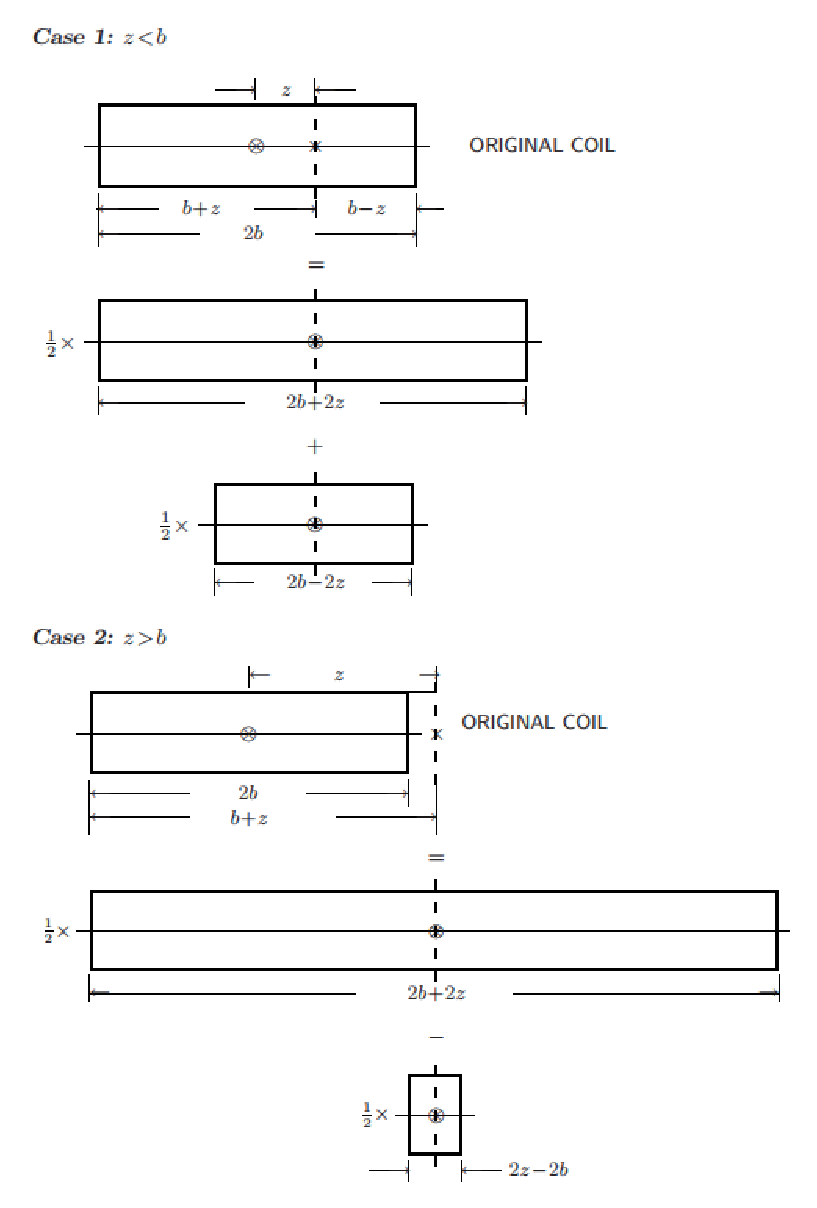
\includegraphics[scale=0.7]{chpt3/figs/fig3.21.eps}
	\caption{处理偏离轴心点的叠加技术。}
\end{figure}

\newpage

\subsection{讨论3.5:混合磁体}
混合磁体包括两个不同种类的轴向对齐且居中的电磁体:大功率水冷磁体置于超导磁体(SCM)的室温孔内。
1960年代,国家磁体实验室(NML)的Montgomery等人证实它是获得高达$\sim 25\ \mathrm{T}$直流磁场的一种方法[3.11]。
这个磁场是当时可用电源$9\ \mathrm{MW}$所能支持Bitter磁体实现的最高直流场。
此后30年,磁体实验室设计、制造和运行了多台混合磁体,为混合磁体技术做出了贡献[3.12–3.18]。

\textbf{A. 代表性的混合磁体设施}

现在多有个混合磁体在运行。下面以开始运行的时间为序,对几个代表性的混合磁体作简要介绍。

\textbf{\kaishu 高场磁体实验室,Radboud大学}

位于Nijmegen的高场磁体实验室(High Field Magnet Laboratory,HFML)自1977年起,运行了两个25.4 T [3.12] 和 32 T [3.14, 3.15]的混合磁体,由6-MW电源供电[3.19]。他们最新安装了20-MW电源[3.20]并升级了水冷磁体,2012年它的45 T混合磁体投入运行。

\textbf{\kaishu 高场实验室,Tohoku大学}

使用7.5 MW电源,自1983年开始运行。高场实验室(High Field Laboratory)已将其“湿”混合磁体
替换为“干”式,产生了30T的磁场[3.23]。

For a facility hybrid magnet that must undergo many field-sweep sequences, its
SCM should ideally be dry and of HTS. A dry cryostat avoids loss of liquid cryogen
after a trip in its water-cooled magnet;
高温超导磁体相比低温超导磁体,可以承受更大的由交流损耗产生的运行温度的温升。
第4章将讨论两个设计/运行选项,该选项使得在混合磁体运行条件下甚至一个干式高温超导磁体都能可靠运行:
1)超导磁体腔内放置大量固体制冷工质;2)采用低温环形器(cryocirculator,讨论4.7)而不是制冷机作为SCM的初级冷源。

\textbf{\kaishu Grenoble高场实验室}

Grenoble磁体实验室在1987年开始运行混合磁体[3.24]。
他们最近的24-MW电源[3.25]为40-T混合磁体做保障[3.26]。

\textbf{\kaishu 磁体实验室,国家材料科学研究院}

位于Tsukuba的国家材料科学研究院的磁体实验室(Magnet Laboratory at the National Institute of Materials Science)自1995年开始运行混合磁体。他们有一台17-MW电源,用于运行30–35 T混合磁体[3.27]。

\textbf{\kaishu 国家高场实验室(NHMFL)}

Florida州立大学的国家强磁场实验室的45-T混合磁体[3.28, 3.29]产生了世界上最大的直流磁场。当前,水冷磁体产生了
34T,SCM产生了11T [3.30]。该SCM下文会详细讨论。

\textbf{B. NHMFL 45 T混合磁体}

图3.22给出了NHMFL的45T混合磁体的水冷磁体、SCM和一些附件的剖面图[3.31。
水冷磁体有四个嵌套线圈,在24MW功率下产生31T的中心场。
SCM由三个线圈A、B、C组成,运行于1.8K,最初产生了14T磁场,但现在运行在11T[3.30];
水冷磁体经修改设计,可以在30MW功率下产生34T磁场。
系统包括超流液氦杜瓦,SCM杜瓦通过管道与之相连,图的中部右侧可见。
\begin{figure}[htbp]
	\centering
	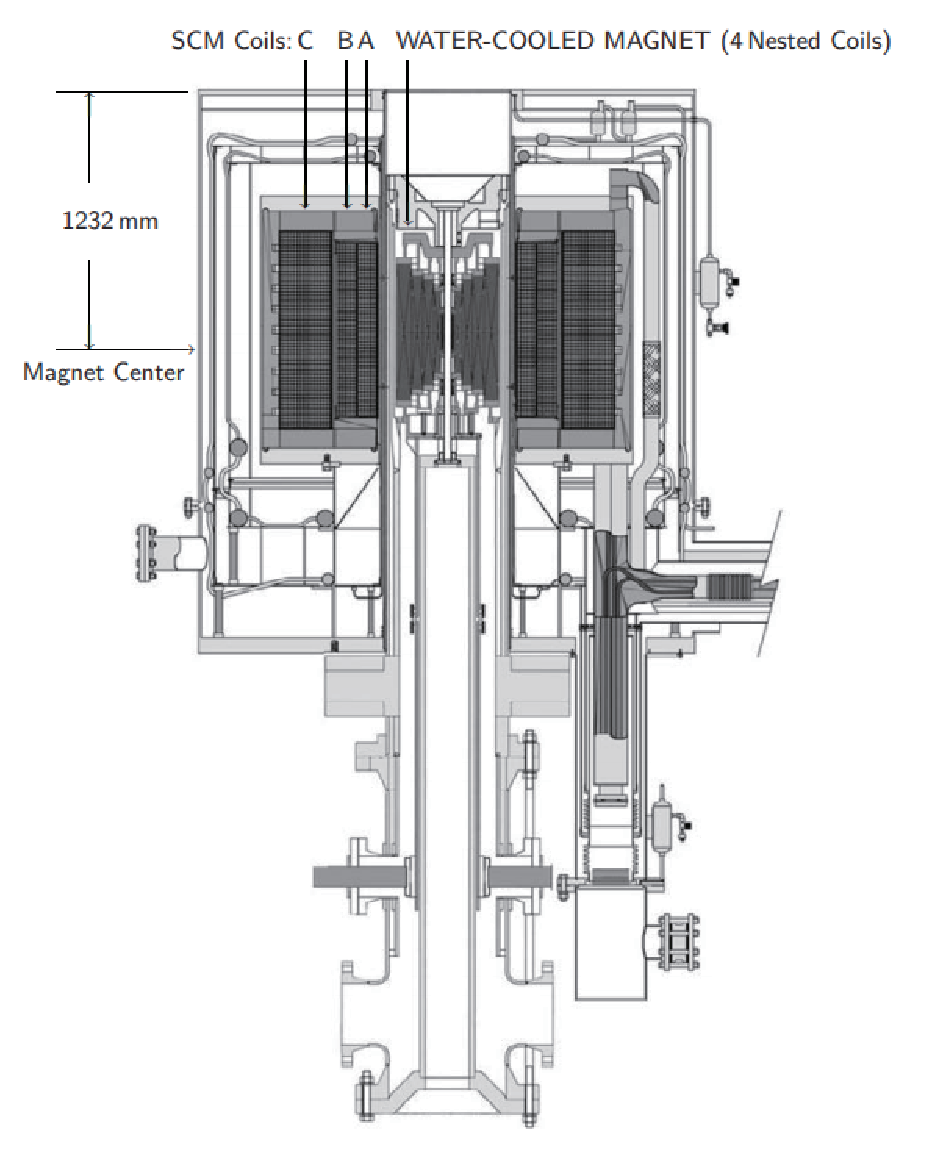
\includegraphics[scale=0.7]{chpt3/figs/fig3.22.eps}
	\caption{NHMFL 45 T混合磁体剖面图。}
\end{figure}

%%%%% 参数表
\colorbox{red}{这里缺一个参数表}

\textbf{\kaishu 45 T 混合超导磁体参数}

表3.3给出了45T混合SCM的关键参数[3.31]。这个SCM最突出的特征是它的三个线圈,
每一个都是由CICC导体(cable-in-conduit conductor)绕成的,CICC的更多细节,第6章会讨论。
两个内部的线圈A和B是层绕的,外部的线圈是由29个双饼线圈堆叠的。

\textbf{C. 混合磁体的工程挑战}

混合磁体很稀少,仅在大概五六个重点国家实验室内运行。
它不是一类采用常规方法制造的磁体,甚至制造周期要超过1年。
当然,它不是那种可以有一群工程师或物理学家在几个月就能造出来的。
因此,仅有很少的工程师实际参与到设计、制造和运行混合磁体中来。
它将两类磁体以很近的距离组合起来,一个运行于常温,另一个运行于液氦温度。两个磁体的电磁和机械是紧耦合的。
于是,除了每个磁体特定的工程问题,混合磁体还存在特有的重要设计和运行挑战:
处于低温的SCM的巨大的对处于室温的磁体机械结构的作用力,SCM杜瓦上最小的热负荷传导。
尽管本书的读者的大部分不会看到混合磁体本体,但它提供了多数磁体和低温工程师会发觉有指导意义的设计和运行要点。

关于混合磁体的一般话题在本节后面和第4/6/7/8张都会涉及,这些话题是基于MIT运行的35T混合磁体的[3.16–3.18]。

\textbf{D. 配置和独有特征}

混合磁体中,超导磁体总是置于水冷磁体(内插)外侧。在这个配置下,优化每一组件的特性。

\textbf{\kaishu 水冷磁体}
\begin{itemize}
	\item 在讨论3.2中已经证明,Bitter磁体的功率需求$P_B$正比于$a_1$和$[B_z(0, 0)]^2_B$ (方程3.116a),
	其中,$P_B$典型值为$6\sim 30\ \mathrm{MW}$。Bitter磁体相当耗电,最好对其整个体积进行优化:
	将其作为混合磁体的内插单元。
	不过,磁场越强,磁场对导体的磁应力越大,导体材料强度就该越强,而这一般意味着更大电阻。
	于是,$B_z(0, 0)\propto\sqrt{P}$ (方程3.113a)和$[B_z(0, 0)]_B\propto\sqrt{P_B}$ (方程3.116a)在高场时
	都是无效的。
	
	\item 常规金属比如“铜”没有“内秉”的场极限,不存在高于某个长就不能用它制造磁体的问题。
	但是,如上所述,由于强度高的材料需要更多的功率,等量的要求更多的冷量以匹配增加的焦耳热耗散,
	$30-40\ \mathrm{T}$一般认为是实际磁体设施的极限了。
\end{itemize}

\textbf{\kaishu 超导磁体}
\begin{itemize}
	\item 超导体都有明确的上临界场,超过了即失超。于是,最好将超导磁体放在混合磁体
	的低场部分:将它置于水冷磁体外侧。
	
	\item 总的存储磁能随磁体大小增加而增加,但对功率的需求——主要来自制冷——并不显著。
	$100\ \mathrm{MJ}$的磁体并不需要$100\ \mathrm{MW}$的电源,通常$10-100\ \mathrm{kW}$就足够了。
\end{itemize}

统筹考虑这些特征,我们就很自然的理解为什么混合磁体是内侧放水冷磁体,外部包围一个超导磁体了。

\textbf{作用力}

混合磁体的一个独特特征和需求源自内插磁体和SCM相互作用力。
如果两个磁体轴向和径向都是对齐的,特闷之间无相互作用力。
但是,他们场中心的相对错位导致很大的作用力。轴向错位产生使轴向对齐的轴向恢复力。
场中心的径向错位导致错位进一步增加,即失稳。
一般的,力是适中的;小心的设计和建造可以相对容易的应对此事。
不过,高性能湿冷内插磁体的失效是不可避免的。
若失效,比如当内插绕组短路,减少了产生的磁场,引起的场错位会突然产生很大的力。

为了控制故障力,结构上的需求是最重要的,其次是磁体的监控保护。由于两个磁体的磁耦合(互感),控保也很复杂。
很明显,每个磁体及其电源系统都必须有某种电保护以防止在哪里出错的时候损坏或损伤。
但还存在即使两个磁体分离后仍存在的强电耦合。第8章的问题8.3和8.4讨论线圈的一般监控细节以及混合磁体的特别问题。
\newpage

\subsection{讨论3.6:双饼 vs. 层绕}
两个磁体的绕制技术中,有一种被普遍成为“双饼”或简单的称为“饼”;另一种是“层绕”。
双饼线圈通常使用扁平带材绕成,有时也采用大的方截面或长方形截面导体(如CICC)绕成。
每一个双饼都是由一根连续的导体绕成的。双饼线圈的概念图如图3.23所示,双饼绕制的起点是导体的中点(图中的C处附近),
而层绕的话,起点在导体的一端(图中的A或B)。
因为每一个双饼线圈的绕组高度$(2b)$大约是导体宽度的2倍,所以一个实际的磁体需要多个双饼线圈,相邻线圈在径向
最外侧绕组直径范围内$(2a_2)$拼接起来。而层绕线圈是从一端到另一端连续绕制,从最里层到最外层一层一层绕成。两种技术的
优缺点下文将加以讨论。

\begin{figure}[htbp]
	\centering
	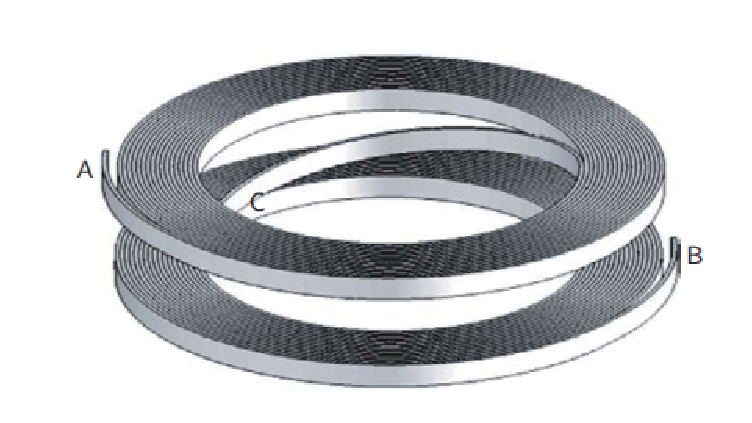
\includegraphics[scale=0.6]{chpt3/figs/fig3.23.eps}
	\caption{双饼线圈图示。为了清晰,上下饼分开了。图中这种双饼是由超导带材绕制的,点A和点B是连续导体的端头,而点C大约是带材的中点。}
\end{figure}

\textbf{优势和劣势}
\begin{enumerate}
	\item 对双饼线圈,对导体长度的要求低于层绕线圈。对小线圈,无接头的长度为$\sim 50\ \mathrm{m}$
	的导体就足够了。甚至对于大型磁体,$\sim 1-2\ \mathrm{km}$也够了。
	另一方面,对层绕线圈,单个线圈所需的无接头导体长度轻易超过$10\ \mathrm{km}$。
	由于长导体更难制造,所以如果考虑导体长度,饼式线圈优于层绕线圈。

	\item 饼式磁体一般要求很多双饼线圈,每一个双饼理想状态下应该是同一化的模块以构成磁体绕组的高度。
	这种模块化磁体方法,结合上面提及的导体长度要求,使得饼式线圈的制造更加简单(也更便宜)。
	同时,层绕线圈可能出现的绕制过程一个问题可能导致整个线圈导体不可用的情况在饼式线圈这里,
	只会影响到一个双饼的导体量。
	由于每个双饼的电磁性能和尺寸会存在微笑的不同,另一个饼式线圈技术的优点就是它让线圈置于
	其最适合位置的操作成为可能。

	\item 饼式线圈技术的一个明显的不足是它不可避免相邻双饼的连接。
	连接是制造的一个额外过程。由于连接必须随依绕组的形状,实施起来比单一导体焊接困难。
	或许对于运行更重要的是这些接头产生的焦耳热耗散——除非接头也是超导的。NMR和MRI磁体一般是要求超导接头的。
\end{enumerate}

\newpage

\subsection{问题3.3:亥姆霍兹线圈}
很多应用都希望有高均匀性的磁场。
一种被称为“Helmholtz coil”的简单布局可以在一个有限的区域内实现高均匀磁场。
它使用两个一致的空间上同轴但在磁场轴线($z$向)分开一定距离的的线圈(图3.24a);
两个线圈分别位于$z = d/2$和$z = −d/2$。通过调整间隔$d$,使得磁场中心处于($r=0,z=0$):
%3.121
\begin{equation}% 3.121
\frac{d^2H_z(0,z)}{dz^2}\mid_{z=0}=0
\end{equation}

a) 将两个线圈看成理想的“环”线圈,半径为$a$,证明当$d=a$时,在中心处有$dH^2_z(0, z)/dz^2 = 0$。
图3.24b中的实线给出了一个不满足方程3.121的$d$下的$H_z(0, z)$。

b) 证明两个线圈如果反极性,中心处会产生一个梯度场。
在$z=0$处计算$dH_z/dz$。(注意,当$d=a$时$d^3H_z(0,z)/dz^3 \neq 0$;$d^3H_z(0,z)/dz^3=0$要求$d=\sqrt{3}a$) 
此种相反电流的配置称为Maxwell线圈。图3.24b中的虚线给出了梯度线圈的$H_z(z)$。

\begin{figure}[htbp]
	\centering
	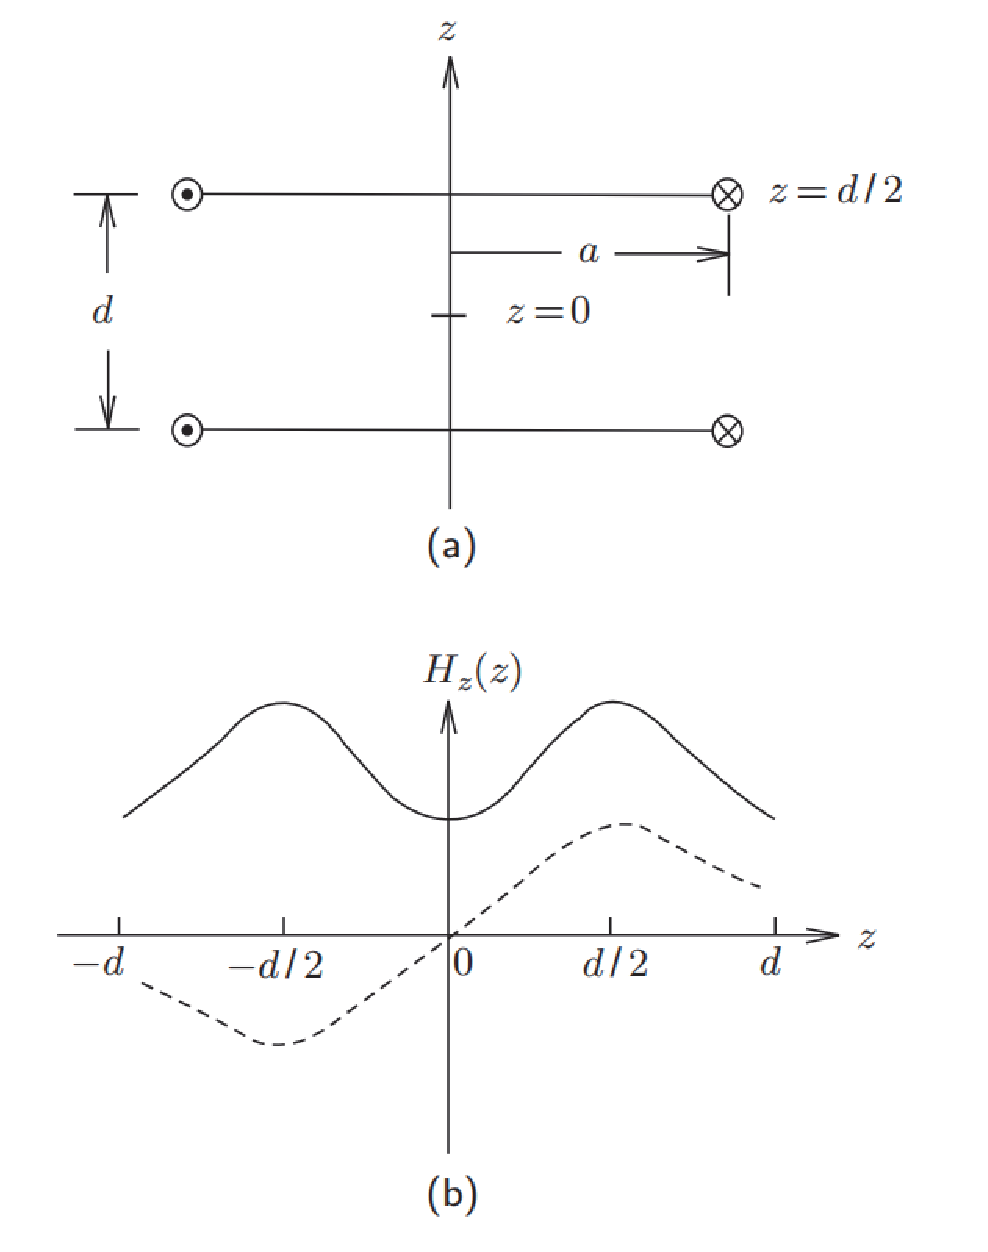
\includegraphics[scale=0.4]{chpt3/figs/fig3.24.eps}
	\caption{(a)理想Helmholtz线圈布局;(b)均匀场下的$H_z(0,z)$(实线)和梯度场下的$H_z(0,z)$(虚线)}
\end{figure}

\subsubsection{问题3.3之解}
a) 位于下方$z=−d/2$处环产生的轴向($r =0$)磁场的$z$分量可由方程3.3a给出:
% 方程
\begin{equation}% page139
H_z(0,z)=\frac{a^2I}{2[a^2+(z+\frac{d}{2})^2]^\frac{3}{2}}
\end{equation}

加上位于上面$z=d/2$处的线圈的磁场,有:
%S3.1
\begin{equation}% S3.1
H_z(0,z)=\frac{a^2I}{2}\left\{\frac{1}{[a^2+(z+\frac{d}{2})^2]^\frac{3}{2}}+\frac{1}{[a^2+(z-\frac{d}{2})^2]^\frac{3}{2}}\right\}
\end{equation}

将S3.1给出的方程$H_z(z)$对$z$微分,有:
% 方程
\begin{equation}
\frac{d^2H_z(0,z)}{dz}=\frac{3a^2I}{2}\left\{{-\frac{(z+\frac{d}{2})}{[a^2+(z+\frac{d}{2})^2]^\frac{5}{2}}-\frac{(z-\frac{d}{2})}{[a^2+(z-\frac{d}{2})^2]^\frac{5}{2}}}\right\}
\end{equation}

注意,由于对称性,$dH_z(0,z)/dz=0$在$z=0$处对任意$a$成立。

对S3.1二次微分有:
% 方程
\begin{equation}
\frac{d^2H_z(0,z)}{dz^2}=\frac{3a^2I}{2}\left\{{-\frac{a^2-4(z+\frac{d}{2})^2}{[a^2+(z+\frac{d}{2})^2]^\frac{7}{2}}}
-\frac{a^2-4(z-\frac{d}{2})^2}{[a^2+(z-\frac{d}{2})^2]^\frac{7}{2}}\right\}
\end{equation}

如果$d = a$,在$z = 0$处二阶导数为零。
这种同轴放置两个同一线圈,且其距离等于线圈半径的做法产生了一个高均匀场区域。
这里的二阶分析是MRI和其他要求高空间均匀性磁场磁体设计的重要准则之一。The second derivative is zero at  if . 

b) 对这个系统,下方线圈的电流极性反转,有:
% s3.2
\begin{equation}% S3.2
H_z(0,z)=\frac{a^2I}{2}\left\{{-\frac{1}{[a^2+(z+\frac{d}{2})^2]^\frac{3}{2}}+\frac{1}{[a^2+(z-\frac{d}{2})^2]^\frac{3}{2}}}\right\}
\end{equation}

根据对称性,$H_z(z=0)=0$。对S3.2依$z$求导,有:
%s3.3
\begin{equation}% S3.3
\frac{dH_z(0,z)}{dz}=\frac{3a^2I}{2}\left\{{\frac{(z+\frac{d}{2})}{[a^2+(z+\frac{d}{2})^2]^\frac{5}{2}}-\frac{(z-\frac{d}{2})}{[a^2+(z-\frac{d}{2})^2]^\frac{5}{2}}}\right\}
\end{equation}

在$z=0$处计算S3.3,有:
%方程
\begin{equation}
\frac{dH_z(0,z)}{dz}\mid_0=\frac{3a^2Id}{2[a^2+(z+\frac{d}{2})^2]^\frac{5}{2}}
\end{equation}

这种放置两个同一但电流方向相反的线圈产生梯度场的方法是要求中平面梯度场磁体设计中使用的基本法则。
MRI系统中使用的脉冲磁体产生梯度场(从成像中提取空间信息)就是一个例子。
\newpage

\subsection{问题3.4:亥姆霍兹线圈分析——另一种方法}
这一节,我们使用方程3.16a和3.22分析问题3.3中的Helmholtz线圈。

证明,两个半径为$a$、分别位于$\xi(\equiv z/a)=+0.5$ 和$\xi=−0.5$的“环”线圈1和2组成的Helmholtz对,
轴向场在其中心($\xi=0$)的二阶导数$d^2 h_z(0)/d\xi^2|_{1/2}$可以表示为$\xi^{2n}$的级数且随着
项数增加而收敛于0。由于并未计算每一个线圈在$\xi=0$的值,所以3.17b的简化表达式不能用。


使用最高项第20项计算$d^2 h_z(0)/d\xi^2|_{1/2}$。注意到$E_2(1, 0)\cdots E_{10}(1, 0)$已由3.28给出。
导出$E_2(1, 0)\cdots E_{10}(1, 0)$的技术也可以用于从3.15b导出$E_{12}(\alpha, 0)\cdots E_{20}(\alpha, 0)$,$f_{12}(\alpha,\beta)\cdots f_{20}(\alpha,\beta)$在附录IB中有。
在极限$\beta\rightarrow 0$下,将$1/(1+\beta^2)^{19.5}$展开至$\beta^{20}$项,有:
%3.122
\begin{equation}% 3.122
\frac{1}{(1+\beta)^{19.5}}=1-\frac{39}{2}\beta^2+\frac{39}{2}\cdot\frac{41}{2}\frac{\beta^4}{2!}-\frac{39}{2}\cdot\frac{41}{2}\cdot\frac{43}{2}\frac{\beta^6}{3!}+\cdots
+\frac{39}{2}\cdot\frac{41}{2}\cdot\frac{43}{2}\cdot\frac{45}{2}\cdot\frac{47}{2}\cdot\frac{49}{2}\cdot\frac{51}{2}\cdot\frac{53}{2}
\cdot\frac{53}{2}\cdot\frac{57}{2}\frac{\beta^{20}}{10!}
\end{equation}

$E_{12}(\alpha, 0)\cdots E_{20}(\alpha, 0)$类似于方程3.21中的$E_{2}(\alpha, 0)\cdots E_{10}(\alpha, 0)$,我们有:
%3.123
\begin{equation}% 3.123a
E_{12}(\alpha,0)=\frac{7\cdot11\cdot13}{2^{12}}\cdot\frac{(\alpha^{12}-1)}{\alpha^{12}\ln\alpha}=\frac{1001(\alpha^{12}-1)}{4096\alpha^{12}\ln\alpha}
\end{equation}
\begin{equation}% 3.123b
E_{14}(\alpha,0)=-\frac{5\cdot9\cdot11\cdot13}{2^{12}\cdot7}\cdot\frac{(\alpha^{14}-1)}{\alpha^{14}\ln\alpha}=-\frac{6435(\alpha^{14}-1)}{28672\alpha^{14}\ln\alpha}
\end{equation}
\begin{equation}% 3.123c
E_{16}(\alpha,0)=\frac{5\cdot9\cdot11\cdot13\cdot17}{2^{19}}\cdot\frac{(\alpha^{16}-1)}{\alpha^{16}\ln\alpha}=\frac{109395(\alpha^{16}-1)}{524288\alpha^{16}\ln\alpha}
\end{equation}
\begin{equation}% 3.123d
E_{18}(\alpha,0)=-\frac{5\cdot11\cdot13\cdot17\cdot19}{2^{17}\cdot3^2}\cdot\frac{(\alpha^{18}-1)}{\alpha^{18}\ln\alpha}=-\frac{230945(\alpha^{18}-1)}{1179648\alpha^{18}\ln\alpha}
\end{equation}
\begin{equation}% 3.123e
E_{20}(\alpha,0)=\frac{3\cdot7\cdot11\cdot13\cdot17\cdot19}{2^{20}\cdot5}\cdot\frac{(\alpha^{20}-1)}{\alpha^{20}\ln\alpha}=\frac{969969(\alpha^{20}-1)}{5242880\alpha^{20}\ln\alpha}
\end{equation}

在极限$\alpha\rightarrow 1$时,方程3.123a-3.123e成为:
%3.124
\begin{equation}% 3.124a
E_{12}(1,0)=\frac{3003}{1024}=\frac{3\cdot7\cdot11\cdot13}{2^{10}}=\frac{3\cdot5\cdot7\cdot9\cdot11\cdot13}{2\cdot4\cdot6\cdot8\cdot10\cdot12}\simeq2.933
\end{equation}
\begin{equation}% 3.124b
E_{14}(1,0)=-\frac{6435}{2048}=-\frac{5\cdot9\cdot11\cdot13}{2^{11}}=-\frac{3\cdot5\cdot7\cdot9\cdot11\cdot13\cdot15}{2\cdot4\cdot6\cdot8\cdot10\cdot12\cdot14}\simeq-3.142
\end{equation}
\begin{equation}% 3.124c
E_{16}(1,0)=\frac{109395}{32768}=\frac{5\cdot9\cdot11\cdot13\cdot17}{10^{15}}=\frac{3\cdot5\cdot7\cdot9\cdot11\cdot13\cdot15\cdot17} {2\cdot4\cdot6\cdot8\cdot10\cdot12\cdot14\cdot16}\simeq3.338
\end{equation}
\begin{equation}% 3.124d
E_{18}(1,0)=-\frac{230945}{65536}=\frac{5\cdot11\cdot13\cdot17\cdot19}{10^{16}}=-\frac{3\cdot5\cdot7\cdot9\cdot11\cdot13\cdot15\cdot17\cdot19} {2\cdot4\cdot6\cdot8\cdot10\cdot12\cdot14\cdot16\cdot18}\simeq-3.524
\end{equation}
\begin{equation}% 3.124e
E_{20}(1,0)=\frac{969969}{262144}=\frac{3\cdot7\cdot11\cdot13\cdot17\cdot19}{10^{18}}=\frac{3\cdot5\cdot7\cdot9\cdot11\cdot13\cdot15\cdot17\cdot19\cdot21} {2\cdot4\cdot6\cdot8\cdot10\cdot12\cdot14\cdot16\cdot18\cdot20}\simeq3.700
\end{equation}

\subsubsection{问题3.4之解}
位于$\xi=+0.5$的线圈1贡献的$d^2h_z(\xi)/dxi^2$在 $xi=0$时$d^2h_z(0)/d\xi^2|_{1/2}$由方程3.16a给出:
%s4.1
\begin{equation}% S4.1
\frac{d^2h_z(0)}{d\zeta^2}\mid_{\frac{1}{2}}=2E_2(1,0)+12E_4(1,0)\times(0.5)^2+30E_6(1,0)\times(0.5)^4+56E_8(1,0)\times(0.5)^6+90E_{10}(1,0)\times(0.5)^8
+132E_{12}(1,0)\times(0.5)^{10}+182E_{14}(1,0)\times(0.5)^{12}+240E_{16}(1,0)\times(0.5)^{14}+306E_{18}(1,0)\times(0.5)^{16}+380E_{20}(1,0)\times(0.5)^{18}+\cdots
\end{equation}

由于线圈2(位于$\xi=−0.5$)和位于$\xi=0.5$的线圈1在$\xi=0.5$处给出树枝上相同的$d^2\xi_z/d\xi^2$,我们有:
%s4.2
\begin{equation}% S4.2
\frac{d^2h_z(0)}{d\zeta^2}\mid_{\frac{1}{2}}=4(-\frac{3}{2})+24(\frac{15}{8})(0.5)^2+60(-\frac{35}{16})(0.5)^4+112(\frac{315}{128})(0.5)^6+180(-\frac{693}{256})(0.5)^8
+264(\frac{3003}{1024})(0.5)^{10}+264(-\frac{6435}{2048})(0.5)^{12}+480(\frac{109395}{32768})(0.5)^{14}+612(-\frac{230945}{65536})(0.5)^{16}
+760(\frac{969969}{262144})(0.5)^{18}+\cdots
\end{equation}

随着项数增加,我们计算方程S4.2:
%方程
\begin{eqnarray}
\frac{d^2h_z(0)}{d\zeta^2}\mid_{\frac{1}{2}}&=&-6\ (only E_2)\\
&=&5.25  \ (through\ E_4)\\
&\simeq& -2.9531\   (through\ E_6)\\
&\simeq& 1.3535\ (through\ E_8)\\
&\simeq& -0.5499\   (through\ E_{10})\\
&\simeq& 0.2062 \  (through\ E_{12})\\
&\simeq& -0.0730\   (through\ E_{14})\\
&\simeq& 0.0248 \  (through\ E_{16})\\
&\simeq&-0.0081\   (through\ E_{18})\\
&\simeq& 0.0026 \  (through\ E_{20})
\end{eqnarray}


由上可知,随着高次项的加入, $d^2h_z(0)/d\xi^2|_{1/2}\rightarrow 0$。
注意到,对置于$\xi=0$的一个孤立环线圈: $d^2h_z(0)/d\xi^2=−3$。
\newpage


\subsection{问题3.5:一个空间均匀磁体的分析}
\begin{figure}[htbp]
	\centering
	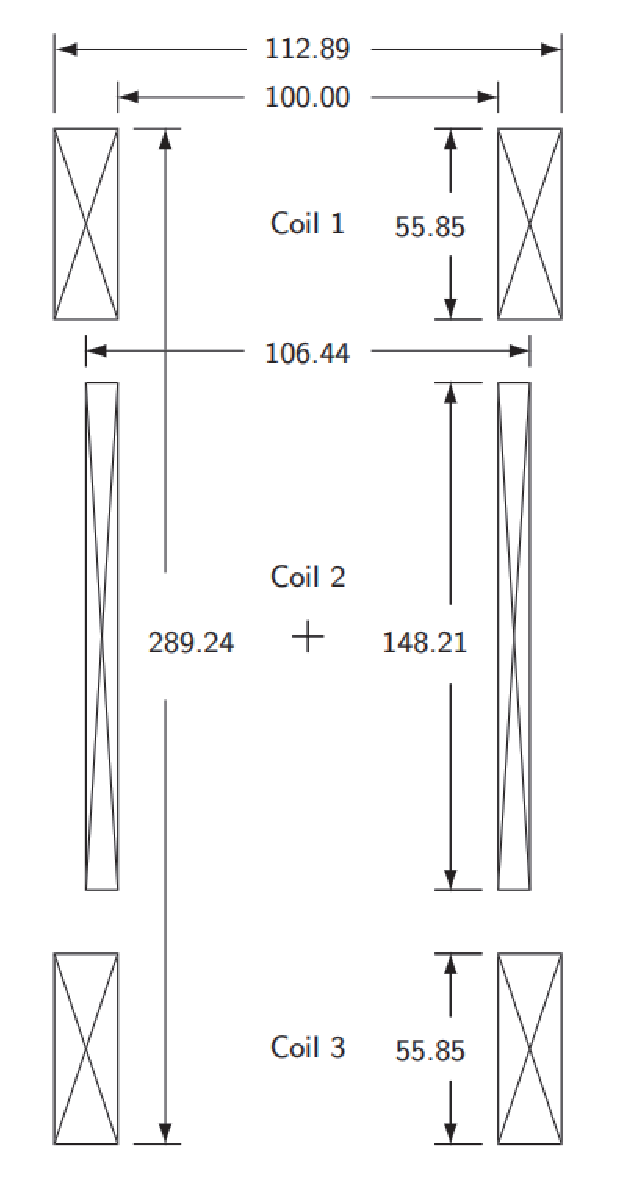
\includegraphics[scale=0.5]{chpt3/figs/fig3.25.eps}
	\caption{三个线圈组成的磁体,以mm为单位}
\end{figure}
图3.25给出了一个由三个线圈组成的空间均匀磁体的结构剖面。
线圈1和线圈3是完全一样的,分别位于中间线圈2的上下方,
用以加强中心场$(0,0)$的均匀性。
关键尺寸(mm为单位)已在图中标注。
每个线圈的$2a_1$都是$100\ \mathrm{mm}$,每个线圈的总电流密度均为
$\lambda J =2.5147×108 A/m^2$。
表格3.4给出了使用Bobrov程序计算得到的场参数[3.32]。
%% 表格3.4


\begin{figure}[htbp]
	\centering
	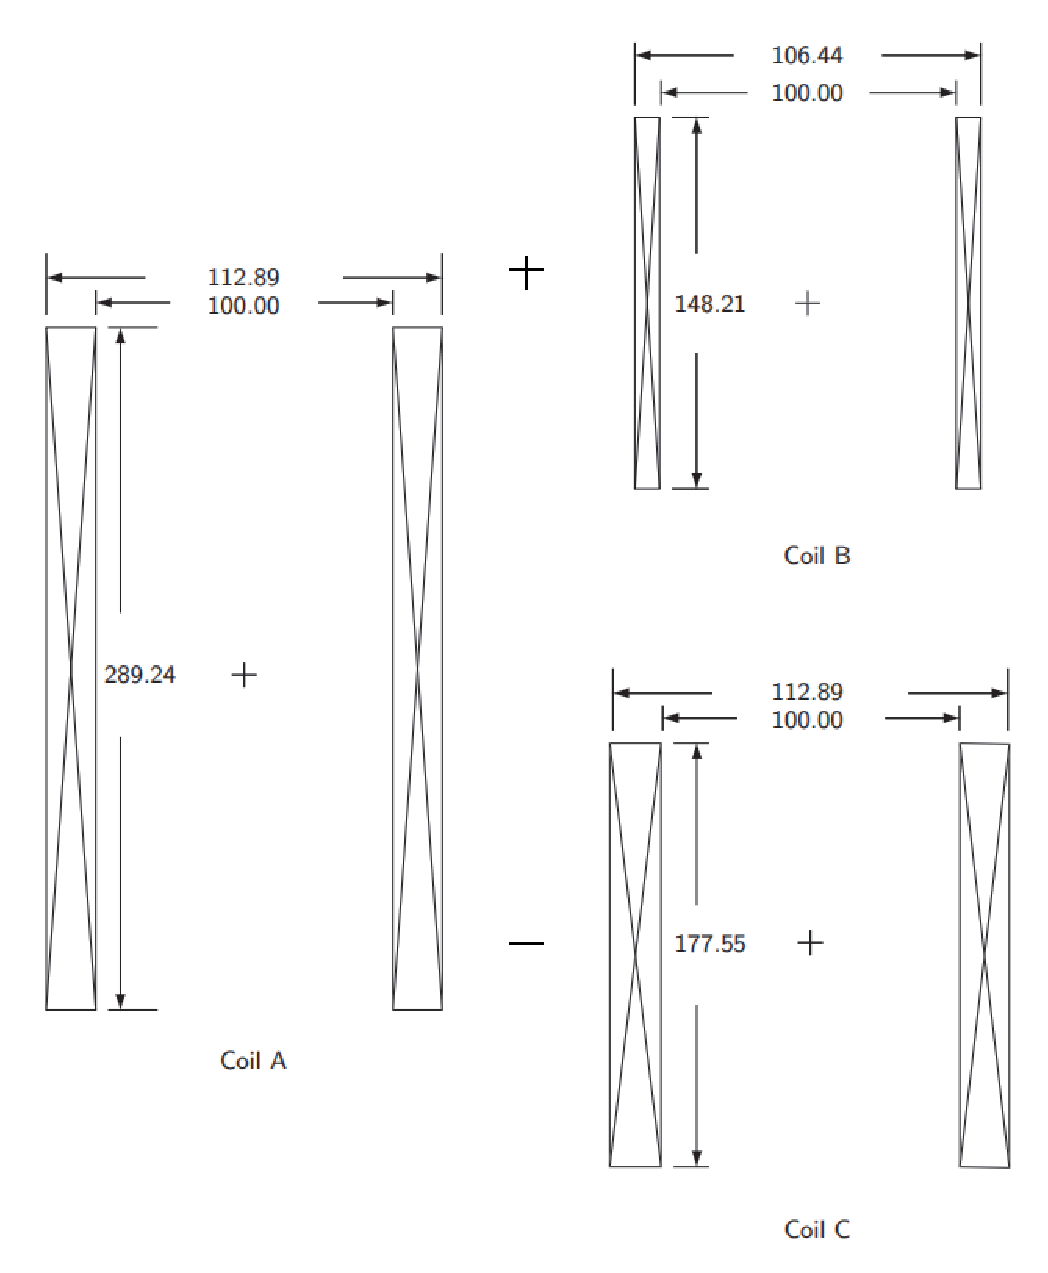
\includegraphics[scale=0.7]{chpt3/figs/fig3.26.eps}
	\caption{图3.25中的三个线圈表示为A、B、C,每个线圈的中心都位于磁体中心。线圈C的符号表示
		它的载流是与A和B反向的。以mm为单位}
\end{figure}
图3.26给出的是同一个磁体,线圈用A、B和C表示,各线圈的中心都是$(0,0)$。
线圈A从线圈1延伸至线圈3,还包括中间的两个间隙。线圈B与线圈2一致。
因为这个新的表示法中线圈2被线圈A和线圈B代表了2次,
所以加入与线圈A和B电流相反的线圈C,以减掉1个线圈2以及那两个间隙。

a) 证明,如果线圈A、B和C的总电流密度都是$\lambda J$,图3.26的线圈配置和原线圈配置给出相同的中心场;
\begin{equation} %3.125
B_0 = 1.000 T=\mu_0\lambda J a_1[F_A(\alpha,\beta)+F_B(\alpha,\beta)-F_C(\alpha,\beta)]
\end{equation}

b) 应用方程3.14和3.17,并使用手持科学计算器,计算本磁体的$d^2B/dz^2|_0$和$d^4B/dz^4|_0$。
计算值应该可表3.4使用程序计算的结果吻合。

\subsubsection{问题3.5之解}
表3.5列出了线圈A、B和C的$\alpha$和$\beta$的近似值。采用这些数值,我们得到:

%表格3.5

%计算的F
\begin{eqnarray}% page144
F_A(\alpha,\beta)&=0.12094421\\
F_B(\alpha,\beta)&=0.05287933\\
F_C(\alpha,\beta)&=0.11053327
\end{eqnarray}

a)从方程3.125,我们有:
%%
\begin{equation}% page144
\begin{split}
B_0=&(4\pi\times 10^{-7}H/m)(2.5147\times 10^8 A/m^2)(5\times 10^{-2}m)\\
&\times(0.12094421+0.05287933-0.11053327)=1.000 T
\end{split}
\end{equation}

b)将$\alpha$和$\beta$代入方程3.14a和3.14b1,我们有:
%%
 \begin{eqnarray}% page144
F(\alpha,\beta)E_2(\alpha,\beta)_A=-0.002277367;F(\alpha,\beta)E_4(\alpha,\beta)_A=-0.000315757\\
F(\alpha,\beta)E_2(\alpha,\beta)_B=-0.007938543;F(\alpha,\beta)E_4(\alpha,\beta)_B=-0.001737981\\
F(\alpha,\beta)E_2(\alpha,\beta)_C=-0.010216278;F(\alpha,\beta)E_4(\alpha,\beta)_C=-0.002133593
\end{eqnarray}

当所有线圈都有相同的$a_1$和$\lambda J a_1$时,方程3.18成为:
\begin{equation}% S5.1
h_\zeta(\zeta)=1+\frac{\sum_{k}^{j=1}F(\alpha_j,\beta_j)E_2(\alpha_j,\beta_j)}{\sum_{k}^{j=1}F(\alpha_j,\beta_j)}\zeta^2+\cdots
\end{equation}

 \begin{equation}% page144
E_2(\alpha,\beta)=\frac{F(\alpha,\beta)E_2(\alpha,\beta)_A+F(\alpha,\beta)E_2(\alpha,\beta)_B-F(\alpha,\beta)E_2(\alpha,\beta)_C}{F(\alpha,\beta)_A+F(\alpha,\beta)_B-F(\alpha,\beta)_C}
=\frac{-0.002277367-0.007938543+0.010216278}{0.120924421+0.05287933-0.11053327}=0.000005822
E_4(\alpha,\beta)=\frac{-0.000315757-0.001737981+0.002132363}{0.6329027}=0.001261725
\end{equation}

于是我们有:
\begin{eqnarray}% page144
\frac{d^2B}{dz^2}\mid0=2E_2(\frac{B_0}{a_{1}^{2}})=2(0.000005822)\frac{1.000T}{(5 cm)^2}=0.4658\times10^{-6}T/cm^2\\
\frac{d^4B}{dz^4}\mid0=24E_4(\frac{B_0}{a_{1}^{4}})=24(0.001261725)(\frac{(1.000T)}{(5 cm)^4})=4.8453\times10^{-5}T/cm^4
\end{eqnarray}

这些数值与表3.4给出的事实上是一致的,尽管需要我们勤奋的计算至第九位小数。

值得注意的是,这里呈现的分析对计算给定此题设计的场梯度是很有用的,尽管乏味。
这里给出的分析形式对设计空间高均匀性磁体并不实用;它只是对开发个人的设计程序很有用。
\newpage


\subsection{问题3.6:直角坐标下的场展开}
在由图3.4定义的球坐标$(r, \theta,\phi)$下,
由嵌套线圈组成磁体产生的在无源子由空间的$z$向磁场$H_z$可由方程3.9表示:

证明,笛卡尔坐标系下$H_z(r, \theta,\phi)$的表达式$H_z(x, y, z)$在$n=0, 1, 2$分别为:
%%3.126
\begin{equation}% 3.126a
n=0\ H_z(x,y,z)=A_{0}^{0}
\end{equation}
\begin{equation}
n=1\ H_z(x,y,z)=A_{0}^{0}+2zA_{1}^{0}+3(A_{1}^{1}x+B_{1}^{1}y)
\end{equation}
\begin{equation}
\begin{split}
n=2\ H_z(x,y,z)=&A_{0}^{0}+2zA_{1}^{0}+3(A_{1}^{1}x+B_{1}^{1}y)\\
&+\frac{3}{2}A_{2}^{0}(2z^2-x^2-y^2)+12z(A_{2}^{1}x+B_{2}^{1}y)\\
&+15[A_{2}^{2}(x^2-y^2)+2B_{2}^{2}xy]
\end{split}
\end{equation}


\subsubsection{问题3.6之解}
球坐标参数$r, u = \cos\theta, s = \sin\theta, \sin\phi,\cos\phi$用$x,y,z$表示为:

%%S6.1
 \begin{eqnarray}% S6.1a
r=\sqrt{x^2+y^2+z^2}\\
u=\cos\theta=\frac{z}{\sqrt{x^2+y^2+z^2}}\\
s=\sin\theta=\frac{\sqrt{x^2+y^2}}{\sqrt{x^2+y^2+z^2}}\\
\sin\varphi=\frac{y}{\sqrt{x^2+y^2}}\\
\cos\varphi=\frac{x}{\sqrt{x^2+y^2}}
\end{eqnarray}

方程3.9与S6.1a-S6.1e分别对$n=0,1,2$联立,有:
\begin{equation}% S6.2a
\begin{split}
H_z(x,y,z)=&\sum_{0}^{m=0}r^0(1+0)P_{0}^{0}(u)(A_{0}^{0}\cos0 +B_{0}^{0}\sin 0)\\
=&(1)(1)(1)(A_{0}^{0})
\end{split}
\end{equation}

对$n=0$,我们有:
 \begin{equation}% 3.126a
H_z(x,y,z)=A_{0}^{0}
\end{equation}

注意到,$A_0^0$表示磁体中心场$H_z(0, 0, 0)$。
\begin{equation}% s6.3a
\begin{split}
H_z(x,y,z)=&\sum_{1}^{m=0}r^1(2+m)P_{1}^{m}(A_{1}^{m}\cos m\varphi+B_{1}^{m}\sin m\varphi)\\
=&r^1(2+0)P_{1}^{0}(A_{1}^{0})+r^1(2+1)
P_{1}^{1}(A_{1}^{1}\cos\varphi+B_{1}^{1}\sin\varphi)\\
=&2ruA_{1}^{0}+3rs(A_{1}^{1}\cos\varphi+B_{1}^{1}\sin\varphi)\\
=&2\sqrt{x^2+y^2+z^2}\frac{z}{\sqrt{x^2+y^2+z^2}}A_{1}^{0}\\
&+3\sqrt{x^2+y^2+z^2}\frac{\sqrt{x^2+y^2}}{\sqrt{x^2+y^2+z^2}}\left(\frac{A_{1}^{1}x+B_{1}^{1}y}{\sqrt{x^2+y^2}}\right)\\
=&2zA_{1}^{0}+3(A_{1}^{1}x+B_{1}^{1}y)
\end{split}
\end{equation}

于是,对最大为1的$n$值,我们有:
%%3.126b
\begin{equation}% 3.126b
H_z(x,y,z)=A_{0}^{0}+zA_{1}^{0}+3(A_{1}^{1}x+B_{1}^{1}y)
\end{equation}

注意,$H_z(x, y, z)$含有仅随着$z,x,y$变化的项。

%%S6.4
 \begin{equation}% S6.4
 \begin{split}
H_z(x,y,z)=&\sum_{2}^{m=0}r^2(3+m)P_{2}^{m}(A_{2}^{m}\cos m\varphi+B_{2}^{m}\sin m\varphi)\\
=&r^2(3+0)P_{2}^{0}(A_{2}^{0})+r^2(3+1)P_{2}^{1}
(A_{2}^{1}\cos\varphi+B_{2}^{1}\sin\varphi)\\
&+r^2(3+2)P_{2}^{2}(A_{2}^{2}\cos 2\varphi+B_{2}^{2}\sin 2\varphi)
 \end{split}
\end{equation}

\begin{equation}% S6.4b
\begin{split}
H_z(x,y,z)=&3(x^2+y^2+z^2)\frac{1}{2}\left(\frac{2z^2-x^2-y^2}{x^2+y^2+z^2}\right)A_{2}^{0}\\
&+4(x^2+y^2+z^2)\frac{3z\sqrt{x^2+y^2}}{x^2+y^2+z^2}
\left(A_{2}^{1}\frac{x}{\sqrt{x^2+y^2}}+B_{2}^{1}\frac{y}{\sqrt{x^2+y^2}}\right)\\
&+5(x^2+y^2+z^2)\frac{3(x^2+y^2)}{x^2+y^2+z^2}\left[A_{2}^{2}(\frac{2x^2}{x^2+y^2}-1)+B_{2}^{2}\frac{2xy}{x^2+y^2}\right]\\
=&\frac{3}{2}A_{2}^{0}(2z^2-x^2-y^2)\\
&+12z(A_{2}^{1}x+B_{2}^{1}y)+15[A_{2}^{2}(x^2-y^2)+2B_{2}^{2}xy]
\end{split}
\end{equation}

累加方程S6.2b, S6.3b和S6.4b,我们得到对最大为2的$n$值情况:
\begin{equation}% 3.126c
\begin{split}
H_z(x,y,z)=&A_{0}^{0}+2zA_{1}^{0}+3(A_{1}^{1}x+B_{1}^{1}y)\\
&+\frac{3}{2}A_{2}^{0}(2z^2-x^2-y^2)+12z(A_{2}^{1}x+B_{2}^{1}y)\\
&+15[A_{2}^{2}(x^2-y^2)+2B_{2}^{2}xy]
\end{split}
\end{equation}

注意到,当对$n=0,1,2$计算$H_z(x, y, z)$时,它包含随$x, y, z, z^2, x^2, y^2, zx, zy$和$xy$变化的项。
\newpage

\subsection{问题3.7:Notched螺管}
Helmholtz线圈的准则——关于螺管中心对称放置载流元以在中心区域产生空间均匀场——是notched螺管线圈设计的基本准则。
很多MRI和NMR磁体都是notched螺管设计的变种。

对一个简单螺管,绕组内半径$a_1$,外半径$a_2$,总长度$2b$,总电流密度$\lambda J$。
回想到前面方程3.13a和3.13b给出中心轴向场$H_0\equiv H_z(0, 0)$,有:
%%3.13a/b
 \begin{equation}% 3.13a
H_0=\lambda Ja_1F(\alpha,\beta)
\end{equation}
\begin{equation}% 3.13b
F(\alpha,\beta)=\beta\ln\left(\frac{\alpha+\sqrt{\alpha^2+\beta^2}}{1+\sqrt{1+\beta^2}}\right)
\end{equation}

考虑到对称性以及前面讨论3.4给出的叠加技术,证明
如图3.27所示的具有均匀电流密度$\lambda J$的notched螺管的$H_z(0, z_1)$的表达式为:
%%3.127
\begin{equation}% 3.127
\begin{split}
H_z(0,z_1)=&\frac{1}{2}\lambda a_1\left[F(\alpha_1,\beta_1+\gamma_1)+F(\alpha_1,\beta_1-\gamma_1)\right]\\
&-\frac{1}{2}\lambda Ja_3
\left[F(\alpha_2,\beta_2+\gamma_2)+F(\alpha_2,\beta_2-\gamma_2)\right]
\end{split}
\end{equation}

式中,$\alpha_1=a_2/a_1,\beta_1=b_1/a_1,\gamma_1=z_1/a_1,\alpha_2=a_2/a_3,\beta_2=b_2/a_3,\gamma_2=z_1/a_3$。螺管参数$a_1, a_2, a_3, b_1, b_2$如图3.27的定义。
\begin{figure}[htbp]
	\centering
	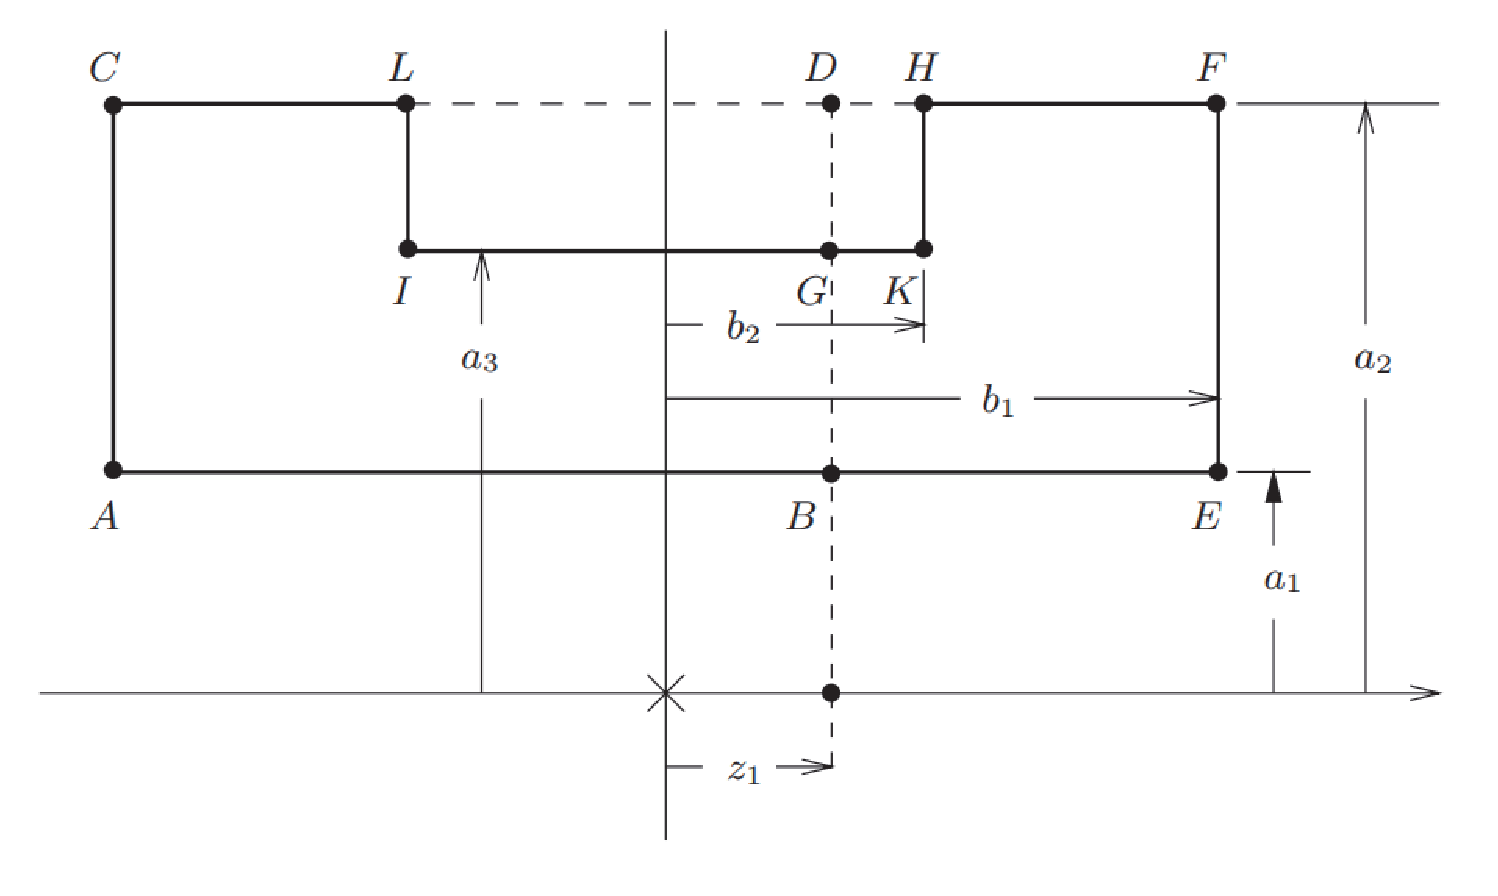
\includegraphics[scale=0.4]{chpt3/figs/fig3.27.eps}
	\caption{一个notched螺管的几何形状。}
\end{figure}


\subsubsection{问题3.7之解}
为了解出$H_z(0,z-1)$,我们可以把螺管分成四个单螺管,其截面参数按角点设计如下:

\textbf{螺管1}:ABDC,有$\alpha_1=a_2/a_1=\alpha,\beta_1=(b_1+z_1)/a_1=\beta+\gamma$,其中
$\beta=b_1/a_1,\gamma=z_1/a_1$;

\textbf{螺管2}:BEFD,有$\alpha_2=a_2/a_1=\alpha,\beta_2=(b_1-z_1)/a_1=\beta-\gamma$;

\textbf{螺管3}:IGDL,有$\alpha_3=a_2/a_3=\alpha^\prime,\beta_3=(b_2+z_1)/a_3=\beta^\prime+\gamma^\prime$,其中$\beta^\prime=b_2/a_3,\gamma^\prime=z_1/a_3$;

\textbf{螺管4}:GKHD,有$\alpha_4=a_2/a_3=\alpha^\prime,\beta_4=(b_2-z_1)/a_3=\beta^\prime-\gamma^\prime$;

注意到,所有螺管中,$J$都有相同的幅值,但螺管3和4与螺管1和2有相反的方向。同时注意到,所有的螺管都不是notched。

\textbf{螺管1的磁场}:$2_b=b_1+z_1$长的螺管1产生的$H_z(0, z_1)$是具有相同参数$a_1, a_2,\lambda J$而长度
为$2_b = 2(b_1+z_1)$的螺管产生的中心场的一半。
这从一个长为$2b$的非notched螺管的中心场$H_z(0, 0)$是两部分螺管产生的场(一部分从$z=−b$到$0$,另一部分
从$0$到$z=b$)之和这里看的更清楚。
也即,螺管的每一半产生总场$H_z(0, 0)$的一半。 于是:
\begin{equation}
H_{z}(0,z_{1})|_{1}=\frac{1}{2}\lambda Ja_{1}F(\alpha,\beta+\gamma)\\%(S7.1)
\end{equation}

\textbf{螺管2的磁场}:在$(0, z_1)$,$H_z$中来自长度$2_b = b_1−z_1$的螺管2的部分是具有相同$a_1, a_2,\lambda J$而长度为
$2_b = 2(b_1−z_1)$的螺管的中心场的一半。
\begin{equation}
H_{z}(0,z_{1})|_{2}=\frac{1}{2}\lambda Ja_{1}F(\alpha,\beta-\gamma)\\%(S7.2)
\end{equation}

\textbf{螺管3的磁场}:在$(0, z_1)$,$H_z$中来自长$2_b=b_2+z_1$的螺管3的部分四具有相同$a_3, a_2,\lambda J$
而长度为$2_b=2(b_2+z_1)$的螺管的中心场的一半。
因为$J$是反向的,我们有:
\begin{equation}
H_{Z}(0,z_{1})|_{3}=-\frac{1}{2}\lambda Ja_{3}F(\alpha',\beta'+\gamma')\\%(s7.3)
\end{equation}

\textbf{螺管4的磁场}:在$(0, z_1)$,$H_z$来自长$2_b = b_2−z_1$的螺管4的部分是除长为$2_b = 2(b_2−z_1)$而其他参数相同的螺管的中心场的一半。
\begin{equation}
H_{z}(0,z_{1})|_{4}=-\frac{1}{2}\lambda Ja_{3}F(\alpha',\beta'-\gamma')\\%(s7.4)
\end{equation}

\textbf{Notched螺管的磁场}

原notched螺管产生的$H_z(0,z_1)$于是可以由上四式之和给出:
\begin{equation}%3.127
\begin{split}
 H_{z}(0,z_{1}) =&H_{z}(0,z_{1})|_{1}+H_{z}(0,z_{1})|_{2}+H_{z}(0,z_{1})|_{3}+H_{z}(0,z_{1})|_{4} \\
=&\frac{1}{2}\lambda J a_{1}[F(\alpha,\beta+\gamma)+F(\alpha,\beta-\gamma)] \\%page115
&-\frac{1}{2}\lambda J a_{3}[F(\lambda',\beta'+\gamma')+F(\alpha',\beta'-\gamma')]
\end{split}
\end{equation}
\newpage


\subsection{讨论3.7:饼式线圈磁体的场分析}
应用讨论3.4中的叠加技术,我们推导可用于计算一个有2N个饼式线圈(N个双饼)组成的螺管磁体的场误差系数的轴向场表达式。
Bi2223和YBCO是带形式的,由高温超导带绕制的饼式线圈组成的磁体是实现空间高均匀度磁体(例如NMR和MRI磁体)
的一个可行途径[3.33, 3.34]。饼式线圈是薄的方截面导体的理想形式。

在这个分析中,每个饼都有相同的尺度——$2a_1;2a_2;2b=w$(带材宽度)——在饼线圈绕组中有相同的$\lambda J$。
相邻线圈分离距离为$\delta$。图3.28给出了一个由2N个单饼组成的磁体的剖面示意图。

在推导场方程时,所有的饼都对磁体原点居中。我们采用下面的简化记法。将$F(\alpha,\beta)/{\beta}$简记为:
\begin{equation}
\frac{F(\alpha,\beta)}{\beta}\equiv \ln(\alpha,\beta)=\ln\left[\frac{\alpha+\sqrt{\alpha^2+\beta^2}}{1+\sqrt{1+\beta^2}}\right]\\%(3.128)
\end{equation}

我们定义一个无量纲轴向磁场参数,$\eta(\zeta)\equiv H(z)/(\lambda J a_1)$,其中$\zeta\equiv z/a_1$。有:
\begin{equation}
\eta(\varsigma)\equiv \frac{H(Z)}{\lambda Ja_{1}}=\beta \ln(\alpha,\beta)\left[1+\sum_{j=1}^{n} E_{2j}(\alpha,\beta)\varsigma^{2j}\right]\\%(3.128b)
\end{equation}

因为使用了$\ln(\alpha,\beta)$,方程3.128b是一个无量纲场的表达式,与3.13a形式略有不同。
\begin{figure}[htbp]
	\centering
	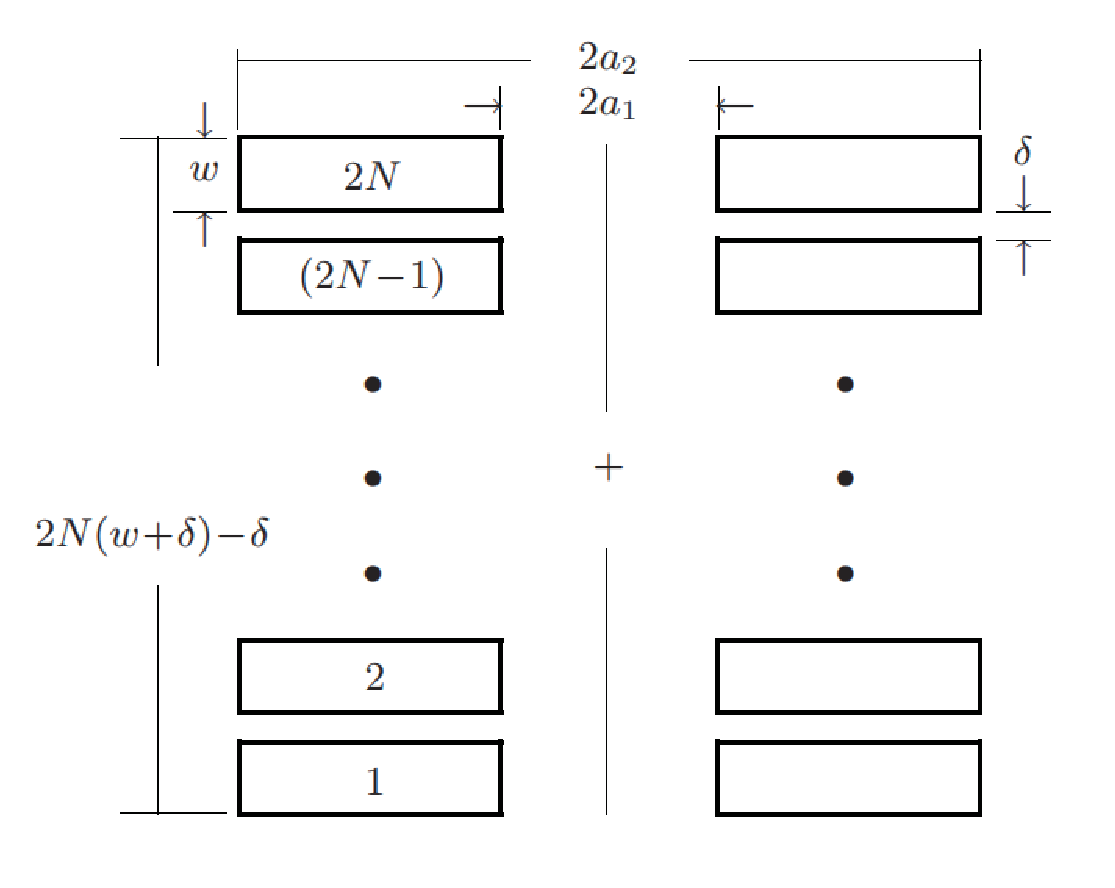
\includegraphics[scale=0.4]{chpt3/figs/fig3.28.eps}
	\caption{由2N个单饼(或N个双饼)组成的磁体}
\end{figure}

\begin{figure}[htbp]
	\centering
	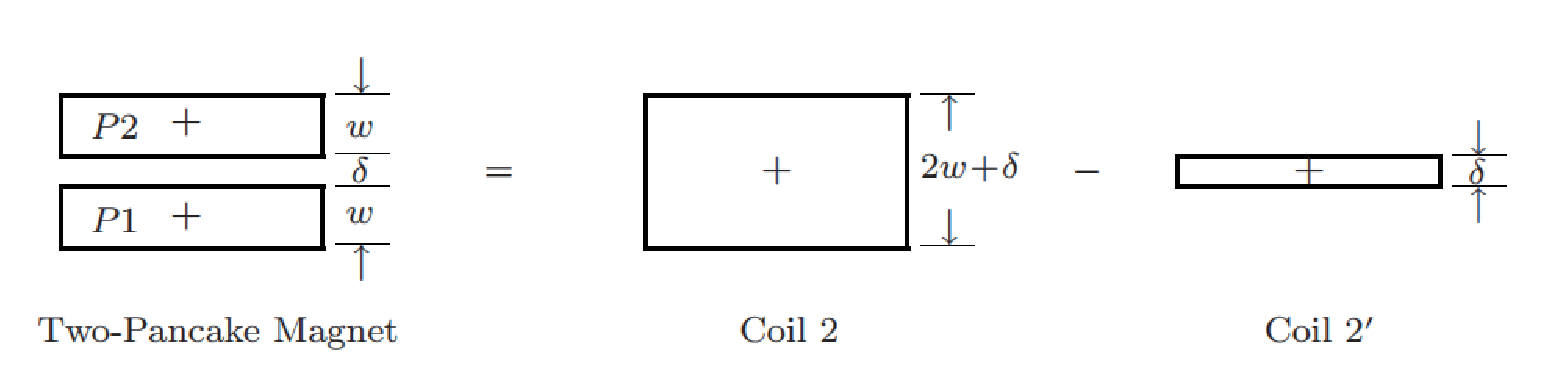
\includegraphics[scale=0.5]{chpt3/figs/fig3.29.eps}
	\caption{将双饼磁体视为线圈2减去线圈$2^\prime$,尺寸如图所注。}
\end{figure}

\textbf{第一步:二饼磁体——饼1和饼2}

首先考虑最简单的情况:一个由两个饼P1和P2组成的磁体。
采用讨论3.4中的叠加技术,原始具有间隙$\delta$(图3.29最左侧)的磁体与两个无间隙螺管等价:
高为$2b_2 = w +\delta$的线圈2(中部)减去高为$2b_2^\prime = \delta^\prime$的线圈$2^\prime$。
下标2为了标明考虑的磁体包括两个饼式线圈。
注意到图3.29中的每个线圈仅给出了高度($2b$),这是因为它是我们这个考虑下唯一相关的参数:
即线圈2有$\beta_2=(2w+\delta)/2a_1$;线圈$2^\prime$有$\beta_2=\delta/2a_1$。

与两个线圈有关的无量纲轴向场$\eta(\zeta)$为:
\begin{equation}
\eta_{2}(\varsigma)=[\eta(\varsigma)]_{2}-[\eta'(\varsigma)]_{2}\\%(3.129)
\end{equation}

从3.128b式,我们有:
\begin{eqnarray}
{[\eta(\varsigma)_{2}]}=\beta_{2}\ln(\alpha,\beta_{2})\left[1+\sum_{j=1}^{n}E_{2j}(\alpha,\beta_{2})\varsigma_{2j}\right]\\
{[\eta'(\varsigma)]}_{2}=\beta'_{2}\ln(\alpha,\beta'_{2}\left[1+\sum_{j=1}^{n}E_{2j}(\alpha,\beta'_{2})\varsigma^{2j}\right]%3.130b
\end{eqnarray}

组合3.129和3.130,我们有:
\begin{equation}
\begin{split}
\eta_{2}(\varsigma)=&[\beta_{2}\ln(\alpha,\beta_{2})-\beta'_{2}\ln(\alpha,\beta'_{2})]\\
&+\sum_{j=1}^{n}[\beta_{2}\ln(\alpha,\beta_{2})E_{2j}(\alpha,\beta_{2})-\beta'_{2}\ln(\alpha,\beta'_{2})]\varsigma^{2j}%(3.131)
\end{split}
\end{equation}

\textbf{第二步:四饼磁体——再加上饼3和饼4}

接下来,我们考虑一个由四个饼组成的磁体。
如图3.30所示,新磁体是第一步中的磁体上下各加一个磁体组成的。
这两个新的饼,如图3.30所给出的,可以建模为$2_b=4w+3\delta$的线圈4减去
$2_b=2w+3\delta$的线圈$4^\prime$。于是,线圈4有$\beta_4=(4w+3\delta)/2a_1$;
线圈$4^\prime$有$\beta_4^\prime=(2w+3\delta)/2a_1$。
\begin{figure}[htbp]
	\centering
	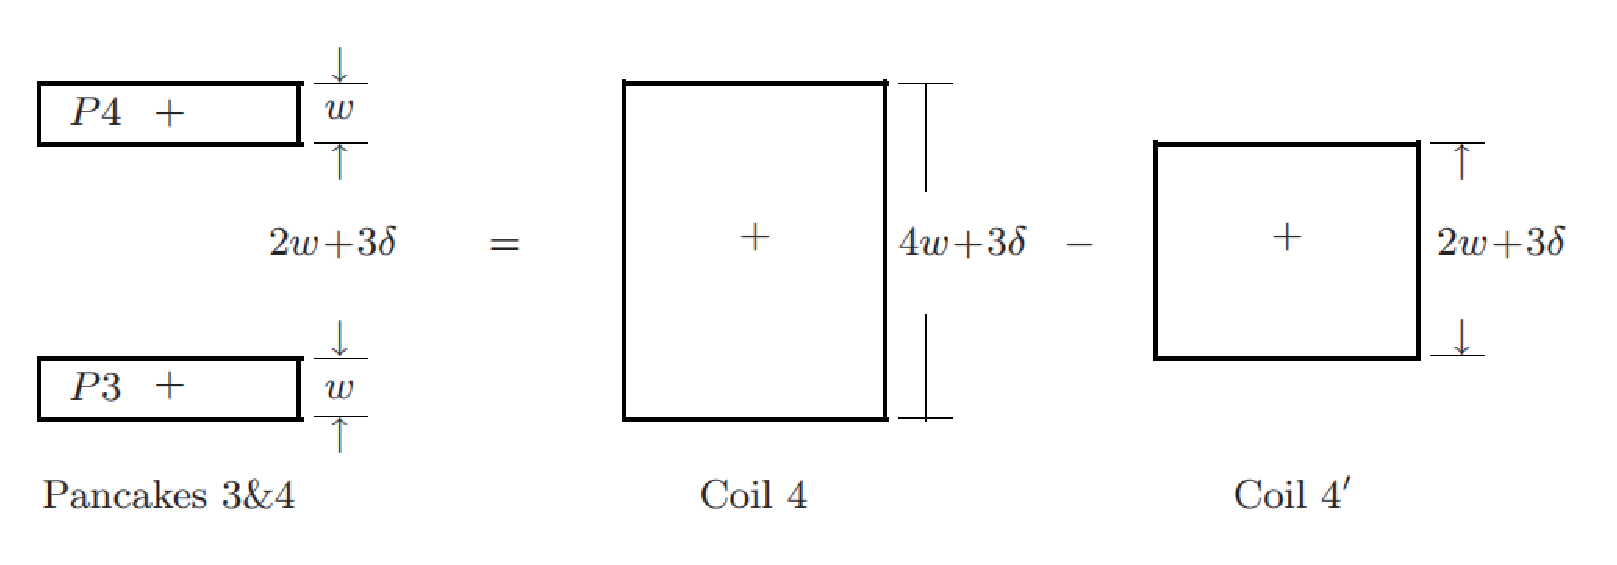
\includegraphics[scale=0.4]{chpt3/figs/fig3.30.eps}
	\caption{视为线圈4减去线圈$4^\prime$的磁体加入到图3.29的二饼磁体上组成的四饼磁体,尺寸如图所注。}
\end{figure}

来自所有四个线圈的总的无量纲轴向磁场$\eta_4(z)$为:
\begin{equation}
\eta_{4}(z)=[\eta(\varsigma)]_{2}-[\eta'(\varsigma)]_{2}+[\eta(\varsigma)]_{4}-[\eta'(z)]_{4}\\%(3.132)
\end{equation}

其中,
\begin{equation}
{[\eta(\varsigma)]}_{4}=\beta_{4}\ln(\alpha,\beta_{4})[1+\sum_{j=1}^{n}E_{2j}(\alpha,\beta_{4})\varsigma^{2j}]\\%(3.133a)
\end{equation}

\begin{equation}
{[\eta'(\varsigma)]}_{4}=\beta'_{4}\ln(\alpha,\beta'_{4})[1+\sum_{j=1}^{n}E_{2j}(\alpha,\beta'_{4})\varsigma^{2j}]\\%(3.133b)
\end{equation}

组合3.130和3.133,我们得到:
\begin{equation}
\begin{split}
\eta_{4}(\varsigma)=&[\beta_{2}\ln(\alpha,\beta_{2})+\beta_{4}\ln(\alpha,\beta_{4})]-[\beta'_{2}\ln(\alpha,\beta'_{2})+\beta'_{4}\ln(\alpha,\beta'_{4})]\\
&+\sum_{j=1}^{n}\{[\beta_{2}\ln(\alpha,\beta_{2})E_{2j}(\alpha,\beta_{2})+\beta_{4}\ln(\alpha,\beta_{4})E_{2j}(\alpha,\beta_{4})]\\
&-[\beta'_{2}\ln(\alpha,\beta'_{2})E_{2j}(\alpha,\beta'_{2})+\beta'_{4}\ln(\alpha,\beta'_{4})E_{2j}(\alpha,\beta'_{4})]\}\varsigma^{2j}%(3.134)
\end{split}
\end{equation}

\textbf{第三步:2N饼磁体——加上最后两个饼}

图3.31给出了2N饼磁体中最后两个饼$(2N−1)$和$2N$的模型。
线圈$2N$有$2b_N =2Nw+(2N−1)\delta$,由此$\beta_{2N}=[2Nw+(2N−1)\delta]/2a_1$;
线圈$2N^\prime$有$2b_N^\prime=2(N-1)w+(2N−1)\delta$,由此$\beta_{2N}^\prime=[2(N-1)w+(2N−1)\delta]/2a_1$。

由N个双饼组成的2N饼磁体的轴向磁场表达式:
\begin{equation}
\eta_{2N}(\varsigma)=\sum_{k=1}^{N}\{[\eta(\varsigma)]_{2k}-[\eta'(\varsigma)]_{2k}\}\\%(3.135)
\end{equation}

本分析中,我们假设双饼内部的间隙和相邻双饼之间的间隙是相等的。
\begin{figure}[htbp]
	\centering
	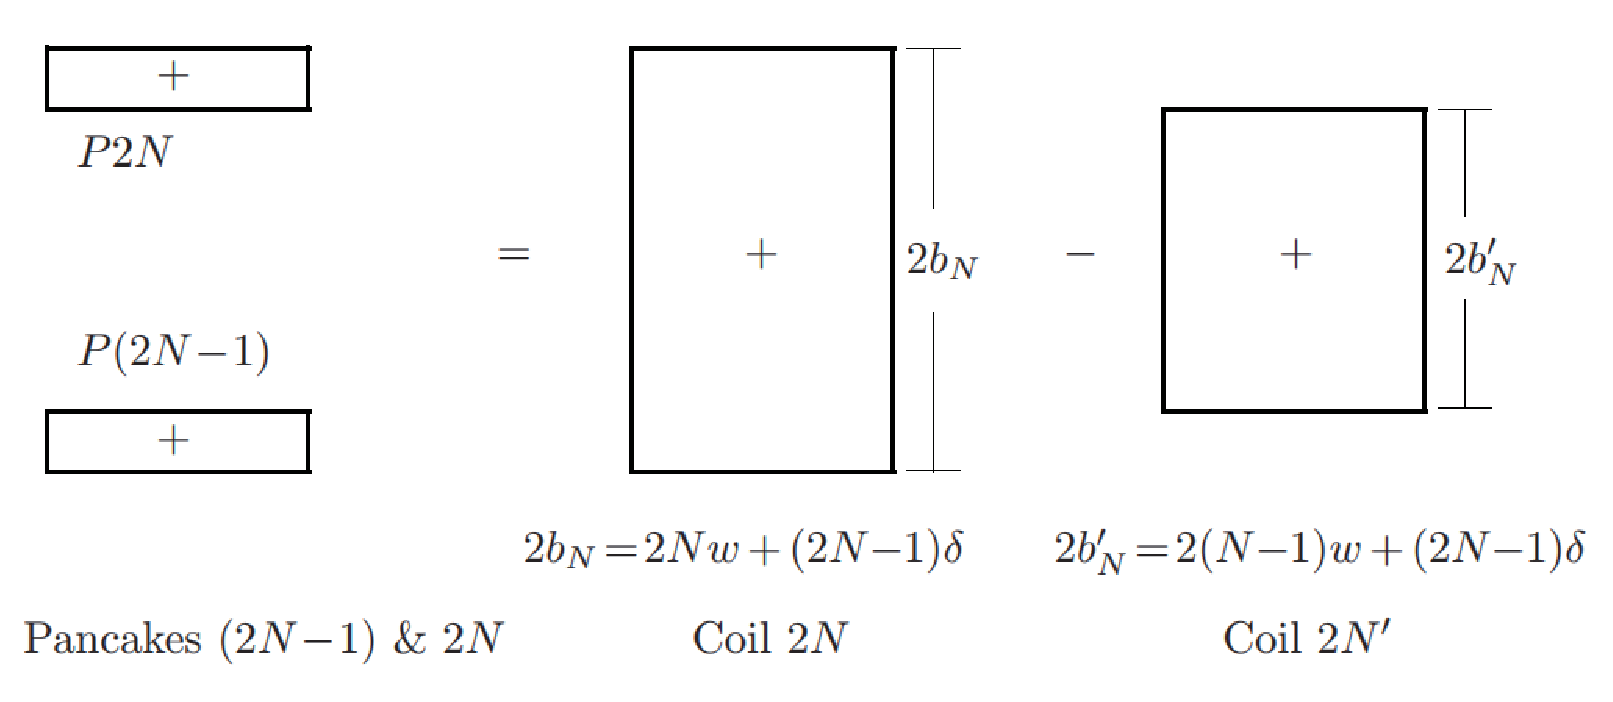
\includegraphics[scale=0.4]{chpt3/figs/fig3.31.eps}
	\caption{视为线圈2N减去线圈$2N^\prime$的磁体加入到$2(N-1)$饼式线圈磁体上。}
\end{figure}

我们可以将3.135用和3.134类似的形式表达:
\begin{equation}
\begin{split}
\eta_{2N}(\varsigma)=&\sum_{k=1}^{N}\{\left[\beta_{2k}ln(\alpha,\beta_{2k})-\beta'_{2k}ln(\alpha,\beta'_{2k})\right]\\
&+\sum_{j=1}^{n}[\beta_{2k}ln(\alpha,\beta_{2k})E_{2j}(\alpha,\beta_{2k})-\beta'_{2k}ln(\alpha,\beta'_{2k})E_{2j}(\alpha,\beta'_{2k})]\}\varsigma^{2j}%(3.136)
\end{split}
\end{equation}

式中,
\begin{equation}
\beta_{2k}=\frac{2k\omega+(sk-1)\delta}{2a_1}\\ \beta'_{2k}=\frac{2(k-1)\omega+(2k-1)\delta}{2a_{1}}\\
\end{equation}

式3.136也可以写作:
\begin{equation}
\frac{\eta_{2N}(\varsigma)}{\eta_{2N}(0)}=\{1+[E_{2}]_{2N}\varsigma^2+\cdots+[E_{2n}]_{2N}\varsigma^{2n}\}\\%(3.137)
\end{equation}

式中,$\eta_{2N}(0)$是无量纲中心场。$[E_{2n}]_{2N}$是第n阶总体误差系数。
$\eta_{2N}(\zeta=0)$和$[E_{2n}]_{2N}$为:
\begin{equation}
\eta_{2N}(0)=\sum_{k=1}^{N}[\beta_{2k}ln(\alpha,\beta_{2k})-\beta'_{2k}ln(\alpha,\beta'_{2k})]\\%3.138a)
\end{equation}

\begin{equation}
{[E_{2n}]}_{2N}=\frac{\sum_{k=1}^{N}[\beta_{2k}\ln(\alpha,\beta_{2k})E_{2n}(\alpha,\beta_{2k})-\beta'_{2k}\ln(\alpha,\beta'{2k})E_{2n}(\alpha,\beta'_{2k})]}{\sum_{k=1}^{N}[\beta_{2k}\ln(\alpha,\beta_{2k})-\beta'_{2k}\ln(\alpha,\beta'_{2k})]}\\%(3.138b)
\end{equation}

于是,方程3.138b给出了一个计算由2N个一致饼式线圈(各磁体有相同的$2a_1,2b=w,\alpha,\beta$,相邻间距$\delta$)组成的磁体第n阶误差系数的表达式。
\newpage


\subsection{问题3.8:理想双极磁体}
本问题研究理想双极磁体。此磁体无限长(从而无边缘效应)、绕组厚度为零、磁场由纵向表面电流产生、
磁场方向与双极磁体的轴垂直。
实际双极磁体的磁场和力的计算远比理想双极磁体复杂;
不过,除了在端部的复杂情况,理想双极磁体给出了双极磁体的大多关键特征。
双极磁体用于要求与磁体轴向垂直方向的磁场均匀的系统,例如高能粒子加速器[3.35–3.40]和发电机[3.41–3.43]。

一个半径为$R$、零绕组厚度的长(二维)双极磁体由双极壳($r=R$)上的$z$向的表面电流励磁。
室温孔内($r<R$)的磁场$\vec{H}_{d1}$以及壳外的磁场$\vec{H}_{d2}$为:
\begin{eqnarray}
\vec{H}_{d1}&=&H_{0}(sin\theta\vec{\imath}_{r}+cos\theta\vec{\imath}_{\theta})\\%3.139a)
\vec{H}_{d2}&=&H_{0}(\frac{R}{r})^2(sin\theta\vec{\imath}_{r}-cos\theta\vec{\imath}_{\theta})%(3.139b)
\end{eqnarray}

二维坐标的定义如图3.32。$+z$方向指向纸面外。在解答下面的问题时,忽略边缘效应。

a) 画出双极磁体$r<R$和$r>R$两个区域的场线。

b) 证明$r=R$处的表面电流的表达式为:
\begin{equation}
\vec{K}_{f}=-2H_{0}cos\theta\vec{\imath}_{z}\\%(3.140)
\end{equation}

画出方向草图,$\vec{K}_f$如果是$+z$方向,画圈(o);反之,画叉(×)。

c) 证明作用在载流壳单单元上的单位长度的Lorentz力密度表达式$\vec{f}_L$[$\mathrm{N/m^2}$]为:
\begin{equation}
\vec{f}_{L}=-\mu_{0}H_{0}^{2}sin2\theta\vec{\imath}_{\theta}\\%(3.141)
\end{equation}

\begin{figure}[htbp]
	\centering
	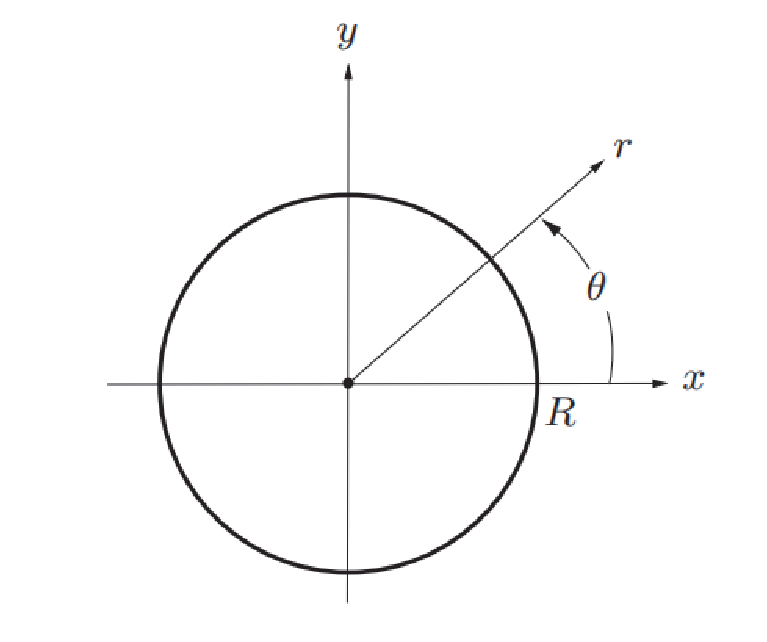
\includegraphics[scale=0.5]{chpt3/figs/fig3.32.eps}
	\caption{圆柱坐标系;$+z$朝向纸面外。}
\end{figure}

d) 证明施于右半部分($−90^\circ<\theta<90^\circ$)的净$x$向单位长度
Lorentz力$\vec{F}_{Lx}[\mathrm{N/m}]$为:
\begin{equation}
F_{Lx}=\frac{4R\mu_{0}H_{0}^{2}}{3}\\%(3.142)
\end{equation}

e) 证明单位长度储存的总磁能表达式$E_m[\mathrm{J/m}]$为:
\begin{equation}
E_{m}=\frac{\pi R^{2}B_{0}^{2}}{\mu_{0}}\\%(3.143)
\end{equation}

在$B_0=5\ \mathrm{T},R=20\ \mathrm{mm}$时计算$E_m$。
同时,由$E_m$计算一个长为$10\ \mathrm{m}$、载流$I_{op}=5000\ \mathrm{A}$的双极磁体的电感L。

为了减少双极磁体外部的磁场,在双极外装设一个厚度$d$的铁扼($\mu=\infty$),如图3.33所示。

f) 证明,在双极内部产生同样的磁场$\vec{H}$,需要的$\vec{K}_{f1}$恰为方程3.140的一半。
解释为什么电流减小了。

g) 实际中,铁扼不可能在无限的$H_0$下保持高$\mu$值。证明,为了保持铁扼不饱和,
最小的$d_m$表达式:
\begin{equation}
d_{m}=R(\frac{H_{0}}{M_{sa}})\\%(3.144)
\end{equation}

式中,$M_{sa}$是铁扼材料的饱和磁化。在以下条件下计算$d_m$:$\mu_0 H_0=5 T;\mu_0 M_{sa}=1.2\ \mathrm{T}; R=20\ \mathrm{mm}$。
\begin{figure}[htbp]
	\centering
	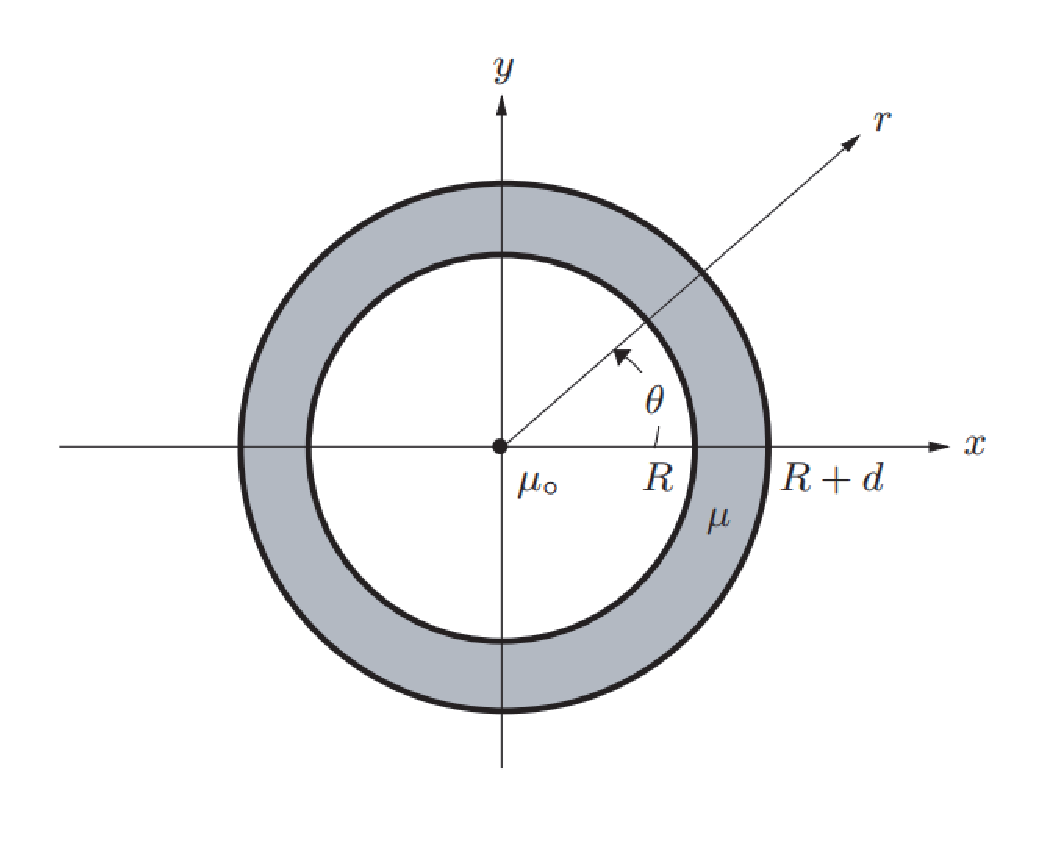
\includegraphics[scale=0.4]{chpt3/figs/fig3.33.eps}
	\caption{理想双极磁体外置厚度为$d$的铁扼}
\end{figure}

\subsubsection{问题3.8之解}
a) 场线示意图如图3.34a。磁场的法向($r$向)分量在边界处($r=R$)处是连续的。

b) 磁场的切向方向($\theta$向)在$r=R$处不连续,差值为该处的表面电流密度$\vec{K}_f$,
根据方程2.6,有:
\begin{equation}
\vec{K}_{f}=\vec{\imath}_{r}\times(\vec{H}_{d2}-\vec{H}_{d1})=\vec{\imath}_{r}\times-2H_{0}\cos\theta\vec{\imath}_{\theta}\\
=-2H_{0}\cos\theta\vec{\imath}_{z}\\%(3.140)
\end{equation}

如图3.34b指出的,$\vec{K}_f$在$-90^\circ<\theta<90^\circ$部分是指向$-z$向的,在
$90^\circ<\theta270^\circ$部分是指向$+z$向的。
\begin{figure}[htbp]
	\centering
	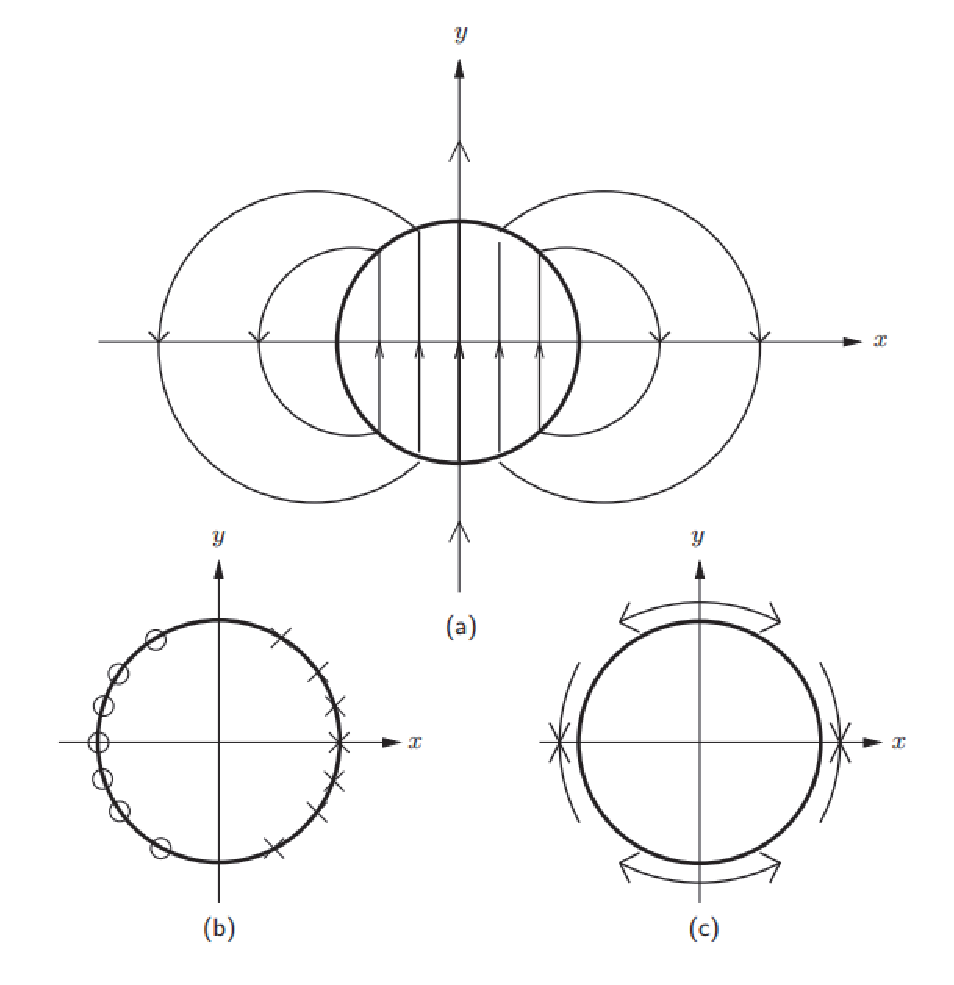
\includegraphics[scale=0.5]{chpt3/figs/fig3.34.eps}
	\caption{理想双极磁体。a) 内外场;b)表面电流密度矢量;c)力矢量。}
\end{figure}

c) $\vec{f}_L$由$\vec{K}_f\times\mu_0 \vec{H}_d$给出,其中$\mu_0 \vec{H}_d=\mu_0(\vec{H}_{d1}+\vec{H}_{d2})/2$:
\begin{eqnarray}
\vec{f}_{L}&=&\vec{K}_{f}\times\mu_{0}H_{0}\sin\theta\vec{\imath}_{r}%(S8.1)
=-2\mu_{0}H_{0}^{2}\cos\theta \sin\theta\vec{\imath}_{\theta}\\
&=&-\mu_{0}H_{0}^{2}\sin 2\theta\vec{\imath}_{\theta}%(3.141)
\end{eqnarray}

注意到,$\vec{f_L}$无$r$分量;它仅有$\theta$分量(图3.34c)。
同时,力密度在$\theta=\pi/4+n\pi/2$处最大,而在$\theta=0+n\pi/2$时为零,式中$n=0, 1, 2, 3$。
累计力$\propto\int f_L(\theta)d\theta$在$\theta=0$和$180^\circ$时取最大值。

d) 从图3.34c明显可见,施于右半部分的单位长度Lorentz力是$+x$方向的:
\begin{eqnarray}
F_{Ldx}&=&\int\vec{f}_{L}\cdot\vec{\imath}_{x}dx=-R\int_{\frac{-\pi}{2}}^{\frac{\pi}{2}}f_{L\theta}\sin\theta d\theta\\%(S8.2a)
&=&-2R\int_{0}^{\frac{\pi}{2}}f_{L\theta}\sin\theta d\theta=4R\mu_{0}H_{0}^{2}\int_{0}^{\frac{\pi}{2}}\cos\theta \sin^{2}\theta d\theta%(S8.2b)
\end{eqnarray}

从方程S8.2b,我们得:
\begin{equation}
F_{Lx}=\frac{4R\mu_{0}H_{0}^{2}}{3}%(3.142)
\end{equation}

施于左半部分的净Lorentz力和施于右半部分的Lorentz力的幅值相同,而指向$-x$向。
也就是说,存在一个很大的力试图将双极磁体的两部分拉开。
实际上,用于承受这个力的支撑结构的设计是双极磁体设计的关键点之一。

e) $E_m [J/m]$可以通过对磁能密度$\mu_0|H(r,\theta)|2/2$在垂直于双极轴的整个表面
(从$r=0$到$r=\infty$;从$\theta=0$到$\theta=2\pi$)积分获得。
\begin{eqnarray}
E_{m}&=&\frac{\mu_{0}}{2}\int_{0}^{R}|H_{d1}|^{2}2\pi rdr+\frac{\mu_{0}}{2}\int_{R}^{\infty}|H_{d2}|^{2}2\pi rdr\\%(S8.3a)
&=&\frac{\mu_{0}}{2}H_{0}^{2}\pi R^{2}+\frac{\mu_{0}}{2}H_{0}^{2}\pi R^{2}\\%(S8.3b)
&=&\mu_{0}\pi R^{2}H_{0}^{2}=\frac{\pi R^{2}B_{0}^{2}}{\mu_{0}}%(3.143)
\end{eqnarray}

从方程S8.3b可知,存储的总磁能可以分为双极壳内外的两个部分。
我们可以想象,双极内流动电流的一半用来产生$H_{d1}$而另一半用来产生$H_{d2}$。
代入$\mu_0 H_0=B_0=5\ \mathrm{T},R=20\ \mathrm{mm}$,有:
\begin{equation*}
E_{m}=\frac{\pi(2\times 10^{-2}m)^{2}(5T)^{2}}{4\pi\times10^{-7}H/m}=25kJ/m
\end{equation*}

对于一个5T双极磁体,如果长10 m,总存储磁能变为250 kJ。
总存储磁能等于双极磁体的总电感能。
\begin{equation}
\frac{1}{2}LI_{op}^{2}=250\ \mathrm{kJ}%(S8.4)
\end{equation}

代入$I_{op}=5000\ \mathrm{A}$解出L,有:
\begin{equation*}
L=\frac{2(250\times10^{3}\ \mathrm{J})}{(5000\ \mathrm{A})^{2}}=20\ \mathrm{mH}
\end{equation*}

在3.7.3节已给出,理想双极磁体单位长度的自感为: 
\begin{equation}
L_{\ell}=\frac{1}{8}\mu_{0}\pi N^{2}%(3.87)
\end{equation}

代入$L_{\ell}(=2\ \mathrm{mH/m})$以及$20\ \mathrm{mH}$,解出$N$,我们发现在$I_{op} = 5000\ \mathrm{A}$时$N\simeq 64$。
如果双极磁体的运行电流是$1000A$,那么磁体的电感必须是$0.5H$;它必须有5倍于$20\ \mathrm{mH}$双极
的绕组匝数: $N\simeq 318$。

f) 因为$\mu=\infty$,以及在$R< r< R+d$时$\vec{H}_{d2}=0$,如果屏蔽足够厚以避免饱和,
那么对$r>R+d$也有$\vec{H}_{d2}=0$。明显:
\begin{equation}
\vec{K}_{f1}=-H_{0}\cos\theta\vec{\imath}_{\theta}%(S8.5)
\end{equation}

这恰好是方程3.140中给出$\vec{K}_f$的一半。
考虑两种情况下都要求表面电流,我们可以作如下解释:全部用于产生室温孔场$-2H_0\cos\theta$的
表面电流,其中一半来自铁芯磁化的“表面电流”、

g) 单位长度的磁通$[Wb/m]$进入径向厚度为$d$的铁扼的0至$\theta=90^\circ$部分,必须等于或小于
$\mu_0 M_{sa}d$
\begin{equation}
R\mu_{0}H_{0}\int_{0}^{\frac{\pi}{2}}\sin\theta d\theta=R\mu_{0}H_{0}\leq\mu_{0}M_{sa}d%(S8.6)
\end{equation}

于是,铁扼的最小厚度为:
\begin{equation}
d_{m}=R(\frac{H_{0}}{M_{sa}})%(3.144)
\end{equation}

代入$R=20\ \mathrm{mm}, \mu_0 H_0=5\ \mathrm{T}, \mu_0 M_{sa}=1.2\ \mathrm{T}$,我们有:
\begin{equation*}
d_{m}=(20\ \mathrm{mm})\frac{5T}{1.2T}=83\ \mathrm{mm}
\end{equation*}

从表2.5可知,在$\mu_0 M=1.25\ \mathrm{T}$时,as-cast钢的磁导率为$180\mu_0$。尽管不是无限大,
但对于满足我们的无限大假设是足够用了。
\newpage

\subsection{问题3.9:理想四极磁体}
本问题研究一个理想四极磁体,该磁体无限长(无边缘效应)、零绕组厚度、纵向表面电流产生的磁场垂直于磁场轴线。
类似于双极磁体,四极磁体主要用于粒子加速器[3.35, 3.39, 3.44–3.46]。
如下文f)所论及的,四极磁体用于聚焦带电粒子束。

一个半径为$R$、零绕组厚度的“长”四极磁体由四极磁体壳体上($r=R$)沿$z$向流动的表面电流励磁。
室温孔内($r<R$)的磁场$\vec{H}_{q1}$和壳外($r>R$)的磁场$\vec{H}_{q2}$分别为:
\begin{eqnarray}
\vec{H}_{q1}&=&H_{0}\left(\frac{r}{R}\right)(\sin 2\theta\vec{\imath}+\cos 2\theta\vec{\imath}_{\theta})\\%(3.145a)
\vec{H}_{q2}&=&H_{0}\left(\frac{R}{r}\right)^{3}(\sin 2\theta\vec{\imath}_{r}-\cos 2\theta\vec{\imath}_{\theta})%(3.145b)
\end{eqnarray}

在解答下列问题时,忽略边缘效应。

a)画出四极磁体内外区域的场线。 

b)证明$r=R$处的表面电流$\vec{K}_f$表达式为:
\begin{equation}
\vec{K}_{f}=-2H_{0}\cos 2\theta\vec{\imath}_{z}%(3.146)
\end{equation}

大致画出电流的方向,在$\vec{K}_f$是$+z$向(指向纸面外)时画圈(o);反之,画叉(×)。

c)证明施加于壳体载流元上的单位长度Lorentz力密度的表达式为:
\begin{equation}
\vec{f}_{L}=-\mu_{0}H_{0}^{2}\sin 4\theta\vec{\imath}_{\theta}%(3.147)
\end{equation}

d)证明质子沿磁场中心以近乎光速$c$在$+z$向运动时,$x$向“磁弹性常数”$k_{Lx}$的表达式为:
\begin{equation}
k_{Lx}\simeq\frac{qc\mu_{0}H_{0}}{R}%(3.148)
\end{equation}

e)类似的,证明质子沿磁场中心以近乎光速$c$在$+z$向运动时,$y$向“磁弹性常数”$k_{Ly}$的表达式为:
\begin{equation}
k_{Ly}\simeq-\frac{qc\mu_{0}H_{0}}{R}%(3.149)\\
\end{equation}

f)通过阐明$k_{Lx}$和$k_{Ly}$是不稳定还是可恢复的,描述四极磁体在带电粒子加速器中的作用。

\subsubsection{问题3.9之解}
a)场线如图3.35a所示。对于理想情况,$r$分量在$r=R$处室连续的。

b)磁场的$\theta$分量在边界上的不连续等价于$r=R$处的表面电流密度,即:
\begin{equation}
\begin{split}
\vec{K}_{f}&=\vec{\imath}_{r}\times(\vec{H}_{q2}-\vec{H}_{q1})=\vec{\imath}_{r}\times-2H_{0}\cos 2\theta\vec{\imath}_{\theta}\\
&=-2H_{0}\cos 2\theta\vec{\imath}_{z}\\%(3.146)
\end{split}
\end{equation}

$\vec{K}_f$矢量在磁壳体上改变四次方向(图3.35b)。
\begin{figure}[htbp]
	\centering
	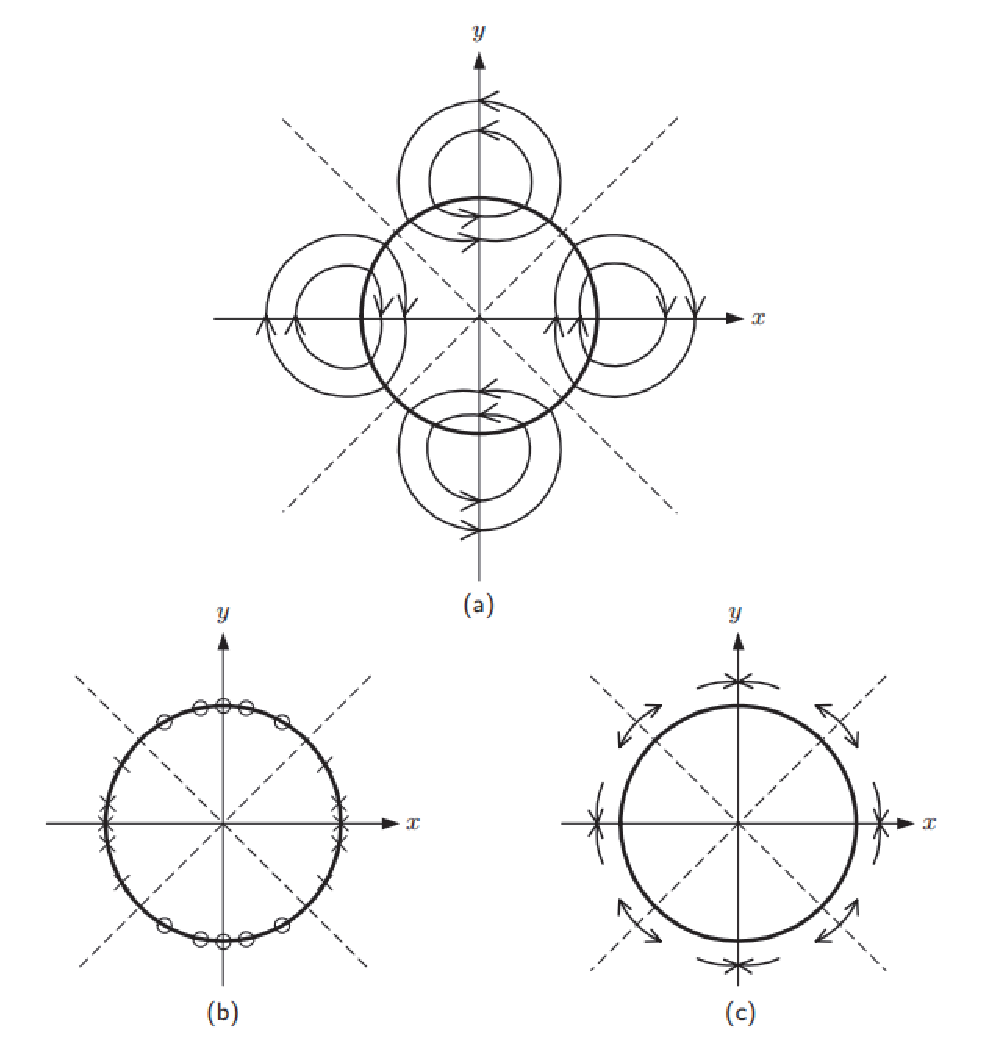
\includegraphics[scale=0.5]{chpt3/figs/fig3.35.eps}
	\caption{a) 四极磁体的内外磁场; b)磁体内的表面电流密度矢量; c) 磁体中力的方向。}
\end{figure}

c) $\vec{f}_L$由$r=R$处$\vec{K}_f$与$\mu_0 \vec{H}$的差积给出。
在$r=R$处,平均场$(\vec{H}_{q1}+\vec{H}_{q2})/2$就是$\vec{H}=H_0 \sin 2\theta\vec{\imath}_r$,因为
$\vec{H}_{q1}$的$r$分量与$\vec{H}_{q2}$的相抵消。注意到$\vec{K}_f=-2H_0 \cos 2\theta\vec{\imath}_\theta$,我们有:
\begin{equation}
\vec{f}_{L}=-2\mu_{0}H_{0}^{2}\sin 2\theta \cos 2\theta\vec{\imath}_{\theta}
=-\mu_{0}H_{0}^{2}\sin 4\theta\vec{\imath}_{\theta}%(3.147)
\end{equation}

$\vec{f}_L$的分布情况在图3.35c中画出。

d)我们可以将$x$方向的磁弹性系数定义为: 
\begin{equation}
k_{Lx}=-\frac{\partial F_{Lx}}{\partial x}%(S9.1)
\end{equation}

电荷为$q$的质子以近乎光速$c$在$z$向运动时,受到的$x$向Lorentz力密度$F_{Lx}$为:
\begin{equation}
F_{Lx}\simeq[q(c\vec{\imath}_{z})\times\mu_{0}H_{q1}\vec{\imath}_{\theta}]_{\theta=0}
\simeq-qc\mu_{0}H_{0}\left(\frac{r}{R}\right)\vec{\imath}_{x}%(S9.2)
\end{equation}

$k_{Lx}$于是由下式给出:
\begin{equation}
k_{Lx}=-\frac{\partial F_{Lx}}{\partial x}=-\frac{\partial F_{Lx}}{\partial r}
\simeq \frac{qc\mu_{0}H_{0}}{R}%(3.148)
\end{equation}

e) 在$y$向($r$向在$\theta=90^\circ$时),$F_{Ly}$为:
\begin{equation}
F_{Ly}\simeq[q(c\vec{\imath}_{z})\times\mu_{0}H_{q1}\vec{\imath}_{\theta}]_{\theta=\frac{\pi}{2}}
\simeq qc\mu_{0}H_{0}\left(\frac{r}{R}\right)\vec{\imath}_{y}\\%(S9.3)
\end{equation}

$k_{Ly}$于是由下式给出:
\begin{equation}
k_{Ly}=-\frac{\partial F_{Ly}}{\partial y}=-\frac{\partial F_{Ly}}{\partial r}
\simeq-\frac{qc \mu_{0}H_{0}}{R}\\%(3.149)
\end{equation}

f) $F_{Lx}$是恢复性的,但$F_{Ly}$是不稳定的,会令粒子束在$y$向发散。
在加速环中,四极磁体因此成对使用,一个用于在$x$向聚焦,紧跟另一个在$y$向聚焦;净效果是在两个方向都聚焦了。
\newpage



\subsection{讨论3.8:双跑道线圈磁体}
这里我们讨论一个由两个在磁体轴向正交平面方向相距$2c$的平行的长的\textbf{理想}“跑道”线圈。
跑道线圈的名字源导体末端绕过$180^\circ$,就像跑道一样。和双极磁体不同,它的绕组是平面的,即“平”的。
平的绕组让它相比于双极磁体更容易绕制,故而更适合用于发电机和电动机[3.47–3.50]。
跑道线圈同样也适合于磁悬浮[3.51–3.53]。

图3.36给出了由两个理想跑道线圈组成的磁体的绕组配置剖面图。
一组两个非常长的跑道线圈,彼此平行,某些情况下可以替代双极磁体。
例如,如果一天长超导带必须在一个横向于其主轴的均匀场下测试,就可以使用这种磁体;
它相较于双极磁体制作更容易。如图3.36给出的,每一个跑道线圈的绕组外宽度为$2a_2$,
内宽度为$2a_1$,有$N$匝。

右手侧的各跑道线圈的电流方向是$+z$向(指向纸外),左侧指向$-z$向。下面我们推导这种磁体的关键
参数表达式。
\begin{figure}[htbp]
	\centering
	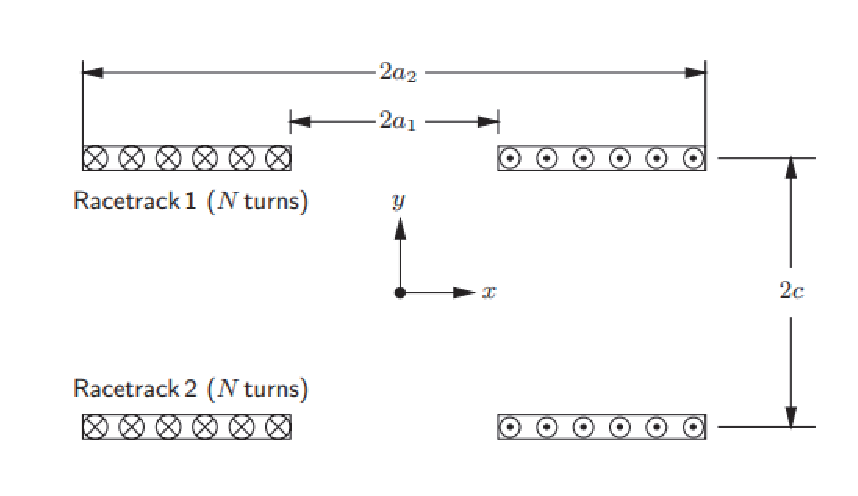
\includegraphics[scale=0.5]{chpt3/figs/fig3.36.eps}
	\caption{由两个理想跑道线圈组成的磁体剖面。}
\end{figure}

\textbf{A. 磁体中心场}

对右手侧跑道线圈1的$\xi$处的微分表面电流$Kd\xi$上应用Biot-Savart定律 (方程3.1),
我们会得到$(x,y)$处的微分磁场:
\begin{equation}
d\vec{H}_{1+}=\frac{K d\xi}{2\pi r_{1}}\vec{\imath}%(3.150)
\end{equation}

式中,磁场方向如图所示,$K=NI/(a_2-a_1)$。整个$+z$表面电流(从$\xi=a_1$到$\xi=a_2$)贡献的磁场的$y$分量$H_{y1+}$
可以通过从$\xi=a_1$到$\xi=a_2$对方程3.151积分得到:
\begin{equation}
H_{y1+}=-\frac{K}{2\pi}\int_{a_{1}}^{a_{2}}\frac{\cos\theta_{1}d\xi}{r_{1}}%(3.151)
\end{equation}

将$r_1=\sqrt{(\xi−x)^2+(c−y)^2}$和$\cos\theta_1=(\xi−x)/r_1$代入方程3.151,我们得到:
\begin{equation}
H_{y1+}=-\frac{K}{2\pi}\int_{a_{1}}^{a_{2}}\frac{(\xi-x)d\xi}{(\xi-x)^2+(c-y)^2}=
-\frac{K}{4\pi}\ln\left[\frac{(a_2-x)^2+(c-y)^2}{(a_1-x)^2+(c-y)^2}\right]%(3.152)
\end{equation}

类似的,其他电流的贡献:
\begin{eqnarray*}
% \nonumber % Remove numbering (before each equation)
H_{y1+}&=-\frac{K}{2\pi}\int_{a_{1}}^{a_{2}}\frac{(\xi-x)d\xi}{(\xi-x)^{2}+(c-y)^{2}}=-\frac{K}{4\pi}\ln\left[\frac{(a_{2}-x)^{2}+(c-y)^{2}}{(a_{1}-x)^{2}+(c-y)^{2}}\right]\\%(3.152a)
H_{y1-}&=-\frac{K}{2\pi}\int_{a_{1}}^{a_{2}}\frac{(\xi+x)d\xi}{(\xi+x)^{2}+(c-y)^{2}}=-\frac{K}{4\pi}\ln\left[\frac{(a_{2}+x)^{2}+(c-y)^{2}}{(a_{1}+x)^{2}+(c-y)^{2}}\right]\\%(3.152b)
H_{y2+}&=-\frac{K}{2\pi}\int_{a_{1}}^{a_{2}}\frac{(\xi-x)d\xi}{(\xi-x)^{2}+(c+y)^{2}}=-\frac{K}{4\pi}\ln\left[\frac{(a_{2}-x)^{2}+(c+y)^{2}}{(a_{1}-x)^{2}+(c+y)^{2}}\right]\\%(3.152c)
H_{y2-}&=-\frac{K}{2\pi}\int_{a_{1}}^{a_{2}}\frac{(\xi+x)d\xi}{(\xi+x)^{2}+(c+y)^{2}}=-\frac{K}{4\pi}\ln\left[\frac{(a_{2}+x)^{2}+(c+y)^{2}}{(a_{1}+x)^{2}+(c+y)^{2}}\right]%(3.152d)
\end{eqnarray*}

\begin{figure}[htbp]
	\centering
	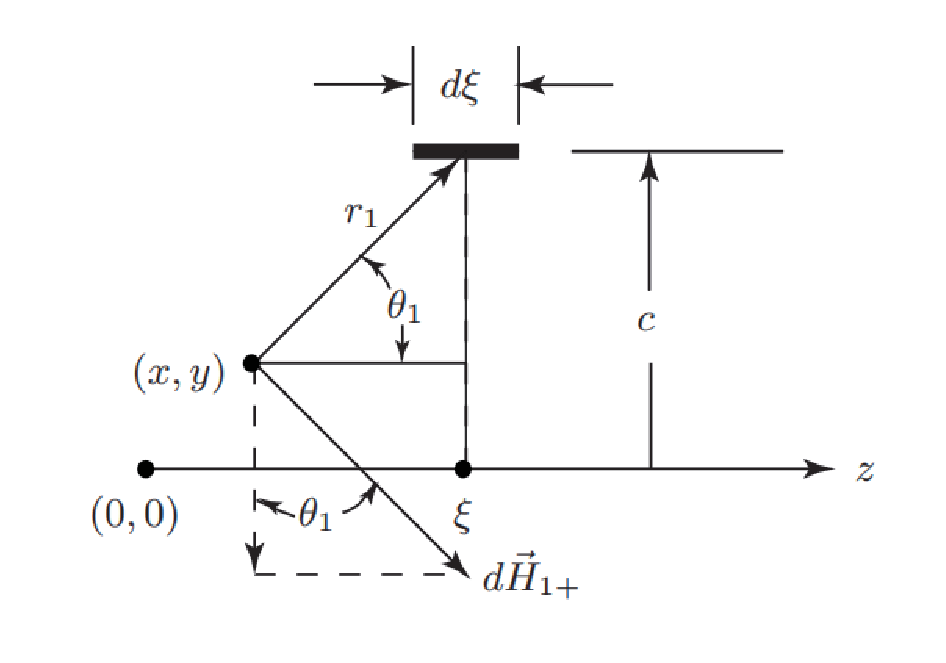
\includegraphics[scale=0.5]{chpt3/figs/fig3.37.eps}
	\caption{两个理想跑道线圈组成的磁体的剖面
	}
\end{figure}

组合上面四个贡献,有:
\begin{equation}
\begin{split}
H_{y}(x,y)=&-\frac{K}{\pi}\bigg\{\ln\left[\frac{(a_{2}-x)^{2}+(c-y)^{2}}{(a_{1}-x)+(c-y)^{2}}\right]+\ln\left[\frac{(a_{2}+x)^{2}+(c-y)^{2}}{(a_{1}+x)^{2}+(c-y)^{2}}\right]\\
&+\ln\left[\frac{(a_{2}-x)^{2}+(c+y)^{2}}{(a_{1}-x)^{2}+(c+y)^{2}}\right]+\ln\left[\frac{(a_{2}+x)^{2}+(c+y)^{2}}{(a_{1}+x)^{2}+(c+y)^{2}}\right]\bigg\}
\end{split}
\end{equation}


将$x=0$和$y=0$代入3.153a,有:
\begin{equation}
H_{y}(0,0)=-\frac{K}{\pi}\ln\left(\frac{a_{2}^{2}+c^{2}}{a_{1}^{2}+c^{2}}\right)%3.153b)
\end{equation}

\textbf{B. 中心附近的磁场}

我们可以通过求和$H_y(0,0)$与上面的导出的包含$H_{y1+}$的项来导出$H_y(x,y)$(方程3.153a)。
方程3.152a可以写为:
\begin{equation}
\begin{split}
H_{y1+}=&-\frac{K}{4\pi}\ln[\frac{(a_{2}-x)^{2}+(c-y)^{2}}{(a_{1}-x)^{2}+(c-y)^{2}}]\\
=&-\frac{K}{4\pi}\{\ln[(a_{2}-x)^{2}+(c-y)^{2}]-\ln[(a_{1}-x)^{2}+(c-y)^{2}]\}%(3.154)
\end{split}
\end{equation}

$\ln[(a2−x)^2+(c−y)^2]$可由下式给出:
\begin{equation*}
\begin{split}
\ln[(a_{2}-x)^{2}+(c-y)^{2}]=&\ln[(a_{2}^{2}+c^{2})(1+\frac{x^{2}+y^{2}-2a_{2}x-2cy}{a_{2}^{2}+c^{2}})]\\
=&\ln(a_{2}^{2}+c^{2})+\ln(1+\frac{x^{2}+y^{2}-2a_{2}x-2cy}{a_{2}^{2}+c^{2}})
\end{split}
\end{equation*}

在$|x|\ll 1$时,使用$\ln(1+x)\simeq x-x^2 /2$近似:
\begin{equation*}
\begin{split}
\ln[(a_{2}-x)^{2}+(c-y)^{2}]\simeq&\ln(a_{2}^{2}+c^{2})\\
&+\frac{(c^{2}-a_{2}^{2})(x^{2}-y^{2})-2(a_{2}^{2}+c^{2})(a_{2}x+cy)-4a_{2}cxy}{(a_{2}^{2}+c^{2})^{2}}
\end{split}
\end{equation*}

\begin{equation*}
\begin{split}
\ln[(a_{1}-x)^{2}+(c-y)^{2}]\simeq&\ln(a_{1}^{2}+c^{2})\\
&+\frac{(c^{2}-a_{1}^{2})(x^{2}-y^{2})-2(a_{1}^{2}+c^{2})(a_{1}x+cy)-4a_{1}cxy}{(a_{1}^{2}+c^{2})^{2}}
\end{split}
\end{equation*}

于是,方程3.154可以写为:
\begin{equation}
\begin{split}
H_{y1+}(x,y)\simeq&-\frac{K}{4\pi}[\ln(\frac{a_{2}^{2}+c^{2}}{a_{1}^{2}+c^{2}})+\frac{(c^{2}-a_{2}^{2})(x^{2}-y^{2})-2(a_{2}^{2}+c^{2})(a_{2}x+cy)-4a_{2}cxy}{(a_{2}^{2}+c^{2})^{2}}\\
&-\frac{(c^{2}-a_{1}^{2})(x^{2}-y^{2})-2(a_{1}^{2}+c^{2})(a_{1}x+cy)-4a_{1}cxy}{(a_{1}^{2}+c^{2})^{2}}]%(3.155a)
\end{split}
\end{equation}

类似的,$H_{y1−}, H_{y2+}, H_{y2−}$可以写成:
\begin{equation}
\begin{split}
H_{y2+}(x,y)\simeq&-\frac{K}{4\pi}[\ln(\frac{a_{2}^{2}+c^{2}}{a_{1}^{2}+c^{2}})+\frac{(c^{2}-a_{2}^{2})(x^{2}-y^{2})+2(a_{2}^{2}+c^{2})(a_{2}x+cy)-4a_{2}cxy}{(a_{2}^{2}+c^{2})^{2}}\\
&-\frac{(c^{2}-a_{1}^{2})(x^{2}-y^{2})+2(a_{1}^{2}+c^{2})(a_{1}x-cy)+4a_{1}cxy}{(a_{1}^{2}+c^{2})^{2}}]%(3.155b)
\end{split}
\end{equation}

\begin{equation}
\begin{split}
H_{y2+}(x,y)\simeq&-\frac{K}{4\pi}[\ln(\frac{a_{2}^{2}+c^{2}}{a_{1}^{2}+c^{2}})+\frac{(c^{2}-a_{2}^{2})(x^{2}-y^{2})-2(a_{2}^{2}+c^{2})(a_{2}x-cy)+4a_{2}cxy}{(a_{2}^{2}+c^{2})^{2}}\\
&-\frac{(c^{2}-a_{1}^{2})(x^{2}-y^{2})-2(a_{1}^{2}+c^{2})(a_{1}x-cy)+4a_{1}cxy}{(a_{1}^{2}+c6{2})^{2}}]%(3.155c)
\end{split}
\end{equation}

\begin{equation}
\begin{split}
H_{y2-}(x,y)\simeq&-\frac{K}{4\pi}[\ln(\frac{a_{2}^{2}+c^{2}}{a_{1}^{2}+c^{2}})+\frac{(c^{2}-a_{2}^{2})(x^{2}-y^{2})+2(a_{2}^{2}+c^{2})(a_{2}x+cy)-4a_{2}cxy}{(a_{2}^{2}+c^{2})^{2}}\\
&-\frac{(c^{2}-a_{1}^{2})(x^{2}-y^{2})+2(a_{1}^{2}+c^{2})(a_{1}x-cy)-4a_{1}cxy}{(a_{1}^{2}+c^{2})^{2}}]%3.155d)
\end{split}
\end{equation}

联立各项,在$(0,0)$附近,我们有:
\begin{equation}
\begin{split}
H_{y}(x,y)\simeq&-\frac{K}{\pi}[\ln(\frac{a_{2}^{2}+c^{2}}{a_{1}^{2}+c^{2}})-\frac{(a_{2}^{2}-a_{1}^{2})[3c^{4}+(a_{2}^{2}+a_{1}^{2})c^{2}-a_{2}^{2}a_{1}^{2}]}{(a_{2}^{2}+c^{2})^{2}(a_{1}^{2}+c^{2})^{2}}(x^{2}-y^{2})]\\
\simeq& H_{y}(0,0)+K[\frac{a_{2}^{2}-c^{2}}{(a_{2}^{2}+c^{2})^{2}}-\frac{a_{1}^{2}-c^{2}}{(a_{1}^{2}+c^{2})^{2}}](x^{2}-y^{2})\\%(3.156a)
\end{split}
\end{equation}

注意到,当$c^2$满足下式时,2阶不均匀项成为零:
\begin{equation}
\begin{split}
c^{2}=&\frac{1}{6}[\sqrt{(a_{2}^{2}+a_{1}^{2})^{2}+12a_{2}^{2}a_{1}^{2}}-(a_{2}^{2}+a_{1}^{2})]\\
=&\frac{1}{6}[\sqrt{a_{2}^{4}+14a_{2}^{2}a_{1}^{2}+a_{1}^{4}}-(a_{2}^{2}+a_{1}^{2})]%(3.156b)
\end{split}
\end{equation}

\textbf{C. 四个电流元素中心场}

我们通过近似将四个电流面视为载流为$NI$的载流元,可以进一步简化跑道线圈中心附近磁场的表达式,如
图3.38所示。点表示$+z$向,叉表示$-z$方向。

在这个案例中,我们令$a_1=a,a_2=a+\epsilon$以及$K\epsilon=K(a_2-a)=NI$。将这些参数代入方程3.153b中去。
考虑在$|x|\ll 1$时,有$\ln(1+x)=x$。于是:
\begin{equation}
\begin{split}
H_{y}(0,0)=&-\frac{K}{\pi}\ln(\frac{a_{2}^{2}+c^{2}}{a_{1}^{2}+c^{2}})\simeq-\frac{K}{\pi}\ln(\frac{a^{2}+c^{2}+2a\epsilon}{a^{2}+c^{2}})\\
\simeq&-\frac{K2a\epsilon}{\pi(a^{2}+c^{2})}\simeq-\frac{2aNI}{\pi(a^{2}+c^{2})}%(3.157a)
\end{split}
\end{equation}

\begin{figure}[htbp]
	\centering
	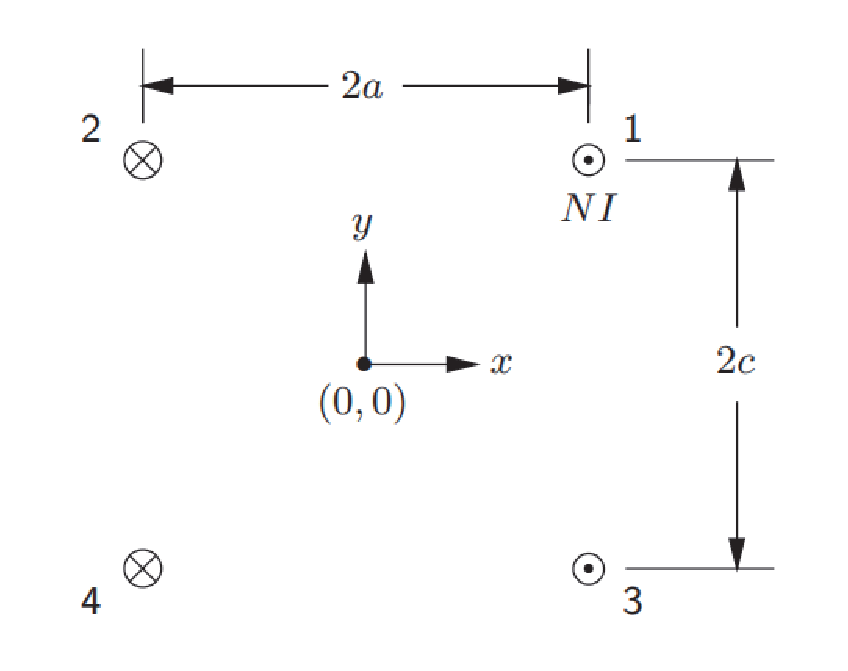
\includegraphics[scale=0.5]{chpt3/figs/fig3.38.eps}
	\caption{力计算用到的电流分布模型。}
\end{figure}

方程3.156a的等号右侧的第二项$K(a_2^2−a^2_1)=K(a_2+a_1)(a_2−a_1)$成为$2aNI$,于是:
\begin{equation*}
\begin{split}
\frac{K(a_{2}^{2}-a_{1}^{2})[3c^{4}+(a_{2}^{2}+a_{1}^{2})c^{2}-a_{c}^{2}a_{1}^{2}]}{\pi(a_{2}^{2}+c^{2})^{2}(a_{1}^{2}+c^{2})^{2}}(x^{2}-y^{2})\simeq&\frac{2aNI[3c^{4}+2a^{2}c^{2}-a_{4}]}{\pi(a^{2}+c^{2})^{4}}(x^{2}-y^{2})\\
=&-H_{y}(0,)[\frac{3c^{4}+2a^{2}c^{2}-a^{4}}{(a^{2}+c^{2})^{3}(x^{2}-y^{2})}]
\end{split}
\end{equation*}

联立上式和3.156,得到:
\begin{equation}
H_{y}(0,0)\simeq H_{h}(0,0)[1+\frac{3c^{4}+2a^{2}c^{2}-a^{4}}{(a^{2}+c^{2})^{3}}(x^{2}-y^{2})]%(3.157b)
\end{equation}

\textbf{D. 电流元上的力}

这四个相同的电流元模型可以用来计算施加于电流元1上的轴向单位长度的
Lorentz力$\vec{F_1}$。这个力是电流元2/3/4分别作用于电流元1上的Lorentz力之和:
\begin{equation}
\vec{F}_{1}=\vec{F}_{1}|_{2}+\vec{F}_{1}|_{3}+\vec{F}_{1}|_{4}%(3.158)
\end{equation}

式中,$\vec{F_1}|_2, \vec{F_1}|_3, \vec{F_1}|_4$分别是元素2/3/4作用在元素1上的力矢量。

载流为$I_2=NI$的元素2作用在载流为$I_1=NI$上的力$\vec{F_1}|_2$的方向为$+x$,为:
\begin{equation}
\vec{F}_{1}|_{2}=\frac{\mu_{0}I_{1}I_{2}}{4\pi a}\vec{\imath}_{x}=\frac{\mu_{0}N^{2}I^{2}}{4\pi a}\vec{\imath}_{x}%(3.159a)\\
\end{equation}

类似的,元素3在元素1上的力$\vec{F_1}|_3$是$-y$向的,为:
\begin{equation}
\vec{F}_{1}|_{3}=-\frac{\mu_{0}I_{1}I_{3}}{4\pi c}\vec{\imath_{y}}=-\frac{\mu_{0}N^{2}I^{2}}{4\pi c}\vec{\imath}_{y}%(3.159b)
\end{equation}

元素4对元素1的力$\vec{F_1}|_4$,既有$x$向,也有$y$向:
\begin{equation}
\begin{split}
\vec{F}_{1}|_{4}=&\frac{\mu_{0}I_{1}I_{4}}{4\pi\sqrt{a^{2}+c^{2}}}(\frac{a}{\sqrt{a^{2}+c^{2}}}\vec{\imath}_{x}+\frac{c}{\sqrt{a^{2}+c^{2}}}\vec{\imath}_{y})\\
=&\frac{\mu_{0}N^{2}I^{2}}{4\pi}(\frac{a}{a^{2}+c^{2}}\vec{\imath}_{x}+\frac{c}{a^{2}+c^{2}}\vec{\imath}_{y})%(3.159c)
\end{split}
\end{equation}

其他三个元素对元素1的电磁力的$x$分量和$y$分量$F_{1x}$和$F_{1y}$为:
\begin{eqnarray}
F_{1x}=&\frac{\mu_{0}N^{2}I^{2}}{4\pi}(\frac{1}{a}+\frac{a}{a^{2}+c^{2}})=\frac{\mu_{0}N^{2}I^{2}}{4\pi a}(1+\frac{a^{2}}{a^{2}+c^{2}})\\%(3.160a)
F_{1y}=&\frac{\mu_{0}N^{2}I^{2}}{4\pi}(-\frac{1}{c}+\frac{c}{a^{2}+c^{2}})=-\frac{\mu_{0}N^{2}I^{2}}{4\pi c}(1-\frac{c^{2}}{a^{2}+c^{2}})%(3.160b)
\end{eqnarray}

\textbf{E.跑道线圈自身内部以及两线圈之间的作用力}

因为$c^2 < a^2+c^2$,$F_{1y}$指向$-y$向。
跑道线圈1内部的元素1和元素2之间的净力是斥力,这是因为它们的电流极性相反。
类似的,跑道线圈2内部的元素3和4之间的净力也是斥力。
也即,如无外部约束,各跑道线圈都有扩展成圆形的趋势。

元素1和元素3之间的净力是引力,因为它们的电流极性是相同的。
类似的,元素2和元素4之间的净力也是引力。
如图3.160b所示,两个跑道线圈之间的净力是引力。
\newpage


\subsection{问题3.10:理想环状toroidal磁体}
本问题处理一个零绕组厚度的理想环形磁体,关键参数如图所示。

一个理想的圆截面环形磁体,大半径为$R$、小半径为$a$,由等效总安匝数$NI$的表面电流励磁
(图3.39)。假定表面电流围绕环流动,方向与$\phi$向垂直。

a) 证明环形磁体的内部磁场$B_\phi$为:
\begin{equation}
B_{\varphi}(r)=\frac{\mu_{0}NI}{2\pi r}%(3.161)
\end{equation}

同时证明,环外的磁场$B_\phi$是零。

b)假设环磁体已用有$N$个环,每个环载流均为$I$。证明,作用于单个环上的净径向洛伦兹力$F_{L+}$为:
\begin{equation}
F_{L+}=\frac{\mu_{0}NI^{2}}{2}(1-\frac{R}{\sqrt{R^{2}-a^{2}}})\\%(3.162)
\end{equation}
\begin{figure}[htbp]
	\centering
	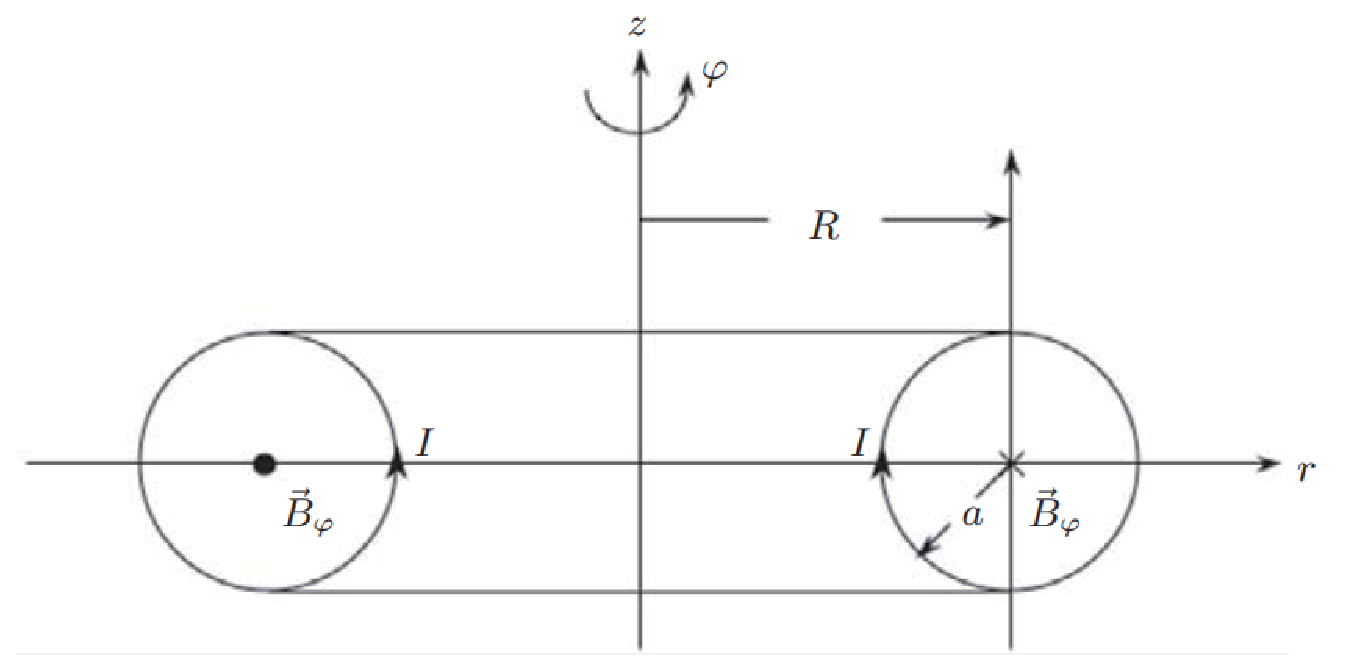
\includegraphics[scale=0.5]{chpt3/figs/fig3.39.eps}
	\caption{理想环形磁体,由N个环组成,每个环载流均为I。}
\end{figure}

\subsubsection{问题3.10之解}
a)根据对称性,我们看到$H_\phi$与$\phi$无关。在环形磁体内应用Ampere积分定律: 
\begin{equation}
\int_{0}^{2\pi}H_{\varphi}(r)rd\varphi=2\pi rH_{\varphi}(r)=NI%(S10.1)
\end{equation}

因为$B_\phi(r)=\mu_0 H_\phi(r)$,我们有:
\begin{equation}
B_{\varphi}(r)=\frac{\mu_{0}NI}{2\pi r}%(3.161)
\end{equation}

当上述积分在整个周长上进行时,环形磁体外部无净电流。故而,$H_\phi(r)=0,\ B_\phi(r)=0$。

b)图3.40给出了一个环,在它上面一个力微元$d\vec{F_L}$作用在一个微元$d\vec{s}$上。$r$方向的力微元为$dF_{Lr}$
$d\vec{F_L}$可以写为:
\begin{equation}
d\vec{F}_{L}=-Ids\vec{\imath}_{\theta}\times\tilde{B}_{\varphi}(r)\vec{\imath}_{\varphi}%(S10.2)
\end{equation}

式中,$\~{B}_{\phi}(r)$是作用在表面电流上的平均场。
这个场是方程3.161给出的场的一半。
\begin{equation}
d\vec{F}_{L}=-Ids\vec{\imath}_{\theta}\times\tilde{B}_{\varphi}(r)\vec{\imath}_{\varphi}=\frac{\mu_{0}NI^{2}ds}{4\pi r}\vec{\imath}_{\xi}%(S10.3)
\end{equation}

式中,$\vec{i_{\theta}}\xi$矢量与$\vec{F_L}$同向(Fig. 3.40)。该力微元的$r$分量写为:
\begin{equation}
dF_{Lr}=\frac{\mu_{0}NI^{2}\cos\theta ds}{4\pi r}\\%(10.4)
\end{equation}

\begin{figure}[htbp]
	\centering
	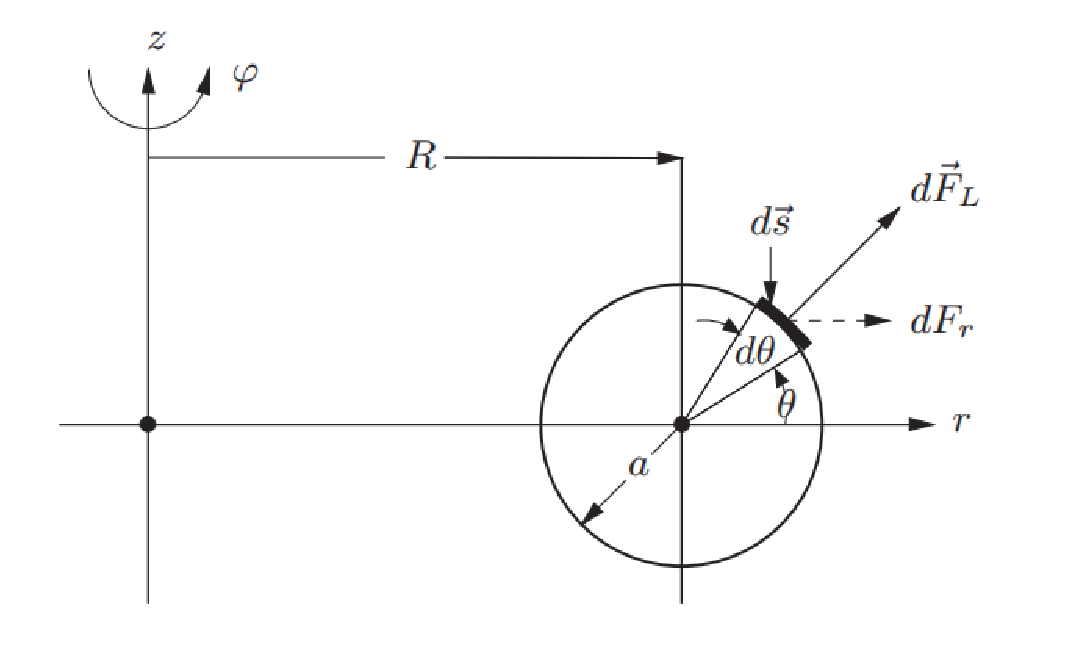
\includegraphics[scale=0.5]{chpt3/figs/fig3.40.eps}
	\caption{作用于单个环上的力微元。}
\end{figure}

因为$d s=a d\theta,r=R + a \cos\theta$,我们根据S10.4写出$dF_{Lr}$:
\begin{equation}
dF_{Lr}=\frac{\mu_{0}NI^{2}a\cos\theta d\theta}{4\pi(R+a\cos\theta)}%(S10.5)
\end{equation}

在整个小圆上对S10.5积分,有:
\begin{equation}
F_{Lr}=\frac{\mu_{0}NI^{2}a}{4\pi}\int_{0}^{2\pi}\frac{\cos\theta d\theta}{R+a\cos\theta}=\frac{\mu_{0}NI^{2}a}{2\pi}\int_{0}^{\pi}\frac{\cos\theta d\theta}{R+a\cos\theta}%(S10.6)
\end{equation}

查积分表,有:
\begin{equation}
\begin{split}
F_{Lx}=&\frac{\mu_{0}NI^{2}a}{2\pi}(\frac{\theta}{a}|_{0}^{\pi}-\frac{R}{a}\int_{0}^{\pi}\frac{d\theta}{R+a\cos\theta})\\
=&\frac{\mu_{0}NI^{2}a}{2\pi}\{\frac{\pi}{a}-\frac{2R}{a\sqrt{R^{2}-a^{2}}}\tan^{-1}[\sqrt{\frac{R-a}{R+a}}\tan\frac{\theta}{2}]_{0}^{\pi}\}%(S10.7a)
\end{split}
\end{equation}
\begin{equation}
F_{Lr}=\frac{\mu_{0}NI^{2}}{2}(1-\frac{R}{\sqrt{R^{2}-a^{2}}})%(3.162)
\end{equation}

当$R\rightarrow \infty$时,环形磁体成为直径为$2a$的直螺管。如我们所料,此时$F_{Lr}\rightarrow 0$。
\newpage


\subsection{讨论3.9:核聚变与磁约束}
如果轻元素核被约束并被加热到很高的温度($\sim 100\ \mathrm{MK}$),它们将发生聚变。
因为聚变产生的总质量$M_f$比原始核的总质量$M_n$要轻,反应会释放出静能量$E_n =(M_n−M_f)c^2$
,其中,$c$是光速。太阳通过这种过程产生能量。
一个可控的热核反应堆是一个小型的人造太阳。
太阳通过引力约束不稳定的热离子。
重力可以用磁体替代;使用磁场稳定热离子的技术称为磁约束。

聚变发电反应堆最可能使用一种采用磁约束的环形装置Tokamak。
Tokamak在1950年代由莫斯科kURchatov原子能研究所的L.A. Artsimovich和A.D. Sakharov提出。
国际热核实验反应堆(International Thermonuclear Experimental Reactor, ITER)项目
是一个联合欧盟、日本、俄罗斯、美国、韩国、中国和印度的合作项目。
ITER的目标是使用超导磁体制造一个现实可行的Tokamak。
ITER的环形磁体并未上面研究的圆截面,而是D型的,主半径$R\sim 8\ \mathrm{m}$,高约12 m;
它的环形磁场$B_\phi\sim 6 T$,
导体上的最大磁场约为13 T。ITER将在法国Cadarache完成制造。
\newpage


\subsection{问题3.11:边缘磁场}
本问题处理边缘磁场——磁体系统外部的不希望有的磁场。
边缘磁场很重要,因为它可能在磁体系统附近形成风险点;它还会对磁场敏感设备造成干扰或引起其失真。
为了计算远离磁场的边缘位置的磁场$vec{H_f}$,我们可以将磁体建模为一个有效半径为$R_e$的球形偶极子:
\begin{equation}
\vec{H}_{f}=H_{0}(\frac{R_{e}}{r})^{3}(cos\theta\vec{\imath}_{r}+\frac{1}{2}\sin\theta\vec{\imath}_{\theta})
\end{equation}
%(3.163)

式中,$\mu_0 H_0$是中心场。我们令方程3.163中给出的$z$轴($r$向,在$\theta=0$时)偶极远场($r\gg R$)等于
由方程3.3a给出的半径为$a$、载流为$I$的环($z\gg a$)。于是:
\begin{equation}
H_{0}R_{e}^{3}=\frac{1}{2}a^{2}I
\end{equation}

a)对一个安匝数为$NI$、内径$2a_1$、外径$2a_2$的螺管线圈,证明:采用加权平均$~{a}^2$,方程3.164修改为:
\begin{equation}
H_{0}R_{e}^{3}=\frac{1}{2}\tilde{a}^{2}NI=\frac{1}{6}(a_{1}^{2}+a_{2}^{2}+a_{1}a_{2})NI
\end{equation}

当方程3.164用于$n_{\ell}$组成的绕组的每一层时,每一层都有相同的匝数$n_{t/\ell}$。我们此处不加
推倒的给出一个表达式,请读者自行推导:
\begin{equation}
H_{0}R_{e}^{3}=\frac{1}{2}a_{1}^{2}NI[1+(\alpha-1)\frac{(n_{\ell}+1)}{n_{\ell}}+(\alpha-a)^{2}\frac{(n_{\ell}+1)(2n_{\ell}+1)}{6n_{\ell}^{2}}]
\end{equation}

注意到,$N=n_{t/\ell} n_{\ell}$。对于$n_{\ell}\gg1$,方程3.166可以由3.165近似。
因为$R_e$正比于各方程等号右侧的的立方根,多数情况下方程3.165是方程3.166的很好近似。
这些方程仅在$r\gg R_e$时有效,所以,方程3.165计算的$R_e$是无磁体长度$2b$和安匝数$NI$无关的。
对于由$k$个线圈嵌套组成的磁体,方程3.165可以推广为:
\begin{equation}
H_{0}R_{e}^{3}=\frac{1}{6}I\sum_{j=1}^{k}(a_{1j}^{2}+a_{2j}^{2}+a_{1j}a_{2j})N_{j}
\end{equation}

b) 使用方程3.167和表格3.3给出的参数,证明对45T超导磁体有$R_e=0.67 m $。 (因为
水冷磁体的体积比超导磁体的体积小很多,水冷磁体尽管其中心场为31T,但对边缘场仅贡献了一点点,可以忽略掉。)

c) 处于安全性考虑,与本磁体的运行和实验有关的人和设备必须位于磁体的100 gauss线外。
确定$z=2.75m$处的径向距离$r_m$,在此处边缘场幅值$|\mu_0 \vec{H_f}|$恰为100 gauss。

\subsubsection{问题3.11之解}
a)参数为$2a_1,2a_2$的螺管的加权平均$~{a}^2$可以写为:
\begin{equation}
\tilde{a}^{2}=\frac{1}{(a_{2}-a_{1})}\int_{a_{1}}^{a_{2}}r^{2}dr=\frac{(a_{2}^{3}-a_{1}^{3})}{3(a_{2}-a_{1})}=\frac{1}{3}(a_{1}^{2}+a_{2}^{2}+a_{1}a_{2})%(S11.1)
\end{equation}

于是:
\begin{equation}
H_{0}R_{e}^{3}=\frac{1}{2}\tilde{a}^{2}NI=\frac{1}{6}(a_{1}^{2}+a_{2}^{2}+a_{1}a_{2})NI\\%(3.165)
\end{equation}

b) 应用3.167和$H_0=14 T/\mu_0$到45T超导磁体 (表3.3) ,我们有:
%% 一个计算式
\begin{eqnarray}
\frac{14 T}{4\pi\times 10^{-7}H/m} R_e^3&= long numbers\\
(11.1408\times 10^6 A/m)R_E^3&=3.300\times 10^6 Am^2\\
R_e=0.667 m
\end{eqnarray}

c)在$I_{op}=10 kA$时,$\mu_0 \vec{H}_f=0.01 T (100 gauss)$,我们有:
\begin{eqnarray}
(0.01T)&=&(14T)(\frac{0.67m}{Rm})(\cos\theta\vec{\imath}_{r}+\frac{1}{2}\sin\theta\vec{\imath}_{\theta})\\
(R\ \mathrm{m})&=&\sqrt{(xm)^{2}+0+(2.7m)^{2}}\\%(S11.2b)
\theta&=&\tan^{-1}(\frac{xm}{2.7m})%(S11.2c)
\end{eqnarray}

在方程S11.2a, S11.2b和S11.2c中解出$x$,我们得到:$x=6.52 m$。
对于$x=6.52 m$,我们从方程S11.2b得到$R\simeq 7.05 m, \theta\simeq 67.5^\circ$。

注意到实验仪器在100 gauss磁场中暴露一天半天和在5 gauss中长期暴露是不同的。
\newpage


\subsection{讨论3.10:缩放一个螺管磁体}
在磁体设计的早期,缩放一个已经设计好的磁体的参数作为新磁体的参数有时候很方便并且也很快速。
缩放的时候通常的要求就是保持中心场$H_z(0,0)$或者功耗不变。
注意到下面的所有缩放定律尽管是针对螺管磁体提出的,但对任何形状的磁体都可以应用。

原始绕组尺寸$a_{1o}\equiv a_o;a_{2o}\equiv\alpha_o a_o;b_o\equiv \beta_o a_o$分别缩放$\chi$(>1为放大,<1为缩小)
得到一组新的绕组尺寸参数,其中的$\chi$是常数,
$a_{1\chi}=\chi a_o;a_{2\chi}=\chi\alpha_o a_o; b_\chi=\chi \beta_o a_o$。
下面的讨论中,所有的$o$下标参数都表原始磁体,$\chi$下标参数表示缩放后的新磁体。

我们感兴趣的参数包括:中心场$H_z(0, 0)\equiv H$;空间因数$\lambda$;总电流密度$J$;
运行电流$I$;导体截面积$A$;磁能$E$;总导体长度$\ell$;绕组体积$V$。
下面的讨论中,我们假设两个磁体的空间因数相同:$\lambda_\chi=\lambda_o=\lambda$。 

\textbf{A.空间均匀性}

如讨论3.4所述,螺管磁体的磁场的空间均匀性完全由$\alpha,\beta$确定。
因此,只要$\alpha,\beta$保持不变,全比例磁体将和原始磁体具有相同的均匀性。

\textbf{B.中心场 vs. 电流密度}

由方程3.13a(3.4和问题3.1),对于相同的$\lambda,\alpha,\beta$,中心场正比于$a_1 J$。
因为$a_{1\chi}=\chi a_o$,$J_\chi$必须缩放$1/\chi$:$J_\chi=J_O/\chi$。
因为磁压正比于$H_z^2(0, 0)$,所以新磁体的磁压与原磁体保持一致。
这从磁压正比于磁体的径向尺寸与运行电流密度的乘积$a_1 J$在缩放过程不变也能看出。
可以从方程3.54得到,新的磁体的中平面总的轴向力是原磁体的$\chi^2$——方程3.54中,$(NI/4b)^2$保持不变;
它是面积项,增长$\chi^2$。

\textbf{C.导体大小 \& 运行电流}

如果$I_\chi$缩放$\chi$,则缩放后的磁体的导体截面积$A_\chi\simeq I_\chi/J_\chi$要被缩放$\chi^2$:$A_\chi=\chi^2 A_o$。
另一方面,如果运行电流不变,那有$A_\chi=\chi A_o$。

\textbf{D. 总匝数}

缩放后磁体的总匝数,$N_\chi$,可以由下式给出:
\begin{equation}
N_{\chi}=\frac{\lambda J_{\chi}(2\beta a_{\chi})a_{\chi}(\alpha-1)}{I_{\chi}}%(3.168a)
\end{equation}

给定$A_\chi,J_\chi =J_o/\chi$,因为$H_z(0,0)$必须保持不变,$N_\chi$可保持不变或者必须按$\chi$缩放:
\begin{equation}
(for\ I_{\chi}=\chi I_{o})\quad N_{\chi}=\frac{\lambda(\frac{J_{o}}{\chi})(2\beta\chi a_{o})\chi a_{o}(a-1)}{\chi I_{o}}=N_{o}%(3.168b)
\end{equation}
\begin{equation}
(for\ I_{\chi}=I_{o})\quad  N_{\chi}=\frac{\lambda(\frac{J_{o}}{\chi})(2\beta\chi a_{o})\chi a_{o}(a-1)}{I_{o}}=\chi N_{o}%(3.168c)
\end{equation}

\textbf{E. 总导体长度、运行电流和安·米}

磁体所需的总导体长度,$\ell_\chi$,有两种选项:
\begin{equation}
(\mbox{对于}\ I_{\chi}=\chi I_{o})\quad \ell_{\chi}=N_{\chi} \pi (\alpha a_\chi+a_\chi)=N_{o}\chi \pi a_0(\alpha+1)=\chi \ell_{o}%(3.169a)
\end{equation}
\begin{equation}
(\mbox{对于}\ I_{\chi}=I_0)\quad \ell_{\chi}=\chi N_0 \chi \pi a_0 (\alpha+1)=\chi^2 \ell_{o}%(3.169b)
\end{equation}

总的安·米数,$I_\chi \ell_\chi$,是导体费用的一个很好的指标,在两种情况下都是按$\chi^2$缩放:
\begin{equation}
I_\chi \ell_\chi=\chi^2 I_0 \ell_0 %3.170
\end{equation}

\textbf{F. 总磁场能}

因磁体的总磁能是磁能密度在磁场所在的全部空间区域的积分,以及磁能密度不变,所以:
$E_{m\chi}=x^3E_{mo}$

\textbf{演示例子}

我们有一个如下参数的模型磁体:$H_z(0, 0) = 1.53\ \mathrm{T}; 2a_1 =
80\ \mathrm{mm}; 2a_2 = 130\ \mathrm{mm}; 2b = 220\ \mathrm{mm}$;总匝数$N_o = 2976$。
磁体自感$0.301\ \mathrm{H}$,在运行电流为$100\ \mathrm{A}$时产生的中心场为$1.53\ \mathrm{T}$。
下面我们考虑一个磁体,尺寸扩大10倍,空间因数保持不变。
我们计算几个新磁体的参数。

\textbf{自感}\ 因为$L_\chi=\mu_o a_\chi N_\chi^2L(\alpha,\beta)$,1)如果$I_\chi=\chi I$,$L_\chi=\chi L_o$;或者
2)如果$I_\chi=I_o$,$L_\chi=\chi^3L_o$。于是:1)如果$I_\chi=100\ \mathrm{A}$,有$L_\chi\simeq 3.01\ \mathrm{H}$;2)如果$I_\chi=10\ \mathrm{A}$,有$L_\chi\simeq 301\ \mathrm{H}$。

计算$\ell_o$:
\begin{equation}
\begin{split}
\ell_{o}=&N_{o}\frac{a_{o}(\alpha+1)}{2}\\
=&(2976)\frac{(0.04)(1.625+1)}{2}\simeq 156\ \mathrm{m}\\
\end{split}
\end{equation}

于是:1)如果$I_\chi=1000\ \mathrm{A}$,$\ell_{\chi}\simeq 1.56\ \mathrm{km}$;2)如果$I_\chi=100\ \mathrm{A}$,$\ell_{\chi}\simeq 15.6\ \mathrm{km}$。 
\newpage


\subsection{讨论3.11:粒子加速器}
电场($\vec{E}$)加速带电粒子的简单原理是粒子加速器的基础。
Cockroft-Walton (1928)和Van de Graaff (1930)的早期及其是线性的:沿一条直线以电势($\int\vec{E}\cdot\vec{s}$)加速粒子。
线性加速器需要很大的势能才能产生高能量粒子。因此,线性加速器需要大的电场$\vec{E}$或者长距离,
或两者兼有。斯坦福直线加速器($\sim 20 GeV$)的距离为2英里(3.2km)。

1930年代,Lawrence开发了一种圆形的回旋加速器。
现代圆形加速器是Lawrence斯回旋加速器的变种。
在圆形加速器中,带电粒子每次回旋时都以适度的电势加速;
通过多次回旋,可以将粒子加速到远远超过线性加速器可实现的能量水平。

圆形加速器的一个重要组件是一组用于产生磁场(通常为垂直方向)以使粒子沿圆周轨道运动的磁体。
现代加速器使用双极磁体,而Lawrence的首台$1.2\ \mathrm{MeV}$回旋加速器使用的是磁极片。

问题3.12将研究,圆形加速器中的粒子能量$E_p$正比于回旋半径$R_a$、粒子束速度和垂直磁场密度$B_z$。
CERN的强子对撞机(LHC)产生的最新的粒子能量为$7\ \mathrm{TeV}$,它意味着机器半径将近$3\ \mathrm{km}$!
作为对比,Lawrence的首台回旋加速器的半径是$\sim 0.1\ \mathrm{m}$。
如果LHC使用和Lawrence首台加速器一样的$\sim 1\ \mathrm{T}$的磁场$B_z$,那么半径需要增加
$\sim 3\times 10^4$仅能令$E_p$达到$\sim 0.8\ \mathrm{TeV}$。
在LHC中,通过增加磁场强度,扩大了$\sim 8$倍半径,实现了$7\ \mathrm{TeV}$。如此大的磁场,
仅超导双极磁体可以实现。
\newpage


\subsection{问题3.12:旋转加速器加速质子}
世界最大的对撞机LHC有$\sim 1250$个双极磁体,每一个都有$\sim 14 m$长,在直径$56 mm$的空间内产生$8.3T$的磁场。
LHC有两个相对运动的质子环束,每一部分被加速到$7 TeV$。

a) 椭圆形主环由两个半径为$R_a=2.8 km$的半圆组成,连接一个将近4.5km的直线部分。
双极磁体占满了两个半圆部分。
证明,双极磁场8.3T产生的Lorentz力$\vec{F_L}$平衡了$7 TeV$质子在圆部分的向心力$\vec{F_{cp}}$。
假设质子速度等于光速,$1 eV= 1.6\times 10^{−19} J$。

b)证明$7 TeV$的质子的速度接近光速。

\subsubsection{问题3.12之解}
a) 旋转质子的向心力 $\vec{F_{cp}}$被Lorentz力$\vec{F_L}$平衡。因为$F_{cp}$总是指向径向朝外的,所以需要
选择$B_z$的方向以保证$F_L$径向向心。两个力分别为:
\begin{equation}
\vec{F}_{cp}=\frac{M_{p}v^{2}}{R_{a}}\vec{\imath}_{r}\simeq\frac{M_{p}c^{2}}{Ra}\vec{\imath}_{r}=\frac{E_{p}}{R_{a}}\vec{\imath}_{r}\\%(S12.1a)
\end{equation}
\begin{equation}
\vec{F}_{L}=-qcB_{z}\vec{\imath}_{r}%(S12.1b)
\end{equation}

从$\vec{F}_{L}+\vec{F}_{cp}=0$中解出$R_a$,我们得到:
\begin{equation}
R_a=\frac{E_p}{q c B_z} %S12.2
\end{equation}

根据上式,我们有:
\begin{equation*}
R_{a}=\frac{(1.6\times 10^{-19}\frac{J}{eV})(7\times 10^{12}eV)}{(1.6\times 10^{-19}C)(3\times 10^{8}m/s)(8.3T)}\\
\simeq 2.81\times 10^{3}m\simeq 2.8 km
\end{equation*}

这笔LHC的实际半径(略超过4km)要小。
注意到上面的计算假定了整个环都被双极磁体占满;实际上,双极磁体的使用率是$\sim 60\%$——其余
部分空间被四极磁体、探测磁体占据。
沿着LHC环的平均双极场于是$\sim 5\ \mathrm{T}$,这样就会计算得到半径为$\sim 4\ \mathrm{km}$。
当然,双极场$B_z=15\ \mathrm{T}$将使环半径减半。$10-16\ \mathrm{T}$的超导双极磁体很容易造出来[3.54–3.56]。

b) 质子质量$M_p$,行进速度$v$与其静止速度有关:
\begin{equation}
M_{p}=\frac{M_{po}}{\sqrt{1-(\frac{v}{c})^{2}}}=\frac{E_{p}}{c^{2}}%(S12.3)
\end{equation}

在上式中解出$v/c$,有:
\begin{equation}
\frac{v}{c}=\sqrt{1-\frac{M_{po}^{2}c^{4}}{E_{p}^{2}}}\\%(S12.4)
\end{equation}

因为$v/c$非常接近1,方程S12.4可以近似为:
%%% 一个计算式
\begin{equation*}
\frac{v}{c}\simeq 1-\frac{M_po^2 c^4}{2E_p^2}\simeq 1-9\times 10^{-9}
\end{equation*}

可见,质子速度相当接近光速了。
\newpage



\subsection{问题3.13:两线圈磁体}
图3.41给出了一个由两个轴向对齐、完全相同的线圈A和B组成的磁体的剖面。两线圈的励磁极性相同。
轴向场$B_z$沿水平方向。如问题3.3指出的,反对称系统(Maxwell线圈)在中点($z=0$)产生线性的轴向场。
对称系统的线圈间的轴向作用力是引力;反对称系统配置下是大小相同的斥力。

两个绕组参数均为:$2a_1 = 1.5\ \mathrm{m}; 2a_2 = 2.1\ \mathrm{m}; 2b = 0.1\ \mathrm{m};
N =8900$和$I =65\ \mathrm{A}$。
左侧线圈轴中心位于$z=0.5 m$,右侧线圈位于$z = 0.5 m$——两线圈的中心距为$1 m$ (3.5节中的$\rho$)。
水平的黑色条代表两个线圈之间的室温结构支撑件。
图3.42a和3.42b分别给出了$B_z(r, z)$和$B_r(r, z)$在$I =65 A$的图。
注意,这里的$z=0$恰好与线圈轴向中点重合。
\begin{figure}[htbp]
	\centering
	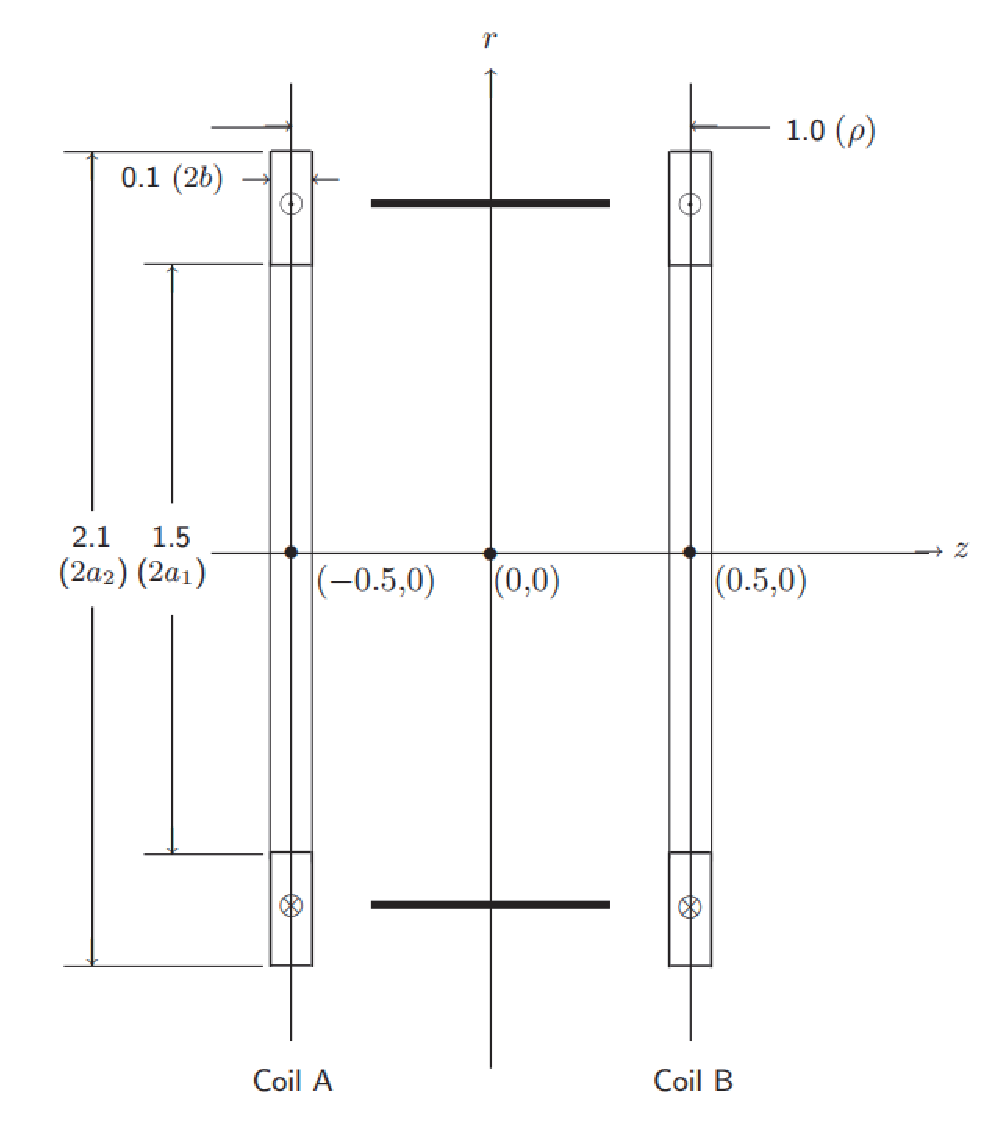
\includegraphics[scale=0.5]{chpt3/figs/fig3.41.eps}
	\caption{有两个相同线圈A和B在相同极性励磁下组成的磁体的剖面,尺寸以m为单位}
\end{figure}

\begin{figure}[htbp]
	\centering
	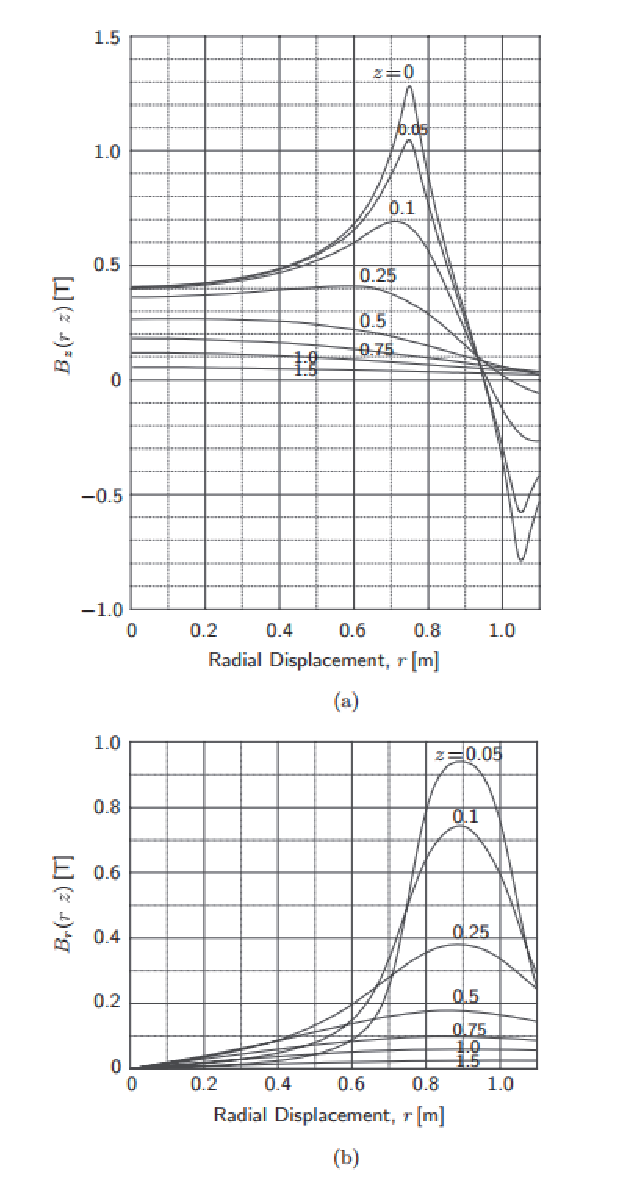
\includegraphics[scale=0.7]{chpt3/figs/fig3.42.eps}
	\caption{一个线圈未励磁,另一个线圈在$I=65A$时的(a)$B_z(r, z)$和(b) $B_r(r, z)$}
\end{figure}

a) 计算$I=65 A$时,线圈A的总体电流密度。

b) 计算线圈A绕组的总导体长度。

c) 使用恰当的解析表达,证明线圈A在$65A$、线圈B不励磁时的轴向中点处的$B_z$近似为0.4T,如图3.42a所示。

d) 使用图3.14中给出的螺管的$L(\alpha,\beta)$和方程3.81,计算线圈A的自感。某程序给出的数值是216.8 H。

f) 定量的证明,3.5.1中研究过的线圈A上的轴向力$F_{zA}(\rho)$在线圈B以$65A$励磁时是$+z$向的,即
线圈A和B之间的轴向力是引力。

g) 使用图3.42a和3.42b中合适的场数据,计算上述引力的幅值:两个线圈均以$65A$励磁。
结果应该在$2\times 10^5 N$的±20\%以内。(某程序计算值为−193 kN,负号表示引力。)

h) 将每个线圈近似为“环” (如图3.5),使用方程3.34计算线圈B施于线圈A上的轴向力$F_{zA}(\rho)$
使用$K(k) =2.10000,E(k)=1.2000,k=0.874157$。这里$a_A=a_B=0.9 m,\rho=1.0 m$。

i) 在$\rho=5 m$时计算$F_{zA}(\rho)$。

表3.6给出了这个两线圈系统的计算得到的互感 vs. 中心距数据,$M_{AB}(\rho)$。

j) 证明,系统存储的总能量$E_m$在运行电流$65A$、$\rho=1.0 m$时,近似为$1 MJ$。
使用$L=216.8 H$。

k) 在系统上应用方程3.105b,由$M_{AB}(\rho)$数据计算$F_{zA}(\rho)$。

\colorbox{red}{表3.6}

\subsubsection{问题3.13之解}
a)根据3.108a,有:
\begin{equation}
\lambda J=\frac{NI}{2b(a_{2}-a_{1})}\\%(3.108a)
=\frac{(4\pi\times 10^{-7}H/m)(8900)(65A)}{(1.5m)}(\frac{0.336}{0.4})=0.4T
\end{equation}

b) 导体总长度$\ell$为:$\ell=N\pi(a_2+a_1)\simeq 50.3 km$。于是这个两线圈系统的总导体长度
为$\sim 100\ \mathrm{km}$。

c) 我们可以将其中的一个线圈近似为$\alpha=1.4$的饼式线圈。通过应用3.111f,
我们得到线圈A的轴向中心场$B_{zA}$:
\begin{equation}
B_{zA}\simeq B_{z}(0,0)=\frac{\mu_{o}NI}{2a_{1}}(\frac{\ln\alpha}{\alpha-1})\\%(3.111f)
=\frac{(4\pi\times 10^{-7}H/m)(8900)(65A)}{(105m)}(\frac{0.336}{0.4})=0.4T
\end{equation}

d) 从图3.14,我们得到$L(\alpha=1.4, \beta=0.067)\simeq 2.8$。根据方程3.81,有:
\begin{equation}
L=\mu_{o}a_{1}N^{2}\mathcal{L}(\alpha,\beta)\\%(3.81)
=(4\pi\times 10^{-7}H/m)(0.75m)(8900)^{2}(2.8)=2.9H
\end{equation}

f)图3.42b中的$B_r(r, z)$在$z\ge 0$时成立,表明$B_r(r, z)$是正的,沿半径向外。
不过,当线圈B产生的$B_r(r, z)$施于线圈A时,因为线圈A相对于线圈B的轴向中点处于$z<0$,
线圈B施于线圈A的$B_r(r, z)$是沿半径向内的。如果对图3.41中的线圈A的顶部绕组截面应用
$I\vec{i_\theta}\times-B_r(r,z)\vec{i_r}$,线圈B施于线圈A的轴向力是$+z$向的,表明
这个力是引力。

g) $F_{zA}(\rho)$是Lorentz力,可由下式计算: 
\begin{equation}
F_{zA}(\rho)\simeq (average\ winding\ circumference)\times(NI)\times(B_r)=\pi(1.8)(8900\times 65)(0.06)=196\ \mathrm{kN}
\end{equation}

h)线圈B施于线圈A的力$F_{zA}(\rho)$为:
\begin{equation}
\begin{split}
F_{zA}(\rho)=&\frac{\mu_{o}}{2}(N_{A}I_{A})(N_{B}I_{B})\frac{\rho\sqrt{(a_{A}+a_{B})^{2}+\rho^{2}}}{(a_{A}-a_{B})^{2}+\rho^{2}}\\
&\times{k^{2}K(k)+(k^{2}-2)[K(k)-E(k)]}%(3.34)
\end{split}
\end{equation}

式中$K(k)$和$E(k)$分别是第一类和第二类完全椭圆积分:
\begin{equation*}
k^{2}=\frac{4a_{A}a_{B}}{(a_{A}+a_{B})^{2}+\rho^{2}}\\%(3.36)
\end{equation*}

这里,我们有$N_A=N_B=N =8900; a_A=a_B=(a_1+a_2)/2=0.9 m; \rho=1 m$:
%%公式
\begin{equation*}
k^2=\frac{4(0.9)(0.9)}{(0.9+0.9)^2+(1.0)^2}=0.764151\ \Rightarrow\ k=0.874157 
\end{equation*}

我们有$K(k)=2.100000$和$E(k)=1.200000$,于是:
\begin{equation*}
F_{zA}(1\ \mathrm{m})=long\ numbers\simeq -213.2\ \mathrm{kN}
\end{equation*}


i)在极限$ρ^2\gg(a_A+a_B)^2$下,方程3.34简化为:
\begin{equation}
F_{zA}(\rho)=\frac{3\mu_{o}}{2\pi}(\frac{\pi a_{A}^{2}N_{A}I_{A}}{\rho^{2}})(\frac{\pi a_{B}^{2}N_{B}I_{B}}{\rho^{2}})\\%(3.39c)
\end{equation}

$ρ^2=25.0 m^2$以及$(a_A+a_B)^2=3.24 m^2$,可知$ρ^2\gg(a_A+a_B)^2$是满足的。
因为$N_A=N_B=N =8900, I_A=I_B=65 A, a_A=b_B=0.9 m$,方程3.39c成为:
\begin{equation}
F_{zA}(\rho)=\frac{3(4\pi\times 10^{-7}\ \mathrm{H/m})}{2\pi}\left[\frac{\pi(0.9)^2(8900)(65)}{(5)^2}\right]^2=2.08\ \mathrm{kN}
\end{equation}

一个2 kN ($\sim 200$ kg)的力仅大约相当于单个线圈重量的13\%。

j)系统总磁能$E_m$可以由方程3.92给出:
\begin{equation}
E_{m}=\frac{1}{2}L_{1}I_{1}^{2}+\frac{1}{2}L_{2}I_{2}^{2}+M_{12}I_{1}I_{2}%(3.92)
\end{equation}

已知$L_1 = L_A = L_2 = L_B\equiv  L = 216.8 H, I_1 = I_A = I_2 = I_B\equiv I = 65 A$,从表中
可知$M_{AB}\simeq 29.8 H$,我们有:
%%公式
\begin{equation*}
	E_m=LI^2+M_{AB}I^2=(L+M_{AB})I^2=1.04\ \mathrm{MJ}
\end{equation*}

k)式3.105b如下给出:
\begin{equation}
F_{zR}(\rho)=\frac{\partial E_{AB}}{\partial \rho}=I_{A}I_{B}\frac{\partial M_{AB}(\rho)}{\partial\rho}\\%(3.105b)
\end{equation}

从表中可知,$M_{AB}(\rho=0.9 m)=34.873 H$以及$M_{AB}(\rho=1.1 m)=25.650 H$。于是:
\begin{equation}
\frac{\partial M_{AB}(\rho)}{\partial\rho}\simeq\frac{(25.650H-34.875H)}{(1.1m-0.9m)}=-46.115\ \mathrm{H/m}\\%(S17.1)
\end{equation}

将S17.1代入3.105b,并取$I_A=I_B=I =65 A$,有:
%%公式
\begin{equation*}
F_{zR}(\rho)\simeq (65)^2(-46.115)=-194.8\ \mathrm{kN}
\end{equation*}

毫不奇怪,这个数值和程序计算的−193 kN很接近。
\newpage

\subsection{问题3.14:螺管中平面上的轴向力}
本题我们使用3.5部分对$2a_1 = 10 cm; 2a_2 = 14 cm; 2b = 25 cm; NI = 1.5×10^6 A$(见图3.43a)的一个螺管中
推导出来的表达式。

a) 尽管这个螺管 ($\alpha = 1.4,\beta = 2.5$)实际上是既不“薄壁”也不“长”,
用方程3.111d计算$B_z(0, 0)$。

b) 将这个螺管视为“薄壁”,应用方程3.41a计算轴向中平面力$F_z(0)$。某程序计算结果是−187.8 kN。
使用$2a=10 cm$。

c) 使用对“长”螺管有效的方程3.41b,计算$F_z(0)$。选择螺管平均直径:1) $2a =10 cm$; 2) $2a=12 cm$。

d) 现在,将螺管分为两个子螺管A和B,如图3.43b所示。子线圈具有相同的半径1 cm,同时$2a_A=10 cm, 2a_B=12 cm,
NI =0.75\times10^6 A$。计算$B_z(0, 0)$。

e) 应用方程3.54计算,并与某程序的计算值$F_{zT}(0)=−187.8 kN$对比。

f) 应用对“长”螺管成立的方程3.55计算$F_{zT}(0)$。

g) 在“薄壁”且“长”的、有均匀表面电流密度$NI/2b$的螺管的一半的整个表面应用$\nabla\cdot B=0$。
需要考虑的表面是线圈的x-y平面上的$z=0$和$z=b$截面区域,分别为$\pi a^2$;以及在$r=a$时,从$z=0$
到$z=b$的圆柱表面区域,$2\pi ab$。

h) 对一个长螺管($\beta\gg 1$),解释为什么在它的长度方向从中平面到近末端的大部分区域的轴向力
是常数,并可由相应的中平面值给出。试着评估长螺管一半结构上$z$的位置,在该位置$B_z$开始
从$B_z(0,0)$显著下降。

表3.7给出了部分完全椭圆积分的值。
\begin{figure}[htbp]
	\centering
	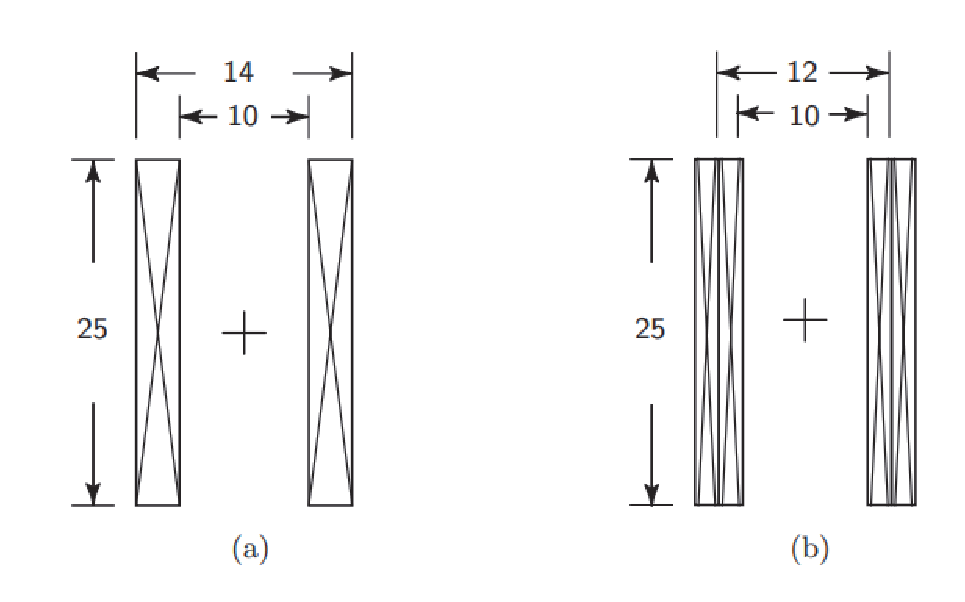
\includegraphics[scale=0.5]{chpt3/figs/fig3.43.eps}
	\caption{(a)参数为$2a_1=10cm; 2a_2=14cm; 2b=25cm$的螺管。
		(b)螺管分为两个子螺管A和B,参数为$2a_A=10cm; 2a_B=12cm; 2b=25cm$。}
\end{figure}
\textcolor{red}{表3.7}

\subsubsection{问题3.14之解}
a)应用3.111d,我们有:
\begin{equation}
B_{z}(0,0)=\frac{\mu_{o}NI}{2b}\\%(3.111d)
=\frac{(4\pi\times10^{-7}H/m)(1.5\times10^{6}A)}{(0.25m)}=7.5T\\
\end{equation}

方程3.109对这个$\alpha=1.4,\ \beta=2.5$的螺管给出的值时$B_z(0,0) = 6.8 T$。可知方程3.111d的误差
大约是10\%,考虑到它的简单性,这个结果不算太坏。

b)再次给出3.41a式:
\begin{equation}
F_{z}(0)=-\frac{\mu_{o}}{2}(\frac{NI}{2b})^{2}\{2b\sqrt{4a^{2}+b^{2}}[K(k_{b})-E(k_{b})]\\
-2b\sqrt{4a^{2}+4b^{2}}[K(k_{2b})-E(k_{2b})]\}\\%(3.41a)
\end{equation}

式中的模为:
\begin{eqnarray}
k_b^2=\frac{4a^2}{4a^2+b^2}=\frac{4(5)^2}{4(5)^2+(12.5)^2}\simeq 0.390244\\
k_{2b}^2=\frac{4a^2}{4a^2+(2b)^2}=\frac{4(5)^2}{4(5)^2+(25)^2}\simeq 0.137931
\end{eqnarray}

使用表3.7中给出的$K(k)$和$E(k)$合适值:
\begin{equation*}
F_z(0)= xxxxxxx \simeq -157.8\ \mathrm{kN}
\end{equation*}

上面这个值时某程序给出的值-187.8kN的84\%。

c)式3.41b如下给出:
\begin{equation}
F_{z}(0)\simeq-\frac{\mu_{o}}{2}(\frac{NI}{2b})^{2}\pi a^{2}\\%(3.41b)
\end{equation}

将$a=5 cm$和$a=6 cm$代入,有:
%%缺公式
\begin{eqnarray}
1)\qquad F_z(0)\simeq XXXXXX =-177.7\ \mathrm{kN}\\
2)\qquad F_z(0)\simeq YYYYYY = -255.8\ \mathrm{kN}
\end{eqnarray}

方程3.41b在$a=5 cm$时相比于程序值低估了大约5\%;在$a=6 cm$时高估了大约36\%。

d) 对每个子螺管应用方程2.111d;我们得到$B_z(0,0)$不变。
$$B_z(0,0) = B_{zA}(0,0) + B_{zB}(0,0)$$

e)再次给出式3.54:
\begin{equation}
\begin{split}
F_{zT}(0)=&-\frac{\mu_{o}}{2}(\frac{NI}{4b})^{2}\times\\
&(2b\sqrt{4a_{A}^{2}+b^{2}}[K(k_{bA})-E(k_{bA})]-2b\sqrt{4a_{A}^{2}+4b^{2}}[K(k_{2bA})-E(k_{2bA})]\\
&+2b\sqrt{4a_{B}^{2}+b^{2}}[K(k_{bB})-E(k_{bB})]-2b\sqrt{4a_{B}^{2}+4b^{2}}[K(k_{2bB})-E(k_{2bB})]\\
&-\frac{4b}{\sqrt{a_{T}^{2}+b^{2}}}\{(a_{T}^{2}+b^{2})[K(k_{b})-E(k_{b})]-\Upsilon(c^{2},k_{b})\}\\
&+\frac{4b}{\sqrt{a_{T}^{2}+4b^{2}}}\{(a_{T}^{2}+4b^{2})[K(k_{2b})-E(k_{2b})]-\Upsilon(c^{2},k_{2b})\})%(3.54)
\end{split}
\end{equation}

式中的$c^2$和其他模为:
\begin{eqnarray}
c^2&=&\frac{4a_A a_B}{(a_A+a_B)^2}\simeq 0.991736\\
k_{b_A}^2&=&\frac{4a_A^2}{4a_A^2+b^2}\simeq 0.390244\\
k_{2b_A}^2&=&\frac{4a_A^2}{4a_A^2+(2b)^2}\simeq 0.137931\\
k_{b_B}^2&=&\frac{4a_B^2}{4a_B^2+b^2}\simeq 0.479600\\
k_{2b_B}^2&=&\frac{4a_B^2}{4a_B^2+(2b)^2}\simeq 0.187256\\
k_{b}^2&=&\frac{4a_A a_B}{(a_A+a_B)^2+b^2}\simeq 0.432822\Rightarrow k_b\simeq 0.657892\\
k_{2b}^2&=&\frac{4a_A a_B}{(a_A+a_B)^2+(2b)^2}\simeq 0.160858\Rightarrow k_b\simeq 0.401071
\end{eqnarray}

将这些值和其他必要的值代入方程3.54,有:
\begin{equation}
F_z(0)= XXXXXX \simeq -168.9\ \mathrm{kN}
\end{equation}

计算值仍然相比程序值(−187.8 kN)有所低估,但是现在它是90\%。
尽管方程3.54给出的值相比3.41a要准确,但它相当繁琐,并不推荐用来作为快速估算力的方法。
很明显,将螺管分为两部分,应用方程3.54是口袋计算器手算的极限了。
方程3.41b在$a=5cm$时的良好结果更像是巧合,而不是一般规律。

f)在$a_A=5cm$和$a_B=6cm$时应用3.55,有:
\begin{equation}
F_z(0)\simeq XXXXXXX = -187.3\ \mathrm{kN}
\end{equation}

方程3.55相比于方程3.54更为简单,同样给出了至少对这个特殊的例子而言比3.54更好的结果。

g) 施加于$z\ge 0$部分所有匝上载流微元$dI$的力微元为:
\begin{equation*}
dF_z(z\ge 0)=-2\pi a B_r(z)d I
\end{equation*}

符号表示这个力是指向中平面的。做替换$dI = (NI/2b) dz$并在螺管的整个半区从$z=0$到$z=b$积分: 
\begin{equation}
F_{z}(0)=-\int_{0}^{b}2\pi aB_{r}(r)\frac{NI}{2}dz=-\frac{NI}{2b}\int_{0}^{b}2\pi aB_{r}(z)dz%(S14.1)
\end{equation}

积分$\int_0^b 2\pi a B_r(z)dz$是离开这半个螺管的总径向磁通。
根据$\nabla\cdot \vec{B}=0$,这等于从中平面($z=0$)圆面区域进入这一半螺管的总轴向磁通与在$z=b$处圆面区域离开
的磁通之差,也即:
\begin{equation}
\int_{0}^{b}2\pi aB_{r}(z)dz=\pi a^{2}[B_{z}(0)-B_{z}(b)]%(S14.2)
\end{equation}

方程3.41b的有效性是在假定螺管是“长”的($k^2\ll 1$或者$\beta\gg 1$)而得到的。
$B_z(0, 0),B_z(0, b)$可以假定在圆平面区域$\pi a^2$上保持不变。
对于长螺管,同时还有$B_z(0, b)\simeq 0.5 B_z(0,0)$(讨论3.4),于是S14.2可如下给出:
\begin{equation}
\int_{0}^{b}2\pi aB_{r}(z)dz\simeq\frac{\pi a^{2}}{2}B_{z}(0)\\%(S14.3)
\end{equation}

对长螺管,$B_z(0, 0)=\mu_0 NI/2b$ (方程3.111),于是:
\begin{equation}
\int_{0}^{b}2\pi aB_{r}(z)dz\simeq\frac{\pi a^{2}}{2}\times\frac{\mu_{o}NI}{2b}%%(S14.4)
\end{equation}

联立S14.1和S14.4,有:
\begin{equation}
F_{z}(0)\simeq-\frac{NI}{2b}\times\frac{\pi a^{2}}{2}\times\frac{\mu_{o}NI}{2b}\simeq-\frac{\mu_{o}}{2}(\frac{NI}{2B})^{2}\pi a^{2}%(3.41b)
\end{equation}

h) 对一个“长”螺管,$B_z(z)$不随$z$变化。$\nabla\cdot \vec{B}=0$要求径向分量$B_r(z)$总是零。
因为$F_z(z)$是由$B_r(z)$产生的(方程S14.1),$dF_z(z)=0$在线圈长度的大部分成立。
从而$F_z(z)$在$z=b$范围内保持常数,到了$z =b$,磁通线开始偏离磁场轴线,产生了$B_r(z)$,从而
产生$F_z(z)$。
对于$4b^2\gg 4a^2$和$(b+z)^2\gg 4a^2$,可以证明方程3.40中括号内的2阶和3阶线抵消了,仅剩一阶项,如下:
\begin{equation}
F_{z}(z\simeq b)\simeq-\frac{\mu_{o}}{2}(\frac{NI}{2b}^{2}\{(b-z)\sqrt{4a^{2}+(b-z)^{2}}[K(k_{b-})-E(k_{b-})]\}%(S14.5)
\end{equation}

因为$z$接近$b$,$k_{b−}^2 = 4a^2/[4a^2+(b−z)^2]$不满足$\ll 1$。于是,$K(k_{b−})−E(k_{b−})$不能由
$k_{b-}^2$近似。我们简单的猜想$z$在$b$附近的位置,此处$F_z(z\sim b)$与方程3.41b给出的近似。
如果我们猜$z=b-2a$,然后:
\begin{equation}
F_{z}(z=b-2a)\simeq-\frac{\mu_{o}}{2}(\frac{NI}{2b})^{2}\{2a\sqrt{4a^{2}+4a_{2}}[K(k_{b-})-E(k_{b-})]\}%(S14.6)
\end{equation}

式中,$k^2_{b-}=4a^2/8a^2 =0.5$,可由表3.1查到,$K(k_{b−} =0.7071)=1.8541,E(k_{b−})=1.3506$。
将这些值代入S14.6,有:
\begin{equation}
F_{z}(z=b-2a)\simeq-\frac{\mu_{o}}{2}(\frac{NI}{2b})^{2}4a^{2}\sqrt{2}(0.5035)\\
=-\frac{\mu_{o}}{2}(\frac{NI}{2b})^{2}2.85a^{2}%(S14.7)
\end{equation}

因为2.85大约是$\pi$的90\%,$F_z(z)$实际上是长螺管两端向内大约$2a$处的中平面力。
这个在长螺管轴向大部分区域的$F_z(z)$不变性也暗示了$B_z(z)$在轴向的同样长度区间内($2b-4a$)
差不多保持$B_z(0,0)$。
\newpage



\subsection{问题3.15:嵌套两线圈磁体的中平面上的力}
本问题中,我们计算由两个嵌套线圈组成的磁体中螺管A和螺管B的轴向压缩力,如图3.44所示。
两个螺管的轴向场都是指向$z$向的。
线圈参数如下:$2a_A=10\ \mathrm{cm};2b_A = 50\ \mathrm{cm}; N_A I_A = 3\times 10^6\ \mathrm{A};
2a_B = 14\ \mathrm{cm}; 2b_B = 100\ \mathrm{cm}; N_B I_B = 8\times10^6\ \mathrm{A}$。
各线圈的径向绕组厚度均为$1\ \mathrm{cm}$。

a) 视各螺管为“薄壁”($\alpha = 1$)和“长”($\beta\gg 1$),计算各线圈产生的中心场
$B_{zA}(0, 0)$和$B_{zB}(0, 0)$。证明,这个嵌套线圈磁体的中心场是$\sim 17.5\ \mathrm{T}$
(准确值为$17.31\ \mathrm{T}$)。

b) 使用方程3.57b,计算螺管A承受的总的中平面轴向力$F_{zA}(0)$。
某程序给出$F_{zA}(0)=-200.9\ \mathrm{kN}$。

c) 使用方程3.57a,再次计算$F_{zA}(0)$。
计算结果值应该比b)得到的更接近-200.9。

d) 使用方程3.59a,计算螺管B承受的总的中平面轴向力$F_{zB}(0)$。
某程序给出$F_{zB}(0)=-1207.5\ \mathrm{kN}$。

e) 解释为什么螺管A绕组内的最大场$B_{TA}=\sqrt{B_{zA}^2 + B_{rA}^2}$最可能
	出现在$r=a_A$和$z=0$。
	
f) 解释为什么螺管B绕组内的最大场$B_{TB}=\sqrt{B_{zB}^2 + B_{rB}^2}$不会出现,甚至也不会靠近$z=0$。
那它可能出现在什么位置呢?

表3.8给出了部分$\prod(c^2,k)$值。

\begin{figure}[htbp]
	\centering
	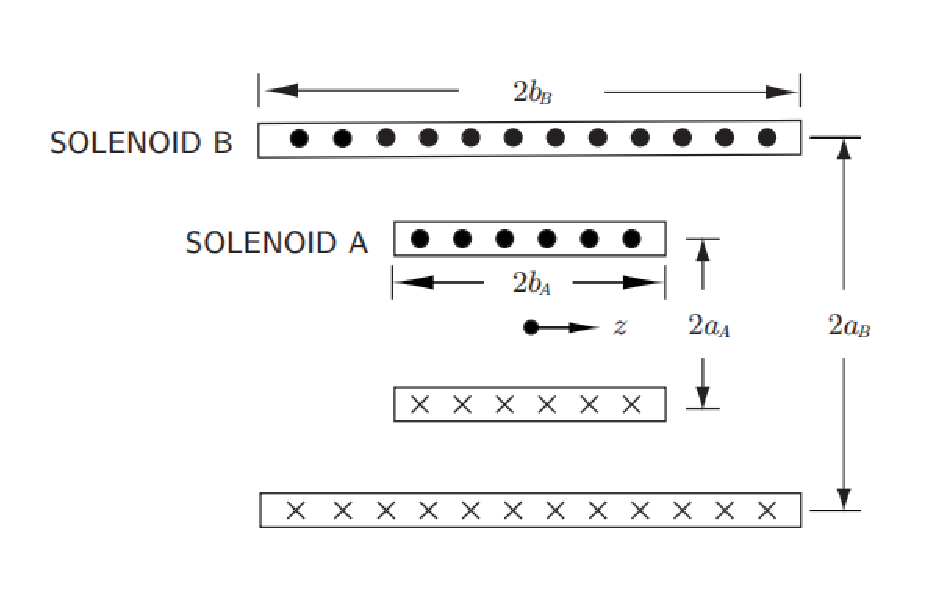
\includegraphics[scale=0.5]{chpt3/figs/fig3.44.eps}
	\caption{由两个“薄壁”($\alpha = 1$)线圈嵌套而成的两线圈磁体示意图。
		螺管A有$2a_A=10\ \mathrm{cm};2b_A = 50\ \mathrm{cm}$。
		螺管B有$2a_B = 14\ \mathrm{cm}; 2b_B = 100\ \mathrm{cm}$。}
\end{figure}
\colorbox{red}{表3.8}


\subsubsection{问题3.15之解}
a) 根据$B_z(0,0)=\mu_0H_z(0, 0)$以及方程3.111d,我们有:
\begin{eqnarray}
B_{zA}(0,0)=XXX\simeq 7.5\ \mathrm{T}\\
B_{zb}(0,0)=XXX\simeq 10.0\ \mathrm{T}\\
B_{z}(0,0)=XXX\simeq 17.5\ \mathrm{T}\\
\end{eqnarray}

如问题中给出的,准确的中心场值为17.32 T。

b) 式3.57b由下式给出:
\begin{equation}
F_{zA}(0)\simeq F_{zAA}(0)\simeq-\frac{\mu_{0}}{2}(\frac{N_{A}I_{A}}{2b_{A}})^{2}\pi a_{A}^{2}%(3.57b)
\end{equation}

代入合适的值,我们有:
\begin{equation}
F_{zA}\simeq -177.7\ \mathrm{kN}
\end{equation}

可见,方程3.57b的结果是程序计算值的88\%;两者的区别的部分原因是方程3.57b没有涵盖$F_{zAB}(0)$的贡献。 

c)式3.57a由下式给出:
\begin{equation}
\begin{split}
F_{zA}(0)\simeq&-\frac{\mu_{o}}{2}\{(\frac{N_{A}I_{A}}{2b_{A}})^{2}\pi a_{A}^{2}+(\frac{N_{B}I_{B}}{2b_{B}})(\frac{N_{A}I_{A}}{2b_{A}})\times\\
&(a_{A}-a_{B})^{2}[\Pi(c^{2},k_{D})+\Pi(c^{2},k_{r})-2\Pi(c^{2},k_{B})]\}\\(3.57a)
\end{split}
\end{equation}

式中,
\begin{eqnarray}
c^2= \\
k_B^2=\\
k_D^2=\\
k_T^2=
\end{eqnarray}

向方程3.57a中代入必要的值:
\begin{equation}
F_{zA}\simeq -183.7\ \mathrm{kN}
\end{equation}

这个值是 −200.9 kN的91\%;如我们所料,相对于b)有所提升,尽管不足以抵消增加的复杂性。 

d)式3.59a由下式给出:
\begin{equation}
\begin{split}
F_{zA}(0)\simeq&-\frac{\mu_{o}}{2}\{(\frac{N_{B}I_{B}}{2b_{B}})^{2}\pi a_{B}^{2}+(\frac{N_{B}I_{B}}{2b_{B}})(\frac{N_{A}I_{A}}{2b_{A}})[\pi(a_{A}^{2}+a_{B}^{2})\\
&-(a_{A}-a_{B})^{2}[2\prod(c^{2},k_{A})+\prod(c^{2},k_{D})-\prod(c^{2},k_{T})]]\}\\%(3.59a)
\end{split}
\end{equation}

式中,$c^2, k_D^2,k_T^2$已在上面给出;本例中,因为$b_A=b_D, k_A^2=k_D^2$,有:
\begin{equation}
F_{zB}\simeq -1063.4\ \mathrm{kN}
\end{equation}

这是程序值的88\%。

e) 因为$(2b_B)^2\gg (2b_A)^2$,在螺管A的室温孔内,螺管B产生的磁场和螺管A产生的磁场都是均匀的且仅有轴向。
所以,螺管A内部的最大场,大约17.5 T,出现在$z=0$处的最内侧半径上。
根据同一个程序的计算结果,最大场17.32 T出现在($r=5 cm,z=0$)。

f) 再次,因为$(2b_B)^2\gg (2b_A)^2$,the radial field component of Solenoid A impinges on Solenoid B away from its center point where the axial field of Solenoid B is still essentially the same as that at its midplane. 因此,很可能螺管B的最大场可能超过10.0 T,螺管B的中平面场(程序给出为9.94 T),出现在轴向距离中心$\sim \pm b_A$的地方。
程序给出的螺管B中的最大场是9.96 T ($B_r = \pm 1.70 T;B_z =9.81 T$),出现在($r=7 cm, z=\pm 25 cm$)。注意,
$b_A=25 cm$。
\newpage


\subsection{问题3.16:环氧浸渍螺管的应力}
本例简单的近似处理环氧浸渍磁体的应力计算。
我们使用一个FBNML制造于1970年代的500-MHz (12 T) NMR超导磁体作为实例[3.57]。
该磁体有一个高场内插磁体,一个主线圈和多个矫正补偿线圈。
主磁体绕组的内半径$a_1$为72.6 mm,绕组的外半径($a_2$)为102 mm,绕组长度($2b$)是488 mm。
主线圈由Nb-Ti导体绕成;铜和NiTi的体积比是2.1。
这种复合导线的直径是裸线0.63 mm ($D_{cd}$),绝缘后0.71 mm($D_{ov}$)。
绕组是紧凑的六边形配置。导线之间的间隙填充了环氧树脂。
图3.45给出了该配置下的三条相邻导线。

当所有线圈都励磁后,磁场$B_z$的轴向($z$)分量在主线圈范围内随径向距离$r$线性减小。
在主线圈的中平面($z = 0$)上,当$r = a_1$时$B_z=8.22T$,当$r = a_2$时$B_z=-0.21T$。
$B_z$的线性降低在$z=0$是相当准确。
主线圈的总运行电流密度为$248 MA/m^2$。.

承受体力负荷的各向异性圆柱的解析方法用来计算主线圈的中平面的应力。
内半径和外半径上的环箍应力计算得到的分别为105 MPa和65 MPa;
环箍力大致上是从内半径到外半径线性减小。

a) 从简单的力平衡考虑,证明这些应力值与负荷条件是一致的。

b) 假定绕组模式是紧绕(线挨线)六边形配置,计算NbTi,铜,有机材料(环氧+绝缘)三种材料的面积占比。

c) 基于上述面积占比和三种材料在4.2 K时的近似杨氏模量($E_{sc} = 85 GPa; E_{cu} = 100 GPa; E_{in} = 30 GPa$),
计算绕组最内层的NbTi和铜的环箍力。
\begin{figure}[htbp]
	\centering
	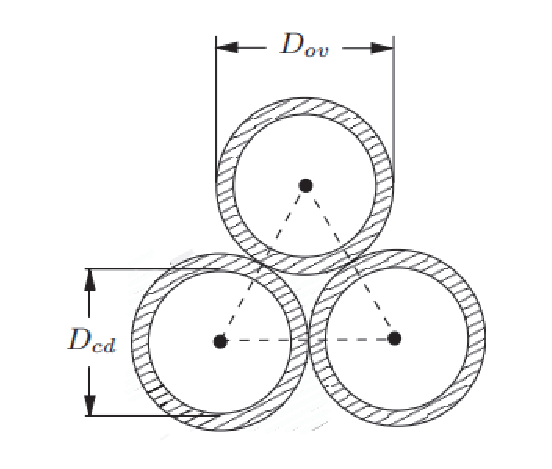
\includegraphics[scale=0.5]{chpt3/figs/fig3.45.eps}
	\caption{紧绕六边形配置下的三根相邻导线。}
\end{figure}


\subsubsection{问题3.16之解}
a)绕组中的平均环箍力为:
\begin{equation}
\tilde{\sigma}=\frac{\sigma_{i}+\sigma_{o}}{2}=\frac{105MPa+65MPa}{2}%(S16.1)
=85MPa\\
\end{equation}

平均绕组半径$\tilde{R}= (a_1 + a_2)/2=87.3 mm$;平均磁场$\tilde{B}_z = (B_i + B_o)/2=4.0 T$。于是,
绕组中的平均环箍力为:
\begin{equation}
\tilde{\sigma}=\tilde{R}(\lambda J)\tilde{B}_{z}=(87.3\times 10^{-3}m)(248\times 10^{6}A/m^{2})(4.0T)%(S16.2)
=86.6 MPa
\end{equation}

这和上文(方程S16.1)计算的$\tilde{\sigma}=(\sigma_i+\sigma_o)/2$几乎一致。

b) 看图3.45中由虚线连城的三角形区域$A_{tr}$,它可由总体导体直径定义:$A_{tr} =\sqrt{3} D_{ov}^2/4$。
三角形内的导体面积$A_{cd}= \pi D_{cd}^2/8$,其中$2.1/3.1$是铜的面积$A_{cu}$,$1/3.1$
是NbTi的面积$A_{sc}$。环氧和绝缘的面积$A_{in}= A_{tr} − A_{cd}$。于是:
\begin{equation}
f_{cu}=\frac{A_{cu}}{A_{ir}}=\frac{\frac{2.1}{3.1}\frac{\pi D_{cd}^{2}}{8}}{\frac{\sqrt{3}}{4}D_{ov}^{2}}=\frac{(2.1)(\pi)(4)(0.63mm)^{2}}{(3.1)(\sqrt{3})(8)(0.71mm)^{2}}=0.484%(S16.3a)
\end{equation}
\begin{equation}
f_{sc}=\frac{A_{sc}}{A_{tr}}=\frac{1}{2.1}\frac{A_{cu}}{A_{tr}}=0.230 %(S16.3b)
\end{equation}
\begin{equation}
f_{in}=\frac{A_{in}}{A_{tr}}=1-\frac{A_{cu}+A_{sc}}{A_{tr}}=1-0.484-0.230=0.286 %(S16.3c)
\end{equation}

c)复合材料的杨氏模量$\tilde{E}$由平行混合法则给出:
\begin{equation}
\tilde{E}=f_{cu}E_{cu}+f_{sc}E_{sc}+f_{in}E_{in}\\%(S16.4)
=(0.48)(100 GPa)+(0.23)(85 GPa)+(0.29)(30 GPa)\\
\simeq 76 GPa
\end{equation}

我们可以计算绕组各组分最内侧半径处的应力:
\begin{eqnarray}
\sigma_{cu}=\sigma_{i}\frac{E_{cu}}{\tilde{E}}=(105MPa)\frac{100GPa}{76GPa}\simeq 137MPa \\%(S16.5a)
\sigma_{sc}=\sigma_{i}\frac{E_{sc}}{\tilde{E}}=(105MPa)\frac{85GPa}{76GPa}\simeq 117MPa \\%(S16.5b)
\sigma_{in}=\sigma_{i}\frac{E_{sc}}{\tilde{E}}=(105MPa)\frac{30GPa}{76GPa}\simeq 41MPa %(S16.5b)
\end{eqnarray}

这些值都忽略了残余应力,而实际上这个力可能很大。
\newpage


\subsection{问题3.17:HTS磁体中的应力和轴向力}
这里我们演示对1.75-T (75 MHz)高温超导内插螺管磁体(由48个双饼线圈堆叠组成)的应力分析[3.58]。
每一个双饼都是由高强度HTS带材绕成的。
HTS内插磁体,运行电流86.7 A,与一个14.1-T (600 MHz)低温超导背景NMR磁体共同组成了675 MHz LTS/HTS
NMR磁体——以后内插磁体将运行电流提高到115.95 A以实现组合磁场16.26 T (692.2 MHz) [3.59]。
表3.9给出了内插磁体和HTS带材(Bi2223/Ag和两层不锈钢层复合材料)的关键参数。 
本例使用的混合法则基于银和不锈钢的机械性能。
表中给出的是双饼线圈的轴向场在中平面外侧的数值$B_z$和$B_r$,这里有最大的应力和应变。

\textbf{应力应变方程}

螺管绕组的径向应力$\sigma_r(r, z)$;环向应力$\sigma_\theta(r, z)$;轴向应力$\sigma_z(r, z)$;
剪切应力$\tau_{rz}$满足的平衡方程已有3.62给出。
\begin{equation}
\frac{\partial\sigma_{r}}{\partial r}+\frac{\sigma_{r}-\sigma_{\theta}}{r}+\frac{\partial\tau_{rz}}{\partial z}=-\lambda JB_{z}(r,z)\\%(3.62a)
\end{equation}
\begin{equation}
\frac{\partial\tau_{rz}}{\partial r}-\frac{\tau_{rz}}{r}+\frac{\partial\sigma_{z}}{\partial z}=-\lambda JB_{r}(r,z)\\%(3.62b)
\end{equation}

边界条件为:$\sigma_r(r = a_1, z) = 0; \sigma_r(a_2, z) = 0; \sigma_z(r, z = \pm b) = 0;
\tau_{rz}(r, \pm b)=0; \tau_{rz}(a_2,\pm b)=0$,
HTS复合材料可以视为正交各向异性的,可以使用Hook定律。当不考虑热应变时,有:
\begin{equation}
\epsilon_{r}=\frac{1}{E_{r}}\sigma_{r}-\frac{v_{rh}}{E_{h}}\sigma_{\theta}-\frac{v_{rz}}{E_{z}}\sigma_{z}\\%(3.171a)
\end{equation}
\begin{equation}
\epsilon_{\theta}=-\frac{v_{hr}}{E_{r}}\sigma_{r}+\frac{1}{E_{h}}\sigma_{\theta}-\frac{v_{hz}}{E_{z}}\sigma_{z}\\%(3.171b)
\end{equation}
\begin{equation}
\epsilon_{z}=-\frac{v_{zr}}{E_{r}}\sigma_{r}-\frac{v_{zh}}{E_{h}}\sigma_{\theta}+\frac{1}{E_{z}}\sigma_{z}\\%(3.171c)
\end{equation}

式中,$\nu_{\xi\eta}$是给定$\epsilon_\xi$和$\sigma_\eta$的Poisson比。

\colorbox{red}{表格3.9}

\colorbox{red}{表格3.10}

表3.10给出了一个饼的忠平面上最内、中点、最外三个点处的应力和环箍应变的数值[3.32]。
中平面轴向力是 −16 kN。
注意到,最大应力出现在绕组最内侧($a_1 =39.10 mm$)。
银的最大组合应力,即Tresca应力 ($\sigma_T= \sigma_{\theta} −\sigma_z$)是56.4 MPa,
这比允许应力($\sigma_{allow}=2\sigma/3(0.2\%)$)要小:银在77K时的允许应力为$\sigma_{allow}\simeq 120 MPa$。

通过解方程3.62和3.171可以得到应力和应变。
但是,3.5部分推导的方程可以用来估计中平面的轴向力。
如上面讨论3.5指出的,HTS磁体在它的中平面上的轴向力计算数值为−16.2 kN (即压缩力),
来自HTS磁体磁场以及HTS和LTS磁体的相互作用。
此处,我们计算HTS磁体的仅由自身磁场贡献的中平面力的近似值。
上面的分析给出的数值是−8.6 kN [3.32]。

a) 将HTS磁体视为“薄壁”的,使用方程3.41a计算$F_z(0)$。选择$a=39.1 mm, b=203.3 mm, NI =5.91\times 10^6 A$。

b) 使用方程3.41b计算$F_z(0)$。分两种情况:1)取HTS磁体的$a_1$,$a=39.1 mm$;2)HTS磁体的绕组平均半,径$a=51.2 mm$。

c) 将HTS磁体视为两个“薄壁”且“长”的子螺管A和B,两者具有相同的绕组厚度。使用方程3.55
计算$F_{zT}(0)$。取$a_A=39.1 mm , a_B=51.2 mm$。

d) 围绕HTS磁体的是一个14.1 T LTS嵌套磁体。将这个LTS磁体建模为薄壁螺管,参数为:$a_B = 191.3 mm;
b_B= 337.5 mm; N_BI_B = 7.535 MA$;HTS内插磁体为薄壁螺管,参数为:$a_A = 51.2 mm; b_A = 203.3 mm;
 N_A I_A = 0.591 MA$。使用方程3.57a,计算HTS内插磁体的总平面轴向力$F_{zA}(0)$。
 这个值是−16.2 kN。解释为什么方程3.57a没有给出正确的值。

e) 两个磁体采用相同的模型,使用方程3.60来计算当HTS内插磁体偏心5mm后其上承受的轴向恢复力。
某程序给出的数值是−2.1 kN。

下面的表3.11-3.14给出了需要的椭圆积分值。

\subsubsection{问题3.17之解}
\colorbox{red}{表3.11}

a)我们得到3.41a:
\begin{equation}
\begin{split}
F_{z}(0)=&-\frac{\mu_{o}}{2}(\frac{NI}{2b})^{2}\{2b\sqrt{4a^{2}+b^{2}}[K(k_{b})-E(k_{b})]\\
&-2b\sqrt{4a^{2}+4b^{2}}[K(k_{2b})-E(k_{2b})]\}%(3.41a)
\end{split}
\end{equation}

式中,$k_b,k_{2b}$是由$a$和$b$决定的模量。本例下,$a=39.1 mm,b=203.3 mm$,我们有:
\begin{eqnarray}
k_b^2=\frac{4a^2}{4a^2+b^2}=0.128888\\
k_{2b}^2=\frac{4a^2}{4a^2+(2b)^2}=0.035670
\end{eqnarray}

所需的完全椭圆积分参数见表3.11。如果应用方程3.38c到$k^6$项,
我们可以在$k^2\ll 1$条件下计算$ K(k)−E(k)$:
\begin{equation}
K(k_{2b})-E(k_{2b})\simeq XXXX=0.106515
\end{equation}

这大致上和表3.11中的计算值$K(k)−E(k)=0.106557$是一致的。

代入$NI =0.591\times 10^6 A$和其他值到方程3.41a,有:
\begin{equation*}
F_z(0)=XXXXXX=-6.2\ \mathrm{kN}
\end{equation*}

这个计算值相比程序值低估了28\%。

\colorbox{red}{表3.12}

b) 方程3.41b得到:
\begin{equation}
\begin{split}
F_{z}(0)&\simeq-\frac{\mu_{o}}{2}(\frac{NI}{2b})^{2}\pi a^{2}\\%(3.41b)
&\simeq-\frac{(4\pi\times 10^{-7}H/m)}{2}[\frac{(5.91\times 10^{5}A)}{0.4066m}]^{2}\pi(0.0391m)^{2}\\
&=-6.4kN
\end{split}
\end{equation}

这是程序值的74\%。用平均半径51.2mm替代 39.1mm得到的力为10.9 kN,比程序值大 27\%。 

c) 如果磁体建模为两个“薄壁”且“长”的螺管,应用方程3.55:
\begin{equation}
F_{zT}(0)\simeq-\mu_{o}(\frac{NI}{4b})^{2}\pi(a_{A}^{2}+a_{B}^{2}){1-\frac{(a_{A}-a_{B})^{2}}{\pi(a_{A}^{2}+a_{B}^{2})}[2\prod(c^{2},k_{b})-\prod(c^{2},k_{2b})]}\\%(3.55)
\end{equation}

对模量$k_b, k_{2b},c^2$,已知$a_T = a_A+a_B, a_A = 39.1 mm, a_B = 51.2 mm, b =203.3 mm, a_T=90.3 mm$。有:
\begin{eqnarray}
c^2=\frac{4a_A a_B)}{a_T^2}=0.982045\\
k_b^2=\frac{4a_A a_B}{a_T^2+b^2}=0.161820\ \Rightarrow k_b=0.402269\\
k_{2b}^2=\frac{4a_A a_B}{a_T^2+4b^2}=0.046160\ \Rightarrow k_{2b}=0.214848
\end{eqnarray}

于是:
$$
F_z(0)=-7.4\ \mathrm{kN}
$$

相比于程序值,低估了15\%。

\colorbox{red}{表3.13}

d)式3.57a下式给出:
\begin{equation}
\begin{split}
F_{zA}(0)\simeq&-\frac{\mu_{o}}{2}\{(\frac{N_{A}I_{A}}{2b_{A}})^{2}\pi a_{A}^{2}+(\frac{N_{B}I_{B}}{2b_{B}})(\frac{N_{A}I_{A}}{2b_{A}})\times\\
&(a_{A}-a_{B})^{2}[\prod(c^{2},k_{D})+\prod(c^{2},k_{T})-2\prod(c^{2},k_{B})]\}%(3.57a)
\end{split}
\end{equation}

不同的参数为:$a_T=a_A+a_B=242.5 mm;b_T=b_A+b_B=540.8 mm; b_D=b_A−b_B=−134.2 mm$;以及:
\begin{eqnarray*}
c^2&=&\frac{4a_A a_B)}{a_T^2}=0.666266\\
k_D^2&=&\frac{4a_A a_B}{a_T^2+b_D^2}=0.510028\ \Rightarrow k_D=0.0.714162\\
k_{T}^2&=&\frac{4a_A a_B}{a_T^2+b_T^2}=0.111533\ \Rightarrow k_{2b}=0.333965\\
k_B^2&=&\frac{4a_A a_B}{a_T^2+b_B^2}=0.226841\ \Rightarrow k_{B}=0.476278
\end{eqnarray*}

将这些值代入方程3.57a,有:
\begin{equation}
F_{zA}(0)\simeq XXXXX =-43.3\ \mathrm{kN}
\end{equation}

这是程序值16.2 kN的2.7倍。主要的错误来自方程3.57a的近似涉及到了相互作用力$F_{zAB}$。
为了让方程3.57a可用,正如在推导时指出的,条件$b_A^2\gg  4a_A^2,b^2_B\gg  a_T^2, b_D^2\gg a_T^2$必须要满足。
在这个特殊的粒子中,我们有$b_A^2/4a_T^2=0.176;b^2_B/a_T^2 = 1.94; b_D^2/a_T^2 = 0.306$,也就是说,
没有一个条件满足。

\colorbox{red}{表3.14}

e)式3.60由下式给出:
\begin{equation}
\begin{split}
F_{zR}(\rho)=&-\frac{\mu_{o}}{2}(\frac{N_{A}I_{A}}{2b_{A}})(\frac{N_{B}I_{B}}{2b_{B}})\times\\
&(\frac{b_{T}-\rho}{\sqrt{a_{T}^{2}+(b_{T}-\rho)^{2}}}\{[a_{T}^{2}+(b_{T}-\rho)^{2}][K(k_{T-})-E(k_{T-})]-\Upsilon(C^{2},K_{T-})\}\\
&+\frac{b_{D}+\rho}{\sqrt{a_{T}^{2}+(b_{D}+\rho)^{2}}}\{[a_{T}^{2}+(b_{D}+\rho)^{2}][K(k_{D+})-E(k_{D+})]-\Upsilon(c^{2},k_{D+})\}\\
&-\frac{b_{T}+\rho}{\sqrt{a_{T}^{2}+(b_{T}+\rho)^{2}}}\{[a_{T}^{2}+(b_{T}+\rho)^{2}][K(k_{T+})-E(k_{T+})]-\Upsilon(c^{2},k_{T+})\}\\
&-\frac{b_{D}+\rho}{\sqrt{a_{T}^{2}+(b_{D}-\rho)^{2}}}\{[a_{T}^{2}+(b_{D}-\rho)^{2}][K(k_{D-})-E(k_{D-})]-\Upsilon(c^{2},k_{D-})\}\\%(3.60)
\end{split}
\end{equation}

不同的参数为:$a_T=a_A+a_B=242.5 mm;b_T=b_A+b_B=540.8 mm; b_D=b_A−b_B=−134.2 mm$;以及
\begin{eqnarray}
c^2=\frac{4a_A a_B)}{a_T^2}=0.666266\\
k_{T+}^2=\frac{4a_A a_B}{a_T^2+(b_T+\rho)^2}=0.109834\ \Rightarrow k_{T+}=0.331412\\
k_{T-}^2=\frac{4a_A a_B}{a_T^2+(b_T-\rho)^2}=0.0.113269\ \Rightarrow k_{T-}=0.336554\\
k_{D+}^2=\frac{4a_A a_B}{a_T^2+(b_D+\rho)^2}=0.0.518925\ \Rightarrow k_{D+}=0.720364\\
k_{D-}^2=\frac{4a_A a_B}{a_T^2+(b_D-\rho)^2}=0.501110\ \Rightarrow k_{D-}=0.707891
\end{eqnarray}

\colorbox{red}{表3.15}

应用表3.15中的数值到方程3.60,我们计算:
$$
a_{2}-a_{1}=[1+\frac{\sqrt{3}}{2}(N_{\ell}-1)]D_{ov}%(3.172)
$$

相比程序值(2.1 N),这个计算值高估了大约4\%;负号表示这个力是恢复力。
磁体间的“弹性常数”大约$400\ \mathrm{kN/m}$。
\newpage


\subsection{讨论3.12:铁球上的磁力}
出于安全考虑,将铁磁物体远离大型磁体放置时很重要的。
举45T混合磁体为例,我们在这里推导“远离”磁体的铁球(图3.46)受到的磁力。
螺管的边缘场(远场)已在问题311论及,可由双极场给出:
\begin{equation}%(3.163)
\vec{H}_{f}=H_{0}(\frac{R_{e}}{r})^{3}(\cos\theta\vec{\imath}_{r}+\frac{1}{2}\sin\theta\vec{\imath}_{\theta})
\end{equation}

当一个磁性物体,比如铁球,处于空间变化的磁场中时,它会受到一个磁场力$\vec{f}_m$:
\begin{equation}
\vec{f}_{m}(r,\theta)=\nabla e_{m}\\%(3.173)
\end{equation}

式中,$\nabla$是球坐标下的梯度算符,$e_m$是铁球因磁化而存储的磁能密度。
对于一个$\mu/\mu_0\gg 1$的铁磁球,球内的磁场$\vec{B}_{sp}$是外加“均匀”磁场的
三倍:$\vec{B}_{sp}\simeq 3\mu_0 \vec{H}_f= 3\vec{B}_f$ (问题2.1)。
对于一个直径远小于其到磁体中心的距离的球,$\vec{B}_f$可以认为在球上各处是一致的:
\begin{equation}
e_{m}=\frac{\vec{B}_{sp}\cdot\vec{B}_{f}}{2\mu_{o}}=\frac{3|\vec{B}_{f}|^{2}}{2\mu_{o}}%(3.174)
\end{equation}

当铁球在磁化$M_{sa}$下饱和时,它的磁场近似为$\vec{B}_{sa} (= \mu_{0}) M_{sa})$,该值是一个常数且与
$\vec{B}_f$同向。磁能密度于是可以写为:
\begin{equation}
e_{ms}\simeq\frac{\vec{B}_{sa}\cdot\vec{B}_{f}}{2\mu_{o}}%(3.17)
\end{equation}

在方程3.174和3.175中,我们假定在计算能量密度时边缘场是均匀的,但是在计算力密度时是不均匀的。
\begin{figure}[htbp]
	\centering
	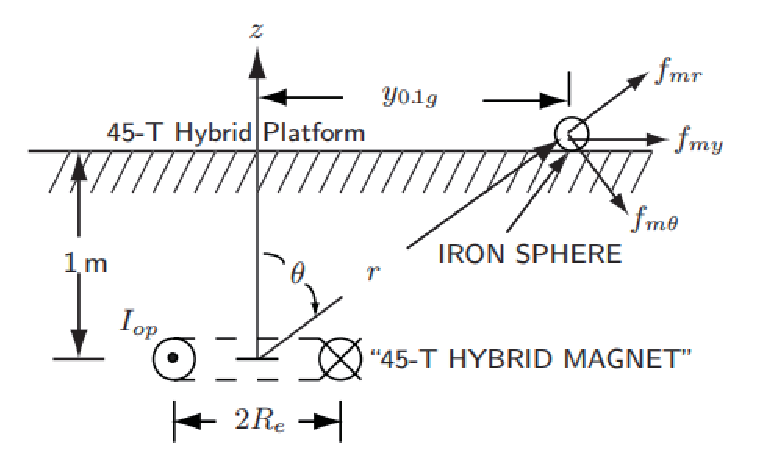
\includegraphics[scale=0.5]{chpt3/figs/fig3.46.eps}
	\caption{处于45T混合磁体平台中的铁球。}
\end{figure}

\textbf{A.不饱和球上的力}

为了推导不饱和铁球上的$\vec{f}_{m}(r,\theta)$表达式,我们首先从方程3.163中计算$|\vec{B}_f|^2$。
\begin{equation}
|\vec{B}_f|^2=\mu_0^2 H_0^2\left(\frac{R_e}{r}\right)^6(\cos^2\theta+\frac{1}{4}\sin^2\theta)
\end{equation}

联立上式和方程3.174,对3.173使用球坐标中的梯度算符,我们得到:
\begin{equation}
\begin{split}
\vec{f}_{m}(r,\theta)=&\frac{3\mu_0 H_0^2}{2}\bigg[(\cos^2\theta+\frac{1}{4}\sin^2\theta\frac{\partial}{\partial r}(\frac{R_e}{r})^6)\vec{\imath}_r\\
&+\frac{1}{r}(\frac{R_e}{r})^6\frac{\partial}{\partial \theta}(\cos^2\theta+\frac{1}{4}\sin^2\theta)\vec{\imath}_\theta\bigg]\\
=&\frac{3\mu_0 H_0^2}{2R_e}(\frac{R_e}{r})^7\left[-6(\cos^2\theta+\frac{1}{4}\sin^2\theta)\vec{\imath}_i-\frac{3}{2}\sin\theta\cos\theta\vec{\imath}_\theta\right]
\end{split}
\end{equation}

我们可以简化为:
\begin{equation}
\vec{f}_{m}(r,\theta)=-\frac{9\mu_{o}H_{0}^{2}}{4R_{e}}(\frac{R_{e}}{r})^{2}[(1+3\cos^{2}\theta)\vec{\imath}_{r}+\sin\theta\cos\theta\vec{\imath}_{\theta}]\\%(3.176a)
\end{equation}

可见,$\vec{f}_{m}(r,\theta)$随$1/r^7$变化。如我们所期的,对于任何铁磁物体,
$\vec{f}_{m}(r,\theta)$的$r$分量指向磁体中心。

\textbf{B.饱和球上的力}

方程3.175给出的磁能密度为:
\begin{equation}
e_{ms}=\mu_0 M_{sa}H_0(\frac{R_e}{r})^3\sqrt{\cos^2\theta+\frac{1}{4}\sin^2\theta}
\end{equation}

类似的,对磁能密度求梯度,我们得到:
\begin{equation}
\begin{split}
\vec{f}_{ms}(r\theta)=&-\frac{3\mu_{o}M_{sa}H_{0}}{2R_{e}}(\frac{R_{e}}{r})^{4}\\
&\times(\sqrt{1+3\cos^{2}\theta\vec{\imath}_{r}}+\frac{\sin\theta\cos\theta}{\sqrt{1+3\cos^{2}\theta}}\vec{\theta})\\%(3.176b)
\end{split}
\end{equation}

可见,当铁球饱和时,磁力随$1/r^4$变化。
因为它和不饱和球中一样,是$-r$向的,铁球被磁体中心所吸引。

\textbf{演示}\quad 就45T混合磁体(仅考虑超导磁体的磁场)而言,其$B_0 = 14 T,R_e = 0.67 m$ (问题3.11),我们可以
计算$y_{0.1g}$。该点位于磁体平台中心($z=2.75 m$)为起点的y轴上,该处施于密度为$\rho$的非饱和铁球磁力密度上的磁力恰为
$f_{my}=0.1\rho g$(0.1倍重力加速度)。$f_{my}$为:
\begin{equation}
f_{my}=f_{mr}\sin\theta+f_{m\theta}\cos\theta%(3.177)
\end{equation}

式中,$f_{mr}$和$f_{m\theta}$分别是磁力的$r$分量和$\theta$分量。联立
方程3.176a和3.177,我们得到:
\begin{equation}
\begin{split}
f_{my}&=\frac{9\mu_{o}H_{0}^{2}}{4R_{e}}(\frac{R_{e}}{r})^{7}[-(1+3\cos^{2}\theta)\sin\theta-\sin\theta\cos^{2}\theta]\\
&=-\frac{9\mu_{o}H_{0}^{2}}{4R_{e}}(\frac{R_{e}}{r})^{7}(1+4\cos^{2}\theta)\sin\theta\\%(3.178)
\end{split}
\end{equation}

方程3.178中的符号表示$f_{my}$实际上指向图3.46中所示的相反方向。在$x=0$时的$r,\sin\theta,\cos\theta$分别为:
\begin{equation*}
r=\sqrt{y_{0.1g}^2+z^2};\qquad \sin\theta=\frac{y_{0.1g}}{\sqrt{y_{0.1g}^2+z^2}};\qquad \cos\theta=\frac{z}{\sqrt{y_{0.1g}^2+z^2}}
\end{equation*}

联立上面的表达式和方程3.178,代入$f_{my}=0.1\rho g$,得到:
\begin{equation*}
0.1\rho g=\frac{9(\mu_0 H_0)^2R_e^6}{4\mu_0}(\frac{1}{y_{0.1g}^2+z^2})^{3.5}(1+\frac{4z^2}{y_{0.1g}^2+z^2})\frac{y_{0.1g}}{y_{0.1g}^2+z^2}
\end{equation*}

代入上面表达式的合适值,并代入$z=2.75 m$,我们得到:
\begin{equation*}
0.1(8000)(9.81)=\frac{9(14)^2(0.67)^6}{4(4\pi\times 10^{-7})}[\frac{1}{y_{0.1g}^2+2.75^2}]^{3.5}\times[1+\frac{4(2.75)}{y_{0.1g}^2+2.75^2}]\frac{y_{0.1g}}{\sqrt{y_{0.1g}^+2.75^2}}
\end{equation*}

解得,$y_{0.1g}\simeq 2.42\ \mathrm{m}$

我们可以算出球上的总场,然后看球是否如计算时假设的那样非饱和。
已知$r_{0.1g} =\sqrt{(2.42 m)^2+(2.75 m)^2}\simeq 3.66 m$以及$\theta = \tan^{−1}(2.42 m/2.75 m) = 41.3^\circ$,
代入方程3.163,有:
\begin{equation*}
\begin{split}
|\mu_0 \vec{H}_f|&=(14.0)(\frac{0.67}{3.66})\sqrt{\cos^2 41.3^\circ+\frac{1}{4}\sin^2 41.3^\circ}\\
&=(14.0)(6.1\times 10^{-3})(0.82)=0.070\ \mathrm{T}\qquad(\vec{M}=3\mu_0\vec{H}_f=0.21\ \mathrm{T})
\end{split}
\end{equation*}
\newpage


\subsection{讨论3.13:两线圈磁体的径向力}
图3.47给出了两线圈磁体的一种布局,其中内线圈1的轴垂直于$z$轴,但相对于外线圈2的轴偏移$\Delta x$。
两个线圈的轴向场都是指向$+z$方向,中平面都位于$z=0$。

当线圈1和线圈2同心,也即$\Delta x=0,\Delta y=0$时,单位绕组体积上的作用力$J_\theta \times B_z$
是$r$向的;根据对称性,可被消除:净轴向力为零。如果线圈1失配$+\Delta x$,如图所示,
那么施加于绕组体积的一半(xy平面上$+x$侧的$180^\circ$弧度)上的$B_{z2}$
平均起来要大于另一半上的$B_{z2}$。最终的净不平衡力$F_{x1}$可以近似表示为:
\begin{equation}%(3.179)
F_{x1}\simeq4\pi\triangle x\int_{0}^{b}\int_{a_{1}}^{a_{2}}J_{\theta1}\frac{\partial B_{z2}(r,z)}{\partial r}r\ dr\ dz\\
\end{equation}

式中,$B_{z2}$是由线圈2产生的轴向力。
如方程3.12b以及3.117a–3.117c(问题3.2)所指出的,$B_{z2}$随着在xy平面上的失配增加而增大,也即
$\partial B_{z2}/\partial r>0$。于是,$F_{x1}$是正的,并且在$x$方向增大;进而线圈1的失配继续扩大:
系统不稳定。

另一种看待这种情况的方法是认识到励磁线圈1总是被吸引到最高场区域。
因此,如果线圈1径向移位,则它继续沿径向朝线圈2移动。原因如上所述:$B_{z2}$随着xy平面中的位移而增加; $B_{z2}$在线圈2的绕组最内圈半径处最大。
相同的理由可用于解释为什么$z$方向上的位移是稳定的:如果线圈1轴向移位$\Delta z$,因为每个线圈的轴向场在中平面($z = 0$)处最大,线圈1试图将其最大场区域与线圈2的区域对齐,从而在$z$方向的失配是稳定的。
\begin{figure}[htbp]
	\centering
	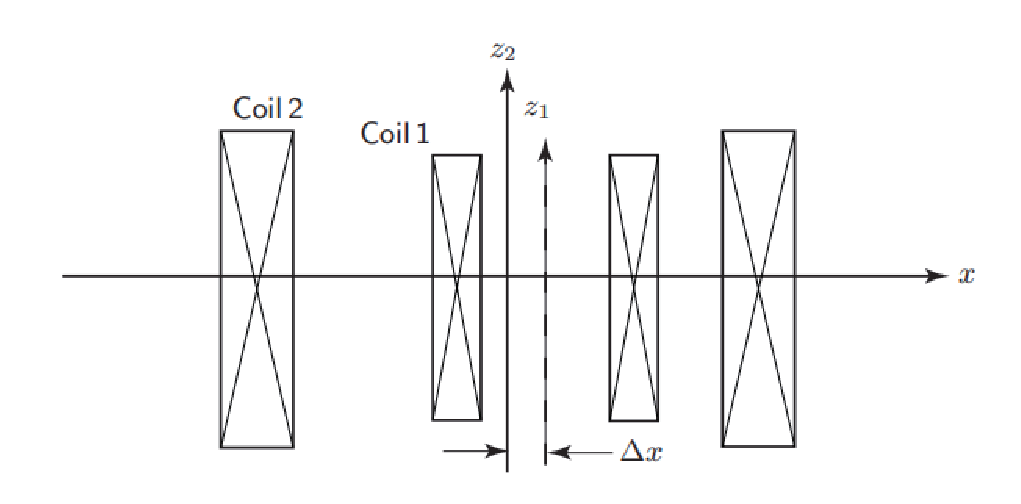
\includegraphics[scale=0.5]{chpt3/figs/fig3.47.eps}
	\caption{Two nested solenoidal coils, one displaced radially from the other}
\end{figure}
\newpage



\subsection{讨论3.14:45 T混合磁体的结构支撑}
45T混合磁体的设计具有后续通过将24MW内插电阻磁体提至35MW从而可在50T运行的潜力。
设计中的一个关键要点是插入磁体和SCM之间传递故障力的结构。
特别关键的是在低温恒温器内部提供热间隙的结构部件。
在45T混合磁体中,该部件是单个圆柱形钢柱,与SCM同轴,with heat intercepts at ∼80K and ∼20 K。
为了计算在插入磁体失效时支撑结构上的潜在故障负荷上限,我们对升级50T进行了下面的分析。
\begin{enumerate}
	\item 分析在以下基础上进行:获取45T电阻内插磁体的尺寸,每个子线圈在峰值时具有均匀电流密度,
	调节每个子线圈中的电流水平调节至50T。该分析给出了一种插入磁体,与具有$1 / r$电流分布的线圈相比,该插入磁体相对于SCM具有固有的更高的磁能和更高的失配力。
	
	\item 基于这种配置,假设最坏情况的故障,即每个子线圈的中平面突然短路,导致电流加倍(恒定电压假设)和每个子线圈的磁中心的轴向移位$b_i$(第i个线圈的半高)。对于假设的子线圈几何结构,这个假设的故障分别导致线圈A,B和C中的力为$\sim 1.7 MN,\sim 1.8 MN$和$\sim 2.5 MN$,即SCM上的力总共约$6 MN$ 。
	精心选择支撑柱的壁厚以确保故障期间的平均应力不超过其$2/3$屈服。按照$1.8-20 K,20-80 K$和$80-300 K$对壁厚进行分级以匹配奥氏体钢屈服应力的温度依赖性。由此产生的传导热输入是系统总低温负荷的一小部分。由此产生的支撑柱设计具有额外的优点,即对轴向和横向载荷都非常坚硬。因此,对于典型的失配力,插入磁体和插入磁体之间的相对偏移非常小。
\end{enumerate}
\newpage



\subsection{讨论3.15:Nb3Sn导体上的应力}
这里我们将讨论$Nb_3Sn$导体的应力问题,主要考虑这种复合导体的青铜、紫铜和$Nb_3Sn$三种材料的应力关系[3.60]。
因为超导体的临界电流密度会因应变而退降——在拉伸时尤甚,所以,超导体的最大应变水平是磁体设计的关键参数。
应变的效果,特别是$NbTi$和$Nb_3Sn$复合超导体,已获得全面的研究[3.61, 3.62];
高温超导体的数据也已成形[3.63, 3.64]。

当$Nb_3Sn$被冷却到$4.2\ \mathrm{K}$,各组分都经历了一个$\sim 1000\ \mathrm{K}$的温度下降:从
$\sim 1000\ \mathrm{K}$的反应温度到$4.2\ \mathrm{K}$的运行温度。
因为各组分的热缩系数不同,各组分中将出现参与残余应力。

图3.48示意了三种应变状态:a)复合物处理反应温度$\sim 1000\ \mathrm{K}$;
b)如果三种组分可以独立收缩时的$4.2\ \mathrm{K}$状态;c)复合物处于$4.2\ \mathrm{K}$。
尽管有所放大,示意图指出了三种组分各自热缩系数从反应温度到运行温度的相对大小,分别记为$\epsilon_{br_0},\epsilon_{cu_0}, \epsilon_{s_0}$。
与此同时,复合物在$4.2\ \mathrm{K}$的残余应变$\epsilon_{br_r},\epsilon_{cu_r}, \epsilon_{s_r}$
也在图中给出。可以看出,青铜和紫铜都将处于拉伸状态,而$Nb_3Sn$处于压缩状态。
图中的$E$和$A$分别代表杨氏模量和截面积,下标指示了组分。
另外,图中的各应变是按照标量处理的。
\begin{figure}[htbp]
	\centering
	\includegraphics[scale=0.5]{chpt3/figs/fig3.48.eps}
	\caption{$Nb_3Sn$复合材料冷却后的应力应变。}
\end{figure}

\textbf{A. 平衡方程}

处于4.2 K的复合材料的应力应变平衡方程为:
\begin{eqnarray}% 3.180a,b,c,d
\epsilon_{br_r}A_{br}E_{br}+\epsilon_{cu_r}A_{cu}E_{cu}-\epsilon_{s_r}A_sE_s&=&0\\
+\epsilon_{br_r}+\epsilon_{s_r}&=&\epsilon_{br_0}-\epsilon_{s_0}\\
-\epsilon_{cu_r}+\epsilon_{s_r}&=&\epsilon_{cu_0}-\epsilon_{s_0}\\
-\epsilon_{cu_r}+\epsilon_{br_r}&=&\epsilon_{cu_0}-\epsilon_{br_0}
\end{eqnarray}

方程3.180a表明净内力为零。
方程3.180b –3.180d给出了青铜/$Nb_3Sn$、紫铜/$Nb_3Sn$、青铜/紫铜各自的应变相容性。
注意方程3.180隐含假定了各组分都处于塑性范围,而事实并不总是这样。

\textbf{B. 残余应变}

从方程3.180b和3.180c,我们可以得到$\epsilon_{s_r}$和$\epsilon_{cu_r}$的表达式:
\begin{eqnarray*}% page206
\epsilon_{s_r}&=\epsilon_{cu_0}-\epsilon_{s_0}-\epsilon_{cu_r}\\
\epsilon_{cu_r}&=\epsilon_{br_r}-\epsilon_{br_0}+\epsilon_{cu_0}
\end{eqnarray*}

将上面的式子与方程3.180联立,有:
\begin{equation*}
\epsilon_{br_r}A_{br}E_{br}+(\epsilon_{br_r}-\epsilon_{br_0}+\epsilon_{cu_0})A_{cu}E_{cu}+(\epsilon_{br_r}-\epsilon_{br_0}+\epsilon_{s_0})A_sE_s=0
\end{equation*}

从上面的方程解出$\epsilon_{br_r}$,有:
 \begin{equation}% 3.181a
\epsilon_{br_r}=\frac{(\epsilon_{br_0}-\epsilon_{cu_0})A_{cu}E_{cu}+(\epsilon_{br_0}-\epsilon_{s_0})A_sE_s}{A_{cu}E_{cu}+A_{br}E_{br}+A_{s}E_{s}}
\end{equation}

类似的,从方程3.180b–3.180d,我们可以得到$\epsilon_{s_r}$和$\epsilon_{br_r}$:
\begin{eqnarray*}
\epsilon_{s_r}&=\epsilon_{cu_0}-\epsilon_{s_0}-\epsilon_{cu_r}\\
\epsilon_{br_r}&=\epsilon_{br_0}-\epsilon_{cu_0}+\epsilon_{cu_r}
\end{eqnarray*}

于是:
\begin{equation*}
(\epsilon_{br_0}-\epsilon_{cu_0}+\epsilon_{cu_r})A_{br}E_{br}+\epsilon_{cu_r}A_{cu}E_{cu}+(\epsilon_{cu_r}-\epsilon_{cu_0}+\epsilon_{s_0})A_sE_s=0
\end{equation*}

从上面的方程中解出$\epsilon_{cu_r}$:
\begin{equation}% 3.181b
\epsilon_{cu_r}=\frac{(\epsilon_{cu_0}-\epsilon_{br_0})A_{br}E_{br}+(\epsilon_{cu_0}-\epsilon_{s_0})A_sE_s}{A_{cu}E_{cu}+A_{br}E_{br}+A_{s}E_{s}}
\end{equation}

同时,
\begin{eqnarray*}
\epsilon_{br_r}&=\epsilon_{br_0}-\epsilon_{s_0}-\epsilon_{s_r}\\
\epsilon_{cu_r}&=\epsilon_{cu_0}-\epsilon_{s_0}-\epsilon_{s_r}
\end{eqnarray*}

于是
\begin{equation*}
(\epsilon_{br_0}-\epsilon_{s_0}-\epsilon_{s_r})A_{br}E_{br}+(\epsilon_{cu_0}-\epsilon_{s_0}-\epsilon_{s_r})A_{cu}E_{cu}-\epsilon_{s_r}A_sE_s=0
\end{equation*}

从上面的方程解出$\epsilon_{sr}$,有:
\begin{equation}% 3.181c
\epsilon_{s_r}=\frac{(\epsilon_{cu_0}-\epsilon_{s_0})A_{cu}E_{cu}+(\epsilon_{br_0}-\epsilon_{s_0})A_{br}E_{br}}{A_{cu}E_{cu}+A_{br}E_{br}+A_{s}E_{s}}
\end{equation}

\textbf{数值解}\ 使用方程3.181a — 3.181c,以及表3.16给出的各组分数值,我们可以计算
$\epsilon_{br_r},\epsilon_{cu_r}, \epsilon_{s_r}$:
\begin{eqnarray*}% page207
\begin{split}
\epsilon_{br_r}&=\frac{(1.66-1.62)(0.62)(100\ \mathrm{GPa})+(1.66-0.72)(0.14)(165\ \mathrm{GPa})}{(0.24)(100\ \mathrm{GPa})+(0.62)(100\ \mathrm{GPa})+(0.14)(165\ \mathrm{GPa})}\\
&=(\frac{22.19\ \mathrm{GPa}}{109.1\ \mathrm{GPa}})\% \simeq0.22\% \\
\epsilon_{cu_r}&=\frac{(1.62-1.66)(0.24)(100\ \mathrm{GPa})+(1.62-0.72)(0.14)(165\ \mathrm{GPa})}{62.9\ \mathrm{GPa}}\\
&=(\frac{19.83\ \mathrm{GPa}}{109.1\ \mathrm{GPa}}\%)\simeq0.18\% \\
\epsilon_{s_r}&=\frac{(1.62-0.72)(0.62)(100\ \mathrm{GPa})+(1.66-0.72)(0.24)(100\ \mathrm{GPa})}{62.9\ \mathrm{GPa}}\\
&=(\frac{78.36\ \mathrm{GPa}}{109.1\ \mathrm{GPa}}\%)\simeq0.72\% 
\end{split}
\end{eqnarray*}

注意到两种基底材料都处于拉伸状态,而$Nb_3Sn$处于压缩状态;
0.72\%的$\epsilon_{s_r}$还是太大了,几乎可以肯定会破坏导体。
不过,当磁体励磁后,导体基本处于拉伸张力状态,这会令$\epsilon_{s_r}$有零应变的倾向;
通常,磁体励磁后,Lorentz应力足以让$Nb_3Sn$处于拉伸应变状态了。

\textbf{C.青铜和紫铜中的应力}

从上文计算的$\epsilon_{br_r},\epsilon_{cu_r}$,我们可以计算响应的应力:
 \begin{eqnarray*}
\sigma_{br_r}&=\epsilon_{br_r}E_{br}\simeq(2.2\times10^{-3})(100\times10^9Pa)\simeq220\ \mathrm{MPa}\\
\sigma_{cr_r}&=\epsilon_{cr_r}E_{cr}\simeq(1.8\times10^{-3})(100\times10^9Pa)\simeq180\ \mathrm{MPa}
\end{eqnarray*}

退火青铜的屈服应力$\sigma_{br_y}$,退火紫铜的屈服应力$\sigma_{cu_y}$仅
$\sim 100\ \mathrm{MPa}$;青铜和紫铜在冷却过程中都是塑性屈服的。

%%表3.16
\colorbox{red}{表格3.16}

\newpage



\subsection{问题3.18:部分系统的自感}
推导3.7.3节给出的“低频”自感公式。

a) 半径为$a$的导线内部的单位长度电感为:
 \begin{equation}% 3.83
L=\frac{\mu_0}{8\pi}
\end{equation}

b) N匝“特别长”($\beta\gg \alpha$)的薄线圈的自感:
 \begin{equation}% 3.84c
L=\mu a_1N62\left(\frac{\pi}{2\beta}\right)
\end{equation}

c) “理想”N匝双极线圈单位长度自感:
 \begin{equation}% 3.87
L=\frac{1}{8}\mu_0\pi N^2
\end{equation}

使用两种表达式:1) $L= 2E_m/I^2$;和2)$ L=N\Phi$推导上式(方程3.87)。
\begin{equation}% 3.88
L=\frac{1}{16}\mu_0\pi N^2
\end{equation}

e) 主半径为$R$,圆形截面半径$a$,共N匝的“理想”环形线圈的自感:
 \begin{equation}%3.89a
L=\mu_0 R N^2\left[1-\sqrt{1-\left(\frac{a}{R}\right)}\right]
\end{equation}

f) 在极限$a\ll R$下,e)中理想环线圈的自感:
 \begin{equation}% 3.89b
L=\mu_0aN^2(\frac{a}{2R})[1+\frac{1}{4}(\frac{a}{R})^2+\frac{1}{8}(\frac{a}{R})^4\cdots]
\end{equation}

g) 主半径为$R$,矩形截面宽$2a$(r轴)、高$2b$(z轴),共N匝的“理想”环形线圈的自感:
 \begin{equation}% 3.90a
L=\mu_0 b N^2\left[\frac{1}{\pi}\ln\left(\frac{R+a}{R-a}\right)\right]
\end{equation}

h) 在极限$a\ll R$下,g)中理想环线圈的自感:
 \begin{equation}% 3.90b
L=\mu_0bN^2(\frac{2a}{\pi R})[1+\frac{1}{3}(\frac{a}{R})^2+\frac{1}{5}(\frac{a}{R})^4\cdots]
\end{equation}

\subsubsection{问题3.18之解}
a) 一条半径为$a$的导线,通过均匀分布于其截面的电流$I$,内部的磁场为:
 \begin{equation}% S18.1
H_\theta(r)=\frac{I}{2\pi a^2}r
\end{equation}

导体内部单位长度储存的磁场能$e_m$为:
 \begin{equation}%S18.2
e_m=\frac{1}{2}\mu_0\int_{0}^{a}2\pi H_{\theta}^{2}(r)rdr
\end{equation}

联立方程S18.1和S18.2,我们有:
 \begin{equation}%S 18.3
e_m=\frac{\mu_0}{16\pi}I^2
\end{equation}

联立方程3.79 ($E_m =LI^2/2$;单位长度$e_m =LI^2/2$)和S18.3,
解出导线内部的自感$L$:
 \begin{equation}% 3.83
L=\frac{\mu_0}{8\pi}
\end{equation}

b) 根据方程3.111d,长螺管($\beta\gg\alpha$)的中心场$B_z(0, 0)$为$\mu_0 NI/2b$。
从方程3.117c可以得出,“薄壁”和“长”螺管的磁场在轴向和径向都是均匀分布的,并且等于中心场。
于是,螺管的N匝交链的总磁链为:
 \begin{equation}% S18.4
\Phi=\int_{0}^{a_1}2\pi rH_z(0,0)dr=N\left(\frac{\pi a_{1}^{2}\mu_0NI}{2b}\right)
\end{equation}

联立方程3.78 ($\Phi=LI$)和S18.4,我们得到:
 \begin{equation}% 3.84c
L=\mu_0a_1N^2(\frac{\pi}{2\beta})
\end{equation}

c)\textbf{方法一:能量} \ 如问题3.8所给出的,理想双极线圈的总安匝($NI$):
\begin{equation}% S18.5
NI=\int_{-\frac{\pi}{2}}^{\frac{\pi}{2}}K_f Rd\theta
\end{equation}

式中,$R$是双极半径。联立3.140 ($\vec{K}_f$)和S18.5,有:
\begin{equation}% S18.6
NI=\int_{-\frac{\pi}{2}}^{\frac{\pi}{2}}2H_0R\cos\theta d\theta=4H_0R
\end{equation}

双极磁体的单位长度总磁能$E_m$由方程3.143表示:
 \begin{equation}% 3.143
E_m=\frac{\pi R^2B_{0}^{2}}{\mu_0}
\end{equation}

下面我们从方程S18.6计算$H_0R=NI/4$。联立3.143和3.79,解出$L_\ell$ (单位长度的$L$),有:
 \begin{equation}% 3.87
L_\ell=\frac{1}{8}\mu_0\pi N^2
\end{equation}

\textbf{方法二:磁链}\ 首先,表面电流密度$\vec{K}_f$在双极绕组上不均匀。方程3.140指出,$\vec{K}_f=-2H_0\cos\theta\vec{i_z}$。
如果$I$在绕组中均匀分布,则“匝密度”$n(\theta)$必须如下随$\theta$变化:
\begin{equation}% S18.7
n_(\theta)=\frac{1}{2}N\cos\theta
\end{equation}

因为双极磁体有一个均匀分布的磁场$H_0$,双极的N匝总交链为:
\begin{equation}% S18.8
\begin{split}
N\Phi&=\int_{-\frac{\pi}{2}}^{\frac{\pi}{2}}n(\theta)\mu_0H_0(2R\cos\theta)d\theta=
\mu_0NH_0R\int_{-\frac{\pi}{2}}^{\frac{\pi}{2}}\cos\theta^2d\theta \\
&=\frac{1}{2}\mu_0\pi H_0 R=\frac{1}{8}\mu_0\pi N^2I
\end{split}
\end{equation}

联立方程S18.8和3.78,我们有:
 \begin{equation}% 3.87
L_\ell=\frac{1}{8}\mu_0\pi N^2
\end{equation}

d) \textbf{方法一:能量}\ 理想四极磁体(问题3.9)的总安匝$NI$为:
\begin{equation}% S18.9
NI=2\times\int_{-\frac{\pi}{4}}^{\frac{\pi}{4}}K_fRd\theta
\end{equation}

$R$是四极磁体的半径。积分前面的乘数2的原因可由图3.35(b)看出,即电流分布被分到两个区域,我们只考虑了一极。
联立方程3.146和 ($\vec{K}_f$)和S18.9,我们有:
 \begin{equation}% S18.10
NI=2\times\int_{-\frac{\pi}{4}}^{\frac{\pi}{4}}2H_0R\cos 2\theta d\theta=4H_0R
\end{equation}

四极磁体单位长度的总磁能在整个表面积分$\mu_0|H(r,\theta)|^2/2$获得。
方程3.145给出的$|H(r,\theta)|^2$与$\theta$无关,因为$\sin^2 2\theta+\cos^2 2\theta=1$:
\begin{equation}% S18.11
\begin{split}
E_m&=\frac{1}{2}\mu_0(\frac{H_0}{R})^2\int_{0}^{R}2\pi r^3dr+\frac{1}{2}\mu_0H_{0}^{2}R^6\int_{R}^{\infty}\frac{2\pi dr}{r^5}\\
&=\frac{1}{2}\mu_0\pi H_{0}^{2}R^2
\end{split}
\end{equation}

联立3.79、S18.10和S18.11,我们得到:
 \begin{equation}% 3.88
L_\ell=\frac{1}{16}\mu_0\pi N^2
\end{equation}

理想四极磁体的$E_m$是理想双极磁体的$1/2$很容易理解:四极磁场在室温孔内是从$0$到$H_0$变化的,而不是像双极磁场是均匀的;
同时,四极磁体在外部按$1/r^3$衰减,而不是像双极磁体按$1/r^2$衰减。

\textbf{方法二:磁链}\ 类似于上面处理的双极磁体的“匝密度”,四极磁体的匝密度也必须随$\theta$按下式变化:
 \begin{equation}% S18.12
n(\theta)=\frac{1}{2}N\cos 2\theta
\end{equation}

注意到,对上式在$1/4$区域内积分,比如从$-45^\circ$到$45^\circ$,它将给出也必须给出该部分的总匝数$N/2$。
对理想四极磁体,总磁链$\Phi$由下式给出:
\begin{equation}% S18.13b
n\Phi=2\times\int_{-\frac{\pi}{4}}^{\frac{\pi}{4}}n(\theta)\phi(R,\theta)d\theta
\end{equation}

因为$H_{1r} = H_0(r/R) \sin 2\theta$ (方程3.145a),我们有:
 \begin{equation}% 18.13b
\phi(R,\theta)d\theta=2\mu_0H_0R\int_{0}^{\theta}\sin 2\omega d\omega=\mu_0H_0R\cos 2\theta
\end{equation}

于是:
 \begin{equation}% S18.4
N\Phi=\mu_0NH_0R\int_{-\frac{\pi}{4}}^{\frac{\pi}{4}}(\cos)^22\theta d\theta
=\frac{1}{4}\mu_0\pi NH_0R=\frac{1}{16}\mu_0\pi N^2I
\end{equation}

联立3.78和S18.14,我们有:
 \begin{equation}% 3.88
L_\ell=\frac{1}{16}\mu_0\pi N^2
\end{equation}

e) 正如在问题3.10中讨论的,理想圆截面环线圈内部的场$H(r)$是绕向角$(\phi)$向的。根据方程3.161:
 \begin{equation}% S18.15
H_\varphi(r)=\frac{NI}{2\pi r}
\end{equation}

环形线圈的总磁链$\Phi$于是为:
\begin{equation}% S18.16
\Phi=\mu_0N\int_{R-a}^{R+a}\int_{z=-a}^{z=+a}H(r)dzdr
\end{equation}

定义圆截面的方程为:
 \begin{equation}% 18.17
z^2+(R-r)^2=a^2
\end{equation}

在方程S18.16的积分中,对$r$和常数从S18.17中解出$z$并与方程S18.15联立后,有:
\begin{equation}% S18.18
\begin{split}
\Phi&=\frac{\mu_0N^2}{2\pi}\int_{R-a}^{R+a}\int_{-\sqrt{a^2-(R-r)^2}}^{\sqrt{a^2-(R-r)^2}}\frac{dzdr}{r}\\
&=\frac{\mu_0N^2I}{\pi}\int_{R-a}^{R+a}\frac{\sqrt{a^2-R^2+2Rr-r^2}}{r}dr
\end{split}
\end{equation}

\begin{equation}% S18.19
\begin{split}
\Phi&=\frac{\mu_0N^2I}{\pi}\mid R(\sin)^{-1}(\frac{2r-2R}{2a})+\frac{(a^2-R^2)}{\sqrt{R^2-a^2}}(\sin)^{-1}(\frac{2Rr+2a^2-2R^2}{2ra})\mid_{R-a}^{R+a} \\
&=\frac{\mu_0N^2I}{\pi}(R\pi+\pi\frac{a^2-R^2}{\sqrt{R^2-a^2}})=\mu_0N^2RI[1-\sqrt{1-(\frac{a}{R})^2}]
\end{split}
\end{equation}

联立3.78和S18.19,我们得到:
 \begin{equation}% 3.89a
L=\mu_0RN^2\left[1-\sqrt{1-\left(\frac{a}{R}\right)^2}\right]
\end{equation}

f) 对$a\ll R$,我们有:
\begin{equation}% S18.20
\sqrt{1-\left(\frac{a}{R}\right)^2}=1-\frac{1}{2}(\frac{a}{R})^2-\frac{1}{8}(\frac{a}{R})^4-\frac{1}{16}(\frac{a}{R})^6\cdots
\end{equation}

从3.89a和S18.20,
\begin{equation}
L=\mu_0RN^2\left[\frac{1}{2}(\frac{a}{R})^2+\frac{1}{8}(\frac{a}{R})^4+\frac{1}{16}(\frac{a}{R})^6\cdots\right]
\end{equation}

于是
 \begin{equation}% 3.89b
L=\frac{\mu_0a^2N^2}{2R}\left[1+\frac{1}{4}(\frac{a}{R})^2+\frac{1}{8}(\frac{a}{R})^4\cdots\right]
\end{equation}

g) 本理想矩形截面环线圈内部的磁场与上面研究过的圆截面环线圈是一样的,即:
 \begin{equation}% S18.21
N\Phi=\frac{\mu_0N^2I}{2\pi}\int_{R-a}^{R+a}\int_{z=-b}^{z=+b}\frac{1}{r}dzdr
=\frac{\mu_0N^2bI}{\pi}\ln\left(\frac{R+a}{R-a}\right)
\end{equation}

联立3.78和S18.21,我们有:
 \begin{equation}% 3.90a
L=\frac{\mu_0bN^2}{\pi}\ln\left(\frac{R+a}{R-a}\right)
\end{equation}

h) 对$a\ll R$,我们可以展开$\ln(1\pm a/R)$:
 \begin{equation}% S18.22
\ln(1\pm\frac{a}{R})=\pm\frac{a}{R}-\frac{1}{2}(\frac{a}{R})^2\pm\frac{1}{3}(\frac{a}{R})^3-\frac{1}{4}(\frac{a}{R})^4\pm\frac{1}{5}(\frac{a}{R})^5\cdots
\end{equation}

联立3.90a和S18.22,我们得到:
 \begin{eqnarray}% 3.90b
L&=\frac{\mu_0bN^2}{\pi}\left[2(\frac{a}{R})+\frac{2}{3}(\frac{a}{R})^3+\frac{2}{5}(\frac{a}{R})^5\cdots\right]\\
L&=\frac{2\mu_0abN^2}{\pi R}\left[1+\frac{1}{3}(\frac{a}{R})^2+\frac{1}{5}(\frac{a}{R})^4\cdots\right]
\end{eqnarray}

\newpage



\subsection{讨论3.16:Rogowski线圈的互感}
问题2.11中研究过的Rogowski线圈的总磁链表达式为:
 \begin{equation}% 2.69
\Phi(t)\simeq\frac{\mu_0Nc^2}{2R}I(t)
\end{equation}

式中,$R$是Rogowski线圈半径,$c$是每一匝的半径。
方程2.69在$(c/R)^4\ll 1$时有效的,大多数Rogowski线圈通常都能满足这个条件。
电流源和Rogowski线圈之间的互感$M_{ri}$于是可由下式给出:
\begin{equation}% 3.182
M_{ri}\equiv\frac{\Phi}{I}\simeq\frac{\mu_0Nc^2}{2R}
\end{equation}

\newpage



\subsection{讨论3.17:力 vs. 互感}
根据讨论3.12中的方程3.173,$\vec{f_m}(r,\theta)=\nabla e_m$,我们可以由两个“环”线圈
的互感$M_{AB}$导出其轴向力的表达式,反之亦然。
这里,我们研究一个简单情况:两个“环”线圈距离“很远”,$F_{zA}(\rho)$由方程3.39c给出,
$M_{AB}$由方程3.97给出。即:
 \begin{equation}% 3.39c
F_{zA}(\rho)=\frac{3\mu_0}{2\pi}\left(\frac{\pi a_{A}^{2}N_AI_A}{\rho^2}\right)\left(\frac{\pi a_{B}^{2}N_BI_B}{\rho^2}\right)
\end{equation}

以及
\begin{equation}% 3.97
M_{AB}\simeq\frac{\mu_0}{2\pi}\left[\frac{(\pi a_{A}^{2}N_A)(\pi a_{B}^{2}N_B)}{\rho^3}\right]
\end{equation}

对这个系统,我们有:
\begin{equation}% 3.183
e_m=I_AI_BM_{AB}
\end{equation}

在$\rho$方向应用方程3.173,并与方程3.97和3.182联立,得:
\begin{eqnarray}% 3.184a 3.184b 3.184c
F_{zB}(\rho)&=&I_A I_B\frac{dM_{AB}}{d\rho}\\
&=&I_A I_B\frac{d}{d\rho}\left\{\frac{\mu_0}{2\pi}\left[\frac{(\pi a_{A}^{2}N_A)(\pi a_{B}^{2}N_B)}{\rho^3}\right]\right\}\\
&=&-\frac{3\mu_0}{2\pi}\left(\frac{\pi a_{A}^{2}N_A I_A}{\rho^2}\right)\left(\frac{\pi a_{A}^{2}N_B I_B}{\rho^2}\right)
\end{eqnarray}

注意方程3.184a中的$d/d\rho$运算。它是线圈B运动了距离$\partial\rho$,于是
$F_{zB}(\rho)$指向$\rho$相反的方向。也即:
\begin{equation}% 3.39c
F_{zA}(\rho)=-F_{zB}(\rho)
=\frac{3\mu_0}{2\pi}\left(\frac{\pi a_{A}^{2}N_A I_A}{\rho^2}\right)\left(\frac{\pi a_{A}^{2}N_B I_B}{\rho^2}\right)
\end{equation}

很明显,上面的过程反过来就可以用于在已知$F_{zA}(\rho)$时求$M_{AB}$。再次提醒注意:一定要注意符号。
\begin{eqnarray}% 3.185
M_{AB}&=&-\frac{1}{I_AI_B}\int_{0}^{\rho}F_{zA}(y)dy\\
&=&\frac{\mu_0}{2\pi}\left[\frac{(\pi a_{A}^{2}N_A)(\pi a_{B}^{2}N_B)}{\rho^3}\right]
\end{eqnarray}